\documentclass[oneside]{book}

\usepackage{amsmath,amsthm,amssymb,bm}
\usepackage{hyperref}
\usepackage{a4wide}
\usepackage{cleveref}
% \usepackage{refcheck}
\usepackage{graphicx,color}
\usepackage{tikz}
\usepackage{ytableau}
\numberwithin{equation}{section}
\usetikzlibrary{snakes}

\usepackage{enumerate}
\renewcommand\labelenumi{(\theenumi)}
\setcounter{MaxMatrixCols}{20}


\newtheorem{thm}{Theorem}[section]
\newtheorem{lem}[thm]{Lemma}
\newtheorem{prop}[thm]{Proposition}
\newtheorem{cor}[thm]{Corollary}
\theoremstyle{definition}
\newtheorem{exam}[thm]{Example}
\newtheorem{defn}[thm]{Definition}
\newtheorem{conj}[thm]{Conjecture}
\newtheorem{question}[thm]{Question}
\newtheorem{problem}[thm]{Problem}
\newtheorem{remark}[thm]{Remark}
\newtheorem*{note}{Note}

% DO NOT DELETE THIS COMMENT!!! MACROS BELOW:
\newcommand\PD{\operatorname{PD}}
\newcommand\dc{\operatorname{dc}}
\newcommand\NC{\operatorname{NC}}
\newcommand\PM{\operatorname{PM}}
\newcommand\IPM{\operatorname{IPM}}
\newcommand\fix{\operatorname{fix}}
\newcommand\st{\operatorname{st}}
\newcommand\NI{\operatorname{NI}}
\newcommand\LRmax{\operatorname{LRmax}}
\newcommand\zero{\operatorname{zero}}
\newcommand\LRmin{\operatorname{LRmin}}
\newcommand\LH{\operatorname{LH}}
\newcommand\block{\operatorname{block}}
\newcommand\CH{\operatorname{CH}}
\newcommand\CM{\operatorname{CM}}
\newcommand\HH{\operatorname{HH}}
\newcommand\evencycle{\operatorname{evencycle}}
\newcommand\inv{\operatorname{inv}}
\newcommand\cycle{\operatorname{cycle}}
\newcommand\Motz{\operatorname{Motz}}
\newcommand\Fix{\operatorname{Fix}}
\newcommand\sgn{\operatorname{sgn}}
\newcommand\sym{\mathfrak{S}}
\newcommand\invol{\mathfrak{I}}
\newcommand\NN{\mathbb{N}}
\newcommand\QQ{\mathbb{Q}}
\newcommand{\CC}{\mathbb{C}}
\newcommand{\ZZ}{\mathbb{Z}}
\newcommand{\RR}{\mathbb{R}}
\newcommand\LL{\mathcal{L}}
\newcommand\FF{\mathbb{F}}
\newcommand\FT{\operatorname{FT}}

\newcommand{\Dyck}{\operatorname{Dyck}}

\newcommand\Par{\operatorname{Par}}
\newcommand\RPP{\operatorname{RPP}}
\newcommand\SSYT{\operatorname{SSYT}}
\newcommand\SYT{\operatorname{SYT}}

\newcommand\wt{\operatorname{wt}}

\renewcommand\vec[1]{\bm{#1}}
\newcommand\vx{\vec{x}}
\newcommand\vb{\vec{b}}
\newcommand\vla{\vec{\lambda}}
\newcommand\flr[1]{\left\lfloor #1\right\rfloor}
\newcommand\norm[1]{\lVert #1\rVert}
\newcommand\Qbinom[3]{\genfrac{[}{]}{0pt}{}{#1}{#2}_{#3}}
\newcommand\qbinom[2]{\Qbinom{#1}{#2}{q}}

\newcommand\hyper[5]{{}_{#1}F_{#2} \left(#3;#4;#5\right)}
\newcommand\qhyper[5]{{}_{#1}\phi_{#2} \left(#3;#4;#5\right)}
\newcommand\Hyper[5]{{}_{#1}F_{#2} \left( \left.
    \begin{matrix}
      #3\\
      #4\\
    \end{matrix}
    \:\right|\: #5
    \right)}
\newcommand\qHyper[5]{{}_{#1}\phi_{#2} \left(
    \begin{matrix}
      #3\\
      #4\\
    \end{matrix}
    ; #5
    \right)}

\newcommand\comment[1]{\textcolor{gray}{\bf #1}}
\renewcommand\emph[1]{\textcolor{blue}{\bf #1}}


\def\addable(#1,#2){\draw [cyan, line width=1pt] (#1,#2) circle [radius=6pt];}
\def\remove(#1,#2){\fill [cyan] (#1,#2) circle [radius=4pt];}
\def\BM#1{\draw [line width=2pt] (#1+0.9,0.9) rectangle +(-0.8,-0.8);} 
\def\RM#1{\draw [line width=2pt,red] (#1+0.9,0.9) rectangle +(-0.8,-0.8);}
\def\BD#1{\draw [line width=2pt] (#1+0.9,0.9) rectangle +(-1.8,-0.8);}
\def\RD#1{\draw [line width=2pt,red] (#1+0.9,0.9) rectangle +(-1.8,-0.8);}
\def\LRM#1{\RM{#1} \node at (#1+0.5, 1.3) {$x$};}
\def\LBM#1{\BM{#1} \node at (#1+0.5, 1.3) {$-b_{#1}$};}
\def\LBD#1{\BD{#1} \node at (#1, 1.3) {$-\lambda_{#1}$};}
% \def\LRD#1{\RD{#1} \node at (#1, 1.3) {$-\lambda_{#1}$};}

\def\fcirc{\,\tikz\draw[fill] (0,0) circle (2pt);\,}

\newcommand\ulabel[3]{\node at (#1+0.3,#2+0.7) {\( #3 \)};}
\newcommand\hlabel[3]{\node at (#1+0.5,#2+0.3) {\( #3 \)};}
\newcommand\dlabel[3]{\node at (#1+0.7,#2-0.3) {\( #3 \)};}

%%%%%%%%%%%%%%%%%%%%%%%%%%%%%%%%%%%%%%%%%%%%%%%%%%%%%%%%%%%%%%%%

\title{Lecture notes on combinatorics of orthogonal polynomials}
\author{Jang Soo Kim}
% \thanks{The author was supported by NRF grants \#2022R1A2C101100911 and \#2016R1A5A1008055.} 
% \address{Department of Mathematics,
% Sungkyunkwan University (SKKU), Suwon, Gyeonggi-do 16419, South Korea}
% \email{jangsookim@skku.edu}
\date{\today}

\begin{document}

% \begin{abstract}
% \end{abstract}


\maketitle
\tableofcontents

%%%%%%%%%%%%%%%%%%%%%%%%%%%%%%%%%%%%%%%%%%%%%%%%%%%%%%%%%%%%%%%%
% start here

\chapter{Introduction}

Orthogonal polynomials are classical objects arising from the study of
continued fractions. Due to the long history of orthogonal
polynomials, they have now become important objects of study in many
areas: classical analysis and PDE, mathematical physics, probability,
random matrix theory, and combinatorics.

The combinatorial study of orthogonal polynomials was pioneered by
Flajolet and Viennot in 1980s. In these lecture notes we will learn
fascinating combinatorial properties of orthogonal polynomials.

We will first study basic properties of orthogonal polynomials based
on Chihara's book, Chapter~1 \cite{Chihara}. We will then focus on the
combinatorial approach of orthogonal polynomials, which will be based
on Viennot's lecture notes \cite{ViennotLN}. We will also cover more
recent developments in the combinatorics of orthogonal polynomials
such as their connections with ASEP, staircase tableaux, lecture hall
partitions, and orthogonal polynomials of type \( R_1 \).

In \Cref{sec:basics-orth-polyn} we study elementary and classical
results of orthogonal polynomials. In \Cref{cha:basics-enum-comb} we
review basics of enumerative combinatorics. Starting from
\Cref{sec:comb-interpr-orth} we focus on the combinatorics of
orthogonal polynomials.

\chapter{Basics of orthogonal polynomials}
\label{sec:basics-orth-polyn}

In this chapter we will cover the first chapter of Chihara's book
\cite{Chihara}.

\section{Introduction}

Since
\[
  2\cos m\theta \cos n\theta  = \cos(m+n)\theta + \cos(m-n)\theta,
\]
for nonnegative integers \( m \) and \( n \), we have
\begin{equation}\label{eq:coscos=0}
  \int_0^\pi \cos m\theta \cos n\theta d\theta = 0, \qquad m\ne n.
\end{equation}
In this situation we say that \( \cos m\theta \) and
\( \cos n\theta \) are orthogonal over the interval \( (0,\pi) \).

Note that \( \cos n\theta \) is a polynomial in \( \cos\theta \) of
degree \( n \). So we can write \( \cos n\theta = T_n(\cos\theta) \)
for a polynomial \( T_n(x) \) of degree \( x \).

By the change of variable \( x=\cos \theta \), \eqref{eq:coscos=0} can
be rewritten as
\[
  \int_{-1}^1 T_m(x)T_n(x) (1-x^2)^{-1/2} dx = 0, \qquad m\ne n.
\]

The polynomials \( T_n(x) \), \( n\ge0 \), are called the
\emph{Tchebyshev polynomials of the first kind}.
The first few polynomials are:
\begin{align*}
 T_0(x) &= 1, \\
 T_1(x) &= \cos\theta = x, \\
 T_2(x) &= \cos2\theta = 2\cos^2\theta-1 = 2x^2-1, \\
 T_3(x) &= 4x^3-3x.
\end{align*}

Recall that in an inner product space \( V \) with inner product
\( \langle \cdot,\cdot \rangle \), a set of vectors
\( v_1,\dots,v_n \) are said to be orthogonal if
\( \langle v_i,v_j \rangle = 0 \) for all \( i\ne j \). In this sense
the Tchebyshev polynomials \( T_n(x) \) are orthogonal, where
\( V = \RR[x] \) is the space of polynomials with real coefficients
with the inner product given by
\[
  \langle f(x), g(x) \rangle = \int_{-1}^1 f(x)g(x) (1-x^2)^{-1/2} dx.
\]
We say that \( T_n(x) \) are \emph{orthogonal polynomials} with
respect to the \emph{weight function} \( (1-x^2)^{-1/2} \) on the
interval \( (-1,1) \).

\begin{defn}\label{def:OPS1}
  Suppose that \( w(x) \) is a nonnegative and integrable function on
  \( (a,b) \) with \( \int_a^b w(x)dx >0 \) and
  \( \int_a^b x^n dx < \infty \) for all \( n\ge0 \). A sequence of
  polynomials \( \{P_n(x)\}_{n\ge0} \) is called an \emph{orthogonal
    polynomial sequence (OPS)} with respect to the \emph{weight
    function} (or \emph{measure}) \( w(x) \) on \( (a,b) \) if the
  following conditions hold:
  \begin{enumerate}
  \item \( \deg P_n(x) = n \), for \( n\ge0 \),
  \item \( \int_a^b P_m(x)P_n(x) w(x)dx = 0 \) for \( m\ne n \).
  \end{enumerate}
\end{defn}

There is another way to define orthogonal polynomials without using
the weight function. For a polynomial \( f(x) \), if we define
\[
  \LL(f(x)) = \int_a^b f(x) w(x)dx,
\]
then \( \LL(f(x)) \) is completely determined by the \emph{moments}
\( \mu_n = \int_a^b x^n w(x)dx \). So, if we are only interested in
polynomials, then we can define a linear functional \( \LL \) using a
moment sequence \( \mu_0,\mu_1,\dots \). Not every sequence
\( \mu_0,\mu_1,\dots \) gives rise to an OPS, though. We will see
later a criterion for a sequence to be a moment sequence.

\begin{defn}\label{def:OPS2}
  Let \( \LL \) be a linear functional defined on the space of
  polynomials in \( x \). A sequence of polynomials
  \( \{P_n(x)\}_{n\ge0} \) is called an \emph{orthogonal polynomial
    sequence (OPS)} with respect to \( \LL \) if the following
  conditions hold:
  \begin{enumerate}
  \item \( \deg P_n(x) = n \), \( n\ge0 \),
  \item \( \LL(P_m(x)^2) \ne 0 \) for \( m\ge0 \),
  \item \( \LL(P_m(x)P_n(x))  = 0 \) for \( m\ne n \).
  \end{enumerate}
\end{defn}

Note that the second condition above was not necessary in
\Cref{def:OPS1} because it follows from the facts that \( w(x) \) is
nonnegative and \( \int_a^b w(x)dx >0 \).

\begin{remark}
  The moments of the Tchebyshev polynomials are
  \[
    \mu_{2n} = \int_{-1}^1 x^{2n} (1-x^2)^{-1/2} dx
    = \frac{\pi}{2^{2n}} \binom{2n}{n}, \qquad
    \mu_{2n+1} = 0.
  \]
  This suggests that there could be some interesting combinatorics
  behind the scene. We will later find a combinatorial way to
  understand this situation.
\end{remark}


\begin{exam}[Charlier polynomials]
  The \emph{Charlier polynomials} \( P_n(x) \) are defined by
  \[
    P_n(x) = \sum_{k=0}^{n} \binom{x}{k} \frac{(-a)^{n-k}}{(n-k)!},
  \]
  where \( \binom{x}{k} = x(x-1)\cdots(x-k+1)/k! \).
  We will find a different type of orthogonality for \( P_n(x) \).

  The generating function for \( P_n(x) \) is
  \[
    G(x,w) = \sum_{n\ge0} P_n(x) w^n
    = \sum_{n\ge0} \left( \sum_{k=0}^{n} \binom{x}{k} \frac{(-a)^{n-k}}{(n-k)!} \right) w^n
    = \sum_{n\ge0} \binom{x}{n} w^n \sum_{n\ge 0} \frac{(-a)^m}{m!} w^m,
  \]
  which means
  \[
    G(x,w) =  e^{-aw}(1+w)^x .
  \]
  Thus
  \[
    a^x G(x,v) G(x,w) = e^{-a(v+w)} \left( a(1+v)(1+w) \right)^x .
  \]

  We have
  \[
    \sum_{k\ge 0} \frac{a^k G(k,v)G(k,w)}{k!}
    = \sum_{k\ge 0} \frac{e^{-a(v+w)} \left( a(1+v)(1+w) \right)^k}{k!} 
    = e^{-a(v+w)} e^{a(1+v)(1+w)} = e^ae^{avw}.
  \]
  Thus
  \begin{equation}\label{eq:G(k,v)G(k,w)}
    \sum_{k\ge 0} \frac{a^k G(k,v)G(k,w)}{k!}
    = \sum_{n\ge 0} \frac{e^a (avw)^n}{n!}.
  \end{equation}

On the other hand
\begin{align}
  \notag
    \sum_{k\ge 0} \frac{a^k G(k,v)G(k,w)}{k!}
    &= \sum_{k\ge 0} \frac{a^k}{k!} \sum_{m,n\ge0} P_m(k) P_n(k) v^m w^n\\
  \label{eq:PPvw}
    &= \sum_{m,n\ge0} \left( \sum_{k\ge 0}  P_m(k) P_n(k) \frac{a^k}{k!} \right)v^m w^n.
\end{align}
Comparing the coefficients of \( v^mw^n \) in \eqref{eq:G(k,v)G(k,w)} and \eqref{eq:PPvw} we obtain
\begin{equation}\label{eq:charlier-orthogonality}
  \sum_{k\ge 0}  P_m(k) P_n(k) \frac{a^k}{k!} = \frac{e^a a^n}{n!} \delta_{n,m}.
\end{equation}
Therefore, if we define a linear functional \( \LL \) by
\[
 \LL(x^n)  = \sum_{k\ge 0} k^n \frac{a^k}{k!},
\]
then \( P_n(x) \) are orthogonal polynomials with respect to \( \LL \).

Note that we describe the orthogonality of \( P_n(x) \) using only the
linear functional \( \LL \) without referring to any weight function.
However, we can also find a weight function in this case. Let
\( \psi(x) \) be the step function with a jump at \( k=0,1,2,\ldots \) of
magnitude \( a^k/k! \).
Then the linear functional \( \LL \) can be written as the following
Riemann--Stieltjes integral
\[
  \LL(f(x)) = \int_{-\infty}^\infty f(x) d \psi(x).
\]
\end{exam}

We can also prove \eqref{eq:charlier-orthogonality} in a combinatorial
way, see \Cref{sec:sign-revers-invol}.




\begin{remark}
  In the theory of orthogonal polynomials, finding an explicit weight
  function is an important problem. However, in these lecture notes,
  we will not pursue in this direction and we will be mostly satisfied
  with \Cref{def:OPS2}.
\end{remark}


\section{The moment functional and orthogonality}

We will consider the space \( \CC[x] \) of polynomials with complex
coefficients. A \emph{linear functional} on \( \CC[x] \) is a map
\( \LL:\CC[x] \to \CC \) such that
\( \LL(af(x)+bg(x)) = a\LL(f(x)) + b\LL(g(x)) \) for all
\( f(x), g(x)\in \CC[x] \) and \( a,b\in \CC \).

\begin{defn}
  Let \( \{\mu_{n}\}_{n\ge0} \) be a sequence of complex numbers. Let
  \( \LL \) be the linear functional on the space of polynomials
  defined by \( \LL(x^n) = \mu_n \), \( n\ge0 \). In this case we say
  that \( \LL \) is the \emph{moment functional} determined by the
  \emph{moment sequence} \( \{\mu_n\} \), and \( \mu_n \) is called
  the \emph{\( n \)th moment}.
\end{defn}

We recall the definition of orthogonal polynomials.

\begin{defn}
  Let \( \LL \) be the linear functional defined on the space of
  polynomials in \( x \). A sequence of polynomials
  \( \{P_n(x)\}_{n\ge0} \) is called an \emph{orthogonal polynomial
    sequence (OPS)} with respect to \( \LL \) if the following
  conditions hold:
  \begin{enumerate}
  \item \( \deg P_n(x) = n \), \( n\ge0 \),
  \item \( \LL(P_m(x)P_n(x))  = K_n \delta_{m,n} \), for some \( K_n\ne 0 \).
  \end{enumerate}
\end{defn}

We say that \( P_n(x) \) are \emph{orthonormal} if
\( \LL(P_m(x)P_n(x)) = \delta_{m,n} \).


\begin{thm}\label{thm:orth-equiv}
  Let \( \{P_n(x) \} \) be a sequence of polynomials and let \( \LL \) be
  a linear functional. The following are equivalent:
  \begin{enumerate}
  \item \( \{P_n(x) \} \) is an OPS with respect to \( \LL \);
  \item \( \LL(\pi(x) P_n(x)) = 0 \) if \( \deg \pi(x) < n \) and
    \( \LL(\pi(x) P_n(x)) \ne 0 \) if \( \deg \pi(x) = n \);
  \item \( \LL(x^m P_n(x)) = K_n \delta_{m,n} \), \( 0\le m\le n \), for some \( K_n\ne 0 \).
  \end{enumerate}
\end{thm}
\begin{proof}
\( (1) \Rightarrow (2) \):
Suppose that \( \deg \pi(x) \le n \).
Since \( \{P_n(x) \} \) is a basis of \( \CC[x] \), we can write
\[
  \pi(x) = c_0 + c_1 P_1(x) + \cdots + c_n P_n(x).
\]
Then
\[
  \LL(\pi(x) P_n(x)) = \sum_{k=0}^n \LL \left( c_k P_k(x) P_n(x) \right)
  = c_n \LL(P_n(x)^2),
\]
which is zero if \( \deg \pi(x) <n \) and nonzero if \( \deg \pi(x) =n \).

\( (2) \Rightarrow (3) \): Trivial.
\( (2) \Rightarrow (3) \): Trivial.
\end{proof}

\begin{thm}\label{thm:orth-coeff}
  Suppose that \( \{ P_n(x) \}_{n\ge 0} \) be an OPS with respect to \( \LL \).
  Then for any polynomial \( \pi(x) \) of degree \( n \),
\[
  \pi(x) = \sum_{k=0}^n  c_k P_k(x), \qquad
  c_k = \frac{\LL(\pi(x)P_k(x))}{\LL(P_k(x)^2)}.
\]
\end{thm}
\begin{proof}
  Clearly, we can write
  \[
    \pi(x) = \sum_{k=0}^n c_k P_k(x),
  \]
  for some \( c_k \). Multiplying \( P_j(x) \) both sides
  and taking \( \LL \), we get
  \[
    \LL(\pi(x) P_j(x)) = \sum_{k=0}^n \LL \left( c_k P_k(x) P_j(x) \right)
    = c_j \LL(P_j(x)^2).
  \]
  Dividing both sides by \( \LL(P_j(x)^2) \), we obtain the theorem.
\end{proof}

\begin{thm}\label{thm:uniqueness-OPS}
  Suppose that \( \{ P_n(x) \}_{n\ge 0} \) be an OPS with respect to
  \( \LL \). Then \( P_n(x) \) is uniquely determined by \( \LL \) up
  to a nonzero factor. More precisely, if \( \{ Q_n(x) \}_{n\ge 0} \)
  is an OPS with respect to \( \LL \), then there are constants
  \( c_n\ne0 \) such that \( Q_n(x) = c_n P_n(x) \) for all
  \( n\ge0 \).
\end{thm}
\begin{proof}
  Let us write \(Q_n(x) = \sum_{k=0}^n c_k P_k(x) \). Then by
  \Cref{thm:orth-coeff}, \( c_k = \LL(Q_n(x)P_k(x))/\LL(P_k(x)^2) \).
  But by \Cref{thm:orth-equiv}, \( \LL(Q_n(x)P_k(x)) = 0 \) unless
  \( k=n \). Thus \( Q_n(x) = c_n P_n(x) \).
\end{proof}


Note that if \( \{ P_n(x) \}_{n\ge 0} \) is an OPS for \( \LL \), then
so is \( \{ c_nP_n(x) \}_{n\ge 0} \) for any \( c_n\ne 0 \). Therefore
there is a unique monic OPS, which is obtained by dividing each
\( P_n(x) \) by its leading coefficient. Note also that there is a
unique orthonormal OPS as well given by
\( p_n(x) = P_n(x)/\LL(P_n(x)^2)^{1/2} \). In summary we have the following
corollary.

\begin{cor}\label{cor:OPS-unique}
  Suppose that \( \LL \) is a moment sequence such that there is an
  OPS for \( \LL \). Let \( K_n \), \( n\ge0 \), be a sequence of
  nonzero numbers. Then the following hold.
  \begin{enumerate}
  \item There is a unique monic OPS \( \{ P_n(x) \}_{n\ge 0} \) for \( \LL \).
  \item There is a unique OPS \( \{ P_n(x) \}_{n\ge 0} \) for \( \LL \)
    such that the leading coefficient of \( P_n(x) \) is \( K_n \).
  \item There is a unique OPS \( \{ P_n(x) \}_{n\ge 0} \) for \( \LL \)
    such that \( \LL(x^nP_n(x)) = K_n \).
  \end{enumerate}
\end{cor}


Clearly, if \( \{ P_n(x) \}_{n\ge 0} \) is an OPS for \( \LL \), then
it is also an OPS for \( \LL' \) given by
\( \LL'(f(x)) = c \LL(f(x)) \) for some \( c\ne 0 \). Therefore, by
dividing the linear functional by the value \( \LL(1) \), we may
assume that \( \LL(1)=1 \).


\section{Existence of OPS}

The main question in this section is: for what linear functional
\( \LL \) does there exist an OPS? To answer this question we need the
following definition.

\begin{defn}
  The \emph{Hankel determinant} of a moment sequence \( \{\mu_n\} \)
  is defined by
  \[
    \Delta_n = \det(\mu_{i+j})_{i,j=0}^n
    = \begin{vmatrix}
        \mu_0 & \mu_1 & \cdots & \mu_n\\
        \mu_1 & \mu_2 & \cdots & \mu_{n+1}\\
        \vdots & \vdots & \ddots & \vdots\\
        \mu_n & \mu_{n+1} & \cdots & \mu_{2n}
      \end{vmatrix} .
  \]
\end{defn}

\begin{thm}\label{thm:Dne0}
  Let \( \LL \) be a linear functional with moment sequence
  \( \{\mu_n\} \).
  Then there is an OPS for \( \LL \) if and only if
  \( \Delta_n\ne 0 \) for all \( n\ge0 \).
\end{thm}

\begin{proof}
  Fix a sequence \( \{K_n\} \) of nonzero real numbers \( K_n \). By
  \Cref{cor:OPS-unique}, if there is an OPS
  \( \{ P_n(x) \}_{n\ge 0} \) for \( \LL \), it is uniquely determined
  by the condition \( \LL(x^n P_n(x)) = K_n \), \( n\ge0 \). In other
  words, using \Cref{thm:orth-equiv}, there is an OPS for \( \LL \) if
  and only if there is a unique sequence \( \{ P_n(x) \}_{n\ge 0} \)
  of polynomials such that
  \begin{equation}\label{eq:1}
    \LL(x^mP_n(x)) = K_n \delta_{m,n}, \qquad 0\le m\le n.
  \end{equation}
  
  Now let \( P_n(x) = \sum_{k=0}^{n} c_{n,k} x^k \). Multiplying both
  sides by \( x^m \) and taking \( \LL \), we get
  \[
    \LL(x^mP_n(x)) = \sum_{k=0}^{n} c_{n,k} \mu_{n+k}.
  \]
  Thus (\ref{eq:1}) can be written as the matrix equation
  \begin{equation}\label{eq:2}
   \begin{pmatrix}
     \mu_0 & \mu_1 & \cdots & \mu_n\\
     \mu_1 & \mu_2 & \cdots & \mu_{n+1}\\
     \vdots & \vdots & \ddots & \vdots\\
     \mu_n & \mu_{n+1} & \cdots & \mu_{2n}
   \end{pmatrix}
\begin{pmatrix}
c_{n,0} \\ c_{n,1} \\ \vdots \\ c_{n,n}
\end{pmatrix} 
= \begin{pmatrix}
0 \\ \vdots \\ 0 \\ K_n
\end{pmatrix}. 
  \end{equation}
  Then the uniqueness of the polynomials \( P_n(x) \) satisfying
  (\ref{eq:1}) is equivalent to the uniqueness of the solution of the
  matrix equation (\ref{eq:2}) in \( c_{n,0},c_{n,1},\dots,c_{n,n} \).
  In order for (\ref{eq:2}) to have a unique solution, the Hankel
  determinant \( \Delta_n \) must be nonzero for all \( n\ge0 \).
  Moreover, by Cramer's rule, \( c_{n,n} = K_n\Delta_n/\Delta_{n-1} \)
  is nonzero iff \( \Delta_n\ne 0 \). This proves the theorem.
\end{proof}

Applying Cramer's rule to \eqref{eq:2} we can prove the following
lemma, which will be used later.

\begin{lem}\label{lem:L(pi*P)}
  Let \( \{ P_n(x) \}_{n\ge 0} \) be an OPS for \( \LL \).
  Then for a polynomial \( \pi(x) \) of degree \( n \) we have
 \[
  \LL(\pi(x)P_n(x)) = \frac{ab\Delta_n}{\Delta_{n-1}},
\] 
where \( a \) and \( b \) are the leading coefficients of \( \pi(x) \)
and \( P_n(x) \), respectively. In particular, if
\( \{ P_n(x) \}_{n\ge 0} \) is the monic OPS for \( \LL \), then
\[
  \LL(P_n(x)^2) = \frac{\Delta_n}{\Delta_{n-1}}.
\]
\end{lem}
\begin{proof}
  We use the notation in the proof of \Cref{thm:Dne0}. By solving
  \eqref{eq:2} using Cramer's rule, we obtain that the leading
  coefficient of \( P_n(x) \) is
  \( b= c_{n,n} = K_n \Delta_{n-1}/\Delta_n \). Thus, if we let
  \( \pi(x) = \sum_{k=0}^n a_k x^k \), we have
\[
  \LL(\pi(x)P_n(x)) = \sum_{k=0}^n \LL(a_{k}x^kP_n(x))
  = a_{n}\LL(x^n P_n(x)) = a K_n = \frac{ab\Delta_n}{\Delta_{n-1}},
\]
as desired.
\end{proof}

Similarly every coefficient \( c_{n,i} \) of \( P_n(x) \) can be
computed using \eqref{eq:2}. Thus we have an explicit determinant
formula for \( P_n(x) \).

\begin{thm}\label{thm:P=Hankel}
  Let \( \LL \) be a linear functional with moment sequence
  \( \{\mu_n\} \) with \( \Delta_n\ne 0 \) for all \( n\ge0 \).
  Then the monic OPS for \( \LL \) is given by
  \[
    P_n(x) = \frac{1}{\Delta_{n-1}}
    \begin{vmatrix}
      \mu_0 & \mu_1 & \cdots & \mu_n\\
      \mu_1 & \mu_2 & \cdots & \mu_{n+1}\\
      \vdots & \vdots & \ddots & \vdots\\
      \mu_{n-1} & \mu_{n} & \cdots & \mu_{2n-1}\\
      1 & x & \cdots & x^n
    \end{vmatrix}.
  \]
\end{thm}

\begin{proof}
  This can be proved using \eqref{eq:2}. We can also prove directly
  that \( \{ P_n(x) \}_{n\ge 0} \) satisfies the conditions for an
  OPS. First, the coefficient of \( x^n \) in \( P_n(x) \) is
  \( 1 \), so \( \deg P_n(x) = n \). For
  \( 0\le k\le n \), we have
  \[
    \LL(x^k P_n(x))
    = \frac{1}{\Delta_{n-1}} \LL \left(
      \begin{vmatrix}
        \mu_0 & \mu_1 & \cdots & \mu_n\\
        \mu_1 & \mu_2 & \cdots & \mu_{n+1}\\
        \vdots & \vdots & \ddots & \vdots\\
        \mu_{n-1} & \mu_{n} & \cdots & \mu_{2n-1}\\
        x^{k} & x^{k+1} & \cdots & x^{n+k}
      \end{vmatrix}
    \right) = \frac{1}{\Delta_{n-1}}
    \begin{vmatrix}
        \mu_0 & \mu_1 & \cdots & \mu_n\\
        \mu_1 & \mu_2 & \cdots & \mu_{n+1}\\
        \vdots & \vdots & \ddots & \vdots\\
        \mu_{n-1} & \mu_{n} & \cdots & \mu_{2n-1}\\
        \mu_k & \mu_{k+1} & \cdots & \mu_{n+k}
      \end{vmatrix}.
  \]
  If \( k<n \), then the right-hand side of the above equation has two
  identical rows, hence zero. If \( k=n \), the right-hand side is
  \( \Delta_n/\Delta_{n-1} \ne 0 \). This implies that
  \( \{ P_n(x) \}_{n\ge 0} \) is an OPS for \( \LL \).
\end{proof}

In many important cases of orthogonal polynomials there is a
nonnegative weight function \( w(x) \) representing the moment
functional: \( \LL(x^n) = \int_a^b x^n w(x) dx \). In more general
cases, \( \LL \) can be represented using the Riemann--Stieltjes
integral \( \LL(x^n) = \int_a^b x^n d\psi (x) \), where \( \psi(x) \)
is a nondecreasing function such that
\( \{x: \psi(x+\epsilon)-\psi(x-\epsilon)>0 \mbox{ for all
  \( \epsilon>0 \)} \} \) is an infinite set. It is known
\cite[Chapter~2]{Chihara} that there is such an expression if and only
if \( \LL(\pi(x))>0 \) for all nonzero polynomials \( \pi(x) \) such
that \( \pi(x)\ge0 \) for all \( x\in\RR \).

A \emph{nonnegative-valued} polynomial is a polynomial \( \pi(x) \)
such that \( \pi(x)\ge 0 \) for all \( x\in \RR \).

\begin{defn}
  A linear functional \( \LL \) is \emph{positive-definite} if
  \( \LL(\pi(x))>0 \) for all nonzero nonnegative-valued polynomials
  \( \pi(x) \).
\end{defn}

If \( \LL \) is positive-definite, then it has a real OPS. We will see
later that the converse is not true.

\begin{thm}\label{thm:pos-def-ops}
  Let \( \LL \) be a positive-definite linear functional. Then
  \( \LL \) has real moments and there is a real OPS for \( \LL \).
\end{thm}

\begin{proof}
  First, we show that the moments \( \mu_n \) are real. Since
  \( \LL \) is positive-definite, \( \mu_{2n} = \LL(x^{2n}) >0 \) is
  real. Since
  \( \LL((x+1)^{2n}) = \sum_{k=0}^{2n}\binom{2n}{k} \mu_{k} \) is
  real, by induction, we obtain that \( \mu_{2n-1} \) is also real.

  Now, we construct a real OPS \( \{ P_n(x) \}_{n\ge 0} \) for
  \( \LL \). Let \( P_0(x) = 1 \). Suppose that we have constructed
  real polynomials \( P_0,\dots,P_n \) which are orthogonal with
  respect to \( \LL \), i.e., for \( 0\le i,j\le n \),
  \( \LL(P_i(x)P_j(x)) \) is zero if \( i\ne j \) and nonzero if
  \( i=j \). Now we need to find
  \begin{equation}\label{eq:3}
    P_{n+1} (x) = x^{n+1} + \sum_{k=0}^n a_k P_k(x)
  \end{equation}
  such that \( \LL(P_k(x)P_{n+1}(x)) = 0 \) for all \( 0\le k\le n \).
  Multiplying \( P_k(x) \) and taking \( \LL \) in \eqref{eq:3} we get
  \( \LL(P_k(x)P_{n+1}(x)) = \LL(x^{n+1}P_k(x))+a_k\LL(P_k(x)^2) \).
  Thus, if we set
  \[
    a_k = - \frac{\LL(x^{n+1}P_k(x))}{\LL(P_k(x)^2)},
  \]
  which is real, then \( P_{n+1}(x) \) is orthogonal to
  \( P_0(x),\dots,P_n(x) \). In this way we can construct a real OPS
  \( \{ P_n(x) \}_{n\ge 0} \) for \( \LL \).
\end{proof}

Note that if \( \LL \) is positive-definite, then
\( \LL(P_n(x)^2)>0 \). Thus in this case we can construct a real
orthonormal OPS \( \{ p_n(x) \}_{n\ge 0} \) by rescaling:
\( p_n(x) = P_n(x)/\sqrt{\LL(P_n(x)^2)} \).

Nonnegative-valued polynomials have the following useful property.

\begin{lem}\label{lem:pi=p2+q2}
  Let \( \pi(x) \) be a nonnegative-valued polynomial. Then
  \( \pi(x) = p(x)^2 + q(x)^2 \) for some real polynomials \( p(x) \)
  and \( q(x) \).
\end{lem}
\begin{proof}
  Since \( \pi(x) \) is real for all real \( x \), the coefficients of
  \( \pi(x) \) are real. This can be seen inductively by observing
  that if \( \deg \pi(x) =n \), then the leading coefficient of
  \( \pi(x) \) is equal to
  \[
    \lim_{x\to \infty} \frac{\pi(x)}{x^n}.
  \]
  Since \( \pi(x) \) is a real polynomial such that \( \pi(x)\ge0 \),
  every real zero of \( \pi(x) \) has even multiplicity and complex
  roots appear in conjugate pairs. Thus we can write
  \[
    \pi(x) = r(x)^2 \prod_{k=1}^{m} (x-\alpha_k-\beta_ki)(x-\alpha_k+\beta_ki),
  \]
  where \( r(x) \) is a real polynomial and
  \( \alpha_k,\beta_k\in \RR \).
  If we write \( \prod_{k=1}^{m} (x-\alpha_k-\beta_ki) = A(x)+iB(x) \),
  then \( \prod_{k=1}^{m} (x-\alpha_k+\beta_ki) = A(x)-iB(x) \).
  Thus \( \pi(x) = r(x)^2(A(x)^2+B(x)^2) \) as desired.
\end{proof}

By \Cref{lem:pi=p2+q2}, we have the following criterion for linear
functionals.
\begin{cor}\label{cor:pos-def-sq}
  A linear functional \( \LL \) is positive-definite if and only if
  \( \LL(p(x)^2)>0 \) for every nonzero real polynomial \( p(x) \).
\end{cor}



You may wonder why \( \LL \) is called ``positive-definite''. To see
this recall that a real \( n\times n \) matrix \( A \) is positive
definite if \( u^T A u >0 \) for every nonzero vector
\( u\in \RR^n \). Sylvester's criterion says that \( A \) is positive
definite if and only if every principal minor of \( A \) is positive.
The following theorem justifies the terminology ``positive-definite''
for \( \LL \).


\begin{thm}\label{thm:pos-def-equiv2}
  A linear functional \( \LL \) is positive-definite if and only if
  every moment \( \mu_n \) is real and \( \Delta_n>0 \) for all
  \( n\ge0 \). In other words, \( \LL \) is positive-definite if and
  only if the Hankel matrix \( (\mu_{i+j})_{i,j=0}^n \) is
  positive-definite for all \( n\ge0 \).
\end{thm}
\begin{proof}
  (\(\Rightarrow\)) By \Cref{thm:pos-def-ops}, the moments are real
  and there is a real OPS \( \{ P_n(x) \}_{n\ge 0} \) for \( \LL \).
  By \Cref{lem:L(pi*P)}, \( \Delta_n/\Delta_{n-1} = \LL(P_n(x)^2)>0 \)
  for \( n\ge0 \), where \( \Delta_{-1}=1 \).
  Thus by induction we obtain \( \Delta_n>0 \) for all \( n\ge0 \).

  (\(\Leftarrow\)) Since \( \Delta_n>0 \), by \Cref{thm:Dne0}, there
  is an OPS \( \{ P_n(x) \}_{n\ge 0} \) for \( \LL \). By
  \Cref{cor:pos-def-sq}, it suffices to show that
  \( \LL(p(x)^2) > 0 \) for any nonzero real polynomial \( p(x) \). To
  do this let \( p(x) = \sum_{k=0}^n a_k P_k(x) \). Then by the
  orthogonality,
  \[
    \LL(p(x)^2) = \sum_{k=0}^n a_k^2 \LL(P_k(x)^2).
  \]
  Since \( \Delta_n>0 \), we have \( \LL(P_k(x)^2)>0 \) by
  \Cref{lem:L(pi*P)}. Thus \( \LL(p(x)^2)>0 \) as desired.
\end{proof}


\section{The three-term recurrence}
\label{sec:three-term-recurr}


One important property of orthogonal polynomials is that they satisfy
a 3-term recurrence relation.

\begin{thm}\label{thm:3-RR}
  Let \( \LL \) be a linear functional with monic OPS
  \( \{ P_n(x) \}_{n\ge 0} \). Then these monic orthogonal polynomials
  satisfy the following 3-term recurrence relation:
  \begin{equation}\label{eq:3-rr}
    P_{n+1}(x) = (x-b_n) P_n(x) - \lambda_n P_{n-1}(x), \qquad n\ge0,
  \end{equation}
  with initial conditions \( P_{-1}(x) = 0 \) and \( P_0(x) = 1 \) for
  some sequences \( \{b_n\}_{n\ge0} \) and \( \{\lambda_n\}_{n\ge1} \)
  such that \( \lambda_n\ne 0 \).
\end{thm}
\begin{proof}
  Since \( P_n(x) \) are monic polynomials, \( P_{n+1}(x) - xP_n(x) \)
  has degree at most \( n \). Thus we can write
  \[
    P_{n+1}(x) - xP_n(x) = \sum_{k=0}^n a_k P_k(x).
  \]
  By \Cref{thm:orth-equiv}, multiplying both sides by \( P_j(x) \) for \( 0\le j\le n-2 \)
  and taking \( \LL \) gives
  \[
 0 = \LL(P_j(x) P_{n+1}(x) - xP_j(x)P_n(x))
    = \sum_{k=0}^n a_k \LL(P_j(x) P_k(x))  = a_j \LL(P_j(x)^2).
  \]
  Since \( \LL(P_j(x)^2) \ne 0 \), we obtain \( a_j=0 \) for all
  \( 0\le j\le n-2 \). Then we alway have
  \( P_{n+1}(x) - xP_n(x) = a_nP_n(x) + a_{n-1}P_{n-1}(x) \) for some
  constants \( a_n \) and \( a_{n-1} \). This implies that the
  polynomials \( P_n(x) \) satisfy the 3-term recurrence relation
  \eqref{eq:3-rr}.

  It remains to show that \( \lambda_n\ne 0 \). Multiplying
  \( x^{n-1} \) both sides of \eqref{eq:3-rr} and taking \( \LL \)
  gives
  \begin{equation}\label{eq:5}
    0 = \LL(x^{n-1} P_{n+1}(x)) = \LL(x^nP_n(x)) - b_n \LL(x^{n-1}
    P_n(x)) - \lambda_n \LL(x^{n-1}P_{n-1}(x)).
  \end{equation}
  By \Cref{lem:L(pi*P)}, we have
  \( \LL(x^n P_n(x)) = \LL(P_n(x) P_n(x)) \). Thus \eqref{eq:5}
  implies
  \begin{equation}\label{eq:14}
  \lambda_n = \frac{\LL(P_n(x)^2)}{\LL(P_{n-1}(x)^2)}.
  \end{equation}
  Since \( \LL(P_n(x)^2)\ne0 \), we get \( \lambda_n\ne0 \).
\end{proof}

\begin{thm}
  Following the notation in \Cref{thm:3-RR}, we have
  \begin{align}
    \label{eq:la=DD/D}
    \lambda_n &= \frac{\LL(P_n(x)^2)}{\LL(P_{n-1}(x)^2)} = \frac{\Delta_{n-2}\Delta_n}{\Delta_{n-1}^2}, \\
    \label{eq:b=xP/P}
    b_n &= \frac{\LL(xP_{n}(x)^2)}{\LL(P_{n}(x)^2)},\\
    \label{eq:P2=lala}
    \LL(P_n(x)^2) &= \lambda_1\cdots\lambda_{n} \LL(1) = \frac{\Delta_n}{\Delta_{n-1}}, \\
    \label{eq:D=lala}
    \Delta_n &= \lambda_1^{n}\lambda_2^{n-1}\cdots\lambda_{n}^1 \LL(1)^{n+1}.
  \end{align}
\end{thm}

\begin{proof}
  By \Cref{lem:L(pi*P)}, we have
  \( \LL(P_n(x)^2) = \Delta_n/\Delta_{n-1} \). Thus the first identity
  \eqref{eq:la=DD/D} follows from \eqref{eq:14}.

  Multiplying \( P_n(x) \) both sides of \eqref{eq:3-rr} and taking
  \( \LL \) gives
  \begin{align*}
    0 &= \LL(P_n(x)P_{n+1}(x))
       = \LL(xP_n(x)^2)- b_n\LL(P_n(x)^2) - \lambda_n \LL(P_nP_{n-1}(x))\\
    &= \LL(xP_n(x)^2)- b_n\LL(P_n(x)^2),
  \end{align*}
  which implies \eqref{eq:b=xP/P}.

  The identity \eqref{eq:P2=lala} is an immediate consequence of
  \eqref{eq:la=DD/D}. The identity \eqref{eq:D=lala} follows from
  \eqref{eq:P2=lala}.
\end{proof}

\begin{cor}\label{cor:la-pos-def}
  Following the notation in \Cref{thm:3-RR}, the linear functional
  \( \LL \) is positive-definite if and only if \( b_n\in \RR \) and
  \( \lambda_n>0 \) for all \( n \) and \( \LL(1)>0 \).
\end{cor}
\begin{proof}
  Suppose that \( \LL \) is positive-definite. Then by
  \Cref{thm:pos-def-ops} the polynomials \( P_n(x) \) are real, hence
  the recurrence coefficients \( b_n \) and \( \lambda_n \) are real.
  By \Cref{thm:pos-def-equiv2}, we have \( \Delta_n>0 \), which
  together with \eqref{eq:la=DD/D} implies \( \lambda_n>0 \).

  Now suppose that \( b_n\in \RR \) and \( \lambda_n>0 \) for all
  \( n \). By \eqref{eq:la=DD/D} and \eqref{eq:b=xP/P}, one can easily
  check by induction that all the moments are real. By \eqref{eq:D=lala},
  we have \( \Delta_n>0 \). Thus by \Cref{thm:pos-def-equiv2},
  \( \LL \) is positive-definite.
\end{proof}

Oftentimes non-monic orthogonal polynomials are used in the
literature. We can always make them monic by dividing each polynomial
by its leading coefficient. This allows us to convert a 3-term
recurrence of monic orthogonal polynomials to that of non-monic
orthogonal polynomials and vice versa.

Suppose that \( \{ P_n(x) \}_{n\ge 0} \) is an OPS for \( \LL \),
which is not monic. If \( k_n \) is the leading coefficient of
\( P_n(x) \), then the monic OPS for \( \LL \) is given by
\( \{ \hat{p}_n(x) \}_{n\ge 0} \), where
\( \hat{p}_n(x) = P_n(x)/k_n \).
Then, by \Cref{thm:3-RR}, we have
\begin{equation}\label{eq:3-rr-monic}
  \hat{p}_{n+1}(x) = (x-b_n) \hat{p}_n(x) - \lambda_n
  \hat{p}_{n-1}(x), \quad n\ge0; \quad \hat{p}_{-1}(x) = 0, \hat{p}_{0}(x) = 1.
\end{equation}
Substituting \( \hat{p}_n(x) = P_n(x)/k_n \) in the above formula, we get
\begin{equation}\label{eq:3-rr-nonmonic}
  P_{n+1}(x) = (A_nx-B_n) P_n(x) - C_n P_{n-1}(x), \quad n\ge0; \quad P_{-1}(x) = 0, P_{0}(x) = k_0,
\end{equation}
where \( A_n = k_{n+1}/k_n \), \( B_n = b_nk_{n+1}/k_n \), and
\( C_n = \lambda_nk_{n+1}/k_{n-1} \).

Conversely, from the recurrence \eqref{eq:3-rr-nonmonic}, the leading
coefficient of \( P_n(x) \) is
\( k_n = A_{n-1}A_{n-2} \cdots A_0 k_0 \). Hence
\[
  \hat{p}_n(x) = (A_{n-1}A_{n-2} \cdots A_0 k_0)^{-1} P_n(x),
\]
and we can obtain the recurrence \eqref{eq:3-rr-monic} by dividing
\eqref{eq:3-rr-nonmonic} by \( A_{n}A_{n-1} \cdots A_0 k_0 \).

\begin{exam}
  Since
  \[
    \cos(n+1)\theta + \cos(n-1)\theta
    = 2 \cos\theta \cos n\theta, \qquad n\ge1,
  \]
  we have
  \[
    T_{n+1}(x) = 2 x T_n(x) - T_{n-1}(x) , \qquad n\ge1.
  \]
  Since \( T_{0}(x)=1 \) and \( T_{1}(x)=x \), we have
  \begin{equation}\label{eq:6}
    T_{n+1}(x) = A_n x T_n(x) - T_{n-1}(x), \qquad n\ge0,
  \end{equation}
  where \( T_{-1}(x) = 0 \), \( A_0=1 \) and \( A_n=2 \) for
  \( n\ge1 \). Thus the monic Tchebyshev polynomials are given by
  \( \hat{T}_n(x) = 2^{1-n} T_n(x) \) for \( n\ge1 \).
  Dividing \eqref{eq:6} by \( 2^n \) gives
  \begin{equation}\label{eq:7}
    \hat{T}_{n+1}(x) = x \hat{T}_n(x) - \lambda_n\hat{T}_{n-1}(x), \qquad n\ge0,
  \end{equation}
  where \( \lambda_1 = 1/2 \) and \( \lambda_n = 1/4 \) for \( n\ge2 \).
\end{exam}

Note that in the recurrence \eqref{eq:7} for the (monic) Tchebyshev
polynomials, \( b_n = 0 \). This, in fact, implies that
\( T_{2n}(x) \) is an even function and \( T_{2n+1}(x) \) is an odd
function. It also turns out that the odd moments are all zero.

\begin{defn}
  A linear functional \( \LL \) is \emph{symmetric} if all of its odd
  moments are zero.
\end{defn}

\begin{thm}\label{thm:17}
  Let \( \LL \) be a linear functional with monic OPS
  \( \{ P_n(x) \}_{n\ge 0} \). The following are equivalent:
  \begin{enumerate}
  \item \( \LL \) is symmetric.
  \item \( P_n(-x) = (-1)^n P_n(x) \) for \( n\ge0 \).
  \item In the 3-term recurrence \eqref{eq:3-rr}, \( b_n=0 \) for \( n\ge0 \).
  \end{enumerate}
\end{thm}

\begin{proof}
  \( (1) \Rightarrow (2) \): Since \( \LL \) is symmetric,
  \( \LL(\pi(-x)) = \LL(\pi(x)) \) for all polynomials \( \pi(x) \).
  Thus
  \( \LL(P_m(-x)P_n(-x)) = \LL(P_m(x)P_n(x)) = K_n \delta_{m,n} \).
By the uniqueness of orthogonal polynomials, \Cref{thm:uniqueness-OPS},
we have \( P_n(-x) = c_n P_n(x) \) for some \( c_n\ne 0 \).
Comparing their leading coefficients, we obtain \( c_n = (-1)^n \).

\( (2) \Rightarrow (1) \): Since \( P_{2n+1}(-x) = -P_{2n+1}(x) \),
\( P_{2n+1}(x) \) is an odd polynomial. Thus \( \LL(P_{2n+1}(x))=0 \)
is a sum of odd moments. This shows by induction that all odd moments
are zero.

\( (2) \Leftrightarrow (3) \): Let \( Q_n(x) = (-1)^n P_n(-x) \). Then
the condition in (2) is the same as \( P_n(x) = Q_n(x) \). By
\Cref{thm:3-RR}, we have
\begin{align*}
    P_{n+1}(x) &= (x-b_n) P_n(x) - \lambda_n P_{n-1}(x),\\
    Q_{n+1}(x) &= (x+b_n) Q_n(x) - \lambda_n Q_{n-1}(x),
\end{align*}
where the second recurrence is obtained from the first by replacing
\( x \) by \( -x \) and multiplying both sides by \( (-1)^{n+1} \).
Clearly, the condition \( P_n(x) = Q_n(x) \)
is equivalent to \( b_n = 0 \), \( n\ge0 \).
\end{proof}


Recall \Cref{thm:3-RR}, which states that orthogonal polynomials
satisfy a 3-term recurrence. The converse of this theorem is also
true.

\begin{thm}[Favard's theorem]
  Let \( \{ P_n(x) \}_{n\ge 0} \) be a sequence of monic polynomials.
  Then there is a (unique) linear functional \( \LL \) with
  \( \LL(1) = 1 \) for which \( \{ P_n(x) \}_{n\ge 0} \) is an OPS
  if and only if 
  \begin{equation}\label{eq:9}
    P_{n+1}(x) = (x-b_n) P_n(x) - \lambda_n P_{n-1}(x), \qquad n\ge 0,
  \end{equation}
  for some sequences \( \{b_n\}_{n\ge0} \) and
  \( \{\lambda_n\}_{n\ge1} \) of complex numbers with
  \( \lambda_n\ne0 \). Moreover, \( \LL \) is positive-definite if and
  only if \( b_n\in \RR \) and \( \lambda_n>0 \) for all \( n\ge1 \).
\end{thm}

\begin{proof}
  The ``only if'' part is done in \Cref{thm:3-RR}. To prove the ``if''
  part, we assume \( \lambda_n\ne 0 \) for all \( n\ge1 \). Note that
  if \( \{ P_n(x) \}_{n\ge 0} \) is an OPS for \( \LL \), then we must
  have \( \LL(P_n(x)) = 0 \) for \( n\ge1 \). This together with
  \( \LL(1) = 1 \) completely determines the moments of \( \LL \).
  Thus we define \( \LL \) to be the unique linear functional such
  that \( \LL(1) = 1 \) and \( \LL(P_n(x)) = 0 \) for \( n\ge1 \). We
  need to show that \( \{ P_n(x) \}_{n\ge 0} \) is indeed an OPS for
  \( \LL \). By \Cref{thm:orth-equiv}, it suffices to show that
  \begin{equation}\label{eq:8-2}
    \LL(x^k P_n(x)) = \lambda_1 \cdots \lambda_n \delta_{k,n}, \qquad 0\le k\le n.
  \end{equation}
  We will prove this by induction on \( k \). By the
  constriction of \( \LL \), \eqref{eq:8-2} is true when \( k=0 \).
  Let \( k\ge1 \) and suppose that \eqref{eq:8-2} holds for \( k-1 \).
  To prove \eqref{eq:8-2} for \( k \), consider an integer
  \( n\ge k \). Multiplying \( x^{k-1} \) to \eqref{eq:9}, we get
  \[
    x^k P_n(x) = x^{k-1} P_{n+1}(x) + b_n x^{k-1}P_n(x)  + \lambda_n x^{k-1} P_{n-1}(x).
  \]
  By the induction hypothesis, taking \( \LL \) in the above formula
  gives
  \[
    \LL(x^k P_n(x)) =
    \begin{cases}
     0 & \mbox{if \( 1\le k\le n-1 \)},\\
     \lambda_n \LL(x^{n-1} P_{n-1}(x)) & \mbox{if \( k=n \).}
    \end{cases}
  \]
  Thus \eqref{eq:8-2} also holds for \( k \), and the claim is
  established.

  The ``moreover'' statement follows from \Cref{cor:la-pos-def}.
\end{proof}

\section{Christoffel--Darboux identities
and zeros of orthogonal polynomials}

The Christoffel--Darboux identities are useful identities which have
many applications in the theory of orthogonal polynomials. In this
section we prove these identities and and their application to the
zeros of orthogonal polynomials.


\begin{thm}[The Christoffel--Darboux identities]
  Let \( \{ P_n(x) \}_{n\ge 0} \) be given by the 3-term recurrence
  \eqref{eq:3-rr}. For \( n\ge0 \), we have
\begin{align}
  \label{eq:CD1}
  \sum_{k=0}^{n} \frac{P_k(x)P_k(y)}{\lambda_1\cdots\lambda_k}
  &= \frac{P_{n+1}(x)P_{n}(y) - P_{n+1}(y)P_{n}(x)}{\lambda_1\cdots\lambda_{n}(x-y)}, \\
  \label{eq:CD2}
  \sum_{k=0}^{n} \frac{P_k(x)^2}{\lambda_1\cdots\lambda_k}
  &= \frac{P'_{n+1}(x)P_{n}(x) - P_{n+1}(x)P'_{n}(x)}{\lambda_1\cdots\lambda_{n}}.
\end{align}
\end{thm}
\begin{proof}
  Multiply \( P_n(y) \) to \eqref{eq:3-rr} to get
  \begin{equation}\label{eq:10}
    P_{n+1}(x) P_n(y) = (x-b_n) P_n(x) P_n(y) - \lambda_n P_{n-1}(x) P_n(y).
  \end{equation}
  Interchanging \( x \) and \( y \) in \eqref{eq:10} gives
  \begin{equation}\label{eq:11}
    P_{n+1}(y) P_n(x) = (y-b_n) P_n(x) P_n(y) - \lambda_n P_{n-1}(y) P_n(x).
  \end{equation}
  Subtracting \eqref{eq:11} from \eqref{eq:10}, we have
  \[
    P_{n+1}(x) P_n(y) - P_{n+1}(y) P_n(x) = (x-y) P_n(x) P_n(y)
    + \lambda_n (P_n(x)P_{n-1}(y) - P_n(y)P_{n-1}(x)).
  \]
  Let \( f_k = P_{k+1}(x)P_{k}(y) - P_{k+1}(y)P_{k}(x) \). Then we can
  rewrite the above equation (with \( n \) replaced by \( k \)) as
  \[
    (x-y) P_k(x)P_k(y) = f_{k} - \lambda_k f_{k-1}.
  \]
  Dividing both sides by \( \lambda_1\cdots\lambda_k(x-y) \) gives
  \[
    \frac{P_k(x)P_k(y)}{\lambda_1\cdots\lambda_k} =
    \frac{f_{k}}{\lambda_1\cdots\lambda_k(x-y)} -
    \frac{f_{k-1}}{\lambda_1\cdots\lambda_{k-1}(x-y)}.
  \]
  Summing the equation for \( k=0,\dots,n \), we obtain \eqref{eq:CD1}.

  Rewriting  \eqref{eq:CD1} as
  \[
  \sum_{k=0}^{n} \frac{P_k(x)P_k(y)}{\lambda_1\cdots\lambda_k}
    = \frac{(P_{n+1}(x)-P_{n+1}(y))P_{n}(y) -
      P_{n+1}(y)(P_{n}(x)-P_{n}(y))}{\lambda_1\cdots\lambda_{n}(x-y)}
  \]
  and taking the limit \( y\to x \) gives \eqref{eq:CD2}.
\end{proof}

The Christoffel--Darboux identities have an interesting application on
the zeros of orthogonal polynomials. We first show that orthogonal
polynomials have distinct real zeros if \( \LL \) is
positive-definite.

\begin{lem}\label{lem:real-roots}
  Let \( \LL \) be a positive-definite linear functional with monic
  OPS \( \{ P_n(x) \}_{n\ge 0} \). Then \( P_n(x) \) has \( n \)
  distinct real roots for all \( n\ge1 \).
\end{lem}

\begin{proof}
  Since \( \LL(P_n(x)) = 0 \), \( P_n(x) \) must have a root of odd
  multiplicity. (Because otherwise \( P_n(x)\ge0 \) for all
  \( x\in\RR \), which in turn implies \( \LL(P_n(x))>0 \) by the
  assumption that \( \LL \) is positive-definite.) Let
  \( x_1,\dots,x_k \) be the distinct roots of \( P_n(x) \) with odd
  multiplicities. Then \( (x-x_1) \cdots (x-x_k)P_n(x)\ge0 \) for all
  \( x\in \RR \). Therefore
  \( \LL((x-x_1) \cdots (x-x_k)P_n(x)) > 0 \). But by
  \Cref{thm:orth-equiv} this implies \( k\ge n \). Clearly,
  \( k\le n \) and we obtain \( k=n \). This means that \( P_n(x) \)
  has \( n \) distinct roots.
\end{proof}



\begin{thm}\label{thm:zero-interlace}
  Let \( \LL \) be a positive-definite linear functional with monic
  OPS \( \{ P_n(x) \}_{n\ge 0} \). Then \( P_n(x) \) has \( n \)
  distinct real roots for all \( n\ge1 \) and the zeros of
  \( P_n(x) \) and \( P_{n+1}(x) \) interlace. More precisely, if
  \( x_{n,1}>x_{n,2} > \cdots > x_{n,n} \) are the zeros of
  \( P_n(x) \), then
  \begin{equation}\label{eq:interlacing}
    x_{n+1,1} > x_{n,1} > x_{n+1,2} >x_{n,2} > \cdots >
    x_{n+1,n}> x_{n,n} >x_{n+1,n+1}.
  \end{equation}
\end{thm}
\begin{proof}
  The first part is proved in \Cref{lem:real-roots}. For the second
  part, we substitute \( x=x_{n,j} \) in \eqref{eq:CD2} to get
\[
0< \sum_{k=0}^{n} \frac{P_k(x_{n,j})^2}{\lambda_1\cdots\lambda_k} =
  \frac{P'_{n+1}(x_{n,j})P_{n}(x_{n,j}) -
    P_{n+1}(x_{n,j})P'_{n}(x_{n,j})}{\lambda_1\cdots\lambda_{n}} =
  \frac{ -
    P_{n+1}(x_{n,j})P'_{n}(x_{n,j})}{\lambda_1\cdots\lambda_{n}}.
\]
This implies that the sign of \( P_{n+1}(x_{n,j}) \) is the opposite
of the sign of \( P'_{n}(x_{n,j}) \). Considering the graph of
\( y=P_n(x) \), the sign of \( P'_n(x_{n,j}) \) is \( (-1)^{j-1} \),
see \Cref{fig:image2}. Thus the sign of \( P_{n+1}(x_{n,j}) \), for
\( j=1,2,\ldots,n \), is \( (-1)^j \) as indicated by the red dots in
\Cref{fig:image2}.
\begin{figure}
  \centering
  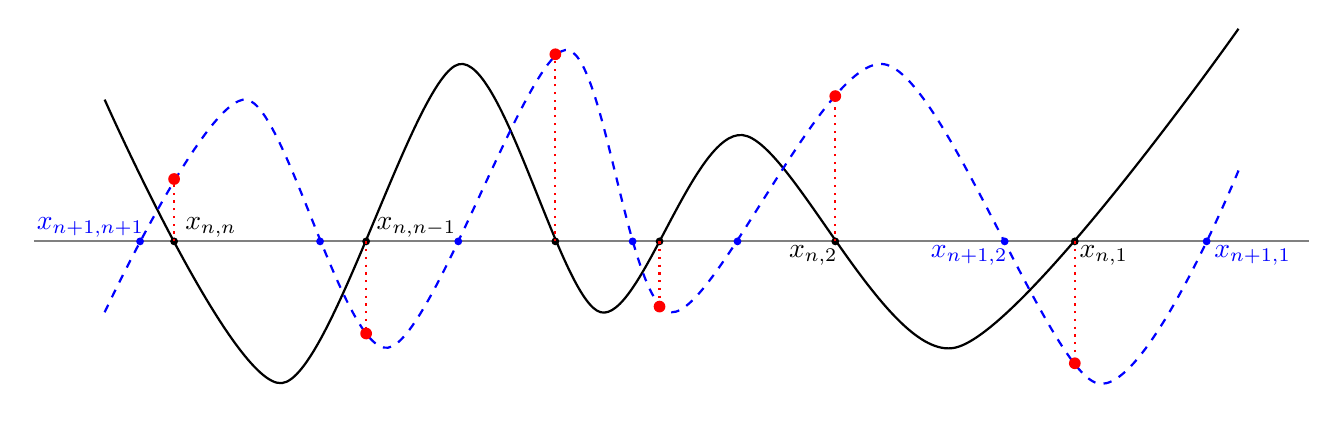
\begin{tikzpicture}[thick,scale=0.9]
  \draw[gray] (-2,0) -- (16,0);
  \draw [black] plot [smooth] coordinates {(-1,2) (1.5,-2) (4,2.5) (6,-1) (8,1.5) (11,-1.5) (15,3)};
  \draw [blue, dashed] plot [smooth] coordinates {(-1,-1) (1,2) (3,-1.5) (5.5,2.7) (7,-1) (10,2.5) (13,-2) (15,1)};
  \node [blue] at (-1.2,.2) {\( x_{n+1,n+1} \)};
  \node [blue] at (15.2,-.2) {\( x_{n+1,1} \)};
  \node [blue] at (11.2,-.2) {\( x_{n+1,2} \)};
  \node at (-.5,0) [blue,circle,fill,inner sep=1pt]{};
  \node at (2.04,0) [blue,circle,fill,inner sep=1pt]{};
  \node at (3.99,0) [blue,circle,fill,inner sep=1pt]{};
  \node at (6.45,0) [blue,circle,fill,inner sep=1pt]{};
  \node at (7.93,0) [blue,circle,fill,inner sep=1pt]{};
  \node at (11.7,0) [blue,circle,fill,inner sep=1pt]{};
  \node at (14.55,0) [blue,circle,fill,inner sep=1pt]{};
  \node at (12.69,0) [circle,fill,inner sep=1pt]{};
  \node at (9.31,0) [circle,fill,inner sep=1pt]{};
  \node at (-.02,0) [circle,fill,inner sep=1pt]{};
  \node at (2.69,0) [circle,fill,inner sep=1pt]{};
  \node at (5.36,0) [circle,fill,inner sep=1pt]{};
  \node at (6.83,0) [circle,fill,inner sep=1pt]{};
  \node at (13.1,-.2) {\( x_{n,1} \)};
  \node at (9.0,-.2) {\( x_{n,2} \)};
  \node at (.5,.2) {\( x_{n,n} \)};
  \node at (3.4,.2) {\( x_{n,n-1} \)};
  \draw [red, dotted] (-.02,0) --++(0,.9);
  \node at (-.02,.88) [red,circle,fill,inner sep=1.5pt]{};
  \draw [red, dotted] (2.69,0) --++(0,-1.3);
  \node at (2.69,-1.3) [red,circle,fill,inner sep=1.5pt]{};
  \draw [red, dotted] (12.69,0) --++(0,-1.72);
  \node at (12.69,-1.72) [red,circle,fill,inner sep=1.5pt]{};
  \draw [red, dotted] (9.31,0) --++(0,2.05);
  \node at (9.31,2.05) [red,circle,fill,inner sep=1.5pt]{};
  \draw [red, dotted] (5.36,0) --++(0,2.64);
  \node at (5.36,2.64) [red,circle,fill,inner sep=1.5pt]{};
  \draw [red, dotted] (6.83,0) --++(0,-0.92);
  \node at (6.83,-0.92) [red,circle,fill,inner sep=1.5pt]{};
\end{tikzpicture}
  \caption{The interchanging zeros of \( P_n(x) \) and \( P_{n+1}(x) \).}
  \label{fig:image2}
\end{figure}
This means that \( P_{n+1}(x) \) has a root between each interval
\( (x_{n,j+1},x_{n,j}) \) for \( j=1,\dots,n-1 \). Considering the
limits \( \lim_{x\to \infty} P_{n+1}(x) = \infty\) and
\( \lim_{x\to -\infty} P_{n+1}(x) = (-1)^{n+1} \infty\), we can see
that \( P_{n+1}(x) \) also has one root in \( (x_{n,1},\infty) \) and
one root in \( (-\infty,x_{n,n}) \). Thus we obtain
\eqref{eq:interlacing}.
\end{proof}

\chapter{Basics of enumerative combinatorics}
\label{cha:basics-enum-comb}

In this chapter we review fundamental objects in enumerative
combinatorics.
From now on we will use the notation \( [n] := \{ 1,\dots,n\} \).

\section{Formal power series and generating functions}

In this section, we study basics of formal power series and generating
functions. See \cite{Wilf2006} for more details on this topic.

A \emph{power series} is a series of the form
\[
 f(x) = a_0 + a_1 x + a_2 x^2 + \cdots.
\]
The quantity \( a_n \) is called the \emph{coefficient of \( x^n \)}
in \( f(x) \). The \emph{constant term} of \( f(x) \) is \( a_0 \),
which we also denote by \( f(0) \).

If the coefficients \( a_n \) are real numbers, then \( f(x) \) may be considered as
a function on \( x \) whose domain is the set of real numbers \( x \)
such that the above infinite series converges. For example, if
\[
  f(x) = 1+x+x^2 + \cdots,
\]
then we have \( f(x) = 1/(1-x) \) for \( |x|<1 \). Thus we can write,
for \( |x|<1 \),
\begin{equation}\label{eq:geometric-series}
  1+x+x^2 + \cdots = \frac{1}{1-x}.
\end{equation}
This, however, does not make sense if \( |x|>1 \). Hence, in calculus,
whenever we consider a power series we always have to mention for what
values of \( x \) the series converges. But in formal power series the
convergence is not needed.

Let \( R \) be a commutative ring with identity. Recall that
\( R[x] \) denotes the ring of polynomials in \( x \) with
coefficients in \( R \).

\begin{defn}
  The \emph{ring of formal power series} in \( x \) with coefficients
  in \( R \) is the set
\[
  R[[x]] = \{a_0 + a_1 x + a_2x^2 + \cdots : a_0,a_1,a_2,\ldots \in R \},
\]
with addition
\[
  \left( \sum_{n=0}^\infty a_n x^n \right) + \left( \sum_{n=0}^\infty
    b_n x^n \right) = \sum_{n=0}^\infty (a_n+b_n) x^n ,
\]
and multiplication
\[
  \left( \sum_{n=0}^\infty a_n x^n \right) \left( \sum_{n=0}^\infty
    b_n x^n \right) = \sum_{n=0}^\infty \left( \sum_{k=0}^n a_k
    b_{n-k} \right)x^n.
\]
\end{defn}

So, roughly speaking, a formal power series is a polynomial of
infinite degree.

The multiplicative identity of \( R[[1]] \) is \( 1 \), that is,
\( 1+0x+0x^2+\cdots \). For \( f(x),g(x) \in R[[1]] \), if
\( f(x) g(x) = 1 \), then we say that \( f(x) \) is the \emph{inverse}
of \( g(x) \) and write \( f(x) = g(x)^{-1} = 1/g(x) \).

In the language of formal power series, \eqref{eq:geometric-series} is
a perfectly valid identity without any convergence considered because
\[
  (1+x+x^2 + \cdots)(1-x) = (1+x+x^2 + \cdots) - x(1+x+x^2 + \cdots) = 1.
\]

An important aspect of formal power series is that the coefficient of
\( x^n \) must be computed using a finitely many additions and
multiplications in \( R \).


\begin{exam}
  The series
\[
  e^{1+x} = \sum_{n\ge 0} \frac{(1+x)^n}{n!}
\]
is not a formal power series in \( \RR[[x]] \) because the constant
term (the coefficient of \( x^0 \)) is \( \sum_{n\ge0} 1/n! \), which
cannot be computed by a finite number of additions and multiplications
in \( \RR \) (although we know \( \sum_{n\ge0} 1/n! = e \)). On the
other hand,
\[
  e\cdot e^{x} = \sum_{n\ge 0} \frac{e x^n}{n!}
\]
is a formal power series in \( \RR[[x]] \). 
\end{exam}

Note that being a formal power series is all about how the series is
presented rather than what values the series take as a function. Most
of the time, we will not consider a formal power series as a function.

For two formal power series \( f(x) = \sum_{n\ge0} f_n x^n \) and
\( g(x) = \sum_{n\ge0} g_n x^n \) with \( g_0=0 \), we define the
\emph{composition} \( (f\circ g)(x) = f(g(x)) \) of \( f(x) \) and
\( g(x) \) by
\begin{equation}\label{eq:12}
  f(g(x)) = \sum_{n\ge0} f_n g(x)^n.
\end{equation}
To see that the above sum is a formal power series, note that since
\( g_0=0 \), every term in \( f_ng(x)^n \) has degree at least
\( n \). Thus, for a fixed \( m\ge0 \), the coefficient of \( x^m \)
in \( f(g(x)) \) is the coefficient of \( x^m \) in the finite sum
\( \sum_{n=0}^m f_n g(x)^n \) of formal power series, which in turn
can be computed in a finite number of additions and multiplications in
\( R \). Note also that if \( g_0\ne 0 \), then the constant term in
the sum \eqref{eq:12} is an infinite sum \( \sum_{n\ge0} f_n g_0 \),
hence \( f(g(x)) \) is not a formal power series (unless \( f(x) \) is
a polynomial).

There is a simple criterion for the existence of an inverse of a
formal power series.

\begin{prop}
  Let \( R \) be a field. A formal power series \( f(x)\in R[[x]] \)
  has an inverse if and only if \( f(0)\ne 0 \).
\end{prop}
\begin{proof}
  (\(\Rightarrow\)) Let \( g(x) \) be the inverse of \( f(x) \).
  Suppose that \( f(0)=0 \). Then the constant term of \( f(x)g(x) \)
  is \( f(0)g(0)=0 \), which is a contradiction to \( f(x)g(x) = 1 \).
  Thus we have \( f(0)\ne 0 \).

  (\(\Leftarrow\)) Let \( f(x) = \sum_{n\ge 0} f_nx^n \).
  Then we can write \( f(x) \) as
  \[
    f(x) = f_0 \left( 1 - h(x) \right),
    \qquad h(x) = \sum_{n\ge 1} h_n x^n, \qquad h_n = - f_0^{-1}f_n.
  \]
  Then the inverse of \( f(x) \) can be found in this way:
  \[
    \frac{1}{f(x)} = \frac{1}{f_0} \cdot \frac{1}{1-h(x)}
    = \frac{1}{f_0} \sum_{n\ge0} h(x)^n.
  \]
  Since the lowest degree term of \( h(x)^n \) has degree at least \( n \),
  the above infinite sum is a well-defined formal power series.
\end{proof}

As in calculus we define the \emph{derivative} of a formal power
series \( f(x) = \sum_{n\ge0} f_n x^n \) by
\[
  f'(x) := \sum_{n\ge1} n f_n x^{n-1} = \sum_{n\ge0} (n+1) f_{n+1} x^{n}.
\]
The usual differentiation rules hold.
\begin{prop}
  For two formal power series \( f(x) \) and \( g(x) \),
  we have
\begin{align*}
  (f(x)g(x))'
  &= f'(x) g(x) + f(x) g'(x), \\
  \left(\frac{f(x)}{g(x)}\right)'
  &= \frac{f'(x) g(x) - f(x) g'(x)}{g(x)^2}, \qquad g(x) \ne 0,\\
  (f(g(x)))'
  &= f'(g(x)) g'(x), \qquad g(0) = 0.
\end{align*}
\end{prop}

\begin{proof}
  We can prove these identities using the formal definition of the
  derivative. We will only proof the first identity. Let
  \( f(x) = \sum_{n\ge0} f_n x^n \) and
  \( g(x) = \sum_{n\ge0} g_n x^n \). Then
  \[
    (f(x)g(x))' = \left( \sum_{n\ge 0} \left( \sum_{k=0}^{n} f_kg_{n-k} \right) x^{n} \right)'
      = \sum_{n\ge 0} \left( \sum_{k=0}^{n} n f_kg_{n-k}
    \right) x^{n-1}.
  \]
  On the other hand,
  \begin{align*}
    f'(x) g(x) + f(x) g'(x)
    & =  \sum_{n\ge0} n f_n x^{n-1} \sum_{n\ge0} g_n x^n +   
      \sum_{n\ge0} f_n x^n \sum_{n\ge0} n g_n x^{n-1}\\
    &= \sum_{n\ge 0} \left( \sum_{k=0}^{n} kf_kg_{n-k}
      + \sum_{k=0}^{n} f_k\cdot (n-k)g_{n-k} \right) x^{n-1}\\
    &= \sum_{n\ge 0} \left( \sum_{k=0}^{n} nf_kg_{n-k} \right) x^{n-1}.
  \end{align*}
  Thus we get the first identity.
\end{proof}





We can naturally extend the definition of formal power series to the
multivariate case.


\begin{defn}
  Let \( \vx =(x_1,x_2,\dots) \) be a sequence of variables. Let
  \( Z \) denote the set of sequences
  \( I=(i_1,i_2,\dots)\in \ZZ_{\ge0}^\infty \) such that
  \( i_1+i_2 + \cdots < \infty \). For \( I=(i_1,i_2,\dots)\in Z \),
  we write \( \vx^I = x_1^{i_1} x_2^{i_2} \cdots \). The \emph{ring of
    formal power series} in \( x_1,x_2,\dots \) with coefficients in
  \( R \) is the set
\[
  R[[\vx]] = \left\{ \sum_{I\in Z} a_I \vx^I  : a_I\in R \right\},
\]
with addition
\[
  \left(\sum_{I\in Z} a_I \vx^I \right) + \left(\sum_{I\in Z} b_I \vx^I
  \right) = \left( \sum_{I\in Z} (a_I+b_I) \vx^I \right),
\]
and multiplication
\[
  \left(\sum_{I\in Z} a_I \vx^I \right) \left(\sum_{I\in Z} b_I \vx^I
  \right) = \sum_{I\in Z} \left( \sum_{I_1,I_2\in Z, I_1+I_2=I} a_{I_1} b_{I_2} \right) \vx^I.
\]
\end{defn}

Again, rougly speaking, a multivariate formal power series is a
multivariate polynomial of infinite degree.


Now we define the notion of generating functions.


\begin{defn}
  The \emph{generating function} for a sequences \( \{ a_n\}_{n\ge 0} \) is
  defined to be the formal power series
\[
  a_0 + a_1 x + a_2 x^2 + \cdots.
\]
\end{defn}

So, the generating function for \( \{ a_n\}_{n\ge 0} \) is nothing but
a way of recording the sequence. One of the benefits of generating
functions is that we can use many properties of formal power series.


\begin{exam}
  The generating function for \( \{ a_n = 2^n\}_{n\ge 0} \) is
  \begin{equation}\label{eq:15}
    \sum_{n\ge 0} 2^n x^n = \sum_{n\ge 0} (2x)^n = \frac{1}{1-2x}.
  \end{equation}
\end{exam}

\begin{exam}
  Let's find the generating function for \( \{ a_n = n 2^n\}_{n\ge 0} \).
  Differentiating both sides of \eqref{eq:15}, we get
  \[
    \sum_{n\ge 0} n2^n x^{n-1} =  \frac{2}{(1-2x)^2}.
  \]
  Multiplying both sides by \( x \), we obtain
  \[
    \sum_{n\ge 0} n2^n x^{n} =  \frac{2x}{(1-2x)^2}.
  \]
\end{exam}

We can easily extend the definition of generating functions to
accommodate arrays \( \{ a_I\}_{I\in Z} \) of elements \( a_I\in R \)
using multivariate formal power series. More generally, we will
consider generating functions for arbitrary (combinatorial) objects.

\begin{defn}
  Let \( A \) be a set of objects. A \emph{weight} on \( A \) is a
  function \( \wt:A\to R \), where \( R \) is any commutative ring.
  The \emph{generating function} for \( A \) with respect to the
  weight function \( \wt \) is the formal power series
  \[
    \sum_{a \in A} \wt(a).
  \]
\end{defn}



\begin{exam}
  Let \( A = \{0,1,2,\dots\} \) and define a weight of \( A \) by
  \( \wt(a) = x^a \). Then the generating function for \( A \)
  (with this weight) is
  \[
    \sum_{a \in A} \wt(a) = \sum_{n=0}^n \wt(n)
    = \sum_{n=0}^n x^n = \frac{1}{1-x}.
  \]
\end{exam}

\begin{exam}
  Let \( A \) be the set of subsets of \( [n] \) and define a weight
  of \( A \) by \( \wt(a) = x^{|a|}y^{n-|a|} \). Then the generating function for
  \( A \) (with this weight) is
  \[
    \sum_{a \in A} \wt(a) = \sum_{a\subseteq [n]} x^{|a|} y^{n-|a|} =
    \sum_{k=0}^n \binom{n}{k} x^{k}y^{n-k} = (x+y)^n.
  \]
\end{exam}

\begin{exam}
  Let \( A \) be the set \( S_n \) of permutations of \( [n] \) and
  define a weight of \( A \) by \( \wt(a) = x^{\cycle(a)} \). Then it
  can be proved (see \eqref{eq:c(n,k)-gf}) that the generating
  function for \( A \) (with this weight) is
  \[
    \sum_{a \in A} \wt(a) = \sum_{\pi\in S_n} x^{\cycle(a)} = x(x+1)
    \cdots (x+n-1).
  \]
\end{exam}

We will often use the term ``generating function'' in a flexible
manner. For example, the generating function for the number of
permutations would mean the generating function for the sequence
\( \{a_n = n!\}_{n\ge0} \), that is, \( \sum_{n\ge0} n! x^n \).

\section{Dyck paths and Motzkin paths}

In this section we introduce two important classes of lattice paths.
These are fundamental objects in studying orthogonal polynomials
combinatorially.


\begin{defn}
  A \emph{lattice path} from \( u \) to \( v \) is a sequence
  \( \pi = (v_0,v_1,\dots,v_n) \) of points in \( \ZZ\times\ZZ \) with
  \( v_0=u \) and \( v_n =v \). Each pair \( (v_i,v_{i+1}) \) of
  consequence points is called a \emph{step} of \( \pi \). 
\end{defn}

A path \( \pi = (v_0,v_1,\dots,v_n) \) is also considerd as a sequence
\( S_1 \cdots S_n \) of steps, where \( S_i=(v_{i-1},v_i) \). We will
sometimes identify a step \( (v_i,v_{i+1}) \) with
\( v_{i+1} - v_i \in \ZZ\times\ZZ \).

\begin{defn}
  A \emph{Dyck path} is a lattice path consisting of \emph{up steps}
  \( (1,1) \) and \emph{down steps} \( (1,-1) \) that stays on or
  above the \( x \)-axis, see \Cref{fig:dyck-path}. Denote by
  \( \Dyck(u\to v) \) the set of Dyck paths from \( u \) to \( v \).
  We also define \( \Dyck_{2n} = \Dyck((0,0)\to (2n,0))\).
\end{defn}

\begin{figure}
  \centering
  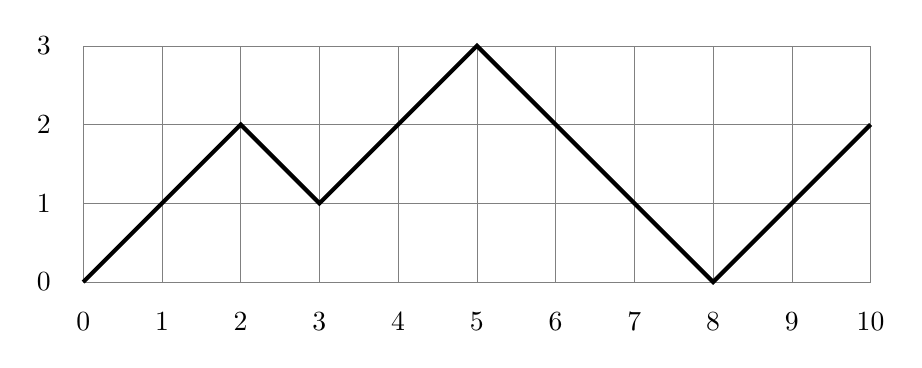
\begin{tikzpicture}
      \draw[help lines] (0,0) grid (10,3);
\foreach \x in {0,...,10} \draw node at (\x,-.5) {\( \x \)};
\foreach \y in {0,...,3} \draw node at (-.5,\y) {\( \y \)};
\draw[line width = 1.5pt] (0,0) -- ++(1,1) -- ++(1,1) -- ++(1,-1) -- ++(1,1) -- ++(1,1) -- ++(1,-1) -- ++(1,-1) -- ++(1,-1) -- ++(1,1) -- ++(1,1);
  \end{tikzpicture}
  \caption{A Dyck path from \( (0,0) \) to \( (10,2) \).}
  \label{fig:dyck-path}
\end{figure}



Let's enumerate the Dyck paths in \( \Dyck_{2n} \) using generating
functions. To do this let
\[
  C(x) = \sum_{n\ge 0} |\Dyck_{2n}| x^n.
\]
Then
we can also write
\[
  C(x) = \sum_{\pi\in \Dyck} \wt(\pi),
\]
where \( \Dyck \) is the set of all Dyck paths from \( (0,0) \) to
\( (2n,0) \) for some \( n\ge0 \) and \( \wt(\pi) = x^{d(\pi)} \),
where \( d(\pi) \) is the number of down steps in \( \pi \). It is
helpful to imagine the generating function \( C(x) \) as a picture of
all Dyck paths, where each Dyck path has its weight attached to it as
shown in \Cref{fig:gf-dyck}.

\begin{figure}
  \centering
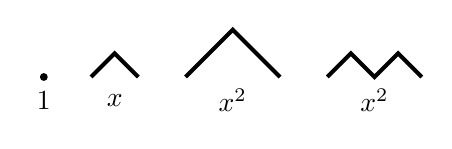
\begin{tikzpicture}[scale=0.3]
\node at (0,0) [circle,fill,inner sep=1pt]{};
\draw[line width = 1.5pt] (2,0) -- ++(1,1) -- ++(1,-1);
\draw[line width = 1.5pt] (6,0) -- ++(1,1) -- ++(1,1) -- ++(1,-1) -- ++(1,-1);
\draw[line width = 1.5pt] (12,0) -- ++(1,1) -- ++(1,-1) -- ++(1,1) -- ++(1,-1);
\node at (0,-1) {\( 1 \)};
\node at (3,-1) {\( x \)};
\node at (8,-1) {\( x^2 \)};
\node at (14,-1) {\( x^2 \)};
\end{tikzpicture}
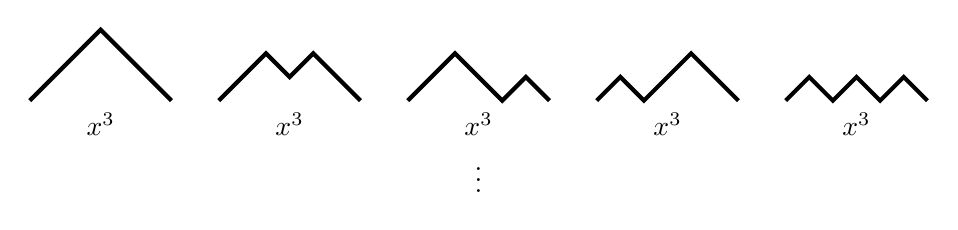
\begin{tikzpicture}[scale=0.3]
\draw[line width = 1.5pt] (0,0) -- ++(1,1) -- ++(1,1) -- ++(1,1) -- ++(1,-1) -- ++(1,-1) -- ++(1,-1);
\draw[line width = 1.5pt] (8,0) -- ++(1,1) -- ++(1,1) -- ++(1,-1) -- ++(1,1) -- ++(1,-1) -- ++(1,-1);
\draw[line width = 1.5pt] (16,0) -- ++(1,1) -- ++(1,1) -- ++(1,-1) -- ++(1,-1) -- ++(1,1) -- ++(1,-1);
\draw[line width = 1.5pt] (24,0) -- ++(1,1) -- ++(1,-1) -- ++(1,1) -- ++(1,1) -- ++(1,-1) -- ++(1,-1);
\draw[line width = 1.5pt] (32,0) -- ++(1,1) -- ++(1,-1) -- ++(1,1) -- ++(1,-1) -- ++(1,1) -- ++(1,-1);
\node at (3,-1) {\( x^3 \)};
\node at (11,-1) {\( x^3 \)};
\node at (19,-1) {\( x^3 \)};
\node at (27,-1) {\( x^3 \)};
\node at (35,-1) {\( x^3 \)};
\node at (19,-3) {\( \vdots \)};
\end{tikzpicture}
  \caption{An illustration of the generating function for Dyck paths.}
  \label{fig:gf-dyck}
\end{figure}


\begin{figure}
  \centering
  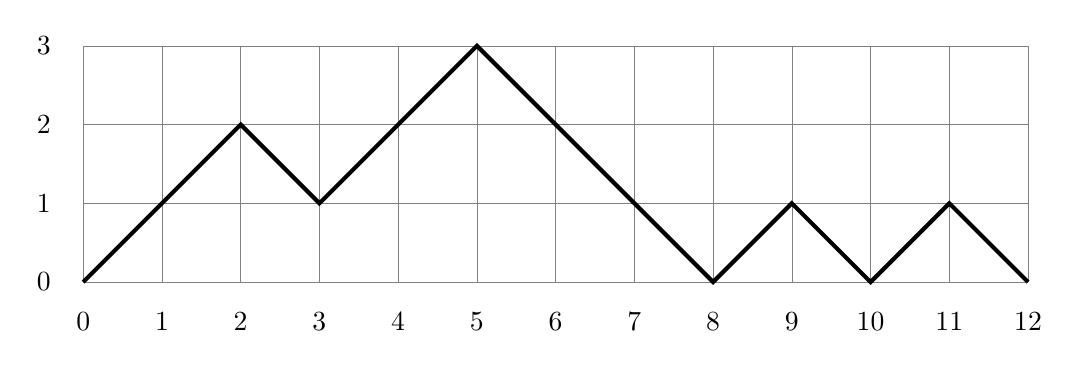
\begin{tikzpicture}
    \draw[help lines] (0,0) grid (12,3);
\foreach \x in {0,...,12} \draw node at (\x,-.5) {\( \x \)};
\foreach \y in {0,...,3} \draw node at (-.5,\y) {\( \y \)};
\draw[line width = 1.5pt] (0,0) -- ++(1,1) -- ++(1,1) -- ++(1,-1) -- ++(1,1) -- ++(1,1) -- ++(1,-1) -- ++(1,-1) -- ++(1,-1) -- ++(1,1) -- ++(1,-1) -- ++(1,1) -- ++(1,-1);
  \end{tikzpicture}
  \caption{A Dyck path \( \pi \) from \( (0,0) \) to \( (12,0) \).}
  \label{fig:dyck-path2}
\end{figure}

A Dyck path \( \pi \in \Dyck \) can be considered as a sequence of up
steps and down steps. For example, the Dyck path in
\Cref{fig:dyck-path2} is \( \pi = UUDUUDDDUDUD \). Every nonempty Dyck
path \( \pi \in \Dyck \) is uniquely decomposed into
\( \pi = U \tau D \rho \) for some \( \tau,\rho\in \Dyck \). For our
running example,
\begin{equation}\label{eq:dyck-decomp}
  \pi=UUDUUDDDUDUD = U(UDUUDDD)(UDUD),
\end{equation}
so we have
\( \tau = UDUUDDD \) and \( \rho = UDUD \).
This argument shows that
\begin{equation}\label{eq:cat-gf}
  C(x) = 1 + C(x) x C(x).
\end{equation}
Solving this quadratic equation for \( C(x) \), we
get
\begin{equation}\label{eq:16}
   C(x)  = \frac{1\pm\sqrt{1-4x}}{2x}.
  \end{equation}

  We must choose the correct sign here. First, by setting \( x=0 \),
  we obtain that the constant term of \( \sqrt{1-4x} \) is \( 1 \).
  Thus \eqref{eq:16} is a valid formal power series only for the minus
  sign. This implies that
  \[
    \sum_{n\ge0} |\Dyck_{2n}| x^n = \frac{1-\sqrt{1-4x}}{2x}.
  \]
 
  Now we can use the \emph{binomial theorem}
\[
  (1+x)^\alpha := \sum_{n\ge 0} \binom{\alpha}{n} x^n,
\]
where
\[
  \binom{\alpha}{n} = \frac{\alpha(\alpha-1)\cdots (\alpha-n+1)}{n!}.
\]
By the binomial theorem, we have
  \begin{align*}
    \sqrt{1-4x}
    &= (1-4x)^{1/2} = \sum_{n\ge 0} \binom{1/2}{n} (-4x)^n
    = 1+ \sum_{n\ge 1} \frac{\frac{1}{2} \frac{-1}{2}
    \frac{-3}{2} \cdots \frac{-2n+3}{2}}{n!} (-1)^n 4^n x^n\\
    &= 1- \sum_{n\ge 1} \frac{1\cdot 3\cdot \cdots \cdot (2n-3)}{n!} 2^n x^n
    = 1- \sum_{n\ge 1} \frac{2(2n-2)!}{n!(n-1)!} x^n .
  \end{align*}
  Therefore,
  \[
   \sum_{n\ge0} |\Dyck_{2n}| x^n = \frac{1-\sqrt{1-4x}}{2x} 
   = \sum_{n\ge 1} \frac{1}{n} \binom{2n-2}{n-1} x^{n-1}
   = \sum_{n\ge 0} \frac{1}{n+1} \binom{2n}{n} x^n.
  \]
  Comparing the coefficient of \( x^n \) in both sides we obtain the
  following result.

\begin{prop}
  We have
  \begin{equation}\label{eq:17}
    |\Dyck_{2n}| = \frac{1}{n+1} \binom{2n}{n}.
  \end{equation}
\end{prop}
Note that we proved \eqref{eq:17} using generating functions, but this
can also be proved by a standard reflection principle.

The \emph{Catalan number} \( C_n \) is defined by
\[
  C_n = \frac{1}{n+1} \binom{2n}{n}.
\]
The first few Catalan numbers are
\[
  1, 1, 2, 5, 14, 42, 132, 429, 1430, 4862, \ldots.
\]

There are many combinatorial objects counted by the Catalan number.
Stanley \cite{Stanley2015} collected more than 200 such ``Catalan
objects''. Dyck paths are one of the most well-known Catalan objects.
Some of other well known Catalan objects are triangulations of an
\( (n+2) \)-gon, ballot sequences of length \( 2n \), and plane binary
trees with \( n \) vertices.

The Catalan numbers satisfy the following recurrence:
\begin{equation}\label{eq:cat-rec}
  C_0 = 1, \qquad
  C_n = \sum_{k=0}^{n} C_k C_{n-1-k}, \qquad n\ge1.
\end{equation}
This recurrence can be proved similarly as \eqref{eq:cat-gf} using the
decomposition \eqref{eq:dyck-decomp}.


Now we consider lattice paths with three kinds of steps. These lattice
paths will play a fundamental role in Viennot's theory of orthogonal
polynomials.

\begin{defn}
  A \emph{Motzkin path} is a lattice path consisting of \emph{up
    steps} \( (1,1) \), \emph{horizontal steps} \( (1,0) \), and
  \emph{down steps} \( (1,-1) \) that stays on or above the
  \( x \)-axis, see Figure~\ref{fig:motzkin}. Denote by
  \( \Motz(u\to v) \) the set of Dyck paths from \( u \) to \( v \).
  We also define \( \Motz_{n} = \Motz((0,0)\to (n,0))\).
\end{defn}

\begin{figure}
  \centering
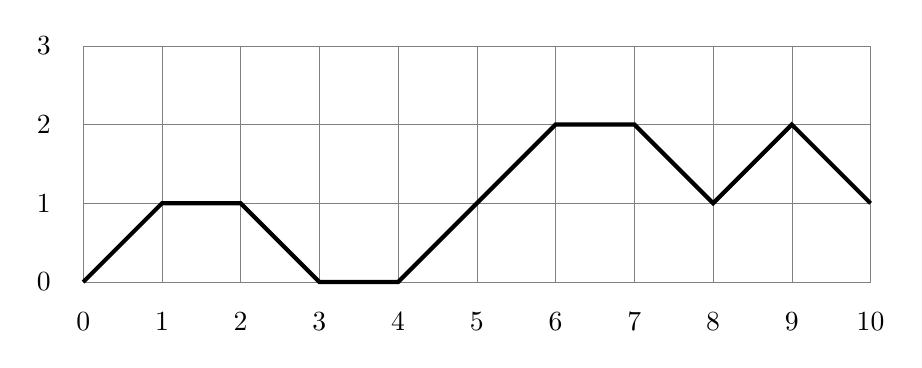
\begin{tikzpicture}
  \draw[help lines] (0,0) grid (10,3);
\foreach \x in {0,...,10} \draw node at (\x,-.5) {\( \x \)};
\foreach \y in {0,...,3} \draw node at (-.5,\y) {\( \y \)};
\draw[line width = 1.5pt] (0,0) -- ++(1,1) -- ++(1,0) -- ++(1,-1) -- ++(1,0) -- ++(1,1) -- ++(1,1) -- ++(1,0) -- ++(1,-1) -- ++(1,1) -- ++(1,-1);
\end{tikzpicture}
\caption{A Motzkin path from \( (0,0) \) to \( (10,1) \).}
  \label{fig:motzkin}
\end{figure}

Considering the positions of horizontal steps, we can relate the
number of Motzkin paths and that of Dyck paths.



\begin{prop}
  We have
  \[
    |\Motz_{n}| = \sum_{k=0}^{\flr{n/2}} \binom{n}{2k} C_k.
  \]
\end{prop}

\begin{prop}
  Let \( M(x) = \sum_{n\ge 0} |\Motz_n| x^n \). Then
  \[
    M(x) = \frac{1-x-\sqrt{1-2x-3x^2}}{2x^2}.
  \]
\end{prop}
\begin{proof}
  By a similar argument used to prove  \eqref{eq:cat-gf},
  we have
  \[
    M(x) = 1 + x M(x) + M(x) x^2 M(x).
  \]
  Solving the equation we obtain the desired formula.
\end{proof}


\section{Set partitions and matchings}

In this section we study set partitions and matchings. They will be
used to give combinatorial interpretations for moments of Charlier
polynomials and Hermite polynomials.

\begin{defn}
  A \emph{set partition} of a set \( X \) is a collection
  \( \pi = \{B_1,\dots,B_k\} \) of subsets of \( X \)
  such that
  \begin{enumerate}
  \item \( B_i\ne\emptyset \) for all \( i \),
  \item \( B_i\cap B_j = \emptyset \) for all \( i\ne j \), and
  \item \( B_1 \cup \cdots \cup B_k = X \).
  \end{enumerate}
  Each \( B_i \) is called a \emph{block} of \( \pi \).
\end{defn}

A set partition can be visualized by connecting consecutive elements
in each block see \Cref{fig:set-partition}.

\begin{figure}
  \centering
  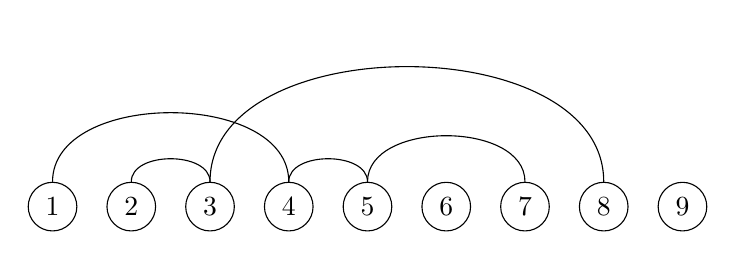
\begin{tikzpicture}
    \begin{scope}[shift={(0,0)}]
\node[draw, circle] (1) at (1,0) {\( 1 \)};
\node[draw, circle] (4) at (4,0) {\( 4 \)};
\node[draw, circle] (5) at (5,0) {\( 5 \)};
\node[draw, circle] (7) at (7,0) {\( 7 \)};
\draw[out=90,in=90] (1) to (4);
\draw[out=90,in=90] (4) to (5);
\draw[out=90,in=90] (5) to (7);
\node[draw, circle] (2) at (2,0) {\( 2 \)};
\node[draw, circle] (3) at (3,0) {\( 3 \)};
\node[draw, circle] (8) at (8,0) {\( 8 \)};
\draw[out=90,in=90] (2) to (3);
\draw[out=90,in=90] (3) to (8);
\node[draw, circle] (6) at (6,0) {\( 6 \)};
\node[draw, circle] (9) at (9,0) {\( 9 \)};
\end{scope}
\end{tikzpicture}
\caption{A visualization of a set partition
  \( \{\{1,4,5,7\}, \{2,3,8\}, \{6\}, \{9\}\} \) of \( [9] \).}
\label{fig:set-partition}
\end{figure}

We denote by \( \Pi_n \) the set of all set partitions of \( [n] \).
We also define \( \Pi_{n,k} \) to be the set of all set partitions of
\( [n] \) with exactly \( k \) blocks. The \emph{Stirling number of
  the second kind} \( S(n,k) \) is the cardinality of \( \Pi_{n,k} \).

We use the convention that \( \emptyset \) is the only set partition
of \( \emptyset \), i.e., \( \Pi_0 = \{\emptyset\} \). The following
are immediate from the definition of set partitions:
\begin{itemize}
\item \( S(n,0) = \delta_{n,0} \),
\item \( S(n,n) = 1 \),
\item \( S(n,k) = 0 \) if \( k>n \).
\end{itemize}

We can compute the number \( S(n,k) \) using the following recursion
with the above initial conditions.

\begin{prop}
  For integers \( n,k\ge1 \), we have
  \[
    S(n,k) = S(n-1,k-1) + k S(n-1,k).
  \]
\end{prop}
\begin{proof}
  Let \( \pi\in \Pi_{n,k} \). If \( n \) is in a singleton of
  \( \pi \), then \( \pi\setminus\{n\} \in \Pi_{n-1,k-1} \). Otherwise,
  \( \pi \) can be obtained from a set partition
  \( \pi'\in \Pi_{n-1,k} \) by adding \( n \) to one of the \( k \)
  blocks of \( \pi' \). This shows the recursion.
\end{proof}


\begin{prop}
  We have
  \[
    S(n,k) = \frac{1}{k!} \sum_{i=0}^{k} (-1)^{k-i} \binom{k}{i}i^n.
  \]
\end{prop}

\begin{proof}
  The number of onto functions \( f:[n] \to [k] \) is \( k! S(n,k) \).
  By the principle of inclusion and exclusion, this number is equal to
  \[
     k! S(n,k) = \sum_{i=0}^{k} (-1)^{k-i} \binom{k}{i}i^n,
  \]
  which implies the desired formula.
\end{proof}

For an integer \( n\ge0 \), a \emph{falling factorial} \( (x)_n \) is defined by
\[
  (x)_n = x(x-1) \cdots (x-n+1).
\]

\begin{prop}
  We have
  \begin{equation}\label{eq:S(n,k)(x)k=xn}
    \sum_{k=0}^{n} S(n,k) (x)_k = x^n.
  \end{equation}
\end{prop}

\begin{proof}
  Since both sides are polynomials in \( x \), it suffices to show
  that the identity holds for all positive integers \( x \). So, let's
  assume that \( x \) is a positive integer. Then the right-hand side
  is the number of all functions \( f: [n] \to [x] \).

  Now, consider a function \( f: [n] \to [x] \) such that the image
  \( f([n]) \) has exactly \( k \) elements. Let
  \( f([n]) = \{a_1<\dots<a_k\} \). Then
  \( \{f^{-1}(a_1),\dots,f^{-1}(a_k)\} \) is a set partition of
  \( [n] \) with \( k \) blocks. Thus such a function \( f \) is
  obtained by first partitionining \( [n] \) into \( k \) blocks
  \( B_1,\dots,B_k \) and constructing a one-to-one map from
  \( \{B_1,\dots,B_k\} \) to \( [x] \). This shows that the number of
  such functions is \( S(n,k) (x)_k \). Summing over all \( k \) gives
  the number of all functions \( f: [n] \to [x] \).

  Since both sides of the identity count the same number, they are
  equal.
\end{proof}

\begin{defn}
  A \emph{matching} on a set \( X \) is a set partition
  \( \pi = \{B_1,\dots,B_k\} \) of \( X \) in which every block has
  size \( 1 \) or \( 2 \). Each block of size \( 1 \) is called a
  \emph{fixed point} and each block of size \( 2 \) is called an
  \emph{edge} or an \emph{arc} of \( \pi \).
\end{defn}

A matching is said to be \emph{perfect} or \emph{complete} if there
are no fixed points.

\begin{prop}
  The number of complete matchings of \( [2n] \) is
  \[
    (2n-1)!! := 1 \cdot 3 \cdot \cdots \cdot (2n-1).
  \]
  The number of matchings of \( [n] \) is
  \[
    \sum_{k=0}^{\flr{n/2}} \binom{n}{2k} (2k-1)!!.
  \]
\end{prop}

\begin{proof}
  The first identity can easily be proved by induction on \( n \)
  since there are \( 2n-1 \) ways to form an edge with the last
  element \( 2n \) and another element.

  The second identity follows from the observation that if a matching
  of \( [n] \) has \( k \) edges, then these edges form a complete
  matching on a set of size \( 2k \).
\end{proof}

\section{Permutations}

In this section we study permutations, which are one of the most
fundamental objects in combinatorics. We will see later a connection
between permutations and moments of Laguerre polynomials.

\begin{defn}
  A \emph{permutation} on \( [n] \) is a bijection
  \( \pi:[n] \to [n] \). The \emph{symmetric group} \( \sym_n \) is
  the group of permutations on \( [n] \) with multiplication given by
  composition of functions.
\end{defn}

For \( \pi,\tau\in \sym_n \), we write \( \pi\tau = \pi\circ \tau \),
that is \( \pi\tau \) is the permutation defined by
\( (\pi\tau)(i) = \pi(\tau(i)) \).

Let \( \pi:[n] \to [n] \) be a permutation. We will often write
\( \pi_i = \pi(i) \) and identify this permutation with a word
\[
  \pi = \pi_1\pi_2 \cdots \pi_n,
\]
which is called the \emph{one-line notation} of \( \pi \). The
\emph{two-line notation} of \( \pi \) is the array
\[
\pi = \begin{pmatrix}
1 & 2 & \cdots & n\\
\pi_1 & \pi_2 & \cdots & \pi_n
\end{pmatrix}.
\]

\begin{exam}
  Let \( \pi\in\sym_3 \) be the permutation given by
  \[
    \pi(1) = 2, \pi(2) = 3, \pi(3) =1.
  \]
  Then in one-line notation,
  \[
    \pi = \pi_1\pi_2\pi_3 = 2 3 1
  \]
  and in two-line notation,
  \[
    \pi =
    \begin{pmatrix}
1 & 2 & 3\\
2 & 3 & 1
\end{pmatrix}.
  \]
  We have
  \[
    \pi^2 =
    \begin{pmatrix}
1 & 2 & 3\\
3 & 1 & 2
    \end{pmatrix}, \qquad
        \pi^3 =
    \begin{pmatrix}
1 & 2 & 3\\
1 & 2 & 3
    \end{pmatrix}.
  \]
\end{exam}


A \emph{cycle} of \( \pi \) is a sequence \( (a_1,\dots,a_k) \) of
distinct elements of \( [n] \) such that
\[
  \pi(a_1) = a_2, \qquad  
  \pi(a_2) = a_3, \qquad 
  \ldots, \qquad 
  \pi(a_k) = a_1.
\]
We denote by \( \cycle(\pi) \) the number of cycles in \( \pi \).

A cycle \( (a_1,\dots,a_k) \) is considered to be the same as any of
its \emph{cyclic shift} \( (a_j,\dots, a_k, a_1, \dots,a_{j-1}) \). We
also consider a cycle \( \rho=(a_1,\dots,a_k) \) as a permutation of
\( [n] \) such that
\[
  \rho(i) =
  \begin{cases}
   i & \mbox{if \( i\not\in \{a_1,\dots,a_k\} \)},\\
    a_{j+1} & \mbox{if \( i=a_j \),}
  \end{cases}
\]
where \( a_{k+1} = a_1 \).

A \emph{cycle of length \( k \)} is a permutation (in some
\( \sym_n \)) of the form \( (a_1,\dots,a_k) \). A
\emph{transposition} is a cycle of length \( 2 \). A \emph{simple
  transposition} is a transposition of the form \( (i,i+1) \).

Note that for a permutation \( \pi = \pi_1 \cdots \pi_n \in \sym_n \)
and a transposition \( \tau = (i,j)\in \sym_n \) with \( i<j \), the
product \( \pi\tau \) is the permutation obtained from \( \pi \)
by interchaning the values \( \pi_i \) and \( \pi_j \) at the
positions \( i \) and \( j \):
\[
  \pi\tau = \pi_1 \cdots \pi_{i-1} \pi_j \pi_{i+1} \cdots \pi_{j-1}
  \pi_i \pi_{j+1} \cdots \pi_n.
\]
On the other hand, the product \( \tau\pi \) is the permutation
obtained from \( \pi \) by interchaning the values \( i \) and
\( j \). For example, if \( \pi = \cdots i \cdots j \cdots \), then
\( \tau\pi = \cdots j \cdots i \cdots \).


\begin{prop}\label{pro:cycle-decomp}
  Let \( \pi \in \sym_n \). Then we can write
  \( \pi = \rho_1 \cdots \rho_k \) for some disjoint cycles
  \( \rho_1,\dots,\rho_k \) in \( \sym_n \). Moreover, we can also
  write \( \pi = s_1 \cdots s_r \) for some (not necessarily disjoint)
  simple transpositions \( s_i\in \sym_n \).
\end{prop}
\begin{proof}
  Let \( \pi\in \sym_n \). Let \( m=1 \) and consider the sequence
  \( \pi(m), \pi^2(m), \ldots \). Since this is an infinite sequence
  of integers in \( [n] \), we must have \( \pi^i(m) = \pi^j(m) \) for
  some \( i<j \). By multiplying \( \pi^{-i} \), we have
  \( m = \pi^{j-i}(m) \). Thus we can find the smallest integer
  \( r \) such that \( \pi^r(m) = m \). Let \( \rho_1 \) be the cycle
  \( (k,\pi(k), \pi^2(k),\dots,\pi^{r-1}(k)) \).

  Now let \( m \) be the smallest integer in \( [n] \) except those in
  \( \rho_1 \). We repeat this process and obtain cycles
  \( \rho_1,\dots,\rho_k \) whose union as a set is \( [n] \). These
  cycles are disjoint because if \( \rho_i \) and \( \rho_j \) have a
  common element then they must be the same cycle.

  For the second statement, let \( \pi=\pi_1 \cdots \pi_n \). Note
  that multiplying a simple transposition \( (i,i+1) \) on the left of
  \( \pi \) interchanges \( \pi_i \) and \( \pi_{i+1} \). Thus we can
  sort \( \pi=\pi_1 \cdots \pi_n \) into the the identity permutation
  \( 1 2 \cdots n \) by multiplying simple transpositions
  \( t_1, \ldots, t_r \) on the left, i.e.,
  \( \pi t_1 \cdots t_r = id \). Then \( \pi = t_r \cdots t_1 \),
  which is a product of simple transpositions.
\end{proof}


By \Cref{pro:cycle-decomp}, we can write \( \pi \) in \emph{cycle
  notation}, i.e., as a product of its disjoint cycles:
\[
  \pi = \rho_1 \cdots \rho_r.
\]

\begin{exam}
  Let \( \pi = 951826743 \in \sym_9 \).
  In two-line notation,
  \[
    \pi =
\begin{pmatrix}
1 & 2 & 3 & 4 & 5 & 6 & 7 & 8 & 9\\
9 & 5 & 1 & 8 & 2 & 6 & 7 & 4 & 3
\end{pmatrix}.
  \]
  There are 5 disjoint cycles of \( \pi \), namely, \( (1,9,3) \),
  \( (2,5) \), \( (4,8) \), \( (6) \), and \( (7) \). Thus, in cycle
  notation,
  \[
    \pi = (1,9,3)(2,5)(4,8) (6) (7).
  \]
  Thus, \( \cycle(\pi) = 5 \). We sometime omit the cycles of length
  \( 1 \) and write
  \[
    \pi = (1,9,3)(2,5)(4,8).
  \]
\end{exam}

We can also visualize a permutation by drawing its cycles as shown in
\Cref{fig:cycle}.

\begin{figure}
  \centering
  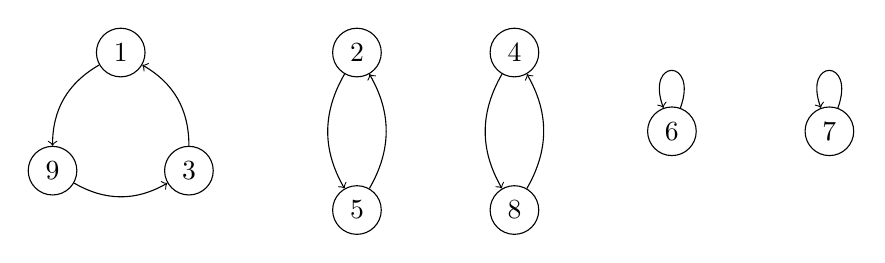
\begin{tikzpicture}
    \begin{scope}[shift={(0,0)}]
\node[draw, circle] (0) at ({90 + (360/3 * 0)}:1) {\( 1 \)};
\node[draw, circle] (1) at ({90 + (360/3 * 1)}:1) {\( 9 \)};
\node[draw, circle] (2) at ({90 + (360/3 * 2)}:1) {\( 3 \)};
\draw[->,bend right] (0) to (1);
\draw[->,bend right] (1) to (2);
\draw[->,bend right] (2) to (0);
\end{scope}
\begin{scope}[shift={(3,0)}]
\node[draw, circle] (0) at ({90 + (360/2 * 0)}:1) {\( 2 \)};
\node[draw, circle] (1) at ({90 + (360/2 * 1)}:1) {\( 5 \)};
\draw[->,bend right] (0) to (1);
\draw[->,bend right] (1) to (0);
\end{scope}
\begin{scope}[shift={(5,0)}]
\node[draw, circle] (0) at ({90 + (360/2 * 0)}:1) {\( 4 \)};
\node[draw, circle] (1) at ({90 + (360/2 * 1)}:1) {\( 8 \)};
\draw[->,bend right] (0) to (1);
\draw[->,bend right] (1) to (0);
\end{scope}
\begin{scope}[shift={(7,-1)}]
\node[draw, circle] (0) at ({90 + (360/1 * 0)}:1) {\( 6 \)};
\draw[->,out=70,in=110,looseness=8] (0) to (0);
\end{scope}
\begin{scope}[shift={(9,-1)}]
\node[draw, circle] (0) at ({90 + (360/1 * 0)}:1) {\( 7 \)};
\draw[->,out=70,in=110,looseness=8] (0) to (0);
\end{scope}
  \end{tikzpicture}
  \caption{A visualization of a permutation
    \( \pi = (1,9,3)(2,5)(4,8) (6) (7) \in \sym_9 \).}
  \label{fig:cycle}
\end{figure}


\begin{defn}
  A permutation \( \pi\in \sym_n \) is called an \emph{involution} if
  \( \pi^2 = \iota \), where \( \iota \) is the identity permutation
  on \( [n] \). Let \( \invol_n \) denote the set of involutions in
  \( \sym_n \).
\end{defn}

\begin{prop}
  There is a bijection between \( \invol_n \) and the set of matchings
  on \( [n] \).
\end{prop}

\begin{proof}
  A permutation \( \pi\in \sym_n \) is an involution if and only if
  every cycle is of length \( 1 \) or \( 2 \). Thus, if \( \pi \) is
  an involution, changing each cycle of \( \pi \) into a block gives a
  matching on \( [n] \). This is clearly a bijection.
\end{proof}



\begin{defn}
  An \emph{inversion} of a permutation \( \pi\in \sym_n \) is a pair
  \( (i,j) \) of integers \( 1\le i<j\le n \) such that
  \( \pi(i) > \pi(j) \). We denote by \( \inv(\pi) \) the number of
  inversions of \( \pi \).
\end{defn}

In other words, \( \inv(\pi) \) is the pair of integers such that
their relative positions are out of orders in \( \pi \).

\begin{prop}
  We have
  \[
    \sum_{\pi\in \sym_n} q^{\inv(\pi)}
    = (1+q) (1+q+q^2) \cdots (1+q + \cdots + q^{n-1}).
  \]
\end{prop}
\begin{proof}
We leave this as an exercise.
\end{proof}


\begin{defn}
  The \emph{sign} of a permutation \( \pi\in \sym_n \) is
  defined to be
  \[
    \sgn(\pi) = (-1)^{\inv(\pi)}.
  \]
\end{defn}

The notion of the sign of a permutation is very important when we
study determinants. We will see several ways to compute the sign of a
permutation. To this end we need some lemmas.

\begin{lem}\label{lem:cycle+1}
  Let \( \pi\in \sym_n \) and let \( \tau=(i,j)\in\sym_n \). Then
  \[
    \cycle(\tau \pi) = \cycle(\pi\tau) = 
    \begin{cases}
      \cycle(\pi) -1 & \mbox{if \( i \) and \( j \) are in different cycles of \( \pi \)},\\
      \cycle(\pi) +1 & \mbox{if \( i \) and \( j \) are in the same cycle of \( \pi \).}
    \end{cases}
  \]
\end{lem}
\begin{proof}
  Suppose that \( i \) and \( j \) are in the same cycle, say
  \( \rho \), of \( \pi \). Then \( \rho\tau \) becomes two cycles as
  shown in \Cref{fig:mult-tau}. Thus in this case
  \( \cycle(\pi\tau) = \cycle(\pi) +1 \). The other cases can be
  proved similarly.

  \begin{figure}
    \centering
    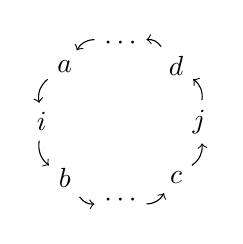
\begin{tikzpicture}
      \begin{scope}[shift={(0,0)}]
\node (0) at ({90 + (360/8 * 0)}:1) {\( \cdots \)};
\node (1) at ({90 + (360/8 * 1)}:1) {\( a \)};
\node (2) at ({90 + (360/8 * 2)}:1) {\( i \)};
\node (3) at ({90 + (360/8 * 3)}:1) {\( b \)};
\node (4) at ({90 + (360/8 * 4)}:1) {\( \cdots \)};
\node (5) at ({90 + (360/8 * 5)}:1) {\( c \)};
\node (6) at ({90 + (360/8 * 6)}:1) {\( j \)};
\node (7) at ({90 + (360/8 * 7)}:1) {\( d \)};
\draw[->,bend right] (0) to (1);
\draw[->,bend right] (1) to (2);
\draw[->,bend right] (2) to (3);
\draw[->,bend right] (3) to (4);
\draw[->,bend right] (4) to (5);
\draw[->,bend right] (5) to (6);
\draw[->,bend right] (6) to (7);
\draw[->,bend right] (7) to (0);
\end{scope}
    \end{tikzpicture} \qquad \qquad \qquad 
    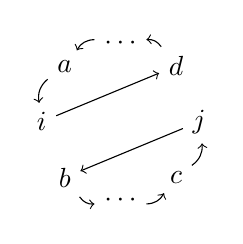
\begin{tikzpicture}
      \begin{scope}[shift={(0,0)}]
\node (0) at ({90 + (360/8 * 0)}:1) {\( \cdots \)};
\node (1) at ({90 + (360/8 * 1)}:1) {\( a \)};
\node (2) at ({90 + (360/8 * 2)}:1) {\( i \)};
\node (3) at ({90 + (360/8 * 3)}:1) {\( b \)};
\node (4) at ({90 + (360/8 * 4)}:1) {\( \cdots \)};
\node (5) at ({90 + (360/8 * 5)}:1) {\( c \)};
\node (6) at ({90 + (360/8 * 6)}:1) {\( j \)};
\node (7) at ({90 + (360/8 * 7)}:1) {\( d \)};
\draw[->,bend right] (0) to (1);
\draw[->,bend right] (1) to (2);
\draw[->] (2) to (7);
\draw[->,bend right] (3) to (4);
\draw[->,bend right] (4) to (5);
\draw[->,bend right] (5) to (6);
\draw[->] (6) to (3);
\draw[->,bend right] (7) to (0);
\end{scope}
    \end{tikzpicture}
    \caption{A cycle \( \rho \) with \( i \) and \( j \) on the left
      and the permutation \( \rho\tau \) on the right, where
      \( \tau=(i,j) \).}
    \label{fig:mult-tau}
  \end{figure}
\end{proof}


\begin{lem}\label{lem:inv+1}
  Let \( \pi\in \sym_n \) and let \( \tau=(i,i+1)\in\sym_n \). Then
  \[
    \sgn(\pi\tau) =  - \sgn(\pi).
  \]
\end{lem}

\begin{proof}
  Since
  \[
    \pi\tau =
    \begin{pmatrix}
      \cdots & i & i+1 & \cdots \\
      \cdots & \pi_{i+1} & \pi_i & \cdots 
    \end{pmatrix},
  \]
  we have \( \inv(\pi\tau) = \inv(\pi)\pm 1 \). This implies
  \( \sgn(\pi\tau) = - \sgn(\pi) \).
\end{proof}


\begin{lem}\label{lem:sgn=trans}
  If \( \pi\in \sym_n \) is a product of \( k \) simple transpositions, then
  \[
    \sgn(\pi) = (-1)^k.
  \]
\end{lem}
\begin{proof}
  Let \( \pi = t_1 \cdots t_k \), where \( t_i \)'s are simple
  transpositions. Then by \Cref{lem:sgn=trans},
  \[
    \sgn(\pi) = \sgn(\iota t_1 \cdots t_k) = (-1)^{k}\sgn(\iota) = (-1)^{k}.
  \]
\end{proof}

\begin{prop}
    For two permutations \( \pi,\sigma\in \sym_n \), we have
  \[
    \sgn(\pi\sigma) = \sgn(\pi) \sgn(\sigma).
  \]
\end{prop}
\begin{proof}
  Suppose \( \pi = t_1 \cdots t_k \) and
  \( \sigma = s_1 \cdots s_r \), where \( t_i \)'s and \( s_r \)'s are
  simple transpositions. Then since \( \sgn(\pi) = (-1)^{k} \)
  \( \sgn(\sigma) = (-1)^{r} \), we have
  \[
    \sgn(\pi\sigma) = \sgn(t_1 \cdots t_k s_1 \cdots s_r) = (-1)^{k+r}
    = \sgn(\pi) \sgn(\sigma). \qedhere
  \]
\end{proof}


\begin{prop}
  For \( \pi\in \sym_n \), we have
  \[
    \sgn(\pi) = (-1)^{\inv(\pi)} = (-1)^{n-\cycle(\pi)} =
    (-1)^{\evencycle(\pi)},
  \]
  where \( \evencycle(\pi) \) is the number of even cycles in
  \( \pi \). In particular, if \( \pi = t_1 \cdots t_k \), where
  \( t_i \)'s are transpositions, then \( \sgn(\pi) = (-1)^{t} \).
\end{prop}
\begin{proof}
  Let \( \pi = t_1 \cdots t_k \), where \( t_i \)'s are simple
  transpositions. By the definition of \( \sgn(\pi) \) and
  \Cref{lem:sgn=trans}, we have
  \( \sgn(\pi) = (-1)^{\inv(\pi)} = (-1)^{k} \). On the other hand,
  since \( \pi = t_1 \cdots t_k\iota \), by \Cref{lem:cycle+1},
  \( (-1)^{\cycle(\pi)} = (-1)^{\cycle(\iota)+k} = (-1)^{n+k} \).
  Thus \( \sgn(\pi) = (-1)^{k} = (-1)^{n-\cycle(\pi)} \).

  Now let \( c_i \) be the number of cycles of length \( i \) in
  \( \pi \). Then
  \[
    (-1)^{n-\cycle(\pi)} = (-1)^{(1\cdot c_1 + 2\cdot c_2 + \cdots + n
      \cdot c_n) - (c_1 + \cdots + c_n)} =(-1)^{0\cdot c_1 + 1\cdot
      c_2 + \cdots + (n-1) \cdot c_n} = (-1)^{n-\cycle(\pi)}.
  \]

  The last statement follows from
  \[
    \sgn(\pi) = \sgn(t_1 \cdots t_k) = \sgn(t_1) \cdots \sgn(t_k)
    = (-1)^{k},
  \]
  because the sign of a transposition \( \tau \) is
  \( \sgn(\tau) = (-1)^{\evencycle(\tau)} = (-1)^1 = -1 \).
\end{proof}

The \emph{signless Stirling number of the first kind} \( c(n,k) \) is
defined to be the number of permutations on \( [n] \) with \( k \)
cycles. The \emph{Stirling number of the first kind} \( s(n,k) \) is
defined to by \( s(n,k) = (-1)^{n-k} c(n,k) \). Note that
\( (-1)^{n-k} \) is the sign of a permutation on \( [n] \) with
\( k \) cycles.

\begin{prop}
  For integers \( n,k\ge1 \), we have
  \begin{equation}\label{eq:c(n,k)-rec}
    c(n,k) = c(n-1,k-1) + (n-1) c(n-1,k).
  \end{equation}
\end{prop}
\begin{proof}
  A permutation \( \pi \in \sym_n \) can be obtained from a
  permutation \( \pi'\in \sym_{n-1} \) by creating a new cycle
  \( (n) \) of length \( 1 \) or by inserting \( n \) after any
  integer in a cycle of \( \pi' \). For example, for
  \( \pi' = (1,9,3)(2,5)(4,8) (6) (7) \in \sym_9 \), if we insert
  \( 10 \) after \( 2 \), we get
  \( \pi = (1,9,3)(2,10,5)(4,8) (6) (7) \in \sym_{10} \), if we insert
  \( 10 \) after \( 6 \), we get
  \( \pi = (1,9,3)(2,5)(4,8) (6,10) (7) \in \sym_{10} \), and if we
  create a new cycle with \( 10 \), we get
  \( \pi = (1,9,3)(2,5)(4,8) (6) (7) (10) \in \sym_{10} \). This shows
  the recursion.
\end{proof}


\begin{prop}
  We have
  \begin{equation}\label{eq:s(n,k)}
    \sum_{k=0}^{n} s(n,k) x^k = (x)_n.
  \end{equation}
  Equivalently,
  \begin{equation}\label{eq:c(n,k)}
    \sum_{k=0}^{n} c(n,k) x^k = x(x+1) \cdots (x+n-1).
  \end{equation}
\end{prop}

\begin{proof}
  The equivalence of \eqref{eq:s(n,k)} and \eqref{eq:c(n,k)} is
  obtained by replacing \( x \) by \( -x \) and multiplying
  \( (-1)^{n} \) both sides.
  Thus it suffices to show \eqref{eq:c(n,k)}.
  This can be proved by induction using \eqref{eq:c(n,k)-rec}.
\end{proof}

Note that \eqref{eq:c(n,k)} can be rewritten as
\begin{equation}\label{eq:c(n,k)-gf}
   \sum_{\pi\in \sym_n}  x^{\cycle(\pi)} = x(x+1) \cdots (x+n-1).
\end{equation}
We can prove this bijectively.

\begin{proof}[A bijective proof of \eqref{eq:c(n,k)-gf}]
  We will construct an algorithm to construct a permutation
  \( \pi\in \sym_n \).
  For \( k=1,\dots,n \), we do the following.
  \begin{description}
  \item[Step 1] For \( k=1 \), create a new cycle consisting of \( 1 \).
  \item[Step 2] Let \( 2\le k\le n \) and suppose that the integers
    \( 1,\dots,k-1 \) form a permutation on \( [k-1] \) in cycle
    notation. Then we either create a new cycle consisting of \( k \)
    or insert \( k \) after one of the integers \( 1,\dots,k-1 \).
  \end{description}

  For each \( 1\le k\le n \), there are \( k \) choices: creating a
  new cycle (in one way) or inserting \( k \) into one of the existing
  cycles (in \( k-1 \) ways). The possible choices for \( k \) are
  exactly the same as the choices for the \( k \)th factor when we
  expand
  \begin{equation}\label{eq:19}
    x(x+1)(x+1+1)\cdots (x+\overbrace{1+1 + \cdots + 1}^{n-1}).
  \end{equation}
  Moreover, the first choice (creating a new cycle) corresponds to
  multipying \( x \). Thus, if \( \pi \) is a permutation obtained in
  this algoritm, then the same process in the exansion of
  \eqref{eq:19} gives \( x^{\cycle(\pi)} \). This means that the both
  sides of\eqref{eq:c(n,k)-gf} match term-by-term, completing the
  proof of this identity.
\end{proof}


Using \eqref{eq:S(n,k)(x)k=xn} and \eqref{eq:s(n,k)} we obtain the
following matrix identity, which is a duality between Stirling numbers
of the first and second kinds.


\begin{prop}
  We have
 \begin{equation}\label{eq:18}
   \Big(S(n,k)\Big)_{n,k\ge0} \Big(s(n,k)\Big)_{n,k\ge0} = I,
 \end{equation} 
 where \( I= (\delta_{n,k})_{n,k\ge0} \) is the infinite identity
 matrix.
 Equivalently, for integers \( n,m\ge0 \),
 \begin{align}
   \label{eq:S-s-dual}
   \sum_{k\ge0} S(n,k)s(k,m) & = \delta_{n,m},\\
   \label{eq:s-S-dual}
   \sum_{k\ge0} s(n,k)S(k,m) & = \delta_{n,m}.
 \end{align}
\end{prop}

\begin{proof}
  By \eqref{eq:S(n,k)(x)k=xn} and \eqref{eq:s(n,k)}, we have
  the change of basis identities between
  two bases \( \{x^n\}_{n\ge0} \) and \( \{(x)_n\}_{n\ge0} \)
  of the vector space of polynomials:
  \begin{align*}
   \Big(S(n,k)\Big)_{n,k\ge0} \Big((x)_n\Big)_{n\ge0} &=  \Big(x^n\Big)_{n\ge0},\\
   \Big(s(n,k)\Big)_{n,k\ge0} \Big(x^n\Big)_{n\ge0} &=  \Big((x)_n\Big)_{n\ge0}.
 \end{align*}
 Thus the two matrices \( (S(n,k))_{n,k\ge0} \) and
 \( (s(n,k))_{n,k\ge0} \) are inverse of each other, proving
 \eqref{eq:18}.
\end{proof}


\chapter{Combinatorial models for OPS}
\label{sec:comb-interpr-orth}

From now one we will focus on the combinatorial approaches to
orthogonal polynomials in Viennot's lecture notes \cite{ViennotLN}.
A part of this chapter has some overlaps with \Cref{sec:basics-orth-polyn}.

The main goal of this chapter to give combinatorial interpretations
for orthogonal polynomials and their moments. Using these
combinatorial interpretations, we will reprove the orthogonality of
orthogonal polynomials using combinatorics only.

\section{Orthogonal polynomials and 3-term recurrences}

In this section we recall basic definitions and properties of
orthogonal polynomials. We then state the 3-term recurrence of
orthogonal polynomials and Favard's theorem.

Let \( K \) be a field (we can also use a commutative ring for any
result without using divisions). We denote by \( K[x] \) the ring of
polynomials in \( x \) with coefficients in \( K \). A \emph{linear
  functional} is a linear transformation \( \LL:K[x]\to K \), i.e., a
function satisfying \( \LL(af(x)+bg(x)) = a \LL(f(x))+b \LL(g(x)) \)
for all \( f(x),g(x)\in K[x] \) and \( a,b\in K \). The \( n \)th
\emph{moment} of \( \LL \) is defined to be \( \mu_n = \LL(x^n) \).

\begin{defn}\label{def:formal-ops}
  Let \( \LL \) be a linear functional defined on the space of
  polynomials in \( x \). A sequence of polynomials
  \( \{P_n(x)\}_{n\ge0} \) is called an \emph{orthogonal polynomial
    sequence (OPS)} with respect to \( \LL \) if the following
  conditions hold:
  \begin{enumerate}
  \item \( \deg P_n(x) = n \), \( n\ge0 \),
  \item \( \LL(P_m(x)P_n(x))  = 0 \) for \( m\ne n \),
  \item \( \LL(P_m(x)^2) \ne 0 \) for \( m\ge0 \).
  \end{enumerate}
  We also say that \( \{ P_n(x) \}_{n\ge 0} \) is orthogonal
  for the moments \( \{\mu_n\}_{n\ge0} \).
\end{defn}

Orthogonal polynomials in the above definition are called ``formal''
or ``general'' orthogonal polynomials because the field \( K \) can be
anything. For instance, it may contain arbitrary formal variables such
as \( a,b,c,d \). Then the polynomials \( P_n(x) \) and the moments
\( \mu_n \) can be treated as polynomials (or more complicated objects
such as formal power series or rational functions) in these formal
variables.

\begin{prop}
  Suppose that \( \{ P_n(x) \}_{n\ge 0} \) is an OPS for \( \LL \).
\begin{enumerate}
\item \( \{ P_n(x) \}_{n\ge 0} \) is also orthogonal with respect to
  \( \LL' \) for any \( \LL' = a\LL \) for \( a\ne 0 \).
\item \( \LL \) is uniquely determined up to
  nonzero scalar multiplication. 
\item If we set \( \LL(1) = 1 \), then \( \LL \) is uniquely
  determined.
\item \( \{ a_nP_n(x) \}_{n\ge 0} \) is an OPS with respect to
  \( \LL \) for any sequence \( \{ a_n\}_{n\ge 0} \) with
  \( a_n\ne 0 \).
\end{enumerate}
\end{prop}

\begin{proof}
  All statements are easy to check. For example, (2) can be seen by
  noticing that once the \( 0 \)th moment \( \mu_0=\LL(1) \) is
  determined, then the \( n \)th moment \( \mu_n \), for \( n\ge1 \),
  is uniquely determined by the condition \( \LL(P_n(x)) = 0 \).
\end{proof}

By the above proposition we may assume that \( \LL(1) = 1 \).
\emph{From now on we will always assume that \( \deg P_n(x) = n \) and
  \( \LL(1) = 1 \) unless otherwise stated.}

Recall from \Cref{thm:3-RR} that every OPS satisfies a 3-term
recurrence.

\begin{thm}[3-term recurrence]
  Let \( \LL \) be a linear functional with monic OPS
  \( \{ P_n(x) \}_{n\ge 0} \). Then there are sequences
  \( \{ b_n\}_{n\ge 0} \) and \( \{ \lambda_n\}_{n\ge 1} \) such that
  \( \lambda_n\ne 0 \) and
  \[
    P_{n+1}(x) = (x-b_n) P_n(x) - \lambda_n P_{n-1}(x), \qquad n\ge0,
  \]
  where \( P_{-1}(x) = 0 \) and \( P_0(x) = 1 \).
\end{thm}

The inverse of the above theorem is also true, which is one of the
most important results in the theory of classical orthogonal
polynomials.

\begin{thm}[Favard's theorem]
  Let \( \{ P_n(x) \}_{n\ge 0} \) be a sequence of polynomials
  satisfying \( P_{-1}(x) = 0 \), \( P_0(x) = 1 \), and
  \begin{equation}\label{eq:3-RR}
    P_{n+1}(x) = (x-b_n) P_n(x) - \lambda_n P_{n-1}(x), \qquad n\ge0,
  \end{equation}
  for some sequences \( \{ b_n\}_{n\ge 0} \) and
  \( \{ \lambda_n\}_{n\ge 1} \) with \( \lambda_n\ne 0 \). 
 Then
  \( \{ P_n(x) \}_{n\ge 0} \) is an OPS for some linear functional
  \( \LL \).
\end{thm}

The main goal of this chapter is to give combinatorial interpretations
for the orthogonal polynomials \( P_n(x) \) and their moments
\( \mu_n \). Using these combinatorial interpretations we will prove
Favard's theorem bijectively.

\section{A model for orthogonal polynomials using Favard tilings}

In this section we give a combinatorial interpretation for
orthogonal polynomials using Favard tilings.


\begin{defn}
  A \emph{Favard tiling of size $n$} is a tiling of a $1\times n$
  square board with three types of tiles: red monominos, black
  monominos, and black dominos. The set of Favard tilings of size $n$
  is denoted by $\FT_n$.

  We label the squares in the $1\times n$ board by $0,1,\dots,n-1$
  from left to right. Define the weight \( \wt(T) \) of
  \( T\in \FT_n \) to be the product of the weights of the tiles in
  \( T \), where
  \begin{enumerate}
  \item the weight of each red monomino is \( x \),
  \item the weight of each black monomino containing a label
    \( i \) is \( -b_i \), and
  \item the weight of each domino containing labels \( i-1 \) and
    \( i \) is \( -\lambda_i \).
  \end{enumerate}




\end{defn}

For example, see \Cref{fig:tiling}. Note that the number \( u_n \) of
Favard tilings of size \( n \) satisfies \( u_{n+1} = 2u_n+u_{n-1} \)
with \( u_0=1 \) and \( u_1=2 \). These numbers are called the Pell
numbers.

\begin{figure}
  \centering
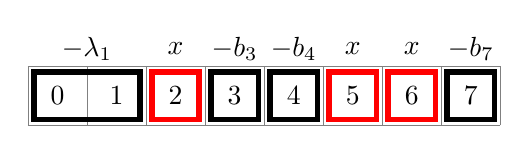
\begin{tikzpicture}[scale=0.75]
  \draw [help lines] (0,0) grid (8,1);
  \foreach \x in {0,...,7} \draw node at (\x+.5,.5) {\x};
  \LBD1 \LRM2 \LBM3 \LBM4 \LRM5 \LRM6 \LBM7
\end{tikzpicture}
\caption{A Favard tiling $T\in\FT_8$ with
  $\wt(T)=\lambda_1 b_3b_4b_7x^3$.}
  \label{fig:tiling}
\end{figure}

The following proposition gives a combinatorial interpretation for
orthogonal polynomials.

\begin{prop}\label{pro:Favard}
  Suppose that \( \{ P_n(x) \}_{n\ge 0} \) is a sequence of
  polynomials satisfying \eqref{eq:3-RR}. Then
  \[
    P_n(x) = \sum_{T\in \FT_n} \wt(T).
  \]
\end{prop}
\begin{proof}
  This is immediate from the recurrence \eqref{eq:3-RR}.
\end{proof}


\section{How to find a combinatorial model for moments}

Moments are important quantities of a linear functional \( \LL \)
because they have all the information of \( \LL \). In this section
we will find a combinatorial interpretation for the moments of
orthogonal polynomials. To do this we will first take a close look at
the moments.

Suppose that \( \LL \) is a linear functional with monic OPS
\( \{ P_n(x) \}_{n\ge 0} \), which satisfies the 3-term recurrence
\eqref{eq:3-RR}. Let's assume \( \LL(1)=1 \). Then, using the
orthogonality, we have
\begin{equation}\label{eq:13}
  \LL(P_n(x)) = \delta_{n,0}.
\end{equation}
This relation in fact completely determines the moments \( \mu_n \).
For example, since
\begin{align*}
  P_0(x) &= 1,\\
  P_1(x) &= (x-b_0)P_0(x) - \lambda_0P_{-1}(x) = x-b_0,\\
  P_2(x) &= (x-b_1)P_1(x) - \lambda_1P_0(x) =  x^2 - (b_1+b_0)x +b_0b_1 - \lambda_1,
\end{align*}
we have
\begin{align*}
 \mu_0 &= \LL(1) = 1, \\
 \mu_1 &= \LL(x) = \LL(P_1(x)+b_0) = b_0, \\
  \mu_2 &= \LL(x^2) = \LL(P_2(x)+(b_0+b_1)x-b_0b_1+\lambda_1)
          = (b_0+b_1)b_0 - b_0b_1 +\lambda_1 = b_0^2+\lambda_1.
\end{align*}
In this way, we can compute a few more moments:
\begin{align*}
  \mu_3 &= b_0^3 + 2b_0\lambda_1 + b_1\lambda_1,\\
  \mu_4 &= b_0^4 + 3b_0^2\lambda_1 + 2b_0b_1\lambda_1 + b_1^2\lambda_1 + \lambda_1^2 + \lambda_1\lambda_2,\\
  \mu_5 &= b_0^5 + 4b_0^3\lambda_1 + 3b_0^2b_1\lambda_1 + 2b_0b_1^2\lambda_1 + b_1^3\lambda_1 + 3b_0\lambda_1^2 + 2b_1\lambda_1^2 + 2b_0\lambda_1\lambda_2 + 2b_1\lambda_1\lambda_2 + b_2\lambda_1\lambda_2.
\end{align*}

The above experiments clearly suggest that \( \mu_n \) would be a
polynomial in \( b_i \)'s and \( \lambda_i \)'s with nonnegative
integer coefficients. How can we prove such a conjecture? A satisfying
answer to this question is to find combinatorial objects whose
generating function is \( \mu_n \). That is to find a set \( X \) of
combinatorial objects and a weight \( \wt(A) \) of each element
\( A\in X \) such that
\[
  \mu_n = \sum_{A \in X} \wt(A),
\]
and \( \wt(A) \) is a polynomial (preferably a monomial) in
\( b_i \)'s and \( \lambda_i \)'s with nonnegative integer
coefficients.

But how can we find such combinatorial objects? Suppose that such
combinatorial objects exist with monomial weight \( \wt(A) \) for each
\( A\in X \). Then if we set \( b_i=\lambda_i=1 \) for all \( i \)
then \( \mu_n \) would be the number of elements in \( X \). If we
compute \( \mu_n \) with this substitution for \( n=0,1,2,\ldots \),
then we obtain the following sequence:
\[
  1, 1, 2, 4, 9, 21, 51, 127, 323, 835, 2188, 5798, 15511, \ldots.
\]
There is a very useful webpage \url{https://oeis.org/} where you can
search integer sequences. If you search the above sequence, the
webpage will tell you that this is the sequence of the number of
Motzkin paths. So we can guess that there must be a close connection
with the moments of orthogonal polynomials and Motzkin paths.

After spending enough time of trials and errors, we can come up with
the following combinatorial model for the moments of orthogonal
polynomials.

Recall that \( \Motz(u\to v) \) is the set of Motzkin paths from
\( u \) to \( v \). We define the weight \( \wt(\pi) \) of a Motzkin
path \( \pi \) to be the product of the weights of the steps in
\( \pi \), where
\begin{enumerate}
\item the weight of an up step is \( 1 \),
\item the weight of a horizontal step starting at height \( i \) is \( b_i \), and
\item the weight of a down step starting at height \( i \) is
  \( \lambda_i \).
\end{enumerate}
See \Cref{fig:Motzkin-wt}.

\begin{figure}
  \centering
  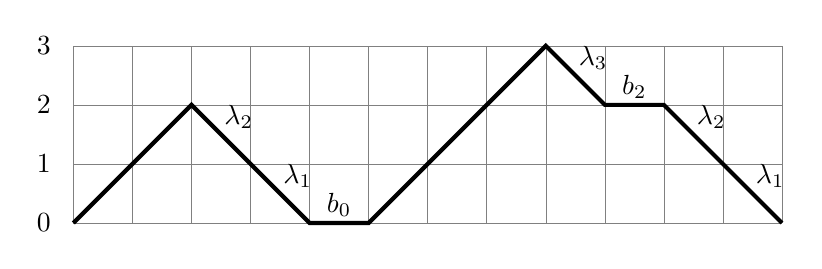
\begin{tikzpicture}[scale=0.75]
    \draw[help lines] (0,0) grid (12,3);
    \foreach \y in {0,...,3} \draw node at (-.5,\y) {$\y$};
\draw[line width = 1.5pt] (0,0) -- ++(1,1) -- ++(1,1) -- ++(1,-1) -- ++(1,-1) -- ++(1,0) -- ++(1,1) -- ++(1,1) -- ++(1,1) -- ++(1,-1) -- ++(1,0) -- ++(1,-1) -- ++(1,-1);
    \node at (2.8,1.8) {$\lambda_{2}$};
    \node at (3.8,0.8) {$\lambda_{1}$};
    \node at (4.5,0.3) {$b_{0}$};
    \node at (8.8,2.8) {$\lambda_{3}$};
    \node at (9.5,2.3) {$b_{2}$};
    \node at (10.8,1.8) {$\lambda_{2}$};
    \node at (11.8,0.8) {$\lambda_{1}$};
\end{tikzpicture}
\caption{A Motzkin path $\pi$ from $(0,0)$ to $(12,0)$ with
  $\wt(\pi)=b_0b_2\lambda_1^2\lambda_2^2\lambda_3$.}
  \label{fig:Motzkin-wt}
\end{figure}

We are now ready state Viennot's combinatorial interpretation for
moments of orthogonal polynomials.

\begin{thm}\label{thm:mu=Mot}
  Suppose that \( \{ P_n(x) \}_{n\ge 0} \) is a monic OPS for a
  linear functional \( \LL \) with \( \LL(1)=1 \). Suppose that
  \( \{ P_n(x) \}_{n\ge 0} \) satisfy the 3-term recurrence
  \[
      P_{n+1}(x) = (x-b_n) P_n(x) - \lambda_n P_{n-1}(x), \qquad n\ge0.
  \]
  Then the moments \( \mu_n=\LL(x^n) \) are given by
\[
  \mu_n = \sum_{\pi\in \Motz_n} \wt(\pi).
\]
\end{thm}

More generally, we will prove
a combinatorial interpretation for mixed moments.

\begin{defn}\label{def:mixed_moment}
  Let \( \{ P_n(x) \}_{n\ge 0} \) be a monic OPS for a linear
  functional \( \LL \). For integers \( n,r,s\ge0 \), the \emph{mixed
    moments} \( \mu_{n,r,s} \) and \( \mu_{n,k} \) of this OPS are
  defined by
  \begin{align*}
    \mu_{n,r,s} &= \frac{\LL(x^n P_r(x)P_s(x))}{\LL(P_s(x)^2)},\\
    \mu_{n,k} &= \mu_{n,0,k} = \frac{\LL(x^n P_k(x))}{\LL(P_k(x)^2)}.
  \end{align*}
\end{defn}

Note that \( \mu_n = \mu_{n,0,0} \).

Let \( \Motz_{n,r,s} \) denote the set of Motzkin paths from
\( (0,r) \) to \( (n,s) \). 

\begin{thm}\label{thm:mu=Mot_nrs}
  Following the notation in \Cref{thm:mu=Mot}, we have
\[
  \mu_{n,r,s} = \sum_{\pi\in \Motz_{n,r,s}} \wt(\pi).
\]
\end{thm}

\begin{proof}
  We proceed by induction on \( n \).
  Suppose \( n=0 \). By the orthogonality of \( \{ P_n(x) \}_{n\ge 0} \),
  we have
  \[
    \mu_{0,r,s} = \frac{\LL(P_r(x)P_s(x))}{\LL(P_s(x)^2)} = \delta_{r,s}.
  \]
  Since \( \Motz_{0,r,s} = \emptyset \) if \( r=s \) and
  \( \Motz_{0,r,s} \) has only one (empty) Motzkin path if \( r=s \),
  we also have
  \( \sum_{\pi\in \Motz_{n,r,s}} \wt(\pi) = \delta_{r,s} \).

  Let \( n\ge1 \) and suppose that the theorem holds for \( n-1 \).
  Then by the 3-term recurrence,
  \[
    xP_r(x) = P_{r+1}(x) + b_rP_r(x) + \lambda_rP_{r-1}(x).
  \]
  Thus
  \begin{align*}
    \mu_{n,r,s}
    &= \frac{\LL(x^n P_r(x) P_s(x))}{\LL(P_s(x)^2)}
      = \frac{\LL(x^{n-1} (xP_r(x)) P_s(x))}{\LL(P_s(x)^2)}\\
    &=\frac{\LL(x^{n-1} (P_{r+1}(x) + b_rP_r(x) + \lambda_rP_{r-1}(x)) P_s(x))}{\LL(P_s(x)^2)} \\
    &= \frac{\LL(x^{n-1} P_{r+1}(x)P_s(x))}{\LL(P_s(x)^2)}
      + b_r\frac{\LL(x^{n-1} P_r(x)P_s(x))}{\LL(P_s(x)^2)}
      + \lambda_r \frac{\LL(x^{n-1} P_{r-1}(x)P_s(x))}{\LL(P_s(x)^2)}\\
    &= \mu_{n-1,r+1,s} + b_r\mu_{n-1,r,s} + \lambda_r \mu_{n-1,r-1,s}\\
    &= \sum_{\pi\in \Motz_{n-1,r+1,s}} \wt(\pi)
    + b_r \sum_{\pi\in \Motz_{n-1,r,s}} \wt(\pi)
    + \lambda_r \sum_{\pi\in \Motz_{n-1,r-1,s}} \wt(\pi)\\
      &=      \sum_{\pi\in \Motz_{n,r,s}} \wt(\pi),
  \end{align*}
  where the second to last equation follows from the induction
  hypothesis and the last equation follows from considering the first
  step of each \( \pi\in \Motz_{n,r,s} \). Hence the theorem holds for
  \( n \) and we are done by induction.
\end{proof}

\begin{cor}
  Following the notation in \Cref{thm:mu=Mot}, we have
  \[
    \LL(P_n(x)^2) = \lambda_1 \cdots \lambda_n.
  \]
\end{cor}

\begin{proof}
  Since \( P_n(x) \) is monic, we can write \( P_n(x) = x^n + Q(x) \)
  for some polynomial \( Q(x) \) of degree less than \( n \). Thus
  by \Cref{thm:mu=Mot_nrs},
  \[
    \LL(P_n(x)^2) = \LL((x^n + Q(x))P_n(x)) = \LL(x^n P_n(x))
    = \sum_{\pi\in \Motz_{n,n,0}} \wt(\pi) = \lambda_1 \cdots \lambda_n,
  \]
  as desired. Here, the last equality follows from the fact that there
  is only one Motzkin path in \( \Motz_{n,n,0} \), namely, the path
  from \( (0,n) \) to \( (n,0) \) consisting of \( n \) down steps.
\end{proof}

\section{A bijective proof of Favard's theorem}

We have a combinatorial interpretation for both orthogonal polynomials
and their moments. In this section we will prove Favard's theorem
bijectively using these combinatorial models.


Suppose that \( \{ P_n(x) \}_{n\ge 0} \) is a sequence of polynomials
satisfying the 3-term recurrence
\[
  P_{n+1}(x) = (x-b_n) P_n(x) - \lambda_n P_{n-1}(x).
\]
To prove Favard's theorem, we need to find a linear functional
\( \LL \) for which \( \{ P_n(x) \}_{n\ge 0} \) are orthogonal.
We simply define \( \LL \) so that the moments are given by
\begin{equation}\label{eq:8}
  \LL(x^n) = \sum_{\pi\in \Motz_{n}} \wt(\pi).
\end{equation}
It is enough to show that
\[
  \LL(P_r(x)P_s(x)) = \lambda_1 \cdots \lambda_s \delta_{r,s}.
\]
More generally, we will prove
\begin{equation}\label{eq:LL(xPP)}
  \LL(x^n P_r(x)P_s(x)) = \lambda_1 \cdots \lambda_s \sum_{\pi\in
    \Motz_{n,r,s}} \wt(\pi).
\end{equation}

We first need to give a combinatorial meaning to the the left-hand
side of \eqref{eq:LL(xPP)}. For a Favard tiling \( T \) with \( k \)
red monominos, let \( \wt'(T) = \wt(T)/x^k \). In other words,
\( \wt'(T) \) is the same as \( \wt(T) \) except we only consider the
weights of black monominos and black dominos.
Then \Cref{pro:Favard} can be restated as
\[
  P_n(x) = \sum_{T\in \FT_n} \wt'(T) \cdot x^{(\text{number of red monominos in \( T \)})}.
\]
Thus, by the definition of \( \LL(x^n) \) in \eqref{eq:8}, we have
\[
    \LL(x^n P_r(x)P_s(x)) = 
    \sum_{(T_1,T_2,\pi)\in X} \wt'(T_1) \wt'(T_2) \wt(\pi),
\]
where \( X \) is the set of triples \( (T_1,T_2,\pi) \)
such that for some \( 0\le i\le r \) and \( 0\le j\le s \),
\begin{enumerate}
\item \( T_1\in \FT_r \) has \( i \) red monominos,
\item \( T_2\in \FT_s \) has \( j \) red monominos, and
\item \( \pi\in \Motz_{n+i+j} \).
\end{enumerate}

Let \( Y \) be the set of \( \pi\in \Motz_{n+r+s} \) such that the
first \( r \) steps are up steps and the last \( s \) step s are down
steps. Then the right-hand side of \eqref{eq:LL(xPP)} is equal to
\( \sum_{\pi\in Y} \wt(\pi) \). Therefore \eqref{eq:LL(xPP)} is
equivalent to the following theorem.

\begin{thm}\label{thm:5}
  For the sets \( X \) and \( Y \) defined above, we have
\begin{equation}\label{eq:LL(xPP)2}
  \sum_{(T_1,T_2,\pi)\in X} \wt'(T_1) \wt'(T_2) \wt(\pi)
  =  \sum_{\pi\in Y} \wt(\pi).
\end{equation}
\end{thm}

\begin{proof}
  We will find a sign-reversing weight-preserving involution on
  \( X \) with fixed point set
  \( \{ (\emptyset,\emptyset,\pi):\pi\in Y\} \). Consider
  \( (T_1,T_2,\pi)\in X \). We write \( \pi=S_1S_2 \cdots S_{m} \) as
  a sequence of steps. Let \( a,b,u,v \) be the integers defined as follows:
 \begin{itemize}
 \item \( a \) is the largest integer such that \( T_1 \)
   starts with \( a \) red monominos,
 \item \( b \) is the largest integer such that \( T_2 \)
   starts with \( b \) red monominos,
 \item \( u \) is the largest integer such that \( \pi \) starts with
   \( u \) up steps,
 \item \( v \) is the largest integer such that \( \pi \) ends with
   \( v \) down steps.
 \end{itemize}

 We now define \( \phi(T_1,T_2,\pi)= (T'_1,T'_2,\pi') \) in the following
 way. Here, \( a',b',u',v' \) are the integers defined similarly as
 above using \( T'_1 \), \( T'_2 \), and \( \pi' \).
\begin{description}
\item[Case 1] \( u<a \). In this case we set \( T'_2 = T_2 \). There are two
  subcases.
\begin{description}
\item[Case 1-1] \( S_{u+1} \) is a horizontal step. Let
    \[
      \pi' = S_1\cdots \widehat{S_{u+1}} \cdots S_{m},
\]
and define $T_1'$ to be the Favard tiling obtained from $T_1$ by
replacing the \( (u+1) \)st red monomino (at position \( u \)) by a
black monomino. Here the notation $\widehat{S_{u+1}}$ means that
$S_{u+1}$ is removed from the sequence. See Figure~\ref{fig:case-1}.
Observe that since \( \wt'(T'_1) = -b_u \wt'(T_1) \) and
\( \wt'(\pi') = \wt'(\pi)/ b_u \), we have
\[ \wt'(T'_1)\wt'(T'_2)\wt(\pi') = - \wt'(T_1)\wt'(T_2)\wt(\pi). \]
Moreover, we always have \( u'\ge u \) and \( a'=u<a\le r \), hence
\( u'\ge a'\ne r \).
\item[Case 1-2] $S_{u+1}$ is a down step. Let
    \[
      \pi' = S_1\cdots \widehat{S_{u}}\widehat{S_{u+1}} \cdots S_m,
\]
and define $T_1'$ to be the Favard tiling obtained from $T_1$ by
replacing the \( u \)th and \( (u+1) \)st red monominos (at positions
$u-1$ and $u$) by a domino. See Figure~\ref{fig:case-2}. 
Observe that since \( \wt'(T'_1) = -\lambda_u \wt'(T_1) \) and
\( \wt'(\pi') = \wt'(\pi)/ \lambda_u \), we have
\[ \wt'(T'_1)\wt'(T'_2)\wt(\pi') = - \wt'(T_1)\wt'(T_2)\wt(\pi). \]
Moreover, we always have \( u'\ge u-1 \) and \( a'=u-1<a\le r \),
hence \( u'\ge a'\ne r \).
\end{description}

\item[Case 2] \( u\ge a\ne r \). In this case we set \( T'_2=T_2 \). Let
  \( A \) be the \( (a+1) \)st tile in \( T_1 \) (\( A \) starts at position
  \( a \)). There are two subcases.
  \begin{description}
  \item[Case 2-1] $A$ is a black monomino. In this case let
    \[
      \pi' = S_1\cdots S_a H S_{a+1} \cdots S_m,
\]
and define $T_1'$ to be the Favard tiling obtained from $T_1$ by
replacing $A$ by a red monomino. See Figure~\ref{fig:case-1} (with the
roles of \( (T_1,T_2,\pi) \) and \( (T'_1,T'_2,\pi') \) interchanged).
\item[Case 2-2] $A$ is a domino. In this case let
    \[
      \pi' = S_1\dots S_a UD S_{a+1} \dots S_m,
\]
and define $T_1'$ to be the Favard tiling obtained from $T_1$ by
replacing $A$ by two red monominos. See Figure~\ref{fig:case-2} (with
the roles of \( (T_1,T_2,\pi) \) and \( (T'_1,T'_2,\pi') \)
interchanged).
\end{description}
\item[Case 3] \( u\ge a = r \) and \( v<b \). This can be done
  similarly as Case 1. The only difference is that we set
  \( T_1' = T_1 \) and consider the steps of \( \pi \) from the right.
  
\item[Case 4] \( u\ge a = r \) and \( v\ge b \ne s \).
  This can be done similarly as Case 2.

\item[Case 5] \( u\ge a = r \) and \( v\ge b=s \). In this case we set
  \( (T'_1,T'_2,\pi') = (T_1,T_2,\pi) \). See \Cref{fig:case5}.
\end{description}

\begin{figure}
  \centering
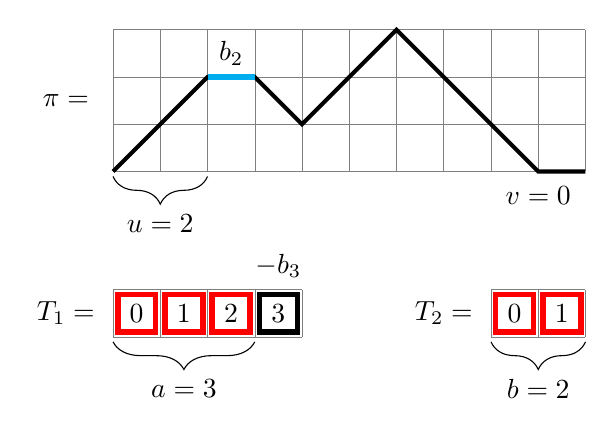
\begin{tikzpicture}[scale=0.6]
  \draw[help lines] (0,0) grid (10,3);
\draw[line width = 1.5pt] (0,0) -- ++(1,1) -- ++(1,1) -- ++(1,0) -- ++(1,-1) -- ++(1,1) -- ++(1,1) -- ++(1,-1) -- ++(1,-1) -- ++(1,-1) -- ++(1,0);
  \draw [decorate,decoration={brace,amplitude=10pt},xshift=-0pt,yshift=-3pt]
(2,0) -- (0,0) node [black,midway,yshift=-0.6cm] {\( u=2 \)};
\node at (-1,1.5) {\( \pi= \)};
\node at (9,-.5) {\( v=0 \)};
\node at (2.5,2.5) {\( b_2 \)};
\draw[line width = 2pt, cyan] (2,2)--++(1,0);
\begin{scope}[shift={(0,-3.5)}]
  \draw [help lines] (0,0) grid (4,1);
  \foreach \x in {0,...,3} \draw node at (\x+0.5,0.5) {\x};
  \RM0 \RM1 \RM2 \BM3
  \node at (3.5,1.5) {\( -b_3 \)};
  \draw [decorate,decoration={brace,amplitude=10pt},xshift=-0pt,yshift=-3pt]
(3,0) -- (0,0) node [black,midway,yshift=-0.6cm] {\( a=3 \)};
\node at (-1,.5) {\( T_1= \)};
\end{scope}
\begin{scope}[shift={(8,-3.5)}]
  \draw [help lines] (0,0) grid (2,1);
  \foreach \x in {0,...,1} \draw node at (\x+0.5,0.5) {\x};
  \RM0 \RM1
  \draw [decorate,decoration={brace,amplitude=10pt},xshift=-0pt,yshift=-3pt]
(2,0) -- (0,0) node [black,midway,yshift=-0.6cm] {\( b=2 \)};
\node at (-1,.5) {\( T_2= \)};
\end{scope}
\end{tikzpicture} \quad
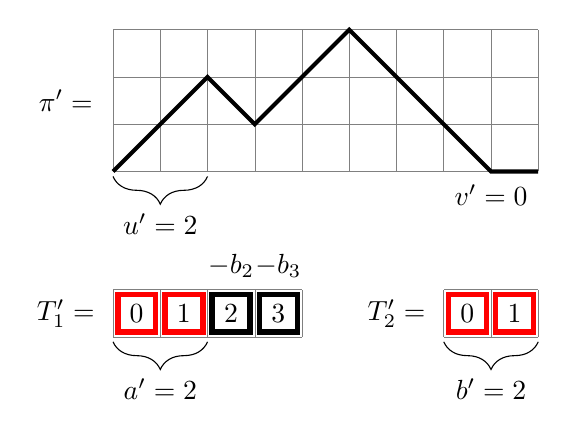
\begin{tikzpicture}[scale=0.6]
  \draw[help lines] (0,0) grid (9,3);
\draw[line width = 1.5pt] (0,0) -- ++(1,1) -- ++(1,1) -- ++(1,-1) -- ++(1,1) -- ++(1,1) -- ++(1,-1) -- ++(1,-1) -- ++(1,-1) -- ++(1,0);
  \draw [decorate,decoration={brace,amplitude=10pt},xshift=-0pt,yshift=-3pt]
(2,0) -- (0,0) node [black,midway,yshift=-0.6cm] {\( u'=2 \)};
\node at (-1,1.5) {\( \pi'= \)};
\remove(2,2)
\node at (8,-.5) {\( v'=0 \)};
\begin{scope}[shift={(0,-3.5)}]
  \draw [help lines] (0,0) grid (4,1);
  \foreach \x in {0,...,3} \draw node at (\x+0.5,0.5) {\x};
  \RM0 \RM1 \BM2 \BM3
  \draw [decorate,decoration={brace,amplitude=10pt},xshift=-0pt,yshift=-3pt]
(2,0) -- (0,0) node [black,midway,yshift=-0.6cm] {\( a'=2 \)};
\node at (-1,.5) {\( T'_1= \)};
  \node at (2.5,1.5) {\( -b_2 \)};
  \node at (3.5,1.5) {\( -b_3 \)};
\end{scope}
\begin{scope}[shift={(7,-3.5)}]
  \draw [help lines] (0,0) grid (2,1);
  \foreach \x in {0,...,1} \draw node at (\x+0.5,0.5) {\x};
  \RM0 \RM1
  \draw [decorate,decoration={brace,amplitude=10pt},xshift=-0pt,yshift=-3pt]
(2,0) -- (0,0) node [black,midway,yshift=-0.6cm] {\( b'=2 \)};
\node at (-1,.5) {\( T'_2= \)};
\end{scope}
\end{tikzpicture}  
\caption{A triple \( (\pi,T_1,T_2)\in X \) in Case 1-1 on the left and
  the corresponding triple \( (\pi',T'_1,T'_2)\in X \) in Case 2-1 on
  the right, where \( r=4 \), \( s=2 \), and \( n=5 \). The horizontal
  step \( (2,2)\to(3,3) \) in \( \pi \) is collapsed to a point.}
  \label{fig:case-1}
\end{figure}

\begin{figure}
  \centering
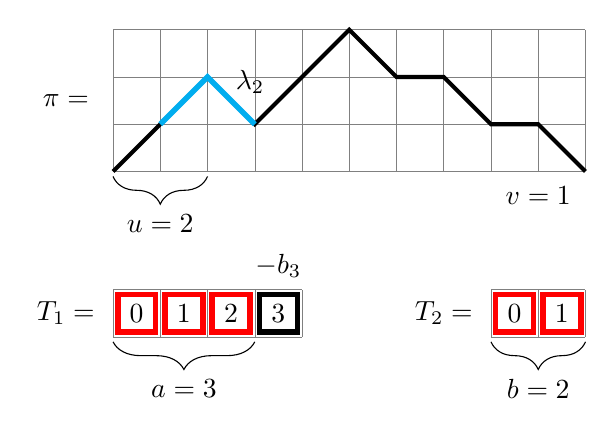
\begin{tikzpicture}[scale=0.6]
  \draw[help lines] (0,0) grid (10,3);
\draw[line width = 1.5pt] (0,0) -- ++(1,1) -- ++(1,1) -- ++(1,-1) -- ++(1,1) -- ++(1,1) -- ++(1,-1) -- ++(1,0) -- ++(1,-1) -- ++(1,0) -- ++(1,-1);
  \draw [decorate,decoration={brace,amplitude=10pt},xshift=-0pt,yshift=-3pt]
(2,0) -- (0,0) node [black,midway,yshift=-0.6cm] {\( u=2 \)};
\node at (-1,1.5) {\( \pi= \)};
\node at (9,-.5) {\( v=1 \)};
\node at (2.9,1.9) {\( \lambda_2 \)};
\draw[line width = 2pt, cyan] (1,1) -- (2,2)--++(1,-1);
\begin{scope}[shift={(0,-3.5)}]
  \draw [help lines] (0,0) grid (4,1);
  \foreach \x in {0,...,3} \draw node at (\x+0.5,0.5) {\x};
  \RM0 \RM1 \RM2 \BM3
  \draw [decorate,decoration={brace,amplitude=10pt},xshift=-0pt,yshift=-3pt]
(3,0) -- (0,0) node [black,midway,yshift=-0.6cm] {\( a=3 \)};
\node at (-1,.5) {\( T_1= \)};
\node at (3.5,1.5) {\( -b_3 \)};
\end{scope}
\begin{scope}[shift={(8,-3.5)}]
  \draw [help lines] (0,0) grid (2,1);
  \foreach \x in {0,...,1} \draw node at (\x+0.5,0.5) {\x};
  \RM0 \RM1
  \draw [decorate,decoration={brace,amplitude=10pt},xshift=-0pt,yshift=-3pt]
(2,0) -- (0,0) node [black,midway,yshift=-0.6cm] {\( b=2 \)};
\node at (-1,.5) {\( T_2= \)};
\end{scope}
\end{tikzpicture} \quad
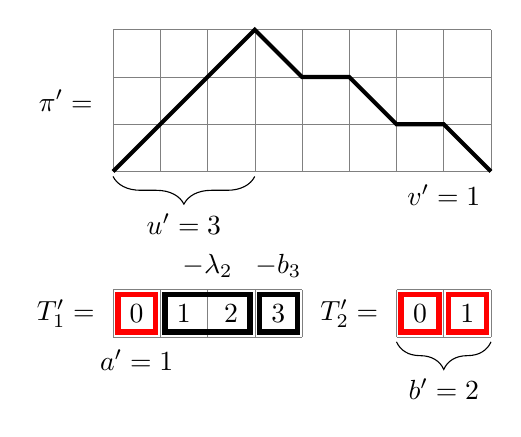
\begin{tikzpicture}[scale=0.6]
  \draw[help lines] (0,0) grid (8,3);
\draw[line width = 1.5pt] (0,0) -- ++(1,1) -- ++(1,1) -- ++(1,1) -- ++(1,-1) -- ++(1,0) -- ++(1,-1) -- ++(1,0) -- ++(1,-1);
  \draw [decorate,decoration={brace,amplitude=10pt},xshift=-0pt,yshift=-3pt]
(3,0) -- (0,0) node [black,midway,yshift=-0.6cm] {\( u'=3 \)};
\node at (-1,1.5) {\( \pi'= \)};
\remove(1,1)
\node at (7,-.5) {\( v'=1 \)};
\begin{scope}[shift={(0,-3.5)}]
  \draw [help lines] (0,0) grid (4,1);
  \foreach \x in {0,...,3} \draw node at (\x+0.5,0.5) {\x};
  \RM0 \BD2 \BM3
\node at (-1,.5) {\( T'_1= \)};
\node at (.5,-.5) {\( a'=1 \)};
\node at (3.5,1.5) {\( -b_3 \)};
\node at (2,1.5) {\( -\lambda_2 \)};
\end{scope}
\begin{scope}[shift={(6,-3.5)}]
  \draw [help lines] (0,0) grid (2,1);
  \foreach \x in {0,...,1} \draw node at (\x+0.5,0.5) {\x};
  \RM0 \RM1
  \draw [decorate,decoration={brace,amplitude=10pt},xshift=-0pt,yshift=-3pt]
(2,0) -- (0,0) node [black,midway,yshift=-0.6cm] {\( b'=2 \)};
\node at (-1,.5) {\( T'_2= \)};
\end{scope}
\end{tikzpicture}  
\caption{A triple \( (\pi,T_1,T_2)\in X \) in Case 1-2 on the left and
  the corresponding triple \( (\pi',T'_1,T'_2)\in X \) in Case 2-2 on
  the right, where \( r=4 \), \( s=2 \), and \( n=5 \). The peak (an
  upstep followed by a down step) \( (1,1)\to (2,2)\to(3,1) \) in
  \( \pi \) is collapsed to a point.}
  \label{fig:case-2}
\end{figure}

\begin{figure}
  \centering
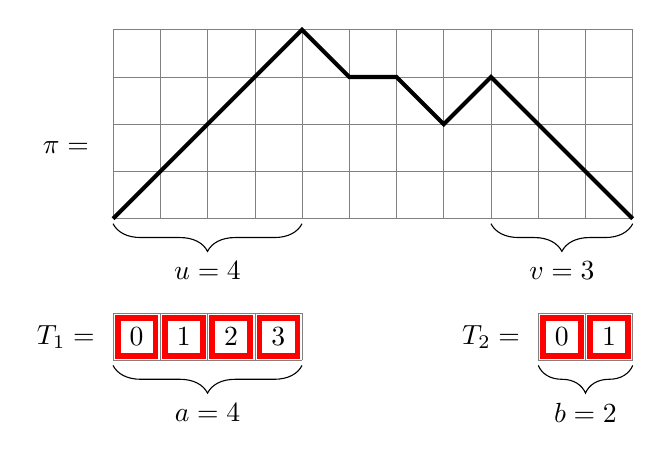
\begin{tikzpicture}[scale=0.6]
  \draw[help lines] (0,0) grid (11,4);
\draw[line width = 1.5pt] (0,0) -- ++(1,1) -- ++(1,1) -- ++(1,1) -- ++(1,1) -- ++(1,-1) -- ++(1,0) -- ++(1,-1) -- ++(1,1) -- ++(1,-1) -- ++(1,-1) -- ++(1,-1);
  \draw [decorate,decoration={brace,amplitude=10pt},xshift=-0pt,yshift=-3pt]
(4,0) -- (0,0) node [black,midway,yshift=-0.6cm] {\( u=4 \)};
\node at (-1,1.5) {\( \pi= \)};
  \draw [decorate,decoration={brace,amplitude=10pt},xshift=-0pt,yshift=-3pt]
(11,0) -- (8,0) node [black,midway,yshift=-0.6cm] {\( v=3 \)};
\begin{scope}[shift={(0,-3)}]
  \draw [help lines] (0,0) grid (4,1);
  \foreach \x in {0,...,3} \draw node at (\x+0.5,0.5) {\x};
  \RM0 \RM1 \RM2 \RM3
  \draw [decorate,decoration={brace,amplitude=10pt},xshift=-0pt,yshift=-3pt]
(4,0) -- (0,0) node [black,midway,yshift=-0.6cm] {\( a=4 \)};
\node at (-1,.5) {\( T_1= \)};
\end{scope}
\begin{scope}[shift={(9,-3)}]
  \draw [help lines] (0,0) grid (2,1);
  \foreach \x in {0,...,1} \draw node at (\x+0.5,0.5) {\x};
  \RM0 \RM1
  \draw [decorate,decoration={brace,amplitude=10pt},xshift=-0pt,yshift=-3pt]
(2,0) -- (0,0) node [black,midway,yshift=-0.6cm] {\( b=2 \)};
\node at (-1,.5) {\( T_2= \)};
\end{scope}
\end{tikzpicture}
\caption{A triple \( (\pi,T_1,T_2)\in X \) in Case 5, where \( r=4 \),
  \( s=2 \), and \( n=5 \).}
  \label{fig:case5}
\end{figure}

By the construction, Case 1 corresponds to Case 2 and Case 3
corresponds to Case 4. Thus the map
\( \phi(T_1,T_2,\pi)= (T'_1,T'_2,\pi') \) is a sign-reversing
weight-preserving involution on \( X \) with fixed points
\( (\emptyset,\emptyset,\pi) \) where \( \pi\in Y \). This completes
the proof.
\end{proof}

\chapter{Moments of classical orthogonal polynomials}

In this chapter we apply the combinatorial interpretation of moments
for Tchebyshev polynomials of the 1st and 2nd kinds, Hermite
polynomials, Charlier polynomials, and Laguerre polynomials.

Note that a monic OPS \( \{ P_n(x) \}_{n\ge 0} \) can be defined in
many ways, namely, one of the following determines the orthogonal
polynomials:
\begin{enumerate}
\item the coefficients \( \{a_{n,k}\}_{n,k\ge0} \) of \( P_n(x)= \sum_{k=0}^{n} a_{n,k} x^k   \),
\item the generating function \( \sum_{n\ge0}P_n(x)t^n \)
  or \( \sum_{n\ge0}P_n(x)t^n/n! \),
\item the moments \( \{ \mu_n\}_{n\ge 0} \),
\item the 3-term recurrence coefficients \( \{ b_n\}_{n\ge 0} \) and
  \( \{ \lambda_n\}_{n\ge 1} \).
\end{enumerate}

\section{Tchebyshev polynomials}

In this section we will compute the moments of Tchebyshev polynomials
using \Cref{thm:mu=Mot}. We will first consider Tchebyshev polynomials
of the second kind since they are simpler than the first kind in our
approach.



The \emph{Tchebyshev polynomials of the second kind}
\( U_n(x) \) are defined by
\[
  U_n(x) = \frac{\sin(n+1)\theta}{\sin\theta}, \qquad x=\cos\theta,
  \qquad n\ge0.
\]
They satisfy
  \[
    U_{n+1}(x) = 2x U_n(x) - U_{n-1}(x), \qquad n\ge0,
  \]
  where \( U_{-1}(x) = 0 \) and \( U_0(x) = 1 \).
  Using calculus we can prove that
  \[
    \int_{-1}^1 U_m(x)U_n(x) (1-x^2)^{1/2} dx = \frac{\pi}{2}\delta_{m,n}.
  \]
  Let \( \LL \) be the linear functional defined by
  \[
    \LL(f(x)) = \frac{2}{\pi} \int_{-1}^1 f(x) (1-x^2)^{1/2} dx.
  \]
  Then \( \{U_n(x)\}_{n\ge0} \) is an OPS for \( \LL \) and
  \( \LL(1) = 1 \).

  Since \( U_n(x) \) has leading coefficient \( 2^n \), the monic
  Tchebyshev polynomials \( \hat{U}_n(x) \) are given by
  \( \hat{U}_n(x) = 2^{-n}U_n(x) \) and
  \[
    \hat{U}_{n+1}(x) = (x-b_n) \hat{U}_n(x) - \lambda_n \hat{U}_{n-1}(x), \qquad n\ge0,
  \] 
  where \( b_n = 0 \) and \( \lambda_n = 1/4 \).

  Note that \( \{\hat{U}_n(x)\}_{n\ge0} \) is also an OPS for
  \( \LL \). Using calculus we can prove that
  the moments
  \[
    \mu_n= \LL(x^n) = \frac{2}{\pi} \int_{-1}^1 x^n (1-x^2)^{1/2} dx
  \]
  are given by
  \begin{equation}\label{eq:20}
    \mu_{2n} = \frac{1}{4^n} C_n, \qquad \mu_{2n+1} = 0.
  \end{equation}
  We will prove this combinatorially using the combinatorial
  interpretation for \( \mu_n \).

  By \Cref{thm:mu=Mot},
  \[
    \mu_n = \sum_{\pi\in \Motz_n} \wt(\pi)
    = \sum_{\pi\in \Dyck_n} \left( \frac{1}{4} \right)^{n/2}.
  \]
  Thus
  \[
    \mu_{2n} = \frac{1}{4^n} |\Dyck_{2n}|, \qquad \mu_{2n+1} = 0.
  \]
  This is the same as \eqref{eq:20}.

  \medskip

  Now we consider the Tchebyshev polynomials of the first kind,
  \( T_n(x) = \cos n\theta \), \( x=\cos \theta \). Recall that
\[
  \int_{-1}^1 T_m(x)T_n(x) (1-x^2)^{-1/2} dx = 0, \qquad m\ne n.
\]
  Let \( \LL \) be the linear functional defined by
  \[
    \LL(f(x)) = \frac{1}{\pi} \int_{-1}^1 f(x) (1-x^2)^{-1/2} dx.
  \]
  Then \( \{T_n(x)\}_{n\ge0} \) is an OPS for \( \LL \) and
  \( \LL(1) = 1 \). The moments
  \[
    \mu_n= \LL(x^n) = \frac{1}{\pi} \int_{-1}^1 x^n (1-x^2)^{-1/2} dx
  \]
  are given by
  \begin{equation}\label{eq:21}
    \mu_{2n} = \frac{1}{2^{2n}} \binom{2n}{n}, \qquad
    \mu_{2n+1} = 0.
  \end{equation}
  We will prove this combinatorially.

  The monic Tchebyshev polynomials of the first kind are given by
  \( \hat{T}_0(x) = 1 \) and \( \hat{T}_n(x) = 2^{1-n}T_n(x) \) for
  \( n\ge1 \). We have
  \[
      \hat{T}_{n+1}(x) = (x-b_n) \hat{T}_n(x) - \lambda_n\hat{T}_{n-1}(x),
      \qquad n\ge0,
  \]
  where \( b_n=0 \) for \( n\ge0 \), \( \lambda_1 = 1/2 \), and
  \( \lambda_n = 1/4 \) for \( n\ge2 \).


  By \Cref{thm:mu=Mot},
  \[
    \mu_n = \sum_{\pi\in \Motz_n} \wt(\pi)
    = \left( \frac{1}{4} \right)^{n/2} \sum_{\pi\in \Dyck_n} 2^{a(\pi)},
  \]
  where \( a(\pi) \) is the number of down steps in \( \pi \) touching
  the \( x \)-axis. Thus \eqref{eq:21} is a consequence of the
  following proposition.

  \begin{prop}
    We have
    \begin{equation}\label{eq:22}
     \sum_{\pi\in \Dyck_{2n}} 2^{a(\pi)} = \binom{2n}{n}.
   \end{equation}
  \end{prop}

  \begin{proof}
    Define a \emph{colored Dyck path} to be a Dyck path in
    \( \Dyck_{2n} \) such that every down step touching the
    \( x \)-axis is colored red or black. The left-hand side of the
    equation is the number of colored Dyck paths in \( \Dyck_{2n} \).
    Thus it suffices to show that this number is equal to
    \( \binom{2n}{n} \).

    Note that every Dyck path \( \pi\in \Dyck_{2n} \) is decomposed into
    \[
      \pi = (U\pi_1 D) (U \pi_2 D) \cdots (U\pi_k D),
    \]
    where \( \pi_i\in \Dyck_{2t_i} \) for some
    \( t_i\in \ZZ_{\ge0} \). Each down step \( D \) after \( \pi_i \)
    touches the \( x \)-axis and no other down steps have this
    property. Thus a colored Dyck path
    can be identified with a sequence of the form
    \[
      \pi = (U\pi_1 D_1) (U \pi_2 D_2) \cdots (U\pi_k D_k),
    \]
    where each \( D_i \) is colored red or black. If \( D_i \) is
    colored red, reflect the subpath \( U\pi_iD \) about the
    \( x \)-axis. Then we get a path from \( (0,0) \) to \( (2n,0) \)
    consisting of up steps and down steps (which may go below the
    \( x \)-axis).

    \begin{figure}
      \centering
     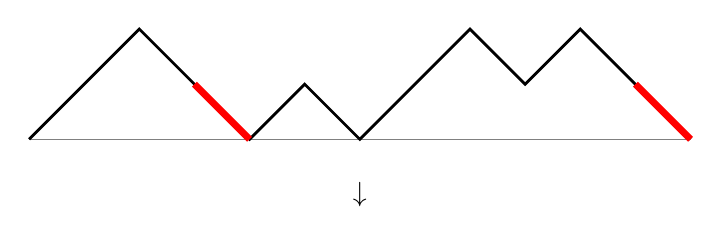
\begin{tikzpicture}[scale=.7]
\draw[help lines] (0,0) grid (12,0);
\draw[line width = 1pt] (0,0) -- ++(1,1) -- ++(1,1) -- ++(1,-1) -- ++(1,-1) -- ++(1,1) -- ++(1,-1) -- ++(1,1) -- ++(1,1) -- ++(1,-1) -- ++(1,1) -- ++(1,-1) -- ++(1,-1);
  \node at (6,-1) {\( \downarrow \)};
\draw[line width = 2.5pt,red] (3,1) -- (4,0);
\draw[line width = 2.5pt,red] (11,1) -- (12,0);
\end{tikzpicture}

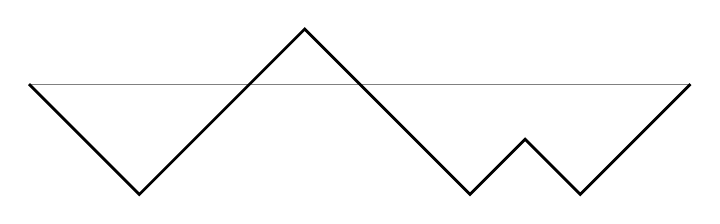
\begin{tikzpicture}[scale=.7]
\draw[help lines] (0,0) grid (12,0);
\draw[line width = 1pt] (0,0) -- ++(1,-1) -- ++(1,-1) -- ++(1,1) -- ++(1,1) -- ++(1,1) -- ++(1,-1) -- ++(1,-1) -- ++(1,-1) -- ++(1,1) -- ++(1,-1) -- ++(1,1) -- ++(1,1);
\end{tikzpicture}
      \caption{The map reflecting each path with a red down step.}
      \label{fig:reflect}
    \end{figure}


    This map gives a bijection between the colored Dyck paths from
    \( (0,0) \) to \( (2n,0) \) to any path from \( (0,0) \) to
    \( (2n,0) \) consisting of up steps and down steps. Since there
    are \( \binom{2n}{n} \) such paths, we obtain the result.
  \end{proof}
  

\section{Hermite polynomials}

The \emph{Hermite polynomials} \( H_n(x) \) are defined by
\( H_{-1}(x) = 0 \), \( H_{0}(x) = 1 \), and
\[
  H_{n+1}(x) = 2x H_n(x) - 2n H_{n-1}(x), \qquad  n\ge1.
\]
Since the leading coefficient of \( H_n(x) \) is \( 2^n \), we can
make it monic by letting \( \hat{H}_n(x) = 2^{-n}H_n(x) \). Then
\( \hat{H}_{-1}(x) = 0 \), \( \hat{H}_{0}(x) = 1 \), and
\begin{equation}\label{eq:25}
  \hat{H}_{n+1}(x) = x \hat{H}_n(x) - \frac{n}{2} \hat{H}_{n-1}(x), \qquad  n\ge1.
\end{equation}

For the combinatorial study of orthogonal polynomials, it is more
convenient if the recurrence coefficients \( b_n \) and
\( \lambda_n \) are integers. We can rescale orthogonal polynomials
using the following lemma.

\begin{lem}[Rescaling OPS] \label{lem:rescaling} 
  Suppose that \( \{ P_n(x) \}_{n\ge 0} \) is a monic OPS such that
  \( P_{-1}(x) = 0 \), \( P_{0}(x) = 1 \), and
  \begin{equation}\label{eq:23}
      P_{n+1}(x) = (x-b_n) P_n(x) - \lambda_n P_{n-1}(x), \qquad n\ge1.
  \end{equation}
  Let \( \widetilde{P}_n(x) = a^n P_n(x/a) \), where \( a\ne0 \). Then
  \( \widetilde{P}_{-1}(x) = 0 \), \( \widetilde{P}_{0}(x) = 1 \), and
  \begin{equation}\label{eq:24}
    \widetilde{P}_{n+1}(x) = (x-ab_n) \widetilde{P}_n(x) - a^2\lambda_n
    \widetilde{P}_{n-1}(x), \qquad n\ge1.
  \end{equation}
\end{lem}
\begin{proof}
  Replacing \( x \) by \( x/a \) and multiplying both sides by
  \( a^{n+1} \) in \eqref{eq:23} yields \eqref{eq:24}.
\end{proof}

Define the \emph{rescaled Hermite polynomials}
\( \widetilde{H}_n(x) \) by
\( \widetilde{H}_n(x) = \sqrt{2}^n \hat{H}_n(x/\sqrt{2}) \). By
\Cref{lem:rescaling} and \eqref{eq:25},
\( \widetilde{H}_{-1}(x) = 0 \), \( \widetilde{H}_1(x) = 1 \), and 
\begin{equation}\label{eq:hermite-3rr}
  \widetilde{H}_{n+1}(x) = x \widetilde{H}_n(x) - n
  \widetilde{H}_{n-1}(x), \qquad n\ge1.
\end{equation}

We note that \( H_n(x) \) are called ``physicist's Hermite
polynomials'' and \( \widetilde{H}_n(x) \) are called ``probabilist's
Hermite polynomials''.

The moment \( \mu_n \) of \( \{ \widetilde{H}_n(x) \}_{n\ge 0} \) 
is given by
\[
  \mu_n = \sum_{\pi\in\Motz_n} \wt(\pi),
\]
where \( \wt(\pi) \) is determined by \( b_n=0 \) and
\( \lambda_n=n \). Since \( b_n=0 \),
we have \( \mu_{2n+1}=0 \) and
\[
  \mu_{2n} = \sum_{\pi\in\Dyck_{2n}} \wt(\pi).
\]
Note that for each \( \pi\in\Dyck_{2n} \), its weight \( \wt(\pi) \)
is a positive integer. It is thus natural to ask what combinatorial
objects \( \wt(\pi) \) counts.

\begin{defn}
  A \emph{Hermite history} is a Dyck path where each down step
  starting at height \( k \) has a label in \( \{1,\dots,k\} \).
  Let \( \HH_{2n} \) denote the set of Hermite histories whose
  underlying Dyck paths are from \( (0,0) \) to \( (2n,0) \).
\end{defn}

Let \( \pi\in\Dyck_{2n} \). For each down step of \( \pi \) starting
at height \( k \), there are \( k \) ways to assign a label from
\( \{1,\dots,k\} \). Thus \( \wt(\pi) \) is the number of Hermite
histories with underlying Dyck path \( \pi \). This implies
\( \mu_{2n} = |\HH_{2n}|  \).

Let \( \CM_{2n} \) be the set of complete matchings on \( [2n] \).

\begin{prop}
  There is a bijection between \( \HH_{2n} \) and \( \CM_{2n} \).
\end{prop}

\begin{proof}
  Let \( \pi\in \HH_{2n} \). We construct a complete matching
  \( \rho \) as follows. For \( k= 1,\dots,2n \), if the \( k \)th
  step of \( \pi \) is an up step, then make the \( k \)th vertex of
  \( \rho \) to be an \emph{opener}, which means it will be connected
  to a vertex to its right. If the \( k \)th step of \( \pi \) is a
  down step, then make the \( k \)th vertex of \( \rho \) to be a
  \emph{closer}, which means it will be connected to a vertex to its
  left. If the \( k \)th step of \( \pi \) is a down step with label
  \( a_k \), then connected the vertex at \( k \) with the \( k \)th
  closest available opener. For example, see
  \Cref{fig:Hermite-history}.

  Observe that the height of the starting point of the \( k \)th down
  step is equal to the number of available openers for the vertex
  \( k \). Therefore the map \( \pi\mapsto \rho \) is well-defined.
  The inverse map \( \rho\mapsto \pi \) is straighforward to
  construct. Hence the map \( \pi\mapsto \rho \) is a bijection from
  \( \HH_{2n} \) and \( \CM_{2n} \).
\end{proof}

\begin{figure}
  \centering
 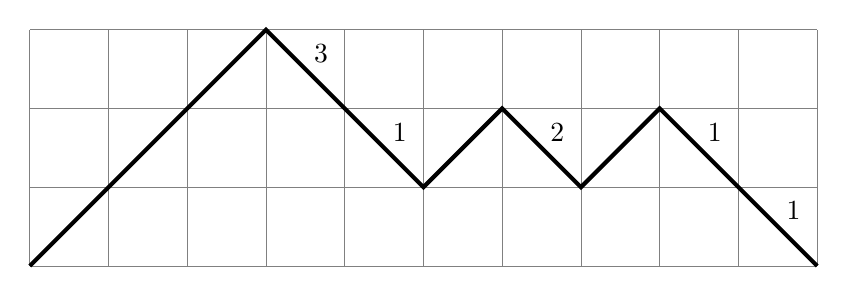
\begin{tikzpicture}
\draw[help lines] (0,0) grid (10,3);
\draw[line width = 1.5pt] (0,0) -- ++(1,1) -- ++(1,1) -- ++(1,1) -- ++(1,-1) -- ++(1,-1) -- ++(1,1) -- ++(1,-1) -- ++(1,1) -- ++(1,-1) -- ++(1,-1);
\node at (3.7,2.7) {3};
\node at (4.7,1.7) {1};
\node at (6.7,1.7) {2};
\node at (8.7,1.7) {1};
\node at (9.7,0.7) {1};
\end{tikzpicture}

\begin{tikzpicture}
\begin{scope}[shift={(0,0)}]
\node (0,0) at (1,1) {};
\draw (1,0) -- (1.3,0.3);
\draw (2,0) -- (2.3,0.3);
\draw (3,0) -- (3.3,0.3);
\draw (4,0) -- (3.7,0.3);
\draw (5,0) -- (4.7,0.3);
\draw (6,0) -- (6.3,0.3);
\draw (7,0) -- (6.7,0.3);
\draw (8,0) -- (8.3,0.3);
\draw (9,0) -- (8.7,0.3);
\draw (10,0) -- (9.7,0.3);
\node[draw,circle,fill=white] (1) at (1,0) {};
\node[draw,circle,fill=white] (4) at (4,0) {};
\node[draw,circle,fill=white] (2) at (2,0) {};
\node[draw,circle,fill=white] (7) at (7,0) {};
\node[draw,circle,fill=white] (3) at (3,0) {};
\node[draw,circle,fill=white] (5) at (5,0) {};
\node[draw,circle,fill=white] (6) at (6,0) {};
\node[draw,circle,fill=white] (10) at (10,0) {};
\node[draw,circle,fill=white] (8) at (8,0) {};
\node[draw,circle,fill=white] (9) at (9,0) {};
\end{scope}
\end{tikzpicture}

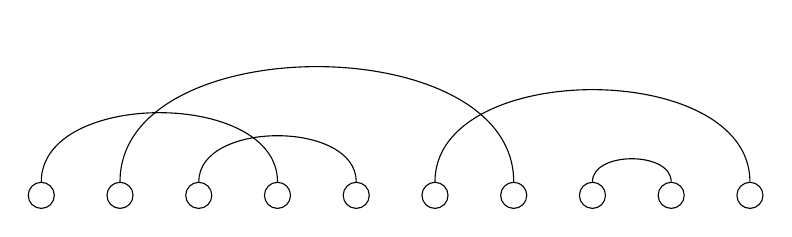
\begin{tikzpicture}
\begin{scope}[shift={(0,0)}]
\node (0.5) at (1,0) {};
\node[draw, circle] (1) at (1,0) {};
\node[draw, circle] (4) at (4,0) {};
\draw[out=90,in=90] (1) to (4);
\node[draw, circle] (2) at (2,0) {};
\node[draw, circle] (7) at (7,0) {};
\draw[out=90,in=90] (2) to (7);
\node[draw, circle] (3) at (3,0) {};
\node[draw, circle] (5) at (5,0) {};
\draw[out=90,in=90] (3) to (5);
\node[draw, circle] (6) at (6,0) {};
\node[draw, circle] (10) at (10,0) {};
\draw[out=90,in=90] (6) to (10);
\node[draw, circle] (8) at (8,0) {};
\node[draw, circle] (9) at (9,0) {};
\draw[out=90,in=90] (8) to (9);
\end{scope}
\end{tikzpicture}
\caption{A Hermite history (top), the openers and closers (middle),
  and the corresponding matching (bottom).}
  \label{fig:Hermite-history}
\end{figure}

Since the number of complete matchings on \( [2n] \) is
\( (2n-1)!! \), we obtain the following result.

\begin{cor}
  The \( 2n \)th moment of rescaled Hermite polynomials
  \( \widetilde{H}_n(x) \) is
  \[
    \mu_{2n} = (2n-1)!!.
  \]
\end{cor}


\section{Charlier polynomials}

The (normalized) \emph{Charlier polynomials}
\( C_n(x;a) \) are defined by
\( C_{-1}(x;a) =0 \), \( C_{1}(x;a) =1 \), and
\[
  C_{n+1}(x;a) = (x-n-a) C_n(x;a) - an C_{n-1}(x;a), \qquad n\ge1.
\]

\begin{defn}
  A \emph{Charlier history} is a Motzkin path where each horizontal
  step at height \( k \) has a label in \( \{0,1,\dots,k\} \) and each
  down step starting at height \( k \) has a label in
  \( \{1,\dots,k\} \). Let \( \CH_{n} \) denote the set of
  Charlier histories whose underlying Motzkin paths are from
  \( (0,0) \) to \( (n,0) \).
  For \( \rho\in \CH_{n} \), define \( t(\rho) \)
  to the number of horizontal steps with label \( 0 \)
  plus the number of down steps.
\end{defn}

Since \( b_k = k+a \) and \( \lambda_k = ak \), by the definition of
the Charlier histories, the moment \( \mu_n \) of the Charlier
polynomials is given by
\[
  \mu_n = \sum_{\pi\in \Motz_n} \wt(\pi) = \sum_{\rho\in \CH_n}
  a^{t(\rho)}.
\]

For a set partition \( \sigma \), let \( \block(\sigma) \) denote the
number of blocks in \( \sigma \).

\begin{thm}
  The moment \( \mu_n \) of the Charlier polynomials is given by
\[
  \mu_n = \sum_{\sigma\in \Pi_n} a^{\block(\sigma)}.
\]
\end{thm}

\begin{proof}
  We will construct a weight-preserving bijection
  \( \phi:\CH_n\to \Pi_n \). Let \( \rho\in \CH_n \). We construct the
  corresponding set partition \( \phi(\rho) = \sigma\in\Pi_n \) as
  follows. For \( k= 1,\dots,n \),
\begin{itemize}
\item if the \( k \)th step of \( \rho \) is an up step, then make the
  \( k \)th vertex of \( \sigma \) to be an opener,
\item if the \( k \)th step of \( \rho \) is a down step, then make
  the \( k \)th vertex of \( \rho \) to be a closer,
\item if the \( k \)th step of \( \rho \) is a horizontal step, then
  make the \( k \)th vertex of \( \rho \) to be a \emph{transient},
  which means that it is connected to a vertex to its left and also a
  vertex to its right.
\end{itemize}
If the \( k \)th step of \( \rho \) is a down step with label
\( a_k \), then connected the vertex at \( k \) with the \( k \)th
closest available opener or transient. If the \( k \)th step of
\( \rho \) is a horizontal step with label \( a_k \), then connected
the vertex at \( k \) with the \( k \)th closest available opener or
transient. Here, if \( a_k=0 \), we the vertex \( k \) is connected to
itself making it a singleton. For example, see
\Cref{fig:Charlier-history}.

It is not hard to see that \( \phi:\CH_n\to \Pi_n \) is a bijection.
Moreover, if \( \phi(\rho) = \sigma \), then
\( t(\rho) = \block(\sigma) \). This can be seen from the observation
that every block of \( \rho \) is either a singleton (corresponding to
a horizontal step with label \( 0 \)) or a block with exactly one
closer (corresponding to a down step). This completes the proof.
\end{proof}

\begin{figure}
  \centering
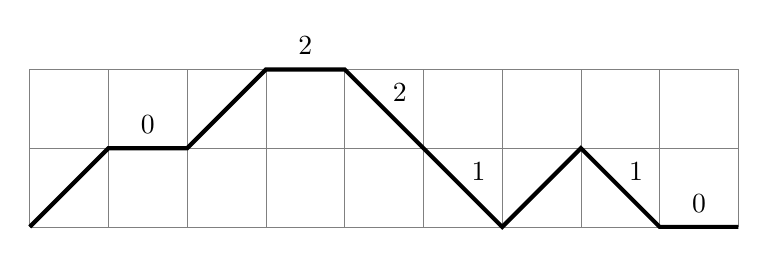
\begin{tikzpicture}
\draw[help lines] (0,0) grid (9,2);
\draw[line width = 1.5pt] (0,0) -- ++(1,1) -- ++(1,0) -- ++(1,1) -- ++(1,0) -- ++(1,-1) -- ++(1,-1) -- ++(1,1) -- ++(1,-1) -- ++(1,0);
\node at (1.5,1.3) {0};
\node at (3.5,2.3) {2};
\node at (4.7,1.7) {2};
\node at (5.7,0.7) {1};
\node at (7.7,0.7) {1};
\node at (8.5,0.3) {0};
\end{tikzpicture}
 
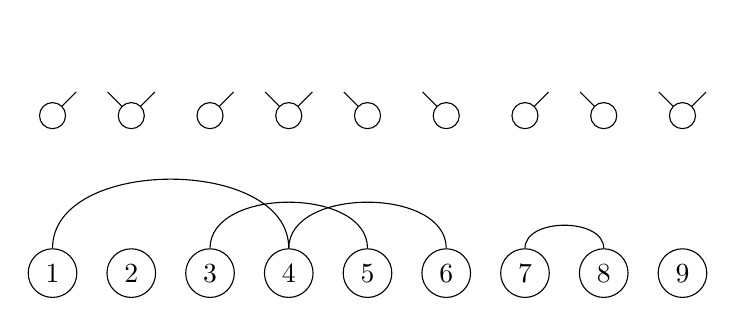
\begin{tikzpicture}
\begin{scope}[shift={(0,0)}]
\node (0,0) at (1,1) {};
\draw (1,0) -- (1.3,0.3);
\draw (1.7,0.3) -- (2,0) -- (2.3,0.3);
\draw (3,0) -- (3.3,0.3);
\draw (3.7,0.3) -- (4,0) -- (4.3,0.3);
\draw (5,0) -- (4.7,0.3);
\draw (6,0) -- (5.7,0.3);
\draw (7,0) -- (7.3,0.3);
\draw (8,0) -- (7.7,0.3);
\draw (8.7,0.3) -- (9,0) -- (9.3,0.3);
\node[draw,circle,fill=white] (1) at (1,0) {};
\node[draw,circle,fill=white] (4) at (4,0) {};
\node[draw,circle,fill=white] (2) at (2,0) {};
\node[draw,circle,fill=white] (7) at (7,0) {};
\node[draw,circle,fill=white] (3) at (3,0) {};
\node[draw,circle,fill=white] (5) at (5,0) {};
\node[draw,circle,fill=white] (6) at (6,0) {};
\node[draw,circle,fill=white] (8) at (8,0) {};
\node[draw,circle,fill=white] (9) at (9,0) {};
\end{scope}
\begin{scope}[shift={(0,-2)}]
\node[draw, circle] (1) at (1,0) {\( 1 \)};
\node[draw, circle] (4) at (4,0) {\( 4 \)};
\node[draw, circle] (6) at (6,0) {\( 6 \)};
\draw[out=90,in=90] (1) to (4);
\draw[out=90,in=90] (4) to (6);
\node[draw, circle] (2) at (2,0) {\( 2 \)};
\node[draw, circle] (3) at (3,0) {\( 3 \)};
\node[draw, circle] (5) at (5,0) {\( 5 \)};
\draw[out=90,in=90] (3) to (5);
\node[draw, circle] (7) at (7,0) {\( 7 \)};
\node[draw, circle] (8) at (8,0) {\( 8 \)};
\draw[out=90,in=90] (7) to (8);
\node[draw, circle] (9) at (9,0) {\( 9 \)};
\end{scope}
\end{tikzpicture}

\caption{A Charlier history (top), the openers, closers, and
  transients (middle), and the corresponding set partition (bottom).}
  \label{fig:Charlier-history}
\end{figure}


\section{Laguerre polynomials}

The (normalized) \emph{Laguerre polynomials} \( L^{(\alpha)}_n(x) \)
are defined by\footnote{In the literature it is more common to define
  the Laguerre polynomials with \( \alpha \) replaced by
  \( \alpha+1 \) in our definition.} \( L^{(\alpha)}_{-1}(x) =0 \),
\( L^{(\alpha)}_{1}(x) =1 \), and
\[
  L^{(\alpha)}_{n+1}(x) = (x-2n-\alpha) L^{(\alpha)}_n(x) - n(n-1+\alpha) L^{(\alpha)}_{n-1}(x), \qquad n\ge1.
\]


\begin{lem}\label{lem:1}
  Suppose that \( \{ P_n(x) \}_{n\ge 0} \) is a monic OPS such that
  \[
    P_{n+1}(x) = (x-b_n) P_n(x) - a_{n-1}c_n P_{n-1}(x).
  \]
  Then
  \[
    \mu_n = \sum_{\pi\in \Motz_n} \wt'(\pi),
  \]
  where \( \wt'(\pi) \) is the product of the weights of the steps in \( \pi \) and
  \begin{itemize}
  \item the weight of an up step starting at height \( k \) is \( a_k \),
  \item the weight of a horizontal step at height \( k \) is \( b_k \),
  \item the weight of a down step starting at height \( k \) is \( c_k \).
  \end{itemize}
\end{lem}

\begin{proof}
  We know that
  \[
    \mu_n = \sum_{\pi\in \Motz_n} \wt(\pi),
  \]
  where \( \wt(\pi) \) is the product of \( b_k \) for each horizontal
  step of height \( k \) and \( \lambda_k = a_kc_k \) for each down
  step starting at height \( k \). Observe that for
  \( \pi\in \Motz_n \) every down step corresponds to a unique up
  step. More precisely, if we write \( \pi \) as a sequence of steps
  \( S_1 \cdots S_n \) and if \( S_i = D \), then there is a unique
  index \( j \) such that \( S_j=U \) and \( S_{j+1}\cdots S_{i-1} \)
  is a (translated) Dyck path in \( \Dyck_{i-j-1} \).

Thus we can split the weight \( \lambda_k=a_kc_k \) on a down
  step starting at height \( k \) into the weight \( a_k \) of the
  corresponding up step and the weight \( c_k \) of the down step as
  shown in \Cref{fig:up-down}. This proves the lemma.
  \begin{figure}
    \centering
    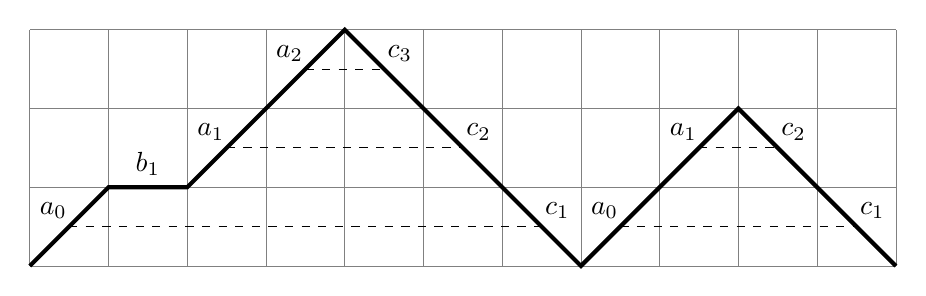
\begin{tikzpicture}
\draw[help lines] (0,0) grid (11,3);
\draw[line width = 1.5pt] (0,0) -- ++(1,1) -- ++(1,0) -- ++(1,1) -- ++(1,1) -- ++(1,-1) -- ++(1,-1) -- ++(1,-1) -- ++(1,1) -- ++(1,1) -- ++(1,-1) -- ++(1,-1);
\draw[dashed] (0.5,0.5) -- (6.5,0.5);
\draw[dashed] (2.5,1.5) -- (5.5,1.5);
\draw[dashed] (3.5,2.5) -- (4.5,2.5);
\draw[dashed] (7.5,0.5) -- (10.5,0.5);
\draw[dashed] (8.5,1.5) -- (9.5,1.5);
\node at (0.3,0.7) {\( a_0 \)};
\node at (1.5,1.3) {\( b_1 \)};
\node at (2.3,1.7) {\( a_1 \)};
\node at (3.3,2.7) {\( a_2 \)};
\node at (4.7,2.7) {\( c_3 \)};
\node at (5.7,1.7) {\( c_2 \)};
\node at (6.7,0.7) {\( c_1 \)};
\node at (7.3,0.7) {\( a_0 \)};
\node at (8.3,1.7) {\( a_1 \)};
\node at (9.7,1.7) {\( c_2 \)};
\node at (10.7,0.7) {\( c_1 \)};
\end{tikzpicture}
\caption{Splitting the weight \( \lambda_k=a_{k-1}c_k \)
  into \( a_{k-1} \) and \( c_k \).}
    \label{fig:up-down}
  \end{figure}
\end{proof}

By \Cref{lem:1}, the moment of the Laguerre polynomials is given by
\begin{equation}\label{eq:26}
    \mu_n = \sum_{\pi\in \Motz_n} \wt'(\pi),
\end{equation}
where \( a_k = k+\alpha \), \( b_k = 2k+\alpha \), and
\( c_k = k \).


\begin{defn}
  A \emph{Laguerre history} is a Motzkin path where 
\begin{itemize}
\item each up step starting at height \( k \)
  has a label in \( \{0,1,\dots,k\} \),
\item each horizontal step at height \( k \) has a label in
  \( \{-k,\dots,-1,0,1,\dots,k\} \),
\item  each down step starting at height \( k \)
  has a label in \( \{1,2,\dots,k\} \),
\end{itemize}

Let \( \LH_{n} \) denote the set of Laguerre histories whose
underlying Motzkin paths are from \( (0,0) \) to \( (n,0) \). For
\( \rho\in \LH_{n} \), define \( \zero(\rho) \) to be the
number of labels equal to \( 0 \) in \( \rho \).
\end{defn}

Then \eqref{eq:26} is equivalent to
\[
  \mu_n = \sum_{\rho\in \LH_n} \alpha^{\zero(\rho)}.
\]

There are several bijections between \( \sym_n \) and \( \LH_n \) due
to Fran\c{c}on--Viennot \cite{Francon1979}, Foata--Zeilberger
\cite{Foata1990a}, see also \cite[Algorithm~7]{Corteel2020a}. To prove
the following theorem we use a slight modification of the bijection
due to Fran\c{c}on--Viennot \cite{Francon1979}.

\begin{thm}\label{thm:Lag-mom}
We have
\[
  \mu_n = \sum_{\pi\in \sym_n} \alpha^{\cycle(\pi)}.
\]
\end{thm}

\begin{proof}
  It suffices to find a bijection \( \phi:\LH_n\to \sym_n \) such that
  if \( \phi(\rho)=\pi \), then 
  \( \zero(\rho) = \cycle(\pi) \). Consider
  \( \pi \in \LH_n \) and let \( S_k \) be the \( k \)th step of
  \( \pi \) and let \( \ell_k \) be its label.

For each \( k= 0,1,\dots,n \), we will construct a list \( A_k \) of
cycles of integers and dots, \( \fcirc \)'s. First we set
\( A_0 = \emptyset \). We then construct \( A_{k} \) recursively as follows.
\begin{description}
\item[Case 1:] \( S_k \) is an up step.
  \begin{description}
  \item[Case 1-1:] \( \ell_k=0 \). Create a new
  cycle ``\( (k\fcirc) \)'' at the beginning:
  \[
    A_k = (k\fcirc) A_{k-1}.
  \]
\item[Case 1-2:] \( \ell_k=i>0 \). Replace the
  \( i \)th dot in \( A_{k-1} \) by ``\( \fcirc k \fcirc \)''.
  \end{description}
\item[Case 2:] \( S_k \) is a horizontal step.
  \begin{description}
  \item[Case 2-1:] \( \ell_k=0 \). Create a new cycle ``\( (k) \)'' at the
    beginning:
  \[
    A_k = (k) A_{k-1}.
  \]
\item[Case 2-2:] \( \ell_k=i>0 \). Replace the \( i \)th dot in
  \( A_{k-1} \) by ``\( k \fcirc \)''.
\item[Case 2-3:] \( \ell_k=-i<0 \). Replace the \( i \)th dot in
  \( A_{k-1} \) by ``\( \fcirc k \)''.
  \end{description}

\item[Case 3:] \( S_k \) is a down step. Then \( \ell_k=i>0 \).
  Replace the \( i \)th dot in \( A_{k-1} \) by ``\( k \)''.
\end{description}
Then we define \( \phi(\rho) \)
to the permutation \( \pi \) whose cycle decomposition
is \( A_n \).

\begin{figure}
  \centering
  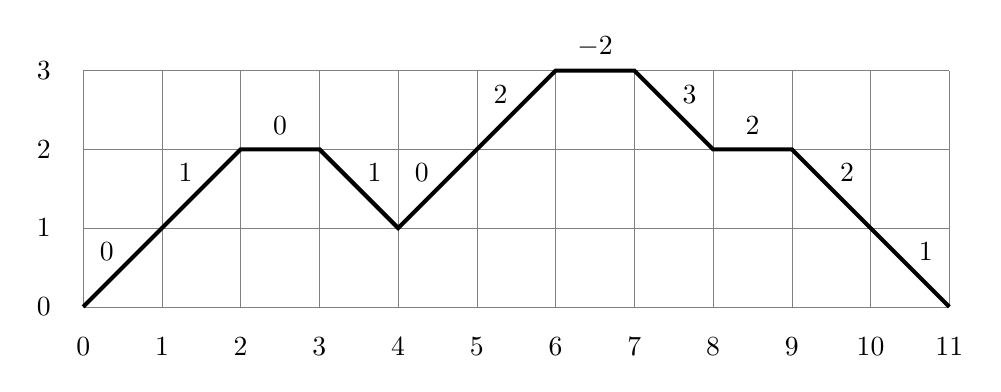
\begin{tikzpicture}
\draw[help lines] (0,0) grid (11,3);
\foreach \x in {0,...,11} \draw node at (\x,-.5) {\( \x \)};
\foreach \y in {0,...,3} \draw node at (-.5,\y) {\( \y \)};
\draw[line width = 1.5pt] (0,0) -- ++(1,1) -- ++(1,1) -- ++(1,0) -- ++(1,-1) -- ++(1,1) -- ++(1,1) -- ++(1,0) -- ++(1,-1) -- ++(1,0) -- ++(1,-1) -- ++(1,-1);
\node at (0.3,0.7) {\( 0 \)};
\node at (1.3,1.7) {\( 1 \)};
\node at (2.5,2.3) {\( 0 \)};
\node at (3.7,1.7) {\( 1 \)};
\node at (4.3,1.7) {\( 0 \)};
\node at (5.3,2.7) {\( 2 \)};
\node at (6.5,3.3) {\( -2 \)};
\node at (7.7,2.7) {\( 3 \)};
\node at (8.5,2.3) {\( 2 \)};
\node at (9.7,1.7) {\( 2 \)};
\node at (10.7,.7) {\( 1 \)};
\end{tikzpicture}
  \caption{A Laguerre history in \( \LH_{11} \).}
  \label{fig:Lag-his}
\end{figure}

For example, if \( \rho \) is the Laguerre history in \Cref{fig:Lag-his},
then
\begin{align*}
A_{0} &= \emptyset,\\
A_{1} &= (1,\fcirc),\\
A_{2} &= (1,\fcirc,2,\fcirc),\\
A_{3} &= (3),(1,\fcirc,2,\fcirc),\\
A_{4} &= (3),(1,4,2,\fcirc),\\
A_{5} &= (5,\fcirc),(3),(1,4,2,\fcirc),\\
A_{6} &= (5,\fcirc),(3),(1,4,2,\fcirc,6,\fcirc),\\
A_{7} &= (5,\fcirc),(3),(1,4,2,\fcirc,7,6,\fcirc),\\
A_{8} &= (5,\fcirc),(3),(1,4,2,\fcirc,7,6,8),\\
A_{9} &= (5,\fcirc),(3),(1,4,2,9,\fcirc,7,6,8),\\
A_{10} &= (5,\fcirc),(3),(1,4,2,9,10,7,6,8),\\
A_{11} &= (5,11),(3),(1,4,2,9,10,7,6,8).
\end{align*}

The number of dots in \( A_{k-1} \) is always equal to the ending
height, say \( h_{k-1} \), of \( S_1 \cdots S_{k-1} \). Since
\( h_{k-1} \) is the height of the starting point of \( S_k \), we
have \( |\ell_k|\le h_{k-1} \). Hence, if \( |\ell_k|=i \ne 0 \), we
can always find the \( i \)th dot in \( A_{k-1} \) and the above
construction is well defined.

We create a cycle if and only if \( \ell_k=0 \).
Thus, \( \zero(\rho) = \cycle(\pi) \) as desired.

To prove that the map \( \phi:\LH_n\to \sym_n \) is invertible, we
construct its inverse map. Let \( \pi\in \sym_n \). Then we write the
cycles of \( \sym_n \) so that each cycle starts with its smallest
element and the cycles are listed in the decreasing order of their
smallest elements. Let \( A_n \) be the list of cycles obtained in
this way. For \( k=n,n-1,\dots,1,0 \), we define \( A_{k-1} \) to be
the configuration obtained from \( A_k \) by replacing \( k \)
together with every dot ``\( \fcirc \)'' adjacent to it by a single
dot ``\( \fcirc \)''. If \( k \) forms a cycle of length \( 1 \), then
we delete the whole cycle ``\( (k)\)''. Once the sequence
\( A_0, A_1,\dots,A_n \) is constructed, we can define the
corresponding Laguerre history \( \rho \) whose \( k \)th step is
\( S_k \) with label \( \ell_k \) as follows.

For each \( k= 1,\dots,n \), we compare \( A_k \) with \( A_{k-1} \).
\begin{description}
\item[Case 1:] \( A_k = (k\fcirc) A_{k-1} \). Then define \( S_k=U \) and \( \ell_k=0 \).
\item[Case 2:] \( A_k \) is obtained from \( A_{k-1} \) by replacing
  the \( i \)th dot by ``\( \fcirc k \fcirc \)''. Then \( S_k=U \) and
  \( \ell_k=i \).
\item[Case 3:] \( A_k = (k) A_{k-1} \). Then define \( S_k=H \) and \( \ell_k=0 \).
\item[Case 4:] \( A_k \) is obtained from \( A_{k-1} \) by replacing
  the \( i \)th dot by ``\( k \fcirc \)''. Then \( S_k=D \) and
  \( \ell_k=i \).
\item[Case 5:] \( A_k \) is obtained from \( A_{k-1} \) by replacing
  the \( i \)th dot by ``\( \fcirc k \)''. Then \( S_k=D \) and
  \( \ell_k=-i \).
\end{description}
Then we define \( \psi(\pi) \) to be the resulting Laguerre history \( \rho \).

By the construction, \( \psi \) is the inverse map of \( \phi \), and
the proof is completed.
\end{proof}

By \Cref{thm:Lag-mom} and \eqref{eq:c(n,k)-gf}, we obtain the simple
formula for \( \mu_n \).

\begin{cor}
  The \( n \)th moment of Laguerre polynomials is
  \[
    \mu_n = \alpha(\alpha+1) \cdots (\alpha+n-1).
  \]
\end{cor}


Note that the bijection \( \phi:\LH_n\to \sym_n \)
induces two bijections \( \phi_1: \CH_n\to \Pi_n \)
and \( \phi_2: \HH_n\to \CM_n \).

To see this, observe that a Laguerre history becomes a Charlier
history if every up step has the zero label, and every horizontal step
has a nonnegative label. Then in the corresponding list \( A_n \) of
cycles, every cycle is an increasing list of integers. Hence the
cycles can be identified with blocks giving a set partition.

Similalry, a Laguerre history becomes a Hermite history if every up
step has the zero label, and there is no horizontal step. Then in the
corresponding list \( A_n \) of cycles, every cycle is a pair
\( (i,j) \) of integers \( i<j \). Hence the cycles can be identified
with arcs giving a complete matching.

\medskip

At this point the reader may wonder if there is another bijection between
Laguerre histories and permutations similar to the bijections in the
previous sections using arcs. Indeed, there is such a bijection due to
Foata and Zeilberger \cite{Foata1990a}. We will briefly describe this
bijection. For simplicity we consider the case \( \alpha=1 \). In this
map we use the usual Motzkin weight which gives a weight
\( b_k=2k+1 \) for a horizontal step starting at height \( k \) and a
weight \( \lambda_k=k^2 \) for a down step starting at height \( k \).

A \emph{modified Laguerre history} of length \( n \) is a Motzkin path
from \( (0,0) \) to \( (n,0) \) in which every horizontal step with
starting height \( k \) is labeled by an integer in
\( \{ -k,\dots,-1, 0, 1,\dots,k\} \) every down step with starting
height \( k \) is labeled by a pair \( (i,j) \) of integers in
\( \{ 1,\dots,k\} \).

Let \( \rho \) be a modified Laguerre history. For \( k= 1,\dots,n \),
we construct a diagram on \( n \) vertices as follows.
\begin{enumerate}
\item The \( k \)th vertex is an \emph{opener}, a \emph{closer}, a
  \emph{fixed point}, an \emph{upper transient}, or a \emph{lower
    transient} if the \( k \)th step of \( \rho \) is an up step, a
  down step, a horizontal step with label \( 0 \), a horizontal step
  with label \( 0 \), a horizontal step with positive label, or a
  horizontal step with negative label, respectively.
\item Using the label \( \ell_k \) of the \( k \)th step of
  \( \rho \), we connect a closer, an upper transient, or a lower
  transient similarly to the bijections in the previous sections.
\end{enumerate}

For example, see \Cref{fig:Lag-his-modified}.

Then the resulting diagram represent a permutation \( \pi \) where
\( \pi(i)=j \) if \( i<j \) and \( i \) is connected to \( j \) with
an upper arc or \( i>j \) and \( i \) is connected to \( j \) with a
lower arc. If there is no arc connecting \( i \), then
\( \pi(i) = i \).
For example, the diagram in \Cref{fig:Lag-his-modified}
represent the following permutation:
\[
\pi = \begin{pmatrix}
1 & 2 & 3 & 4 & 5 & 6 & 7 & 8 & 9 & 10 & 11\\
4 & 8 & 3 & 2 & 9 & 11 & 5 & 7 & 10 & 1 & 6
\end{pmatrix}.
\]

\begin{figure}
  \centering
  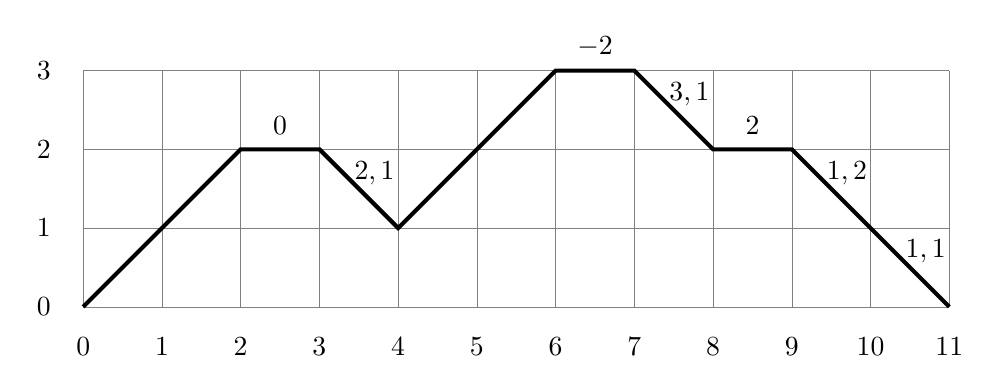
\begin{tikzpicture}
\draw[help lines] (0,0) grid (11,3);
\foreach \x in {0,...,11} \draw node at (\x,-.5) {\( \x \)};
\foreach \y in {0,...,3} \draw node at (-.5,\y) {\( \y \)};
\draw[line width = 1.5pt] (0,0) -- ++(1,1) -- ++(1,1) -- ++(1,0) -- ++(1,-1) -- ++(1,1) -- ++(1,1) -- ++(1,0) -- ++(1,-1) -- ++(1,0) -- ++(1,-1) -- ++(1,-1);
\node at (2.5,2.3) {\( 0 \)};
\node at (3.7,1.7) {\( 2,1 \)};
\node at (6.5,3.3) {\( -2 \)};
\node at (7.7,2.7) {\( 3,1 \)};
\node at (8.5,2.3) {\( 2 \)};
\node at (9.7,1.7) {\( 1,2 \)};
\node at (10.7,.7) {\( 1,1 \)};
\end{tikzpicture}

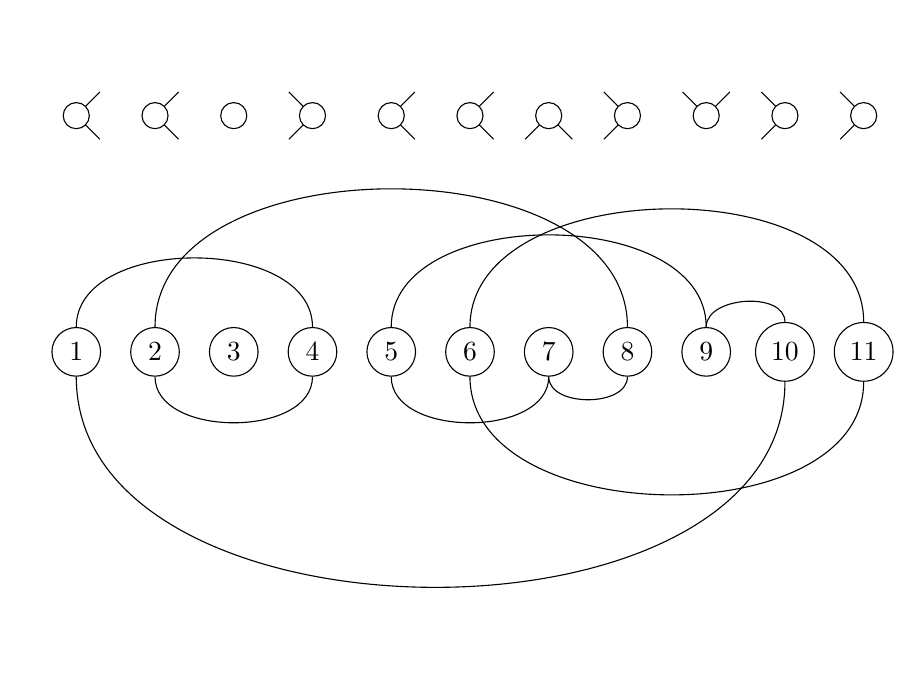
\begin{tikzpicture}
\begin{scope}[shift={(0,0)}]
\node (0,0) at (0.5,1) {};
\draw (1.3,-.3) -- (1,0) -- (1.3,0.3);
\draw (2.3,-0.3) -- (2,0) -- (2.3,0.3);
\draw (3.7,-0.3) -- (4,0) -- (3.7,0.3);
\draw (5.3,-0.3) -- (5,0) -- (5.3,0.3);
\draw (6.3,-0.3) -- (6,0) -- (6.3,0.3);
\draw (6.7,-0.3) -- (7,0) -- (7.3,-0.3);
\draw (7.7,-0.3) -- (8,0) -- (7.7,0.3);
\draw (8.7,0.3) -- (9,0) -- (9.3,0.3);
\draw (9.7,-0.3) -- (10,0) -- (9.7,0.3);
\draw (10.7,-0.3) -- (11,0) -- (10.7,0.3);
\node[draw,circle,fill=white] (1) at (1,0) {};
\node[draw,circle,fill=white] (4) at (4,0) {};
\node[draw,circle,fill=white] (2) at (2,0) {};
\node[draw,circle,fill=white] (7) at (7,0) {};
\node[draw,circle,fill=white] (3) at (3,0) {};
\node[draw,circle,fill=white] (5) at (5,0) {};
\node[draw,circle,fill=white] (6) at (6,0) {};
\node[draw,circle,fill=white] (8) at (8,0) {};
\node[draw,circle,fill=white] (9) at (9,0) {};
\node[draw,circle,fill=white] (10) at (10,0) {};
\node[draw,circle,fill=white] (11) at (11,0) {};
\end{scope}
\begin{scope}[shift={(0,-3)}]
\node[draw, circle] (1) at (1,0) {\( 1 \)};
\node[draw, circle] (4) at (4,0) {\( 4 \)};
\node[draw, circle] (6) at (6,0) {\( 6 \)};
\node[draw, circle] (2) at (2,0) {\( 2 \)};
\node[draw, circle] (3) at (3,0) {\( 3 \)};
\node[draw, circle] (5) at (5,0) {\( 5 \)};
\node[draw, circle] (7) at (7,0) {\( 7 \)};
\node[draw, circle] (8) at (8,0) {\( 8 \)};
\node[draw, circle] (9) at (9,0) {\( 9 \)};
\node[draw, circle] (10) at (10,0) {\( 10 \)};
\node[draw, circle] (11) at (11,0) {\( 11 \)};
\draw[out=90,in=90] (1) to (4);
\draw[out=90,in=90] (2) to (8);
\draw[out=90,in=90] (5) to (9);
\draw[out=90,in=90] (6) to (11);
\draw[out=90,in=90] (9) to (10);
\draw[out=-90,in=-90] (4) to (2);
\draw[out=-90,in=-90] (5) to (7);
\draw[out=-90,in=-90] (7) to (8);
\draw[out=-90,in=-90] (1) to (10);
\draw[out=-90,in=-90] (6) to (11);
\end{scope}
\end{tikzpicture}
\caption{A modified Laguerre history in \( \LH_{11} \) and the
  corresponding diagram representing a permutation.}
  \label{fig:Lag-his-modified}
\end{figure}

It is not hard to show that the above map \( \rho\mapsto \pi \) is a
bijection from the set of modified Laguerre histories of length
\( n \) to \( \sym_n \). Moreover, this map has the property
\( \max(\rho) = \LRmax(\pi) \), where \( \max(\rho) \) is the number
of maximum possible labels of a horizontal step plus the number of
maximum possible labels in the first component of a down step and
\( \LRmax(\pi) \) is the number of left-to-right maxima of
\( \pi=\pi_1 \cdots \pi_n \), that is \( \pi_i \) such that
\( \pi_i = \max\{\pi_1,\dots,\pi_i\} \).
This implies that
\[
  \mu_n = \sum_{\pi\in \sym_n} \alpha^{\LRmax(\pi)}.
\]

For example, suppose \( \rho \) and \( \pi \) are as in
\Cref{fig:Lag-his-modified}. Then the \( i \)th step is a horizontal
step with maximum possible label or a down step with maximum possible
lable in the first component for \( i=4,8,9,11 \). The left-to-right
maxima of \( \pi \) are exactly \( 4,8,9,11 \).



\chapter{Duality between mixed moments and coefficients}

Suppose that \( \{ P_n(x) \}_{n\ge 0} \) is a monic
OPS given by
\[
    P_n(x) = \sum_{k=0}^{n} \nu_{n,k} x^k.
\]
In this chapter we will show that
\[
  x^n = \sum_{k=0}^{n} \mu_{n,k} P_k(x),
\]
where \( \mu_{n,k} = \LL(x^nP_k(x))/\LL(P_k(x)^2) \) is the mixed
moment. We then show the duality between the mixed moments
\( \mu_{n,k} \) and the coefficients \( \nu_{n,k} \) combinatorially.
As special cases we obtain
various known dualities among
binomial coefficients,
\( q \)-binomial coefficients,
Stirling numbers, and
elementary and homogeneous symmetric functions.



\section{Mixed moments and coefficients}



As before suppose that \( \{ P_n(x) \}_{n\ge 0} \) is a monic OPS with
a linear functional \( \LL \) given by
\[
  P_{n+1}(x) = (x-b_n) P_n(x) - \lambda_n P_{n-1}(x).
\]

Recall from \Cref{def:mixed_moment} and \Cref{thm:mu=Mot_nrs} that the
mixed moment \( \mu_{n,k} \) has the following
combinatorial interpretation:
\[
  \mu_{n,k} = \frac{\LL(x^nP_k(x))}{\LL(P_k(x))} = 
  \sum_{\pi\in \Motz_{n,k}} \wt(\pi).
\]
where \( \Motz_{n,k} \) is the set of Motzkin paths from \( (0,0) \)
to \( (n,k) \).


\begin{prop}\label{pro:1}
  We have
 \[
     x^n = \sum_{k=0}^{n} \mu_{n,k} P_k(x).
 \] 
\end{prop}

\begin{proof}
  Let
  \[
      x^n = \sum_{k=0}^{n} \sigma_{n,k} P_k(x).
  \]
  Multiplying \( P_k(x) \) and taking \( \LL \) both sides, we obtain
\[
  \LL(x^nP_k(x)) = \sigma_{n,k} \LL(P_k(x)^2).
\]
Hence
\[
  \sigma_{n,k} =  \frac{\LL(x^nP_k(x))}{\LL(P_k(x)^2)}
  = \mu_{n,k},
\]
as desired.
\end{proof}

Now let \( \nu_{n,k} \) be the coefficient of \( x^k \) in
\( P_n(x) \) so that
\begin{align*}
  x^n &= \sum_{k=0}^{n} \mu_{n,k} P_k(x),\\
  P_n(x) &= \sum_{k=0}^{n} \nu_{n,k} x^k.
\end{align*}
Since \( \{ P_n(x) \}_{n\ge 0} \) and \( \{x^n\}_{n\ge0} \) are bases
of the space of polynomials, we have the following matrix identities:
\[
  \left( \nu_{n,k} \right)_{n,k\ge0} \left( \mu_{n,k} \right)_{n,k\ge0} = 
  \left( \mu_{n,k} \right)_{n,k\ge0} \left( \nu_{n,k} \right)_{n,k\ge0} = I.
\]
Equivalently,
\begin{align}
  \label{eq:27}
\sum_{k\ge0} \nu_{n,k}\mu_{k,m} &= \delta_{n,m},\\
  \label{eq:28}
\sum_{k\ge0} \mu_{n,k}\nu_{k,m} &= \delta_{n,m}.
\end{align}


Since we have combinatorial interpretations for \( \mu_{n,k} \) and
\( \nu_{n,k} \), we can prove the above matrix identities
combinatorially. In fact, in the next section we will prove these
combinatorially without the assumption that \( \lambda_k\ne 0 \).

\section{Combinatorial proof of duality}

Suppose that \( \{b_n\}_{n\ge0} \) and \( \{\lambda_n\}_{n\ge1} \) are
arbitrary sequences (\( \lambda_n \) may be zero). Then we can take
the following as definitions:
\begin{align*}
  \mu_{n,k} &= \sum_{\pi\in \Motz_{n,k}} \wt(\pi),\\
  \nu_{n,k} &= \sum_{T\in \FT_{n,k}} \wt'(T),
\end{align*}
where \( \FT_{n,k} \) is the set of Favard tilings in \( \FT_n \) with
\( k \) red monominos, see \Cref{fig:2}. Observe that
\( \mu_{n,k} = \nu_{n,k}=0 \) if 
\( n<k \).

\begin{figure}
  \centering
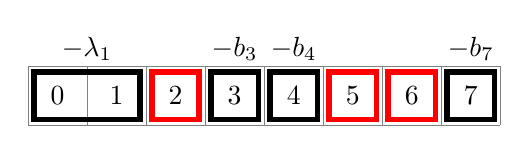
\begin{tikzpicture}[scale=0.75]
  \draw [help lines] (0,0) grid (8,1);
  \foreach \x in {0,...,7} \draw node at (\x+.5,.5) {\x};
  \LBD1 \RM2 \LBM3 \LBM4 \RM5 \RM6 \LBM7
\end{tikzpicture}
\caption{A Favard tiling $T\in\FT_{8,3}$ with
  $\wt'(T)=\lambda_1 b_3b_4b_7$.}
\label{fig:2}
\end{figure}


The following theorem can be proved similarly to the proof of
\Cref{thm:5}. We give a proof of this theorem to compare it with that
of the next theorem.

\begin{thm}\label{thm:1}
  For nonnegative integers \( n \) and \( m \), we have
  \[
    \sum_{k\ge0} \nu_{n,k}\mu_{k,m} = \delta_{n,m}.
  \]
\end{thm}

\begin{proof}
  Since the proof is similar to that of \Cref{thm:5}, we only
  give a sketch. Note that the sum in the theorem is \( 0 \) if
  \( n<m \) because \( \nu_{n,k}\mu_{k,m}=0 \) unless
  \( n\ge k\ge m \). Thus we may assume \( n\ge m \).

  Let \( X \) be the set of pairs \( (T,\pi) \) of a Favard tiling
  \( T\in \FT_{n,k} \) and a Motzkin path \( \pi\in \Motz_{k,m} \),
  for some \( m\le k\le n \). Let \( Y \) be the set of pairs
  \( (T,\pi) \) of a Favard tiling \( T\in \FT_{n,n} \) and a Motzkin
  path \( \pi\in \Motz_{n,m} \) such that \( T \) has red monominos
  only and \( \pi \) has up steps only. Then \( Y \) has a unique
  element if \( n=m \); and \( Y=\emptyset \) if \( n\ne m \).

  Our goal is to find a weight-preserving sign-reversing involution
  \( \phi: X \to X \) with fixed point set \( Y \). To do this, let
  \( (T,\pi)\in X \) with \( T\in \FT_{n,k} \) and
  \( \pi\in \Motz_{k,m} \). We write \( \pi=S_1S_2 \cdots S_{k} \) as
  a sequence of steps. Let \( a,u \) be the integers defined as
  follows:
 \begin{itemize}
 \item \( a \) is the largest integer such that \( T \)
   starts with \( a \) red monominos,
 \item \( u \) is the largest integer such that \( \pi \) starts with
   \( u \) up steps.
 \end{itemize}
 We define \( \phi(T,\pi)= (T',\pi') \) in the following way. Here,
 \( a',u' \) are the integers defined similarly as above using
 \( T' \) and \( \pi' \).
\begin{description}
\item[Case 1] \( u<a \). There are two
  subcases.
\begin{description}
\item[Case 1-1] \( S_{u+1} \) is a horizontal step. Let
  \[
    \pi' = S_1\cdots \widehat{S_{u+1}} \cdots S_{k},
  \]
and define $T'$ to be the Favard tiling obtained from $T$ by replacing
the \( (u+1) \)st red monomino by a black monomino. See
Figure~\ref{fig:1}.
\item[Case 1-2] $S_{u+1}$ is a down step. Let
  \[
    \pi' = S_1\cdots \widehat{S_{u}}\widehat{S_{u+1}} \cdots S_k,
  \]
and define $T'$ to be the Favard tiling obtained from $T$ by replacing
the \( u \)th and \( (u+1) \)st red monominos by a domino. See
Figure~\ref{fig:3}.
\end{description}

\item[Case 2] \( u\ge a\ne n \). Let \( A \) be the \( (a+1) \)st tile
  in \( T \). There are two subcases.
  \begin{description}
  \item[Case 2-1] $A$ is a black monomino. In this case let
    \[
      \pi' = S_1\cdots S_a H S_{a+1} \cdots S_k,
    \]
and define $T'$ to be the Favard tiling obtained from $T$ by
replacing $A$ by a red monomino. See Figure~\ref{fig:1} (with the
roles of \( (T,\pi) \) and \( (T',\pi') \) interchanged).
\item[Case 2-2] $A$ is a domino. In this case let
  \[
    \pi' = S_1\dots S_a UD S_{a+1} \dots S_k,
  \]
and define $T'$ to be the Favard tiling obtained from $T$ by
replacing $A$ by two red monominos. See Figure~\ref{fig:3} (with
the roles of \( (T,\pi) \) and \( (T',\pi') \)
interchanged).
\end{description}
\item[Case 3] \( u\ge a = n \). Since \( u\le k\le n \), we must have \( u=a=n \).
  Then \( T \) has only red monominos and \( \pi \) has only up steps.
  We define \( (T',\pi') = (T,\pi) \).
\end{description}

The map \( \phi:X \to X \) is a weight-preserving sign-reversing
involution with fixed point set \( Y \). Hence
\[
  \sum_{(T,\pi)\in X} \wt'(T) \wt(\pi) = \sum_{(T,\pi)\in Y} \wt'(T)
  \wt(\pi) = \delta_{n,m}.
\]
\end{proof}



\begin{figure}
  \centering
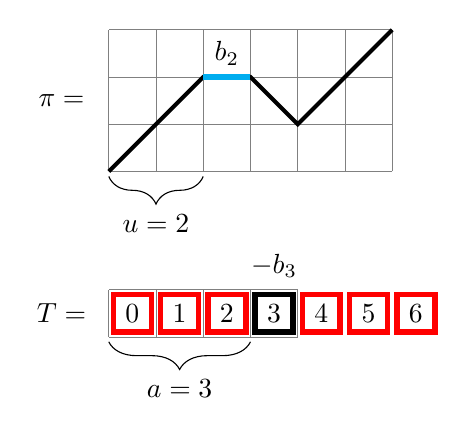
\begin{tikzpicture}[scale=0.6]
  \draw[help lines] (0,0) grid (6,3);
\draw[line width = 1.5pt] (0,0) -- ++(1,1) -- ++(1,1) -- ++(1,0) -- ++(1,-1) -- ++(1,1) -- ++(1,1);
  \draw [decorate,decoration={brace,amplitude=10pt},xshift=-0pt,yshift=-3pt]
(2,0) -- (0,0) node [black,midway,yshift=-0.6cm] {\( u=2 \)};
\node at (-1,1.5) {\( \pi= \)};
\node at (2.5,2.5) {\( b_2 \)};
\draw[line width = 2pt, cyan] (2,2)--++(1,0);
\begin{scope}[shift={(0,-3.5)}]
  \draw [help lines] (0,0) grid (4,1);
  \foreach \x in {0,...,6} \draw node at (\x+0.5,0.5) {\x};
  \RM0 \RM1 \RM2 \BM3 \RM4 \RM5 \RM6 
  \node at (3.5,1.5) {\( -b_3 \)};
  \draw [decorate,decoration={brace,amplitude=10pt},xshift=-0pt,yshift=-3pt]
(3,0) -- (0,0) node [black,midway,yshift=-0.6cm] {\( a=3 \)};
\node at (-1,.5) {\( T= \)};
\end{scope}
\end{tikzpicture} \quad
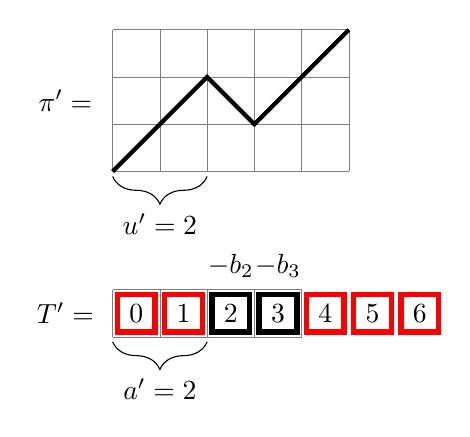
\begin{tikzpicture}[scale=0.6]
  \draw[help lines] (0,0) grid (5,3);
\draw[line width = 1.5pt] (0,0) -- ++(1,1) -- ++(1,1) -- ++(1,-1) -- ++(1,1) -- ++(1,1);
  \draw [decorate,decoration={brace,amplitude=10pt},xshift=-0pt,yshift=-3pt]
(2,0) -- (0,0) node [black,midway,yshift=-0.6cm] {\( u'=2 \)};
\node at (-1,1.5) {\( \pi'= \)};
\remove(2,2)
\begin{scope}[shift={(0,-3.5)}]
  \draw [help lines] (0,0) grid (4,1);
  \foreach \x in {0,...,6} \draw node at (\x+0.5,0.5) {\x};
  \RM0 \RM1 \BM2 \BM3 \RM4 \RM5 \RM6
  \draw [decorate,decoration={brace,amplitude=10pt},xshift=-0pt,yshift=-3pt]
(2,0) -- (0,0) node [black,midway,yshift=-0.6cm] {\( a'=2 \)};
\node at (-1,.5) {\( T'= \)};
  \node at (2.5,1.5) {\( -b_2 \)};
  \node at (3.5,1.5) {\( -b_3 \)};
\end{scope}
\end{tikzpicture}  
\caption{A pair \( (T,\pi)\in X \) in Case 1-1 on the left and the
  corresponding triple \( (T',\pi')\in X \) in Case 2-1 on the right.}
\label{fig:1}
\end{figure}

\begin{figure}
  \centering
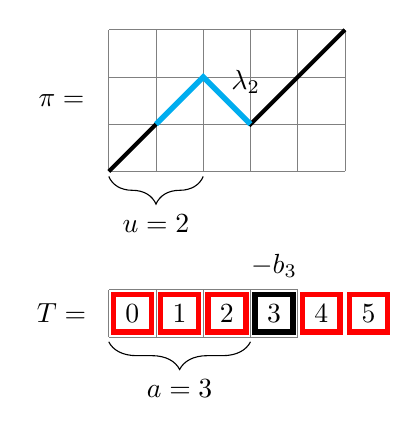
\begin{tikzpicture}[scale=0.6]
  \draw[help lines] (0,0) grid (5,3);
\draw[line width = 1.5pt] (0,0) -- ++(1,1) -- ++(1,1) -- ++(1,-1) -- ++(1,1) -- ++(1,1);
  \draw [decorate,decoration={brace,amplitude=10pt},xshift=-0pt,yshift=-3pt]
(2,0) -- (0,0) node [black,midway,yshift=-0.6cm] {\( u=2 \)};
\node at (-1,1.5) {\( \pi= \)};
\node at (2.9,1.9) {\( \lambda_2 \)};
\draw[line width = 2pt, cyan] (1,1) -- (2,2)--++(1,-1);
\begin{scope}[shift={(0,-3.5)}]
  \draw [help lines] (0,0) grid (4,1);
  \foreach \x in {0,...,5} \draw node at (\x+0.5,0.5) {\x};
  \RM0 \RM1 \RM2 \BM3 \RM4 \RM5
  \draw [decorate,decoration={brace,amplitude=10pt},xshift=-0pt,yshift=-3pt]
(3,0) -- (0,0) node [black,midway,yshift=-0.6cm] {\( a=3 \)};
\node at (-1,.5) {\( T= \)};
\node at (3.5,1.5) {\( -b_3 \)};
\end{scope}
\end{tikzpicture} \quad
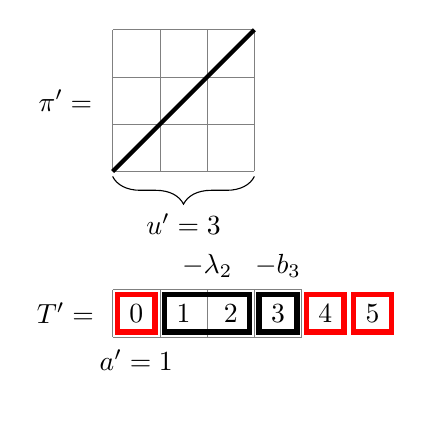
\begin{tikzpicture}[scale=0.6]
  \draw[help lines] (0,0) grid (3,3);
\draw[line width = 1.5pt] (0,0) -- ++(1,1) -- ++(1,1) -- ++(1,1);
  \draw [decorate,decoration={brace,amplitude=10pt},xshift=-0pt,yshift=-3pt]
(3,0) -- (0,0) node [black,midway,yshift=-0.6cm] {\( u'=3 \)};
\node at (-1,1.5) {\( \pi'= \)};
\remove(1,1)
\begin{scope}[shift={(0,-3.5)}]
  \draw [help lines] (0,0) grid (4,1);
  \foreach \x in {0,...,5} \draw node at (\x+0.5,0.5) {\x};
  \RM0 \BD2 \BM3 \RM4 \RM5
\node at (-1,.5) {\( T'= \)};
\node at (.5,-.5) {\( a'=1 \)};
\node at (3.5,1.5) {\( -b_3 \)};
\node at (2,1.5) {\( -\lambda_2 \)};
  \phantom{\draw [decorate,decoration={brace,amplitude=10pt},xshift=-0pt,yshift=-3pt]
(3,0) -- (0,0) node [black,midway,yshift=-0.6cm] {\( a=3 \)};}
\end{scope}
\end{tikzpicture}  
\caption{A pair \( (T,\pi)\in X \) in Case 1-2 on the left and the
  corresponding triple \( (T',\pi')\in X \) in Case 2-2 on the right.}
\label{fig:3}
\end{figure}

Now we prove the other duality.

\begin{thm}\label{thm:2}
  For nonnegative integers \( n \) and \( m \), we have
  \[
    \sum_{k\ge0} \mu_{n,k}\nu_{k,m} = \delta_{n,m}.
  \]
\end{thm}

\begin{proof}
  The proof is quite similar to that of \Cref{thm:1} except that we
  consider the end of a Motzkin instead of its beginning. Again, we
  may assume \( n\ge m \).

  Let \( X \) be the set of pairs \( (\pi,T) \) of a Motzkin path
  \( \pi\in \Motz_{n,k} \) and a Favard tiling \( T\in \FT_{k,m} \),
  for some \( m\le k\le n \). Let \( Y \) be the set of pairs
  \( (\pi,T) \) of a Motzkin path \( \pi\in \Motz_{n,m} \) and a
  Favard tiling \( T\in \FT_{m,m} \) such that \( \pi \) has up steps
  only and \( T \) has red monominos only. Then \( Y \) has a unique
  element if \( n=m \); and \( Y=\emptyset \) if \( n\ne m \).

  Our goal is to find a weight-preserving sign-reversing involution
  \( \phi: X \to X \) with fixed point set \( Y \). To do this, let
  \( (\pi,T)\in X \) with \( \pi\in \Motz_{n,k} \) and
  \( T\in \FT_{k,m} \) with \( m\le k\le n \). We write
  \( \pi=S_nS_{n-1} \cdots S_{1} \) as a sequence of steps. Let
  \( a,u \) be the integers defined as follows:
 \begin{itemize}
 \item \( a \) is the largest integer such that \( T \)
   end with \( a \) red monominos,
 \item \( u \) is the largest integer such that \( \pi \) ends with
   \( u \) up steps.
 \end{itemize}
 We define \( \phi(\pi,T)= (\pi',T') \) in the following way. Here,
 \( a',u' \) are the integers defined similarly as above using
 \( \pi' \) and \( T' \).
\begin{description}
\item[Case 1] \( n\ne u\le a \). There are two
  subcases.
\begin{description}
\item[Case 1-1] \( S_{u+1} \) is a horizontal step. Let \( \pi' \) be
  the Motzkin path obtained from \( \pi \) by replacing \( S_{u+1} \)
  by \( U \) and define $T'$ to be the Favard tiling obtained from $T$
  by inserting a black monomino before the last \( u \) red monominos.
  See Figure~\ref{fig:4}.
\item[Case 1-2] $S_{u+1}$ is a down step. Let \( \pi' \) be
  the Motzkin path obtained from \( \pi \) by replacing \( S_{u+1} \)
  by \( U \) and define $T'$ to be the Favard tiling obtained from $T$
  by inserting a black domino before the last \( u \) red monominos.
 See Figure~\ref{fig:5}.
\end{description}

\item[Case 2] \( u> a \). Since \( a<u\le k \), we can let \( A \) be
  the \( (a+1) \)st tile from the right in \( T \). There are two
  subcases.
  \begin{description}
  \item[Case 2-1] $A$ is a black monomino. Let \( \pi' \) be the
    Motzkin path obtained from \( \pi \) by replacing \( S_{a+1} \) by
    \( H \) and define $T'$ to be the Favard tiling obtained from $T$
    by deleting the \( (a+1) \)st tile from the right in \( T \). See
    Figure~\ref{fig:4}. (with the roles of \( (\pi,T) \) and
    \( (\pi',T') \) interchanged).
\item[Case 2-2] $A$ is a domino. Let \( \pi' \) be the
    Motzkin path obtained from \( \pi \) by replacing \( S_{a+1} \) by
    \( D \) and define $T'$ to be the Favard tiling obtained from $T$
    by deleting the \( (a+1) \)st tile from the right in \( T \). See
    Figure~\ref{fig:5}. (with the roles of \( (\pi,T) \) and
    \( (\pi',T') \) interchanged).
\end{description}
\item[Case 3] \( n = u\le a \). Since \( n\ge m \ge a \), we must have
  \( u=a=n \). Then \( T \) has only red monominos and \( \pi \) has
  only up steps. We define \( (\pi',T') = (\pi,T) \).
\end{description}


The map \( \phi:X \to X \) is a weight-preserving sign-reversing
involution with fixed point set \( Y \). Hence
\[
  \sum_{(\pi,T)\in X} \wt'(T) \wt(\pi)
  =  \sum_{(\pi,T)\in Y}\wt'(T) \wt(\pi) = \delta_{n,m}.
\]
\end{proof}


\begin{figure}
  \centering
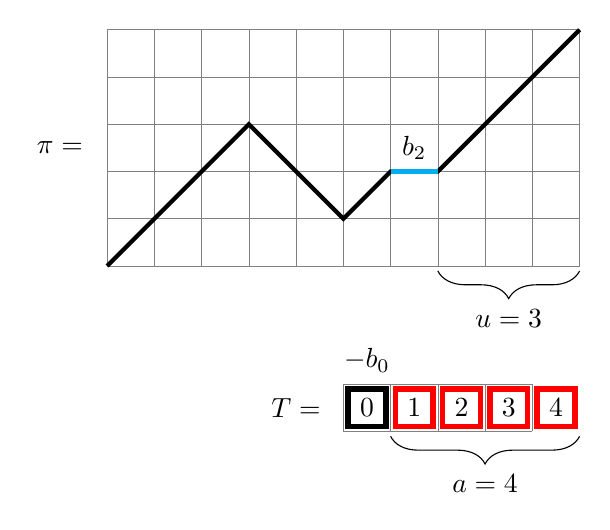
\begin{tikzpicture}[scale=0.6]
  \draw[help lines] (0,0) grid (10,5);
\draw[line width = 1.5pt] (0,0) -- ++(1,1) -- ++(1,1) -- ++(1,1) -- ++(1,-1) -- ++(1,-1) -- ++(1,1) -- ++(1,0) -- ++(1,1) -- ++(1,1) -- ++(1,1);
  \draw [decorate,decoration={brace,amplitude=10pt},xshift=-0pt,yshift=-3pt]
(10,0) -- (7,0) node [black,midway,yshift=-0.6cm] {\( u=3 \)};
\node at (-1,2.5) {\( \pi= \)};
\node at (6.5,2.5) {\( b_2 \)};
\draw[line width = 2pt, cyan] (6,2)--++(1,0);
\begin{scope}[shift={(5,-3.5)}]
  \draw [help lines] (0,0) grid (4,1);
  \foreach \x in {0,...,4} \draw node at (\x+0.5,0.5) {\x};
  \BM0 \RM1 \RM2 \RM3 \RM4
  \node at (0.5,1.5) {\( -b_0 \)};
  \draw [decorate,decoration={brace,amplitude=10pt},xshift=-0pt,yshift=-3pt]
(5,0) -- (1,0) node [black,midway,yshift=-0.6cm] {\( a=4 \)};
\node at (-1,.5) {\( T= \)};
\end{scope}
\end{tikzpicture} \quad
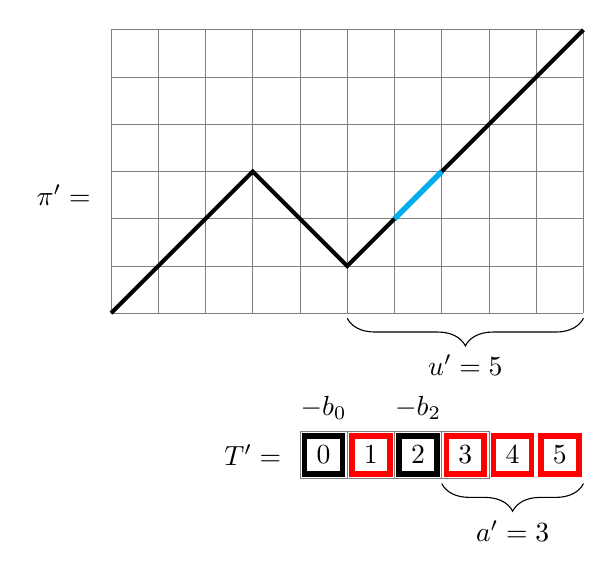
\begin{tikzpicture}[scale=0.6]
  \draw[help lines] (0,0) grid (10,6);
\draw[line width = 1.5pt] (0,0) -- ++(1,1) -- ++(1,1) -- ++(1,1) -- ++(1,-1) -- ++(1,-1) -- ++(1,1) -- ++(1,1) -- ++(1,1) -- ++(1,1) -- ++(1,1);
  \draw [decorate,decoration={brace,amplitude=10pt},xshift=-0pt,yshift=-3pt]
(10,0) -- (5,0) node [black,midway,yshift=-0.6cm] {\( u'=5 \)};
\node at (-1,2.5) {\( \pi'= \)};
\draw[line width = 2pt, cyan] (6,2)--++(1,1);
\begin{scope}[shift={(4,-3.5)}]
  \draw [help lines] (0,0) grid (4,1);
  \foreach \x in {0,...,5} \draw node at (\x+0.5,0.5) {\x};
  \BM0 \RM1 \BM2 \RM3 \RM4 \RM5
  \node at (0.5,1.5) {\( -b_0 \)};
  \node at (2.5,1.5) {\( -b_2 \)};
  \draw [decorate,decoration={brace,amplitude=10pt},xshift=-0pt,yshift=-3pt]
(6,0) -- (3,0) node [black,midway,yshift=-0.6cm] {\( a'=3 \)};
\node at (-1,.5) {\( T'= \)};
\end{scope}
\end{tikzpicture}  
\caption{A pair \( (T,\pi)\in X \) in Case 1-1 on the left and the
  corresponding triple \( (T',\pi')\in X \) in Case 2-1 on the right.}
\label{fig:4}
\end{figure}

\begin{figure}
  \centering
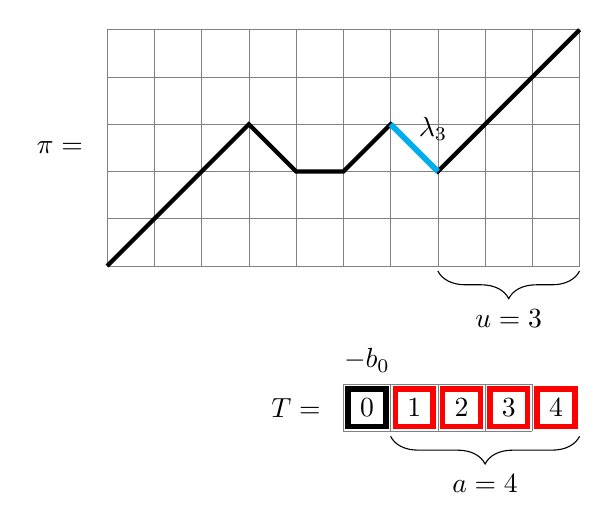
\begin{tikzpicture}[scale=0.6]
  \draw[help lines] (0,0) grid (10,5);
\draw[line width = 1.5pt] (0,0) -- ++(1,1) -- ++(1,1) -- ++(1,1) -- ++(1,-1) -- ++(1,0) -- ++(1,1) -- ++(1,-1) -- ++(1,1) -- ++(1,1) -- ++(1,1);
  \draw [decorate,decoration={brace,amplitude=10pt},xshift=-0pt,yshift=-3pt]
(10,0) -- (7,0) node [black,midway,yshift=-0.6cm] {\( u=3 \)};
\node at (-1,2.5) {\( \pi= \)};
\node at (6.9,2.9) {\( \lambda_3 \)};
\draw[line width = 2pt, cyan] (6,3)--++(1,-1);
\begin{scope}[shift={(5,-3.5)}]
  \draw [help lines] (0,0) grid (4,1);
  \foreach \x in {0,...,4} \draw node at (\x+0.5,0.5) {\x};
  \BM0 \RM1 \RM2 \RM3 \RM4
  \node at (0.5,1.5) {\( -b_0 \)};
  \draw [decorate,decoration={brace,amplitude=10pt},xshift=-0pt,yshift=-3pt]
(5,0) -- (1,0) node [black,midway,yshift=-0.6cm] {\( a=4 \)};
\node at (-1,.5) {\( T= \)};
\end{scope}
\end{tikzpicture} \quad
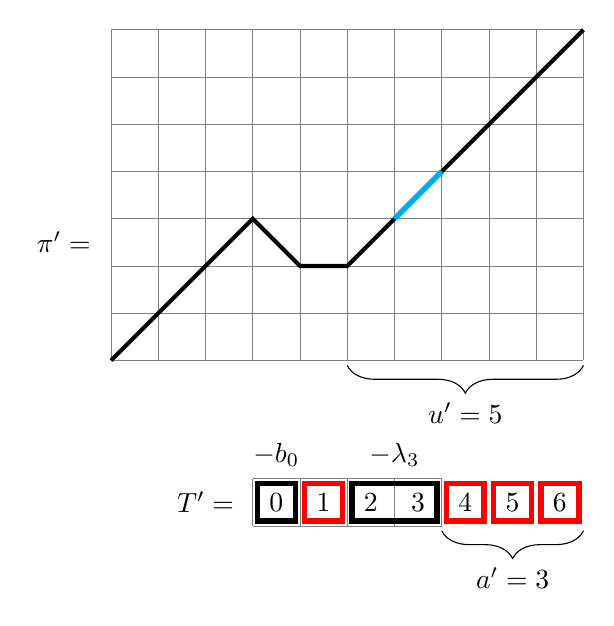
\begin{tikzpicture}[scale=0.6]
  \draw[help lines] (0,0) grid (10,7);
\draw[line width = 1.5pt] (0,0) -- ++(1,1) -- ++(1,1) -- ++(1,1) -- ++(1,-1) -- ++(1,0) -- ++(1,1) -- ++(1,1) -- ++(1,1) -- ++(1,1) -- ++(1,1);
  \draw [decorate,decoration={brace,amplitude=10pt},xshift=-0pt,yshift=-3pt]
(10,0) -- (5,0) node [black,midway,yshift=-0.6cm] {\( u'=5 \)};
\node at (-1,2.5) {\( \pi'= \)};
\draw[line width = 2pt, cyan] (6,3)--++(1,1);
\begin{scope}[shift={(3,-3.5)}]
  \draw [help lines] (0,0) grid (4,1);
  \foreach \x in {0,...,6} \draw node at (\x+0.5,0.5) {\x};
  \BM0 \RM1 \BD3 \RM4 \RM5 \RM6
  \node at (0.5,1.5) {\( -b_0 \)};
  \node at (3,1.5) {\( -\lambda_3 \)};
  \draw [decorate,decoration={brace,amplitude=10pt},xshift=-0pt,yshift=-3pt]
(7,0) -- (4,0) node [black,midway,yshift=-0.6cm] {\( a'=3 \)};
\node at (-1,.5) {\( T'= \)};
\end{scope}
\end{tikzpicture}  
\caption{A pair \( (T,\pi)\in X \) in Case 1-2 on the left and the
  corresponding triple \( (T',\pi')\in X \) in Case 2-2 on the right.}
\label{fig:5}
\end{figure}


\section{Special case: elementary and homogeneous symmetric functions}

For the rest of this chapter we will study several special cases of
the duality between \( \mu_{n,k} \) and \( \nu_{n,k} \). In this
section we consider the case that \( b_k \) are arbitrary and
\( \lambda_k =0 \). The next sections will cover some interesting
special cases of this.

Suppose that \( b_k=x_{k} \) and \( \lambda_k =0 \), where \( x_0,x_1,\dots \) are
indeterminates. Observe that if \( \lambda_k=0 \), then
\( \pi\in \Motz_{n,k} \) is a path from \( (0,0)\to (n,k) \)
consisting of up steps \( U=(1,1) \) and horizontal steps
\( H=(1,0) \). By replacing each \( U=(1,1) \) by \( U'=(1,0) \), we
can identify \( \pi \) as a path from \( (0,0) \) to \( (n-k,k) \),
see \Cref{fig:6}.


\begin{figure}
  \centering
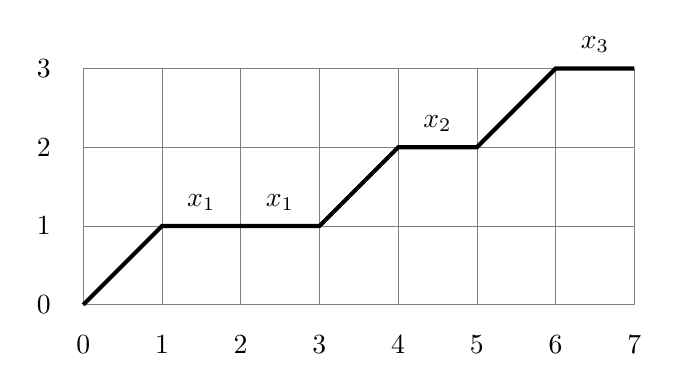
\begin{tikzpicture}
\draw[help lines] (0,0) grid (7,3);
\foreach \x in {0,...,7} \draw node at (\x,-.5) {\( \x \)};
\foreach \y in {0,...,3} \draw node at (-.5,\y) {\( \y \)};
\draw[line width = 1.5pt] (0,0) -- ++(1,1) -- ++(1,0) -- ++(1,0) -- ++(1,1) -- ++(1,0) -- ++(1,1) -- ++(1,0);
\hlabel11{x_1}
\hlabel21{x_1}
\hlabel42{x_2}
\hlabel63{x_3}
\end{tikzpicture} \qquad 
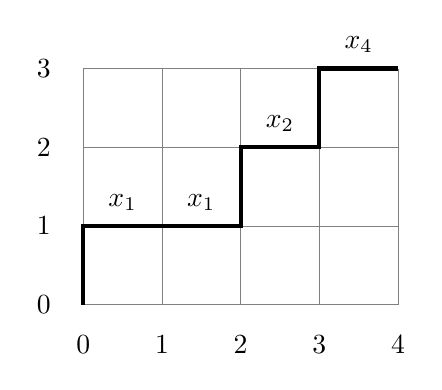
\begin{tikzpicture}
\draw[help lines] (0,0) grid (4,3);
\foreach \x in {0,...,4} \draw node at (\x,-.5) {\( \x \)};
\foreach \y in {0,...,3} \draw node at (-.5,\y) {\( \y \)};
\draw[line width = 1.5pt] (0,0) -- ++(0,1) -- ++(1,0) -- ++(1,0) -- ++(0,1) -- ++(1,0) -- ++(0,1) -- ++(1,0);
\hlabel01{x_1}
\hlabel11{x_1}
\hlabel22{x_2}
\hlabel33{x_4}
\end{tikzpicture}
\caption{A path with steps \( U=(1,1) \) and \( H=(1,0) \) on the left
  and the corresponding path with steps \( U'=(0,1) \) and
  \( H=(1,0) \) on the right.}
  \label{fig:6}
\end{figure}

Therefore we can write 
\[
  \mu_{n,k} = \sum_{\pi:(0,0)\to (n-k,k)} \wt(\pi),
\]
where the sum is over all paths \( \pi \) from \( (0,0) \) to
\( (n-k,k) \) with steps \( U' \) and \( H \), and \( \wt(\pi) \) is
the product of \( x_k \) for each horizontal step of height \( k \).
Such a path is completely determined by its weight. For example, the
path in \Cref{fig:6} is the unique path from \( (0,0) \) to
\( (4,3) \) with weight \( x_1^2 x_2 x_3 \).
Moreover, every weight is of the form \( x_{i_1}\cdots x_{i_{n-k}} \)
with \( 0\le i_1 \le \cdots \le i_{n-k} \le k \).
Thus
\begin{equation}\label{eq:29}
  \mu_{n,k} = \sum_{0\le i_1 \le \cdots \le i_{n-k} \le k} x_{i_1}\cdots x_{i_{n-k}}.
\end{equation}
This is a homogeneous symmetric polynomial.

\begin{defn}\label{def:1}
  Let \( x=(x_0,x_1,\dots) \) be a sequence of variables. A power
  series \( f(x_0,x_1,\dots) \) in the variables \( x \) is called a
  \emph{symmetric function} if it is invariant under permuting
  variables. A \emph{homogeneous symmetric function}
  \( h_k \) is defined by
  \[
    h_k = \sum_{i_1 \le \cdots \le i_{k}} x_{i_1}\cdots x_{i_{k}}.
  \]
  An \emph{elementary symmetric function}
  \( e_k \) is defined by
  \[
    e_k = \sum_{i_1 < \cdots < i_{k}} x_{i_1}\cdots x_{i_{k}}.
  \]
  We define \( h_0 = e_0 = 1 \) and \( h_k = e_k = 0 \) if \( k<0 \).
  A \emph{homogeneous symmetric polynomial} \( h_k(x_0,x_1,\dots,x_n) \) is
  defined by
  \[
    h_k(x_0,x_1,\dots,x_n) = \sum_{0\le i_1 \le \cdots \le i_{k} \le n}
    x_{i_1}\cdots x_{i_{k}}.
  \]
  An \emph{elementary symmetric polynomial} \( e_k(x_0,x_1,\dots,x_n) \)
  is defined by
  \[
    e_k(x_0,x_1,\dots,x_n) = \sum_{0\le i_1 < \cdots < i_{k} \le n}
    x_{i_1}\cdots x_{i_{k}}.
  \]
\end{defn}

For example,
\begin{align*}
  h_1(x_0,x_1,x_2) &= e_1(x_0,x_1,x_2) = x_0 + x_1 + x_2,\\
  h_2(x_0,x_1,x_2) &= x_0^2+x_1^2+x_2^2 + x_0x_1+x_0x_2+x_1x_2,\\
  e_2(x_0,x_1,x_2) &= x_0x_1+x_0x_2+x_1x_2,\\
  e_3(x_0,x_1,x_2) &= x_0x_1x_2.
\end{align*}

Then we can rewrite \eqref{eq:29} as follows.

\begin{thm}\label{thm:3}
  Suppose that \( b_k=x_{k} \) and \( \lambda_k =0 \).
  Then
  \[
    \mu_{n,k} = h_{n-k}(x_0,x_1,\dots,x_{k}).
  \]
\end{thm}

Now we consider
\[
  \nu_{n,k} = \sum_{T\in \FT_{n,k}} \wt'(T).
\]
Since \( \lambda_i=0 \), every \( T\in \FT_{n,k} \) has red monominos
and black monominos only. Hence, \( T \) is determined by choosing
\( n-k \) squares for black monominos in a \( 1\times n \) board.
Moreover, \( \wt'(T) \) is of the form
\( (-1)^{n-k} x_{i_1} \cdots x_{i_{n-k}} \) for some
\( 0\le i_1 < \cdots <i_{n-k} \le n-1 \), see \Cref{fig:7}.
\begin{figure}
  \centering
  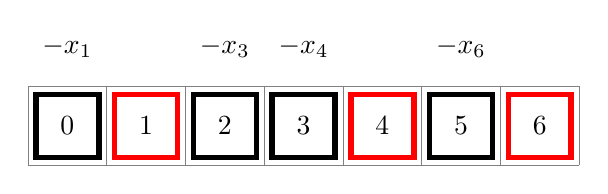
\begin{tikzpicture}
  \draw [help lines] (0,0) grid (7,1);
  \foreach \x in {0,...,6} \draw node at (\x+0.5,0.5) {\x};
  \BM0 \RM1 \BM2 \BM3 \RM4 \BM5 \RM6
  \node at (0.5,1.5) {\( -x_1 \)};
  \node at (2.5,1.5) {\( -x_3 \)};
  \node at (3.5,1.5) {\( -x_4 \)};
  \node at (5.5,1.5) {\( -x_6 \)};
  \end{tikzpicture}
  \caption{A Favard tiling with red monominos and black monominos.}
  \label{fig:7}
\end{figure}
This shows that
\[
    \nu_{n,k} = \sum_{0\le i_1 < \cdots <i_{n-k} \le n-1}(-1)^{n-k} x_{i_1} \cdots x_{i_{n-k}}.
\]
This can be restated as follows.

\begin{thm}\label{thm:4}
  Suppose that \( b_k=x_{k+1} \) and \( \lambda_k =0 \).
  Then
  \[
    \nu_{n,k} = (-1)^{n-k} e_{n-k}(x_0,x_1,\dots,x_{n-1}).
  \]
\end{thm}

By the duality (\Cref{thm:1} and \Cref{thm:2})
and \Cref{thm:3} and \Cref{thm:4},
we obtain the following corollary.

\begin{cor}\label{cor:1}
  The following matrix identities hold:
\begin{align*}
  \left( h_{n-k}(x_0,x_1,\dots,x_{k}) \right)_{n,k\ge0}
  \left( (-1)^{n-k} e_{n-k}(x_0,x_1,\dots,x_{n-1}) \right)_{n,k\ge0}
  &= I,\\
  \left( (-1)^{n-k} e_{n-k}(x_0,x_1,\dots,x_{n-1}) \right)_{n,k\ge0}
  \left( h_{n-k}(x_0,x_1,\dots,x_{k}) \right)_{n,k\ge0}
  &= I.
\end{align*}
Equivalently, for fixed integers \( n,m\ge0 \),
\begin{align}
\label{eq:31}  \sum_{k\ge 0} 
  h_{n-k}(x_0,x_1,\dots,x_{k}) (-1)^{k-m} e_{k-m}(x_0,x_1,\dots,x_{k-1}) 
  &= \delta_{n,m},\\
\label{eq:30}  \sum_{k\ge 0} (-1)^{n-k} e_{n-k}(x_0,x_1,\dots,x_{n-1}) h_{k-m}(x_0,x_1,\dots,x_{m})
  &= \delta_{n,m}.
\end{align}
\end{cor}

Suppose that \( N=n-m\ge0 \).
Then, by shifting the index \( k\mapsto k+m  \) in \eqref{eq:30}, we have
\[
  \sum_{k\ge 0} (-1)^{N-k} e_{N-k}(x_0,x_1,\dots,x_{m+N-1})
  h_{k}(x_0,x_1,\dots,x_{m}) = \delta_{N,0}.
\]
If we let \( m\to \infty \), we obtain
the well-known identity
\[
  \sum_{k\ge 0} (-1)^{k} e_{N-k} h_{k} = \delta_{N,0}.
\]

\section{Special case: binomial coefficients}

In this section we consider the case \( b_k=1 \) and
\( \lambda_k=0 \). We will show that the duality of this case is
related to the principle of inclusion and exclusion.

Suppose \( b_k=1 \) and \( \lambda_k=0 \). As observed in the previous
section, in this case \( \mu_{n,k} \) is the number of paths from
\( (0,0) \) to \( (n-k,k) \) using steps \( (1,0) \) and \( (0,1) \).
Thus \( \mu_{n,k} = \binom{n}{k} \). On the other hand,
\( \nu_{n,k} \) is \( (-1)^{n-k} \) times the number of Favard tilings
of size \( n \) with \( k \) red monominos and \( n-k \) black
monominos. Hence \( \nu_{n,k} = (-1)^{n-k}\binom{n}{k} \).

\begin{prop}
  If \( b_k=1 \) and \( \lambda_k=0 \), we have
\[
  \mu_{n,k} = \binom{n}{k}, \qquad 
  \nu_{n,k} = (-1)^{n-k} \binom{n}{k}.
\]
\end{prop}



As a corollary, we obtain the following duality between binomial
coefficients.

\begin{cor}\label{cor:2}
  We have
  \[
    \left( \binom{n}{k} \right)_{n,k\ge0}  \left( (-1)^{n-k} \binom{n}{k} \right)_{n,k\ge0}
    = 
    \left( (-1)^{n-k} \binom{n}{k} \right)_{n,k\ge0}
    \left( \binom{n}{k} \right)_{n,k\ge0}
    = I.
  \]
  Equivalently,
  \begin{equation}\label{eq:32}
  \left( \binom{n}{k} \right)_{n,k\ge0}^{-1} = 
  \left( (-1)^{n-k} \binom{n}{k} \right)_{n,k\ge0}.
\end{equation}
\end{cor}

Equation \eqref{eq:32} has an interesting connection with the
principle of inclusion and exclusion. To see this, suppose that
\( A_1,\dots,A_n \) are subsets of a set \( X \).
For a subset \( I \subseteq [n] \), we define
\begin{align*}
  A_{=I} &= \{ x\in X: x\in A_i \mbox{ if and only if \( i\in I \)}\},\\
  A_{\ge I} &= \{ x\in X: x\in A_i \mbox{ for all \( i\in I \)}\}.
\end{align*}
In other words, \( A_{=I} \) is the set of elements \( x \) which are
contained in exactly those \( A_i \) for \( i\in I \) and
\( A_{\ge I} \) is the set of elements \( x \) which are contained in
at least those \( A_i \) for \( i\in I \).

Note that 
\[
  A_{\ge I} = \bigcap_{i\in I} A_i = \bigcup_{J\supseteq I} A_{=J}.
\]
Thus
\begin{equation}\label{eq:33}
  \left| A_{\ge I} \right| = \sum_{J\supseteq I}  \left| A_{=J} \right|.
\end{equation}
We can invert this equation as follows, which is a form of the
principle of inclusion and exclusion.

\begin{lem}
  For any subset \( I \) of \( [n] \), we have
  \begin{equation}\label{eq:34}
  \left| A_{= I} \right| = \sum_{J\supseteq I} (-1)^{|J-I|}  \left| A_{\ge J} \right|.
\end{equation}
\end{lem}

\begin{proof}
  We will prove this by considering the contribution of each element
  \( x\in X \) to both sides of the equation. Note that every
  \( x\in X \) is contained in \( A_K \) for a unique subset \( K \)
  of \( [n] \). We consider the following three cases.

  \begin{description}
  \item[Case 1:] \( K=I \). Then the contribution of \( x \) in both sides is \( 1 \).
  \item[Case 2:] \( K \supsetneq I \). Then the contribution of
    \( x \) to the left-hand side is \( 0 \). The contribution of
    \( x \) to the right-hand side is
    \[
      \sum_{I \subseteq J \subseteq K} (-1)^{|J-I|} = 
      \sum_{J \subseteq (K-I)} (-1)^{|J|} = \sum_{j=0}^{|K-I|} (-1)^{j}\binom{|K-I|}{j} = 0.
    \]
  \item[Case 3:] \( K \not\supseteq I\). In this case the contribution
    of \( x \) in both sides is \( 0 \).
  \end{description}
  Since the contribution of \( x \) to both sides is always the same,
  the identity holds.
\end{proof}

If \( I=\emptyset \), we obtain the following common form of the principle
of inclusion and exclusion:
\begin{align*}
 \left| A_1^c  \cap \cdots \cap A_n^c \right| 
 &= \sum_{k=0}^{n} (-1)^{k} \sum_{i_1 < \cdots <i_k}
 \left| A_{i_1} \cap \cdots \cap A_{i_k} \right|\\
 &= |X| - |A_1| - \cdots - |A_n|\\
 & \qquad + |A_1\cap A_2| +|A_1\cap A_3| + \cdots + |A_{n-1}\cap A_{n}|\\
 & \qquad  - \cdots \\
 & \qquad + (-1)^{n}|A_1 \cap \cdots \cap A_n|.
\end{align*}


\begin{exam}
  A \emph{derangement} is a permutation without fixed points. Let
  \( d_n \) be the number of derangements in \( \sym_n \). To compute
  \( d_n \), we define \( X=\sym_n \) and
  \( A_i = \{\pi\in X: \pi(i) = i\} \).
  Then 
  \[
    d_n = |A_{=\emptyset}| = \sum_{J\subseteq[n]} (-1)^{|J|}|A_{\ge J}|.
  \]
  If \( J = \{j_1,\dots,j_k\} \), then \( |A_{\ge J}| = (n-k)! \).
  Thus
  \[
    d_n  = \sum_{k=0}^n  (-1)^{k} \binom{n}{k} (n-k)!
    = n! \sum_{k=0}^n  \frac{(-1)^{k}}{k!}.
  \]
  Note that
  \[
    \frac{d_n}{n!} = \sum_{k=0}^n  \frac{(-1)^{k}}{k!} \approx \frac{1}{e} = 0.367879441171\cdots.
  \]
\end{exam}

In the previous example, \( A_{=I} \) and \( A_{\ge I} \) depend only
on the cardinality of \( I \). In this case let \( a_k = |A_{=I}| \)
and \( b_k = |A_{\ge I}| \) for any subset \( I \) of cardinality
\( k \).
Then \eqref{eq:33} and \eqref{eq:34} can be written as
\begin{align*}
  b_k  &= \sum_{j=k}^n \binom{n-k}{j-k} a_j
         = \sum_{j=0}^{n-k} \binom{n-k}{j} a_{j+k},  \\
  a_k  &= \sum_{j=k}^n (-1)^{j-k}  \binom{n-k}{j-k} b_j
         = \sum_{j=0}^{n-k} (-1)^{j}  \binom{n-k}{j} b_{j+k}.
\end{align*}
To make things look nicer, let \( b'_k:= b_{n-k} \) and
\( a'_k:= a_{n-k} \).
Then the above equations can be rewritten as
\begin{align*}
  b'_{n-k}  &= \sum_{j=0}^{n-k} \binom{n-k}{n-k-j} a'_{n-k-j}
              = \sum_{j=0}^{n-k} \binom{n-k}{j} a'_{j},  \\
  a'_{n-k}  & = \sum_{j=0}^{n-k} (-1)^{j}  \binom{n-k}{n-k-j} b'_{n-k-j}
              = \sum_{j=0}^{n-k} (-1)^{n-k-j}  \binom{n-k}{j} b'_{j}.
\end{align*}
Finally, replacing \( k \) by \( n-k \), we obtain
\begin{align*}
  b'_{k}  & = \sum_{j=0}^{k} \binom{k}{j} a'_{j},  \\
  a'_{k}  & = \sum_{j=0}^{k} (-1)^{k-j}  \binom{k}{j} b'_{j}.
\end{align*}
Equivalently,
\begin{align*}
  \begin{pmatrix}
b'_0\\
\vdots\\
b'_n
\end{pmatrix}
&= \left( \binom{i}{j} \right)_{i,j=0}^n
\begin{pmatrix}
a'_0\\
\vdots\\
a'_n
\end{pmatrix}\\
  \begin{pmatrix}
a'_0\\
\vdots\\
a'_n
\end{pmatrix}
&= \left( (-1)^{i-j}\binom{i}{j} \right)_{i,j=0}^n
\begin{pmatrix}
b'_0\\
\vdots\\
b'_n
\end{pmatrix}
\end{align*}
Since \( a'_i \) and \( b'_i \) can be anything,
we have the following matrix identity:
\[
  \left( \binom{i}{j} \right)_{i,j=0}^n = 
  \left( (-1)^{i-j} \binom{i}{j} \right)_{i,j=0}^n,
\]
which is equivalent to \eqref{eq:32}.

\section{Special case: \( q \)-binomial coefficients}

In this section we consider the case \( b_k=q^k \) and
\( \lambda_k=0 \). This case gives \( q \)-binomial coefficients. We
first need some definitions. From now on, we treat \( q \) as an indeterminate.


\begin{defn}\label{def:2}
  For a nonnegative integer \( n \),
  the \emph{\( q \)-integer} \( [n]_q \) is defined by
  \[
    [n]_q = \frac{1-q^n}{1-q} = 1 + \cdots + q^{n-1}.
  \]
  The \emph{\( q \)-factorial} \( [n]_q! \) and the
  \emph{\( q \)-binomial coefficient} \( \qbinom{n}{k} \), for
  \( 0\le k\le n \), are defined by
  \[
    [n]_q! = [1]_q [2]_q \cdots [n]_q, \qquad
    \qbinom{n}{k} = \frac{[n]_q!}{[k]_q![n-k]_q!}.
  \]
  We also define \( \qbinom{n}{k} = 0 \) if \( n<k \).
\end{defn}


Note that if \( q=1 \), then
\[
  [n]_q = n, \qquad [n]_q! = n!, \qquad \qbinom{n}{k} = \binom{n}{k}.
\]

\begin{lem}\label{lem:2}
  For \( 0\le k\le n \), we have
  \begin{equation}\label{eq:35}
    \qbinom{n}{k} =  q^{n-k} \qbinom{n-1}{k-1} + \qbinom{n-1}{k}.
  \end{equation}
\end{lem}

\begin{proof}
  We compute
  \begin{align*}
    q^{n-k} \qbinom{n-1}{k-1} + \qbinom{n-1}{k}
    &= \frac{q^{n-k}[n-1]_q!}{[n-k]_q! [k-1]_q!}
    + \frac{[n-1]_q!}{[n-1-k]_q! [k]_q!},\\
    &= \frac{[n-1]_q!}{[n-k]_q! [k]_q!} \left( q^{n-k}[k]_q + [n-k]_q \right),\\
    &= \frac{[n-1]_q!}{[n-k]_q! [k]_q!} [n]_q = \qbinom{n}{k}. \qedhere
  \end{align*}
\end{proof}


\begin{defn}\label{def:3}
  A \emph{partition} is a sequence of nonnegative integers
  \( \lambda=(\lambda_1,\dots,\lambda_\ell) \) with
  \( \lambda_1 \ge \cdots \ge \lambda_\ell \). Each \( \lambda_i \) is
  called a \emph{part} of \( \lambda \). The \emph{size} of
  \( \lambda \) is defined to be
  \( |\lambda| = \lambda_1 + \cdots + \lambda_\ell \). The \emph{Young
    diagram} of \( \lambda \) is a left-justified array of squares
  where the \( i \)th row has \( \lambda_i \) squares.
  The \emph{transpose} \( \lambda' \) of \( \lambda \)
  is the partition whose Young diagram is obtained by reflecting
  the Young diagram of \( \lambda \) along the diagonal as shown in 
  \Cref{fig:8}.
\end{defn}

\begin{figure}
  \centering
\ydiagram{4,3,1} \qquad\qquad  \qquad 
\ydiagram{3,2,2,1}
\caption{The Young diagram of the partition \( \lambda=(4,3,1) \)
  and its transpose \( \lambda' = (3,2,2,1) \).}
  \label{fig:8}
\end{figure}

Let \( (a^b) \) denote the partition with \( b \) parts equal to
\( a \). For two partitions \( \lambda \) and \( \mu \), we write
\( \mu\subseteq\lambda \) to mean that the Young diagram of \( \mu \)
is contained in that of \( \lambda \). Note that considering the Young
diagram, \( \lambda\subseteq((n-k)^{k}) \) can be identified with a
path from \( (0,0) \) to \( (n-k,k) \), see \Cref{fig:9}. The
following proposition shows that the \( q \)-binomial coefficient
\( \qbinom{n}{k} \) is always a polynomial in \( q \).

\begin{figure}
  \centering
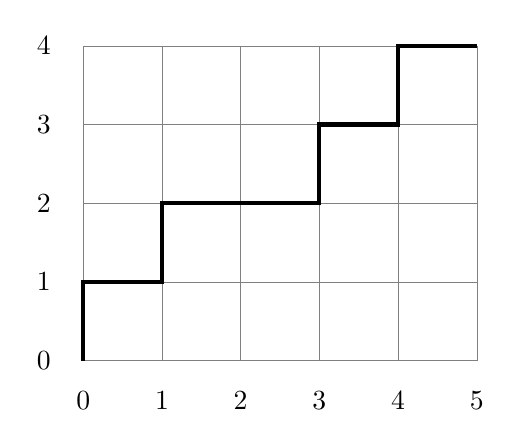
\begin{tikzpicture}
\draw[help lines] (0,0) grid (5,4);
\foreach \x in {0,...,5} \draw node at (\x,-.5) {\( \x \)};
\foreach \y in {0,...,4} \draw node at (-.5,\y) {\( \y \)};
\draw[line width = 1.5pt] (0,0) -- ++(0,1) -- ++(1,0) -- ++(0,1) -- ++(1,0) -- ++(1,0) -- ++(0,1) -- ++(1,0) -- ++(0,1) -- ++(1,0);
\end{tikzpicture}
\caption{The path corresponding to a partition \( \lambda=(4,3,1) \)
contained in a rectangle \( (5^4) \).}
  \label{fig:9}
\end{figure}


\begin{prop}
  For \( 0\le k\le n \), we have
\begin{equation}\label{eq:36}
  \qbinom{n}{k} = \sum_{\lambda\subseteq((n-k)^k)} q^{|\lambda|}.
\end{equation}
\end{prop}

\begin{proof}
  We prove this by induction on \( n \). If \( n=0 \), then \( k=0 \),
  and both sides are equal to \( 1 \). Let \( n\ge1 \) and suppose
  that the statement holds for \( n-1 \). To prove the statement for
  \( n \), it suffices to show that the right-hand side of the
  equation satisfies the same recurrence as \eqref{eq:35}.

  To this end consider
  \( \lambda=(\lambda_1,\dots,\lambda_{n-k}) \subseteq ((n-k)^k) \).
  If \( \lambda_1 =n-k \), then
  \( (\lambda_2,\dots,\lambda_{n-k}) \subseteq ((n-k)^{k-1}) = ((n-1-(k-1))^{k-1}) \). If
  \( \lambda_1 \le n-k-1 \), then
  \( (\lambda_1,\dots,\lambda_{n-k}) \subseteq ((n-k-1)^{k}) \).
  Thus
  \[
    \sum_{\lambda\subseteq((n-k)^k)} q^{|\lambda|}
    = q^{n-k}\sum_{\lambda\subseteq((n-1-(k-1))^{k-1})} q^{|\lambda|}
    + \sum_{\lambda\subseteq((n-1-k)^k)} q^{|\lambda|},
  \]
  which is the same recurrence as \eqref{eq:35}.
\end{proof}

Note that by taking the transpose of \( \lambda \),
we can rewrite \eqref{eq:36} as
\begin{equation}\label{eq:37}
  \qbinom{n}{k} = \sum_{\lambda\subseteq(k^{n-k})} q^{|\lambda|}.
\end{equation}
Now we are ready to consider the mixed moments and coefficients when
\( b_k=q^k \) and \( \lambda_k=0 \).

\begin{prop}
  If \( b_k=q^k \) and \( \lambda_k=0 \), we have
\[
  \mu_{n,k} = \qbinom{n}{k}, \qquad 
  \nu_{n,k} = (-1)^{n-k} q^{\binom{n-k}{2}}\qbinom{n}{k}.
\]
\end{prop}

\begin{proof}
  By \Cref{thm:3} and \Cref{thm:4}, we have
  \begin{align*}
    \mu_{n,k} &= h_{n-k}(x_0,x_1,\dots,x_{k}),\\
    \nu_{n,k} &= (-1)^{n-k} e_{n-k}(x_0,x_1,\dots,x_{n-1}),
  \end{align*}
where \( x_i = q^i \).
Thus, by \eqref{eq:36},
\[
  \mu_{n,k} = \sum_{0\le i_1 \le \cdots \le i_{n-k}\le k} q^{i_1 +
    \cdots + i_{n-k}} =\sum_{\mu\subseteq(k^{n-k})} q^{|\mu|}
  = \qbinom{n}{k}.
  \]
 The second identity follows from 
 \begin{align*}
   e_{n-k}(1,q,\dots,q^n)
   &= \sum_{0\le i_1 < \cdots < i_{n-k}\le n-1} q^{i_1 +
     \cdots + i_{n-k}}\\
   &= \sum_{0\le j_1 \le \cdots \le j_{n-k}\le k} q^{0+1 + \cdots + (n-k-1)}q^{j_1 +
     \cdots + j_{n-k}}\\
   &= q^{\binom{n-k}{2}}\sum_{\mu\subseteq(k^{n-k})} q^{|\mu|}
     = q^{\binom{n-k}{2}}\qbinom{n}{k},
 \end{align*} 
 where the change of indices
 \( (i_1,i_2,\dots,i_{n-k}) = (j_1+0,j_2+1,\dots,j_{n-k}+n-k+1) \)
 is used.
\end{proof}


\section{Special case: Stirling numbers}

In this section we consider the case \( b_k = k \) and
\( \lambda_k=0 \). In this case we obtain the duality between Stirling
numbers of the first kind and second kind.


\begin{thm}\label{thm:6}
  If \( b_k = k \) and \( \lambda_k=0 \), then
  \[
    \mu_{n,k} = S(n,k), \qquad \nu_{n,k} = s(n,k).
  \]
\end{thm}

\begin{proof}
  We have
  \[
    \mu_{n,k} = \sum_{\pi\in \Motz_{n,k}}  \wt(\pi).
  \]
  Recall that if \( b_k=k+1 \) and \( \lambda_k = k \), then
  \( \mu_n \) is the number of Charlier histories from \( (0,0) \) to
  \( (n,0) \). In our case \( b_k = k \) and \( \lambda_k=0 \), the
  same bijection shows that \( \mu_{n,k} \) is the number of paths
  from \( (0,0) \) to \( (n,k) \) consisting of \( H=(1,0) \) and
  \( U=(1,1) \) in which every horizontal step at height \( h \) has a
  label in \( \{ 1,\dots,h \} \). We can apply the same bijection
  between Charlier histories and set partitions to these (partial)
  Charlier as shown in \Cref{fig:Charlier-history-1}. Since there are
  no singleton blocks and no closers, we obtain that such (partial)
  Charlier histories are in bijection with set partitions of \( [n] \)
  into \( k \) blocks.
  This shows that \( \mu_{n,k} = S(n,k) \).

  \begin{figure}
  \centering
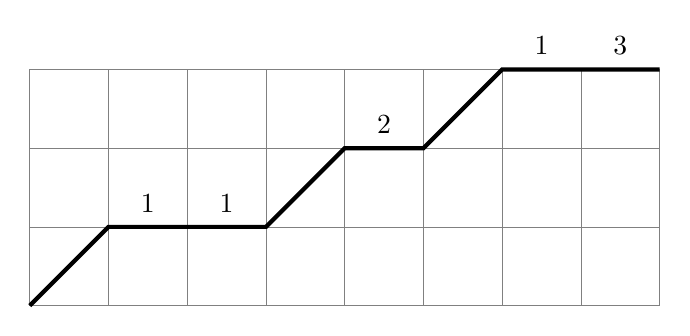
\begin{tikzpicture}
\draw[help lines] (0,0) grid (8,3);
\draw[line width = 1.5pt] (0,0) -- ++(1,1) -- ++(1,0) -- ++(1,0) -- ++(1,1) -- ++(1,0) -- ++(1,1) -- ++(1,0) -- ++(1,0);
\hlabel111 \hlabel211 \hlabel422 \hlabel631 \hlabel733 
\end{tikzpicture}
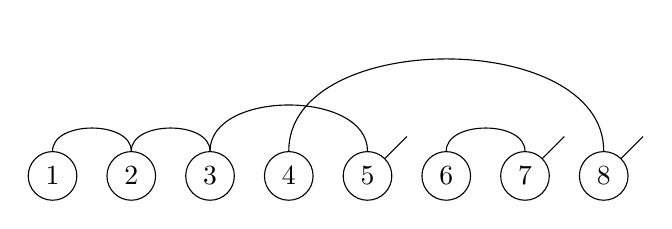
\begin{tikzpicture}
\begin{scope}[shift={(0,0)}]
\draw (5,0) -- (5.5,0.5);
\draw (7,0) -- (7.5,0.5);
\draw (8,0) -- (8.5,0.5);
\node[draw, circle,fill=white] (1) at (1,0) {\( 1 \)};
\node[draw, circle,fill=white] (2) at (2,0) {\( 2 \)};
\node[draw, circle,fill=white] (3) at (3,0) {\( 3 \)};
\node[draw, circle,fill=white] (5) at (5,0) {\( 5 \)};
\draw[out=90,in=90] (1) to (2);
\draw[out=90,in=90] (2) to (3);
\draw[out=90,in=90] (3) to (5);
\node[draw, circle,fill=white] (4) at (4,0) {\( 4 \)};
\node[draw, circle,fill=white] (8) at (8,0) {\( 8 \)};
\draw[out=90,in=90] (4) to (8);
\node[draw, circle,fill=white] (6) at (6,0) {\( 6 \)};
\node[draw, circle,fill=white] (7) at (7,0) {\( 7 \)};
\draw[out=90,in=90] (6) to (7);
\end{scope}

\end{tikzpicture}
\caption{A partial Charlier history (top) and the corresponding set
  partition, where every block has a half edge attached at the end
  (bottom).}
  \label{fig:Charlier-history-1}
\end{figure}

  Since \( b_k=k+1 \) and \( \lambda_k = k \), we have
  \[
    \sum_{k=0}^n \nu_{n,k}x^k = \sum_{T\in\FT_n} \wt(T)
    = x(x-1)(x-2) \cdots (x-n+1).
  \]
  On the other hand, by \eqref{eq:c(n,k)-gf}, we have
  \[
       \sum_{k=0}^n s(n,k)x^k = x(x-1)(x-2) \cdots (x-n+1).
  \]
  This proves the second identity also holds.
\end{proof}


\chapter{Determinants of moments}

We have learned that \( \mu_n \) can be written using \( b_n \) and
\( \lambda_n \). Since a monic OPS \( \{ P_n(x) \}_{n\ge 0} \) (and
hence the recurrence coefficients \( b_n \) and \( \lambda_n \) as
well) is uniquely determined by \( \mu_n \), there must be a way to
express \( b_n \) and \( \lambda_n \) using \( \mu_n \). In this
chapter we find such an expression using nonintersecting lattice paths
and the Lindstr\"om--Gessel--Viennot lemma.

\section{Computing the 3-term recurrence coefficients}

Let us first see how one can compute \( \mu_n \) using \( b_n \) and
\( \lambda_n \) for small \( n \). Recall
\[
  \mu_n = \sum_{\pi\in \Motz_n} \wt(\pi).
\]
Thus, the first few moments are
\begin{align*}
  \mu_1 &= b_0,\\
  \mu_2 &= b_0^2 + \lambda_1,\\
  \mu_3 &= b_0^3 + 2b_0\lambda_1 + b_1\lambda_1.
\end{align*}
Then we can solve for \( b_n \) and \( \lambda_n \):
\begin{align*}
  b_0  &= \mu_1, \\
  \lambda_1 &=  \mu_2 - b_0^2 = \mu_2 - \mu_1^2, \\
  b_1 &=  (\mu_3 -b_0^3 + 2b_0\lambda_1)/\lambda_1
        = (\mu_3 -\mu_1^3 + 2\mu_1(\mu_2-\mu_1^2))/(\mu_2 - \mu_1^2),
\end{align*}
and so on. Although, the formula gets very complicated, we can
convince ourselves that this always gives a formula for \( b_n \) and
\( \lambda_n \). We prove this rigorously as follows.

Suppose that we have computed \( b_0,\dots,b_{n-1} \) and
\( \lambda_1,\dots,\lambda_n \). Then in the sum
\[
  \mu_{2n+1} = \sum_{\pi\in \Motz_{2n+1}} \wt(\pi),
\]
\( b_n \) appears only once as \( b^n \lambda_n \lambda_{n-1} \cdots \lambda_1 \)
for the Motzkin path \( U^n H D_n \). Thus
\begin{equation}\label{eq:38}
  b^n \lambda_n \lambda_{n-1} \cdots \lambda_1
  = \mu_{2n+1} - \sum_{\pi\in \Motz_{2n+1}, \pi\ne U^n H D_n} \wt(\pi).
\end{equation}
Since the sum on the right-hand side of \eqref{eq:38} has only
\( b_0,\dots,b_{n-1} \) and \( \lambda_1,\dots,\lambda_n \), we can
express it using \( \mu_k \)'s. Then dividing both sides of
\eqref{eq:38} by \( \lambda_1 \cdots \lambda_n \), which can also be
written using \( \mu_k \)'s, we obtain a formula for \( b_n \) in
terms of \( \mu_k \)'s.

Similarly, if we have computed \( b_0,\dots,b_{n} \) and
\( \lambda_1,\dots,\lambda_n \), then we can find a formula for
\( \lambda_{n+1} \) in terms of \( \mu_k \)'s using
\[
  \mu_{2n+2} = \sum_{\pi\in \Motz_{2n+2}} \wt(\pi),
\]
because \( \lambda_{n+1} \) appears only once for the path
\( U^{n+1}D^{n+1} \).

The above algorithm shows that it is possible to express \( b_n \) and
\( \lambda_n \) using \( \mu_n \). To find an explicit formula, we
need to develop some interesting theory of lattice paths.


\section{The Lindstr\"om--Gessel--Viennot lemma}

The Lindstr\"om--Gessel--Viennot lemma \cite{Lindstrom,GesselViennot}
is a very useful tool in combinatorics. This lemma is listed in the
book called ``Proofs from The Book'' \cite[Chapter~32]{Aigner2018},
which tries to collect the most beautiful proofs in mathematics. We
start with basic definitions on paths in a directed graph.


\begin{defn}\label{def:5}
  A \emph{graph} is a pair \( G= (V,E) \) of two sets \( V \) and
  \( E \) such that \( E\subseteq V\times V \). Each element
  \( v\in V \) is called a \emph{vertex} and each element
  \( (u,v)\in E \) is called an \emph{edge}. We say that \( G \) is
  \emph{undirected} if \( (u,v) \) is identified with \( (v,u) \).
  Otherwise, \( G \) is said to be \emph{directed}.

  A \emph{path} from \( u \) to \( v \) is a sequence of vertices
  \( (v_0,v_1,\dots,v_n) \) such that \( v_0=u \), \( v_n=v \), and
  \( (v_i,v_{i+1})\in E \) for all \( 0\le i\le n-1 \). A \emph{cycle}
  is a path from a vertex to itself. For two vertices \( u \) and
  \( v \), we denote by \( P(u\to v) \) the set of paths from \( u \)
  to \( v \). If there is no cycle, \( G \) is said to be
  \emph{acyclic}. 

  An \emph{edge weight} of \( G \) is a function \( w:E \to K \), for
  some commutative ring \( K \). The \emph{weight} of a path \( p \)
  is defined to be the product of \( w(e) \) for every edge \( e \) in
  \( p \).
\end{defn}


We consider families of paths. For brevity, we define an
\emph{\( n \)-path} to be just an \( n \)-tuple
\( \vec p = (p_1,\dots,p_n) \) of paths. We say that two paths \( p \)
and \( p' \) are \emph{nonintersecting} if they do not have a common
vertex. We also say that an \( n \)-path
\( \vec p = (p_1,\dots,p_n) \) is \emph{nonintersecting} if \( p_i \)
and \( p_j \) are nonintersecting for all \( i\ne j \).

\begin{defn}\label{def:4}
  Let \( G \) be a directed graph with edge weight \( w \). Let
  \( \vec{A} = (A_1,\dots,A_n) \) and \( \vec B = (B_1,\dots,B_n) \)
  be sequences of vertices of \( G \). We denote by
  \( P(\vec A\to \vec B) \) the set of \( n \)-paths
  \( \vec p = (p_1,\dots,p_n) \) such that
  \( p_i\in P(A_i\to B_{\sigma(i)}) \), \( 1\le i\le n \), for some
  \( \sigma\in \sym_n \). We define
  \( w(\vec p) = w(p_1) \cdots w(p_n) \) and
  \( \sgn(\vec p)= \sgn(\sigma) \). Finally, we define
  \( \NI(\vec A\to \vec B) \) to be the set of all nonintersecting
  \( n \)-paths in \( P(\vec A\to \vec B) \).
\end{defn}

We are now ready to state the Lindstr\"om--Gessel--Viennot lemma.

\begin{thm}[The Lindstr\"om--Gessel--Viennot lemma]\label{thm:LGV}
  Let \( G \) be a directed graph with edge weight \( w \). Fix vertex
  sequences \( \vec A = (A_1,\dots,A_n) \) and
  \( \vec B = (B_1,\dots,B_n) \) and define the matrix
  \( M = (M_{i,j})_{i,j=1}^n \) by
\[
  M_{i,j} = \sum_{p\in P(A_i\to B_j)} w(p).
\]
Then we have
\[
  \det M = \sum_{\vec p \in \NI(\vec A \to \vec B)} \sgn(\vec p) w(\vec p).
\]
\end{thm}

Before proving this theorem let us consider an example.

\begin{exam}
  Let \( G \) be the directed graph whose vertex set \( V \)
  and (directed) edge set \( E \) are given by
  \begin{align*}
    V &= \{(i,j): 0\le i,j\le 2\},\\
    E &= \{(i,j)\to (i+1,j): 0\le i\le 1, 0\le j\le 2\}
        \cup \{(i,j)\to (i,j+1): 0\le i\le 2, 0\le j\le 1\}.
  \end{align*}
  Define the weight of every edge to be \( 1 \). Let
  \( \vec A = (A_1,A_2) \) and \( \vec B = (B_1,B_2) \), where
  \( A_1 = (0,0) \), \( A_2 = (1,0) \), \( B_1 = (1,2) \), and
  \( B_2 = (2,2) \). Then
  \[
  \det  M =
    \det \begin{pmatrix}
\binom{3}{1} & \binom{4}{2}\\[4pt]
\binom{2}{0} & \binom{3}{1}
\end{pmatrix}
= \det \begin{pmatrix}
3 & 6\\
1 & 3
\end{pmatrix} = 3.
  \]
  On the other hand, there are exactly \( 3 \) nonintersecting
  \( 2 \)-paths from \( \vec A \) to \( \vec B \) as shown in
  \Cref{fig:10}.
\end{exam}

\begin{figure}
  \centering
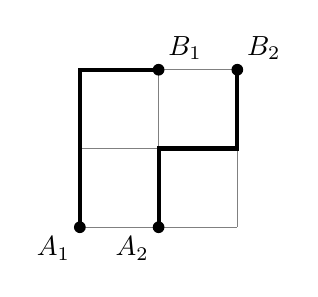
\begin{tikzpicture}
\draw[help lines] (0,0) grid (2,2);
\node at (0,0) [circle,fill,inner sep=1.5pt]{};
\node at (1,0) [circle,fill,inner sep=1.5pt]{};
\node at (1,2) [circle,fill,inner sep=1.5pt]{};
\node at (2,2) [circle,fill,inner sep=1.5pt]{};
\node [below left] at (0,0) {\( A_1 \)};
\node [below left] at (1,0) {\( A_2 \)};
\node [above right] at (1,2) {\( B_1 \)};
\node [above right] at (2,2) {\( B_2 \)};
\draw [line width=1.5pt] (0,0) -- (0,2) -- (1,2);
\draw [line width=1.5pt] (1,0) -- (1,1) -- (2,1) -- (2,2);
\end{tikzpicture} \qquad 
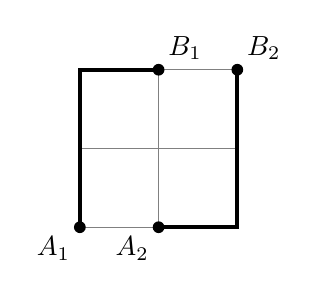
\begin{tikzpicture}
\draw[help lines] (0,0) grid (2,2);
\node at (0,0) [circle,fill,inner sep=1.5pt]{};
\node at (1,0) [circle,fill,inner sep=1.5pt]{};
\node at (1,2) [circle,fill,inner sep=1.5pt]{};
\node at (2,2) [circle,fill,inner sep=1.5pt]{};
\node [below left] at (0,0) {\( A_1 \)};
\node [below left] at (1,0) {\( A_2 \)};
\node [above right] at (1,2) {\( B_1 \)};
\node [above right] at (2,2) {\( B_2 \)};
\draw [line width=1.5pt] (0,0) -- (0,2) -- (1,2);
\draw [line width=1.5pt] (1,0) -- (2,0) -- (2,2);
\end{tikzpicture} \qquad 
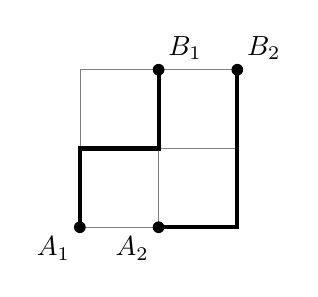
\begin{tikzpicture}
\draw[help lines] (0,0) grid (2,2);
\node at (0,0) [circle,fill,inner sep=1.5pt]{};
\node at (1,0) [circle,fill,inner sep=1.5pt]{};
\node at (1,2) [circle,fill,inner sep=1.5pt]{};
\node at (2,2) [circle,fill,inner sep=1.5pt]{};
\node [below left] at (0,0) {\( A_1 \)};
\node [below left] at (1,0) {\( A_2 \)};
\node [above right] at (1,2) {\( B_1 \)};
\node [above right] at (2,2) {\( B_2 \)};
\draw [line width=1.5pt] (0,0) -- (0,1) -- (1,1) -- (1,2);
\draw [line width=1.5pt] (1,0) -- (2,0) -- (2,2);
\end{tikzpicture}
\caption{All nonintersecting \( 3 \)-paths from \( A_1,A_2 \) to
  \( B_1,B_2 \).}
  \label{fig:10}
\end{figure}


Note that in the above example, we can compute the number of
nonintersecting \( 2 \)-paths \( \vec p\in \NI(\vec A\to \vec B) \) as
follows. First, observe that if
\( \vec p = (p_1,p_2)\in \NI(\vec A\to \vec B) \), then
\( p_1 \in P(A_1 \to B_1) \) and \( p_2 \in P(A_2 \to B_2) \). Thus
\( \NI(\vec A\to \vec B) \) is contained in the set
\( P(A_1 \to B_1) \times P(A_2 \to B_2) \) whose cardinality is
\( \binom{3}{1}\binom{3}{1} \). So, if we subtract the number of
intersecting \( 2 \)-paths
\( (p_1,p_2)\in P(A_1 \to B_1) \times P(A_2 \to B_2) \), we would get
the cardinality of \( \NI(\vec A\to \vec B) \).

Suppose that \( (p_1,p_2)\in P(A_1 \to B_1) \times P(A_2 \to B_2) \)
is intersecting. Then we can find the first intersection point \( u \)
of \( p_1 \) and \( p_2 \). Then we can write \( p_1 = p_1'p_1'' \)
and \( p_2 = p_2'p_2'' \), where \( p_i' \) (resp.~\( p_i'' \)) is the
part of \( p_i \) before \( u \) (resp.~after \( u \)). By exchanging
the tails \( p_1'' \) and \( p_2'' \) we can construct a new
\( 2 \)-path \( (q_1,q_2) \), that is, \( q_1 = p_1'p_2'' \) and
\( q_2 = p_2'p_1'' \), see \Cref{fig:11}.

\begin{figure}
  \centering
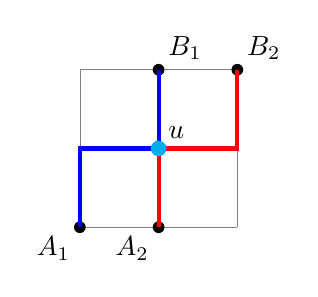
\begin{tikzpicture}
\draw[help lines] (0,0) grid (2,2);
\node at (0,0) [circle,fill,inner sep=1.5pt]{};
\node at (1,0) [circle,fill,inner sep=1.5pt]{};
\node at (1,2) [circle,fill,inner sep=1.5pt]{};
\node at (2,2) [circle,fill,inner sep=1.5pt]{};
\node [below left] at (0,0) {\( A_1 \)};
\node [below left] at (1,0) {\( A_2 \)};
\node [above right] at (1,2) {\( B_1 \)};
\node [above right] at (2,2) {\( B_2 \)};
\draw [line width=1.5pt,blue] (0,0) -- (0,1) -- (1,1) -- (1,2);
\draw [line width=1.5pt,red] (1,0) -- (1,1) -- (2,1) -- (2,2);
\node at (1,1) [cyan,circle,fill,inner sep=2pt]{};
\node [above right] at (1,1) {\( u \)};
\end{tikzpicture} \qquad 
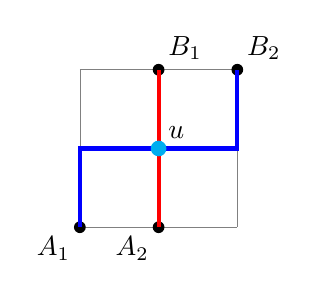
\begin{tikzpicture}
\draw[help lines] (0,0) grid (2,2);
\node at (0,0) [circle,fill,inner sep=1.5pt]{};
\node at (1,0) [circle,fill,inner sep=1.5pt]{};
\node at (1,2) [circle,fill,inner sep=1.5pt]{};
\node at (2,2) [circle,fill,inner sep=1.5pt]{};
\node [below left] at (0,0) {\( A_1 \)};
\node [below left] at (1,0) {\( A_2 \)};
\node [above right] at (1,2) {\( B_1 \)};
\node [above right] at (2,2) {\( B_2 \)};
\draw [line width=1.5pt,blue] (0,0) -- (0,1) -- (2,1) -- (2,2);
\draw [line width=1.5pt,red] (1,0) -- (1,2);
\node at (1,1) [cyan,circle,fill,inner sep=2pt]{};
\node [above right] at (1,1) {\( u \)};
\end{tikzpicture}
\caption{An intersecting \( 2 \)-path \( (p_1,p_2) \) and the
  corresponding \( 2 \)-path \( (q_1,q_2) \) obtained by exchanged the
  tails after the first intersection \( u \).}
\label{fig:11}
\end{figure}

Note that \( (q_1,q_2)\in P(A_1 \to B_2) \times P(A_2 \to B_1) \), and
any such \( 2 \)-path is always intersecting and thus gives rise to an
intersecting \( 2 \)-path
\( (p_1,p_2)\in P(A_1 \to B_1) \times P(A_2 \to B_2) \) by the same
process of exchanging the tails. Thus the number of intersecting
\( 2 \)-paths \( (p_1,p_2)\in P(A_1 \to B_1) \times P(A_2 \to B_2) \)
is equal to
\[
  |P(A_1 \to B_2) \times P(A_2 \to B_1)| = \binom{4}{2} \binom{2}{0}.
\]

We have just shown that
\[
  |\NI(\vec A\to \vec B)|  =
  \binom{3}{1}\binom{3}{1} - \binom{4}{2} \binom{2}{0}
=     \det \begin{pmatrix}
\binom{3}{1} & \binom{4}{2}\\[4pt]
\binom{2}{0} & \binom{3}{1}
           \end{pmatrix}.
\]
This idea of canceling intersecting \( 2 \)-paths can be extended to
prove \Cref{thm:LGV}.

\begin{proof}[Proof of \Cref{thm:LGV}]
  By definition,
\[
  \det M = \sum_{\sigma\in \sym_n} \sgn(\sigma) \prod_{i=1}^{n} M_{i,\sigma(i)}
  = \sum_{\sigma\in \sym_n} \sgn(\sigma) \sum_{p\in P(A_i\to B_{\sigma(i)})} w(p)
  = \sum_{\vec p \in P(\vec A\to \vec B)} \sgn(\vec p) w(\vec p).
\]
Thus it suffices to find a sign-reversing and weight-preserving
involution \( \phi \) on \( P(\vec A\to \vec B) \) with fixed point
set \( \NI(\vec A\to \vec B) \).

Consider an \( n \)-path
\( \vec p = (p_1,\dots,p_n)\in P(\vec A\to \vec B) \) with
\( p_i\in P(A_i\to B_{\sigma(i)}) \) for some \( \sigma\in \sym_n \).
If \( \vec p \) is nonintersecting, then define
\( \phi(\vec p) = \vec p \). Suppose now that \( \vec p \) is
intersecting. Then we can find the lexicographically smallest pair
\( (r,s) \) such that \( p_r \) and \( p_s \) are intersecting. We can
then find the first intersection point, say \( u \), of \( p_r \) and
\( p_s \). Let \( p'_r \) and \( p'_s \) to be the paths obtained from
\( p_r \) and \( p_s \) by exchanging their tails after \( u \).
We define \( \phi(\vec p) = \vec q \), where
\[
  \vec q = (q_1,\dots,q_n) = (p_1,\dots, p_{r-1}, p'_r, p_{r+1},\dots,p_{s-1}, p'_s,
  p_{s+1},\dots,p_n).
\]
See \Cref{fig:12}.
\begin{figure}
  \centering
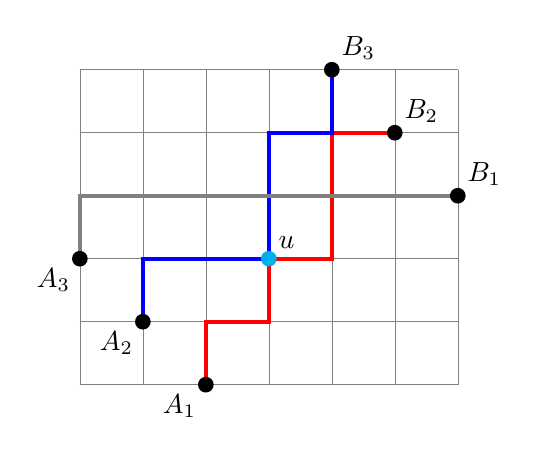
\begin{tikzpicture}[scale=0.8]
\draw[help lines] (0,0) grid (6,5);
\draw[red,line width = 1.5pt] (2,0) -- ++(0,1) -- ++ (1,0)-- ++ (0,1)-- ++ (1,0) -- ++ (0,2) -- ++ (1,0);
\draw[blue,line width = 1.5pt] (1,1) -- ++(0,1) -- ++ (2,0) -- ++ (0,2) -- ++ (1,0)-- ++ (0,1);
\draw[gray,line width = 1.5pt] (0,2) -- ++(0,1) -- ++ (6,0);
\node at (2,0) [circle,fill,inner sep=2pt]{};
\node at (1,1) [circle,fill,inner sep=2pt]{};
\node at (0,2) [circle,fill,inner sep=2pt]{};
\node at (6,3) [circle,fill,inner sep=2pt]{};
\node at (5,4) [circle,fill,inner sep=2pt]{};
\node at (4,5) [circle,fill,inner sep=2pt]{};
\node at (3,2) [cyan,circle,fill,inner sep=2pt]{};
\node [above right] at (3,2) {\( u \)};
\node [below left] at (2,0) {\( A_1 \)};
\node [below left] at (1,1) {\( A_2 \)};
\node [below left] at (0,2) {\( A_3 \)};
\node [above right] at (6,3) {\( B_1 \)};
\node [above right] at (5,4) {\( B_2 \)};
\node [above right] at (4,5) {\( B_3 \)};
\end{tikzpicture} \qquad 
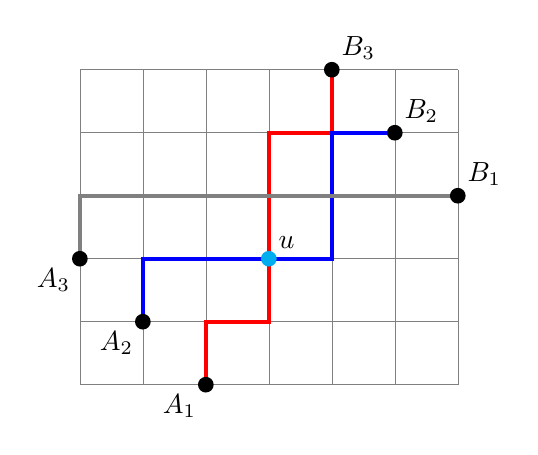
\begin{tikzpicture}[scale=0.8]
\draw[help lines] (0,0) grid (6,5);
\draw[red,line width = 1.5pt] (2,0) -- ++(0,1) -- ++ (1,0)-- ++ (0,1) -- ++ (0,2) -- ++ (1,0)-- ++ (0,1);
\draw[blue,line width = 1.5pt] (1,1) -- ++(0,1) -- ++ (2,0)-- ++ (1,0) -- ++ (0,2) -- ++ (1,0);
\draw[gray,line width = 1.5pt] (0,2) -- ++(0,1) -- ++ (6,0);
\node at (2,0) [circle,fill,inner sep=2pt]{};
\node at (1,1) [circle,fill,inner sep=2pt]{};
\node at (0,2) [circle,fill,inner sep=2pt]{};
\node at (6,3) [circle,fill,inner sep=2pt]{};
\node at (5,4) [circle,fill,inner sep=2pt]{};
\node at (4,5) [circle,fill,inner sep=2pt]{};
\node at (3,2) [cyan,circle,fill,inner sep=2pt]{};
\node [above right] at (3,2) {\( u \)};
\node [below left] at (2,0) {\( A_1 \)};
\node [below left] at (1,1) {\( A_2 \)};
\node [below left] at (0,2) {\( A_3 \)};
\node [above right] at (6,3) {\( B_1 \)};
\node [above right] at (5,4) {\( B_2 \)};
\node [above right] at (4,5) {\( B_3 \)};
\end{tikzpicture}
\caption{The involution \( \phi \) exchanges the tails of \( p_1 \)
  and \( p_2 \) after their first intersection point \( u \).}
  \label{fig:12}
\end{figure}

Since \( \vec p \) and \( \vec q \) have the same set of edges (with
the same multiplicities), we have \( w(\vec p) = w(\vec q) \). Since
\(p_i\in P(A_i\to B_{\sigma(i)}) \), we have
\(q_i\in P(A_i\to B_{\sigma'(i)}) \), where \( \sigma' \) is the
permutation obtained from \( \sigma = \sigma_1 \cdots \sigma_n \) by
exchanging \( \sigma_i \) and \( \sigma_j \). In other words,
\( \sigma'=\sigma (i,j) \), hence
\[
  \sgn(\vec p') = \sgn(\sigma') = \sgn(\sigma) = \sgn(\vec p).
\]
Moreover, by the construction of \( \phi \), it is clearly an
involution. Thus, \( \phi \) is a sign-reversing and weight-preserving
involution \( \phi \) on \( P(\vec A\to \vec B) \) with fixed point
set \( \NI(\vec A\to \vec B) \), which completes the proof.
\end{proof}

\begin{cor}\label{cor:LGV}
  Let \( G \) be a directed graph with edge weight \( w \). Fix vertex
  sequences \( \vec A = (A_1,\dots,A_n) \) and
  \( \vec B = (B_1,\dots,B_n) \) and define the matrix
  \( M = (M_{i,j})_{i,j=1}^n \) by
\[
  M_{i,j} = \sum_{p\in P(A_i\to B_j)} w(p).
\]
Suppose that  every nonintersecting \( n \)-path 
\( \vec p = (p_1,\dots,p_n)\in \NI(\vec A \to \vec B) \)
satisfies \( p_i \in P(A_i\to B_i) \) for all \( 1\le i\le n \).
Then 
\[
  \det M = \sum_{\vec p \in \NI(\vec A \to \vec B)} w(\vec p).
\]
In particular, if \( w(e) = 1 \) for all \( e\in E \), then the number
of nonintersecting \( n \)-paths is
\[
  |\NI(\vec A \to \vec B)| = \det M.
\]
\end{cor}

\begin{exam}
  The graph in \Cref{fig:12} and the vertices \( (A_1,A_2,A_3) \)
  and \( (B_1,B_2,B_3) \) satisfy the conditions in \Cref{cor:LGV}.
  Thus The number of nonintersecting \( 3 \)-paths from
  \( (A_1,A_2,A_3) \) and \( (B_1,B_2,B_3) \) is
  \[
    \det
    \begin{pmatrix}
\binom{7}{4} & \binom{7}{3} & \binom{7}{2}\\[4pt]
\binom{7}{5} & \binom{7}{4} & \binom{7}{3}\\[4pt]
\binom{7}{6} & \binom{7}{5} & \binom{7}{4}
\end{pmatrix} = 4116.
  \]
\end{exam}

\begin{exam}
  Not every directed graph and vertex sequences satisfy the conditions
  in \Cref{cor:LGV}. See~\Cref{fig:13}.
  In this case,
  \[
   \det M =  \det
    \begin{pmatrix}
\binom{4}{2} & \binom{6}{3}\\[4pt]
\binom{2}{1} & \binom{4}{2}
\end{pmatrix} = -4.
  \]
  Note that the number of nonintersecting \( 2 \)-paths
  \( (p_1,p_2) \) with \( p_i\in P(A_i\to B_{\sigma(i)}) \) is \( 2 \)
  if \( \sigma = 12 \) and \( 6 \) if \( \sigma = 21 \).
  This is in agreement of the Lindstr\"om--Gessel--Viennot lemma:
  \[
    \sgn(12) \cdot 2 + \sgn(21) \cdot 6 = 2-6 = -4.
  \]
\end{exam}

\begin{figure}
  \centering
\begin{tikzpicture}[scale=0.8]
\draw[help lines] (0,0) grid (3,3);
\draw[red,line width = 1.5pt] (1,1) -- ++(2,0) -- ++ (0,2);
\draw[blue,line width = 1.5pt] (0,0) -- ++(0,2) -- ++ (2,0);
\node at (0,0) [circle,fill,inner sep=2pt]{};
\node at (1,1) [circle,fill,inner sep=2pt]{};
\node at (2,2) [circle,fill,inner sep=2pt]{};
\node at (3,3) [circle,fill,inner sep=2pt]{};
\node [below left] at (0,0) {\( A_1 \)};
\node [below left] at (1,1) {\( A_2 \)};
\node [above right] at (2,2) {\( B_1 \)};
\node [above right] at (3,3) {\( B_2 \)};
\end{tikzpicture} \qquad 
\begin{tikzpicture}[scale=0.8]
\draw[help lines] (0,0) grid (3,3);
\draw[red,line width = 1.5pt] (1,1) -- ++(1,0) -- ++ (0,1);
\draw[blue,line width = 1.5pt] (0,0) -- ++(0,3) -- ++ (3,0);
\node at (0,0) [circle,fill,inner sep=2pt]{};
\node at (1,1) [circle,fill,inner sep=2pt]{};
\node at (2,2) [circle,fill,inner sep=2pt]{};
\node at (3,3) [circle,fill,inner sep=2pt]{};
\node [below left] at (0,0) {\( A_1 \)};
\node [below left] at (1,1) {\( A_2 \)};
\node [above right] at (2,2) {\( B_1 \)};
\node [above right] at (3,3) {\( B_2 \)};
\end{tikzpicture}
\caption{Two nonintersecting \( 2 \)-paths \( (p_1,p_2) \) and
  \( (q_1,q_2) \) with different connecting patterns.}
\label{fig:13}
\end{figure}

\begin{remark}
What if \( A_i=A_j \) or \( B_i=B_j \) for some \( i\ne j \)? Then
clearly there is no nonintersecting \( n \)-path from \( \vec A \)
to \( \vec B \). Thus, \( \det M = 0 \). This can also be seen
immediately from the definition of the matrix \( M \). For example,
if \( A_i=A_j \) then row \( i \) and row \( j \) of \( M \) are
identical so, \( \det M = 0 \).
\end{remark}

\begin{remark}
What if \( A_i=B_j \) for some \( i\ne j \)? Then every
nonintersecting \( n \)-path \( \vec p = (p_1,\dots,p_{n}) \) must
satisfy \( p_i \in P(A_i \to B_j) \). To see this suppose
\( p_i \in P(A_i \to B_k) \) for some \( k\ne j \). Then there is a
path \( p_r\in P(A_r\to B_j) \) for some \( r\ne i \). Then \( p_i \)
and \( p_r \) have a common vertex \( A_i = B_j \), a
contradiction.

Note also that if \( A_i=B_j \), then \( p_i \in P(A_i \to B_j) \)
means that \( p_i=(A_i) \) is a path of length \( 0 \), i.e., a path
with no edges. Hence, if \( \vec p = (p_1,\dots,p_{n}) \) is
nonintersecting, then every path other than \( p_i \) does not touch
the vertex \( A_i \). This can be used to find the number of paths
in \( G \) from \( u \) to \( v \) avoiding a given list of
vertices.
\end{remark}

\begin{exam}
  Let \( G \) be a directed graph with vertices
  \( A_1,\dots,A_n, B_1,\dots,B_n \) and edges \( (A_i,B_j) \) for
  \( 1\le i,j\le n \) with edge weight \( w \). Let
  \( \vec A = (A_1,\dots,A_n) \) and \( \vec B = (B_1,\dots,B_n) \).
  Then each \( P(A_i\to B_j) \) has only one path \( (A_i,B_j) \) with
  only one edge and every path \( \vec p \in P(\vec A \to \vec B) \)
  is nonintersecting. Thus the matrix \( M=(M_{i,j}) \) has entries
  \[
    M_{i,j} = \sum_{p\in P(A_i\to B_j)} w(p) = w(A_i,B_j).
  \]
  Then the Lindstr\"om--Gessel--Viennot lemma says
  \begin{align*}
    \det M
    &= \sum_{\vec p \in \NI(\vec A \to \vec B)} \sgn(\vec p) w(\vec p)
    = \sum_{\vec p \in P(\vec A \to \vec B)} \sgn(\vec p) w(\vec p)\\
    &= \sum_{\sigma\in\sym_n} \sgn(\sigma) \prod_{i=1}^{n} w(A_i,B_{\sigma(i)})
    = \sum_{\sigma\in\sym_n} \sgn(\sigma) \prod_{i=1}^{n} M_{i,j},
  \end{align*}
  which is nothing but the definition of the determinant of a matrix.
\end{exam}

There is an interesting application of the
Lindstr\"om--Gessel--Viennot lemma to a useful determinant identity
called the Cauchy--Binet formula.

\begin{defn}\label{def:6}
  Let \( M = (M_{i,j})_{i\in [m], j\in [n]} \) be an \( m\times n \)
  matrix. We denote by \( \binom{[m]}{k} \) the set of all subsets of
  \( [m] \) with cardinality \( k \). For
  \( I\subseteq \binom{[m]}{k} \) and \( J\subseteq \binom{[n]}{k} \),
  the \( (I,J) \)-minor \( [M]_{I,J} \) of \( M \) 
  is defined by
  \[
    [M]_{I,J} = \det (M_{i,j})_{i\in I,j\in J}.
  \]
\end{defn}

\begin{thm}[The Cauchy--Binet formula]\label{thm:7}
  Let \( M \) be an \( n\times \ell \) matrix let \( N \) be an
  \( \ell\times n \) matrix.
  Then
  \[
    \det (MN) = \sum_{I\in \binom{[\ell]}{n}} [M]_{[n],I} [N]_{I,[n]}.
  \]
\end{thm}

\begin{proof}
Let \( G \) be the directed graph with vertex set \( V \)
and edge set \( E \) given by
\begin{align*}
  V &= \{A_1,\dots,A_n, B_1,\dots,B_\ell, C_1,\dots,C_n\}, \\
  E &= \{(A_i,B_j): i\in [n], j\in [\ell]\} \cup
      \{(B_i,C_j): i\in [\ell], j\in [n]\}.
\end{align*}
Define an edge weight \( w \) of \( G \) by
\[
  w(A_i,B_j) = M_{i,j}, \qquad w(B_i,C_j) = N_{i,j}.
\]

Consider the \( n\times n \) matrix \( L=(L_{i,j})_{i,j\in[n]} \)
whose \( (i,j) \)-entry is
\[
  L_{i,j} = \sum_{p\in P(A_i\to C_j)} w(p).
\]
Since the above sum is equal to
\[
    \sum_{k=1}^{\ell} w(A_i,B_k) w(B_k,C_j)
  = \sum_{k=1}^{\ell} M_{i,k} N_{k,j} = (MN)_{i,j},
\]
we have \( L = MN \). Letting \( \vec A = (A_1,\dots,A_n) \) and
\( \vec C = (C_1,\dots,C_n) \), the Lindstr\"om--Gessel--Viennot lemma
implies
\[
  \det L = \sum_{\vec p\in \NI(\vec A \to \vec C)} 
  \sgn(\vec p) w(\vec p).
\]

Observe that every
\( \vec p = (p_1,\dots,p_{n})\in \NI(\vec A \to \vec C) \) is of the
form \( p_i = (A_i, B_{I_{\tau(i)}}, C_{\sigma(i)}) \) for some
\( I = \{I_1 < \cdots <I_n\}\in \binom{[\ell]}{n} \) and
\( \tau,\sigma\in \sym \). In this case
\( \sgn(\vec p) = \sgn(\sigma) \) and we can write
\( \sigma=\rho\tau \) for some \( \rho\in \sym_n \), in fact,
\( \rho = \sigma\tau^{-1} \).
Therefore
\begin{align*}
  \det L
  &= \sum_{I\in \binom{[\ell]}{n}} \sum_{\tau\in\sym_n} \sum_{\sigma\in\sym_n}  \sgn(\sigma) \prod_{i=1}^{n} w(A_i,B_{I_{\tau(i)}}, C_{\sigma(i)})\\
  &= \sum_{I\in \binom{[\ell]}{n}} \sum_{\tau\in\sym_n} \sum_{\rho\in\sym_n}  \sgn(\rho\tau) \prod_{i=1}^{n} w(A_i,B_{I_{\tau(i)}}, C_{\rho\tau(i)})\\
  &= \sum_{I\in \binom{[\ell]}{n}} \sum_{\tau\in\sym_n} \sgn(\tau) \left( \prod_{i=1}^{n} w(A_i,B_{I_{\tau(i)}}) \right)
    \sum_{\rho\in\sym_n}  \sgn(\rho) \left( \prod_{i=1}^{n} w(B_{I_{\tau(i)}}, C_{\rho\tau(i)}) \right)\\
  &= \sum_{I\in \binom{[\ell]}{n}} \sum_{\tau\in\sym_n} \sgn(\tau) \left( \prod_{i=1}^{n} w(A_i,B_{I_{\tau(i)}}) \right)
    \sum_{\rho\in\sym_n}  \sgn(\rho) \left( \prod_{i=1}^{n} w(B_{I_i}, C_{\rho(i)}) \right)\\
  &= \sum_{I\in \binom{[\ell]}{n}} \sum_{\tau\in\sym_n} \sgn(\tau) \left( \prod_{i=1}^{n} M_{i,I_{\tau(i)}} \right)
    \sum_{\rho\in\sym_n}  \sgn(\rho) \left( \prod_{i=1}^{n} N_{I_i,\rho(i)} \right)\\
  &= \sum_{I\in \binom{[\ell]}{n}} [M]_{[n],I} [N]_{I,[n]}.
\end{align*}
Since \( L=MN \), the proof is completed.
\end{proof}

\section{Hankel determinants of moments}

In this section we compute the Hankel determinants of moments using
the Lindstr\"om--Gessel--Viennot lemma.

As usual let \( \{ P_n(x) \}_{n\ge 0} \) be a monic OPS
satisfying
\[
  P_{n+1}(x) = (x-b_n) P_n(x) - \lambda_n P_{n-1}(x),
\]
and let \( \mu_n \) be the \( n \)th moment.


\begin{defn}\label{def:7}
  The (infinite) \emph{Hankel matrix} \( H \) of the sequence
  \( \{ \mu_n\}_{n\ge 0} \) is defined by
  \[
    H = \left( \mu_{i+j} \right)_{i,j=0}^\infty.
  \]
  The \emph{Hankel determinant} \( \Delta_n \) is defined by
\[
  \Delta_n = [H]_{\{0,1,\dots,n\},\{0,1,\dots,n\}} = \det \left(
    \mu_{i+j} \right)_{i,j=0}^n = \det
 \begin{pmatrix}
   \mu_0 & \mu_1 & \cdots & \mu_n\\
   \mu_1 & \mu_2 & \cdots & \mu_{n+1}\\
   \vdots & \vdots & \ddots & \vdots\\
   \mu_n & \mu_{n+1} & \cdots & \mu_{2n}
 \end{pmatrix}.
\]
\end{defn}

We will use the convention that the determinant of an empty matrix is
\( 1 \). For example, \( \Delta_{n} = 1 \) for \( n<0 \).

Note that \( \mu_{i+j} \) is the generating function for Motzkin paths
of length \( i+j \) with starting and ending heights \( 0 \). Let
\( \vec A = (A_0,\dots,A_n) \) and \( \vec B = (B_0,\dots,_n) \),
where \( A_i = (-i,0) \) and \( B_i = (i,0) \). Then
\[
  \mu_{i+j} = \sum_{p\in \Motz(A_i\to B_j)} \wt(p).
\]
Therefore, by \Cref{thm:LGV},
\[
  \Delta_n = \det \left( \mu_{i+j} \right)_{i,j=0}^n = \sum_{\vec p
    \in \NI(\vec A \to \vec B)} \sgn(\vec p) \wt(\vec p).
\]
But, \( \NI(\vec A \to \vec B) \) has a unique \( (n+1) \)-path
\( \vec p = (p_0,\dots,p_n) \) as shown in \Cref{fig:14}.
Observe that \( \wt(\vec p) = \lambda_1^n \lambda_2^{n-1} \cdots \lambda_n^1 \).
This shows the following theorem.

\begin{figure}
  \centering
\begin{tikzpicture}
\draw[help lines] (0,0) grid (6,3);
\draw node at (3,-.5) {\( A_0=B_0 \)};
\draw node at (2,-.5) {\( A_1 \)};
\draw node at (1,-.5) {\( A_2 \)};
\draw node at (0,-.5) {\( A_3 \)};
\draw node at (4,-.5) {\( B_1 \)};
\draw node at (5,-.5) {\( B_2 \)};
\draw node at (6,-.5) {\( B_3 \)};
\draw[line width = 1.5pt] (0,0) -- ++(1,1) -- ++(1,1) -- ++(1,1) -- ++(1,-1) -- ++(1,-1) -- ++(1,-1);
\draw[line width = 1.5pt] (1,0) -- ++(1,1) -- ++(1,1) -- ++(1,-1) -- ++(1,-1);
\draw[line width = 1.5pt] (2,0) -- ++(1,1) -- ++(1,-1);
\dlabel31{\lambda_1}
\dlabel32{\lambda_2}
\dlabel33{\lambda_3}
\dlabel41{\lambda_1}
\dlabel42{\lambda_2}
\dlabel51{\lambda_1}
\node at (0,0) [circle,fill,inner sep=2pt]{};
\node at (1,0) [circle,fill,inner sep=2pt]{};
\node at (2,0) [circle,fill,inner sep=2pt]{};
\node at (3,0) [circle,fill,inner sep=2pt]{};
\node at (4,0) [circle,fill,inner sep=2pt]{};
\node at (5,0) [circle,fill,inner sep=2pt]{};
\node at (6,0) [circle,fill,inner sep=2pt]{};
\end{tikzpicture}
\caption{The unique nonintersecting \( (n+1) \)-path in
  \( \NI(\vec A \to \vec B) \) for the case \( n=3 \).}
  \label{fig:14}
\end{figure}

\begin{thm}\label{thm:8}
  We have
  \[
    \Delta_n = \lambda_1^n \lambda_2^{n-1} \cdots \lambda_n^1.
  \]
\end{thm}


Now let's consider the following minor of the Hankel matrix:
\[
 \Delta'_n := [H]_{\{0,1,\dots,n\},\{0,1,\dots,n-1,n+1\}} = \det(M_{i,j})_{i,j=0}^n,
\]
where \( M_{i,j} = \mu_{i+j} \) if \( j<n \) and
\( M_{i,n} = \mu_{i+n+1} \). Let \( \vec A = (A_0,\dots,A_n) \) and
\( \vec B' = (B_0,\dots,B_n) \), where \( A_i = (-i,0) \) and
\( B_i = (i + \delta_{i,n},0) \). Then by the
Lindstr\"om--Gessel--Viennot lemma,
\[
  \Delta'_n = \sum_{\vec p \in \NI(\vec A \to \vec B')} \sgn(\vec p)
  \wt(\vec p).
\]
Suppose \( \vec p = (p_0,\dots,p_n)\in \NI(\vec A \to \vec B') \).
Then \( p_0,\dots,p_{n-1} \) are fixed as in the previous case.
Moreover, the first \( n \) steps of \( p_n \) must be all up steps.
Since \( p_n \) is a Motzkin path of length \( 2n+1 \), the remaining
steps are \( n \) down steps and one horizontal step. Thus
\( \wt(p_n) = \lambda_1 \cdots \lambda_n b_k \) for some
\( 0\le k\le n \) and \( p_n \) is determined by the number \( k \).
See \Cref{fig:15}. This shows the following theorem.

\begin{figure}
  \centering
\begin{tikzpicture}
\draw[help lines] (-1,0) grid (8,4);
\draw node at (3,-.5) {\( A_0=B_0 \)};
\draw node at (2,-.5) {\( A_1 \)};
\draw node at (1,-.5) {\( A_2 \)};
\draw node at (0,-.5) {\( A_3 \)};
\draw node at (-1,-.5) {\( A_4 \)};
\draw node at (4,-.5) {\( B_1 \)};
\draw node at (5,-.5) {\( B_2 \)};
\draw node at (6,-.5) {\( B_3 \)};
\draw node at (8,-.5) {\( B_4 \)};
\draw[line width = 1.5pt] (-1,0) -- ++(1,1) -- ++(1,1) -- ++(1,1) -- ++(1,1) -- ++(1,-1) -- ++(1,-1) -- ++(1,-1) --++(1,0) --++(1,-1);
\draw[line width = 1.5pt] (0,0) -- ++(1,1) -- ++(1,1) -- ++(1,1) -- ++(1,-1) -- ++(1,-1) -- ++(1,-1);
\draw[line width = 1.5pt] (1,0) -- ++(1,1) -- ++(1,1) -- ++(1,-1) -- ++(1,-1);
\draw[line width = 1.5pt] (2,0) -- ++(1,1) -- ++(1,-1);
\dlabel31{\lambda_1}
\dlabel32{\lambda_2}
\dlabel33{\lambda_3}
\dlabel34{\lambda_4}
\dlabel41{\lambda_1}
\dlabel42{\lambda_2}
\dlabel43{\lambda_3}
\dlabel52{\lambda_2}
\dlabel51{\lambda_1}
\dlabel71{\lambda_1}
\hlabel61{b_1}
\node at (-1,0) [circle,fill,inner sep=2pt]{};
\node at (0,0) [circle,fill,inner sep=2pt]{};
\node at (1,0) [circle,fill,inner sep=2pt]{};
\node at (2,0) [circle,fill,inner sep=2pt]{};
\node at (3,0) [circle,fill,inner sep=2pt]{};
\node at (4,0) [circle,fill,inner sep=2pt]{};
\node at (5,0) [circle,fill,inner sep=2pt]{};
\node at (6,0) [circle,fill,inner sep=2pt]{};
\node at (8,0) [circle,fill,inner sep=2pt]{};
\end{tikzpicture}
\caption{A nonintersecting \( (n+1) \)-path in
  \( \NI(\vec A \to \vec B') \) for the case \( n=4 \).}
\label{fig:15}
\end{figure}

\begin{thm}\label{thm:9}
  We have
  \[
    \Delta'_n = \lambda_1^n \lambda_2^{n-1} \cdots \lambda_n^1 (b_0 + \cdots + b_n)
    = \Delta_n (b_0 + \cdots + b_n).
  \]
\end{thm}

Using \Cref{thm:8} and \Cref{thm:9} we can express \( \lambda_n \) and
\( b_n \) using \( \mu_n \)'s as follows.

\begin{cor}\label{cor:3}
For \( n\ge1 \), we have
  \begin{align*}
    \lambda_n &= \frac{\Delta_n\Delta_{n-2}}{\Delta_{n-1}^2},\\
    b_n &= \frac{\Delta'_n}{\Delta_{n}} - \frac{\Delta'_{n-1}}{\Delta_{n-1}},
  \end{align*}
  and \( b_0 = \Delta'_0/\Delta_{0} \).
\end{cor}

\begin{proof}
By \Cref{thm:8}, \( \lambda_1 \cdots \lambda_n = \Delta_n/\Delta_{n-1} \).
Thus
\[
  \lambda_n = \frac{\Delta_n}{\Delta_{n-1}} \cdot \left(
    \frac{\Delta_{n-1}}{\Delta_{n-2}} \right)^{-1} =
  \frac{\Delta_n\Delta_{n-2}}{\Delta_{n-1}^2}.
\]
Similarly, by \Cref{thm:9},
\( b_0 + \cdots + b_n = \Delta'_n/\Delta_n \).
Thus
\[
  b_n = \frac{\Delta'_n}{\Delta_{n}} - \frac{\Delta'_{n-1}}{\Delta_{n-1}}.
  \qedhere
\]
\end{proof}

\begin{cor}\label{cor:4}
  Let \( \{ \mu_n\}_{n\ge 0} \) be a sequence of numbers. There is an
  OPS with moments \( \mu_n \) if and only if \( \Delta_n \ne 0 \) for
  all \( n \ge 0 \).
\end{cor}

\begin{proof}
  We know that \( \{ P_n(x) \}_{n\ge 0} \) is an OPS
  if and only if it satisfies a 3-term recurrence relation
  \begin{equation}\label{eq:39}
    P_{n+1}(x) = (x-b_n) P_n(x) - \lambda_n P_{n-1}(x)
  \end{equation}
  with \( \lambda_n\ne 0 \). Thus, if \( \{ P_n(x) \}_{n\ge 0} \) is
  an OPS, then by \Cref{thm:8}, \( \Delta_n\ne 0 \).

  Conversely, if \( \Delta_n\ne 0 \), then we can construct
  \( \lambda_n \) and \( b_n \) using \Cref{cor:3}. By the
  construction, \( \lambda_n \) and \( b_n \) are the sequences which
  give \( \mu_n = \sum_{p\in \Motz_n} \wt(p) \). Hence, if we define
  \( \{ P_n(x) \}_{n\ge 0} \) by \eqref{eq:39}, then it is an OPS with
  moments \( \mu_n \).
\end{proof}

For the rest of this section, we consider the case \( b_n=0 \). Recall
that \( \mu_{2n+1} = 0 \) for all \( n\ge0 \) if and only if
\( b_n=0 \) for all \( n\ge0 \). In this case there is a
correspondence between \( \{ \mu_{2n}\}_{n\ge 0} \) and
\( \{ \lambda_n\}_{n\ge 0} \). For example,
\begin{align*}
  \Delta_3
  & = \det 
  \begin{pmatrix}
\mu_0 & \mu_1 & \mu_2 & \mu_3 \\
\mu_1 & \mu_2 & \mu_3 & \mu_4 \\
\mu_2 & \mu_3 & \mu_4 & \mu_5 \\
\mu_3 & \mu_4 & \mu_5 & \mu_6 \\
\end{pmatrix} =\det 
  \begin{pmatrix}
\mu_0 & 0 & \mu_2 & 0 \\
0 & \mu_2 & 0 & \mu_4 \\
\mu_2 & 0 & \mu_4 & 0 \\
0 & \mu_4 & 0 & \mu_6 \\
\end{pmatrix}
= \det
\begin{pmatrix}
\mu_0 & \mu_2 \\
\mu_2 & \mu_4 \\
\end{pmatrix}
\det
\begin{pmatrix}
\mu_2 & \mu_4 \\
\mu_4 & \mu_6 \\
\end{pmatrix},\\
  \Delta_4
  &= \det 
  \begin{pmatrix}
\mu_0 & \mu_1 & \mu_2 & \mu_3 & \mu_4 \\
\mu_1 & \mu_2 & \mu_3 & \mu_4 & \mu_5 \\
\mu_2 & \mu_3 & \mu_4 & \mu_5 & \mu_6 \\
\mu_3 & \mu_4 & \mu_5 & \mu_6 & \mu_7 \\
\mu_4 & \mu_5 & \mu_6 & \mu_7 & \mu_8 \\
\end{pmatrix} =\det 
  \begin{pmatrix}
\mu_0 & 0 & \mu_2 & 0 & \mu_4 \\
0 & \mu_2 & 0 & \mu_4 & 0\\
\mu_2 & 0 & \mu_4 & 0 & \mu_6 \\
0 & \mu_4 & 0 & \mu_6 & 0 \\
\mu_4 & 0 & \mu_6 & 0 & \mu_8 \\
\end{pmatrix}\\
&= \det
\begin{pmatrix}
\mu_0 & \mu_2 & \mu_4 \\
\mu_2 & \mu_4 & \mu_6 \\
\mu_4 & \mu_6 & \mu_8 \\
\end{pmatrix}
\det
\begin{pmatrix}
\mu_2 & \mu_4 \\
\mu_4 & \mu_6 \\
\end{pmatrix}.
\end{align*}
In general, we have
\begin{align}
\label{eq:40}  \Delta_{2n} &= \Delta_n(2) \Delta^+_{n-1}(2),\\
  \Delta_{2n+1} &= \Delta_n(2) \Delta^+_{n}(2),
\end{align}
where
\begin{align*}
  \Delta_n(2) &= \det \left( \mu_{2i+2j} \right)_{i,j=0}^n,\\
  \Delta^+_n(2) &= \det \left( \mu_{2i+2j+2} \right)_{i,j=0}^n,\\
\end{align*}

Since \( b_n=0 \), we have
\[
  \mu_{2n} = \sum_{p\in \Dyck_{2n}} \wt(p).
\]
Let \( \vec A = (A_0,\dots,A_n) \) and \( \vec B = (B_0,\dots,B_n) \),
where \( A_i = (-2i,0) \) and \( B_i = (2i,0) \). Then
\[
  \mu_{2i+2j} = \sum_{p\in \Dyck(A_i\to B_j)} \wt(p). 
\]
Thus, by the Lindstr\"om--Gessel--Viennot lemma,
\[
  \Delta_n(2) = \sum_{\vec p \in \NI(\vec A \to \vec B)} \sgn(\vec p) \wt(\vec p).
\]
There is only one element in \( \NI(\vec A \to \vec B) \) as shown in
\Cref{fig:16}.
This gives the following theorem.

\begin{thm}\label{thm:11}
  If \( b_n=0 \) for all \( n\ge0 \), we have
\[
  \Delta_n(2) = (\lambda_1\lambda_2)^n (\lambda_3\lambda_4)^{n-1}
  \cdots  (\lambda_{2n-1}\lambda_{2n})^1.
\]
\end{thm}


\begin{figure}
  \centering
\begin{tikzpicture}
\draw[help lines] (0,0) grid (12,6);
\draw node at (6,-.5) {\( A_0=B_0 \)};
\draw node at (4,-.5) {\( A_1 \)};
\draw node at (2,-.5) {\( A_2 \)};
\draw node at (0,-.5) {\( A_3 \)};
\draw node at (8,-.5) {\( B_1 \)};
\draw node at (10,-.5) {\( B_2 \)};
\draw node at (12,-.5) {\( B_3 \)};
\draw[line width = 1.5pt] (0,0) -- ++(2,2) -- ++(2,2) -- ++(2,2) -- ++(2,-2) -- ++(2,-2) -- ++(2,-2);
\draw[line width = 1.5pt] (2,0) -- ++(2,2) -- ++(2,2) -- ++(2,-2) -- ++(2,-2);
\draw[line width = 1.5pt] (4,0) -- ++(2,2) -- ++(2,-2);
\node at (0,0) [circle,fill,inner sep=2pt]{};
\node at (2,0) [circle,fill,inner sep=2pt]{};
\node at (4,0) [circle,fill,inner sep=2pt]{};
\node at (6,0) [circle,fill,inner sep=2pt]{};
\node at (8,0) [circle,fill,inner sep=2pt]{};
\node at (10,0) [circle,fill,inner sep=2pt]{};
\node at (12,0) [circle,fill,inner sep=2pt]{};
\dlabel71{\lambda_1}
\dlabel{8}2{\lambda_2}
\dlabel73{\lambda_3}
\dlabel93{\lambda_3}
\dlabel{11}1{\lambda_1}
\dlabel{10}2{\lambda_2}
\dlabel{6}2{\lambda_2}
\dlabel91{\lambda_1}
\dlabel64{\lambda_4}
\dlabel84{\lambda_4}
\dlabel75{\lambda_5}
\dlabel{6}6{\lambda_6}
\end{tikzpicture}
\caption{The unique nonintersecting \( (n+1) \)-path in
  \( \NI(\vec A \to \vec B) \) for the case \( n=3 \).}
\label{fig:16}
\end{figure}


Now let \( \vec A = (A_0,\dots,A_n) \) and \( \vec B^+ = (B^+_0,\dots,B^+_n) \),
where \( A_i = (-2i,0) \) and \( B^+_i = (2i+2,0) \). Then
\[
  \mu_{2i+2j} = \sum_{p\in \Dyck(A_i\to B_j)} \wt(p). 
\]
Thus, by the Lindstr\"om--Gessel--Viennot lemma,
\[
  \Delta_n(2) = \sum_{\vec p \in \NI(\vec A \to \vec B)} \sgn(\vec p) \wt(\vec p).
\]
There is only one element in \( \NI(\vec A \to \vec B) \) as shown in
\Cref{fig:16}.
This gives the following theorem.
\begin{thm}\label{thm:12}
  If \( b_n=0 \) for all \( n\ge0 \), we have
\[
  \Delta^+_n(2) = \lambda_1^{n+1} (\lambda_2\lambda_3)^{n} (\lambda_4\lambda_5)^{n-1}
  \cdots  (\lambda_{2n}\lambda_{2n+1})^1.
\]
\end{thm}




\begin{figure}
  \centering
\begin{tikzpicture}
\draw[help lines] (0,0) grid (10,5);
\draw node at (4,-.5) {\( A_0 \)};
\draw node at (2,-.5) {\( A_1 \)};
\draw node at (0,-.5) {\( A_2 \)};
\draw node at (6,-.5) {\( B_0 \)};
\draw node at (8,-.5) {\( B_1 \)};
\draw node at (10,-.5) {\( B_2 \)};
\draw[line width = 1.5pt] (0,0) -- ++(5,5) -- ++(5,-5);
\draw[line width = 1.5pt] (2,0) -- ++(3,3) --++(3,-3);
\draw[line width = 1.5pt] (4,0) -- ++(1,1) -- ++(1,-1);
\node at (0,0) [circle,fill,inner sep=2pt]{};
\node at (2,0) [circle,fill,inner sep=2pt]{};
\node at (4,0) [circle,fill,inner sep=2pt]{};
\node at (6,0) [circle,fill,inner sep=2pt]{};
\node at (8,0) [circle,fill,inner sep=2pt]{};
\node at (10,0) [circle,fill,inner sep=2pt]{};
\dlabel51{\lambda_1}
\dlabel71{\lambda_1}
\dlabel{8}2{\lambda_2}
\dlabel73{\lambda_3}
\dlabel53{\lambda_3}
\dlabel{6}2{\lambda_2}
\dlabel91{\lambda_1}
\dlabel64{\lambda_4}
\dlabel55{\lambda_5}
\end{tikzpicture}
\caption{The unique nonintersecting \( (n+1) \)-path in
  \( \NI(\vec A \to \vec B^+) \) for the case \( n=2 \).}
\label{fig:17}
\end{figure}


\begin{cor}\label{cor:5}
  If \( b_n=0 \) for all \( n\ge0 \), we have
  \begin{align*}
  \lambda_{2n} &= \frac{\Delta_n(2)\Delta^+_{n-2}(2)}{\Delta_{n-1}(2)\Delta^+_{n-1}(2)}, \\
  \lambda_{2n+1} &= \frac{\Delta^+_n(2)\Delta_{n-1}(2)}{\Delta_{n}(2)\Delta^+_{n-1}(2)}.
  \end{align*}
\end{cor}

\begin{proof}
By \Cref{thm:11} and \ref{thm:12},
\[
\frac{\Delta^+_n(2)}{\Delta_{n}(2)}  = \lambda_1 \lambda_3 \cdots \lambda_{2n+1}, \qquad  
\frac{\Delta_n(2)}{\Delta^+_{n-1}(2)}  = \lambda_2 \lambda_4 \cdots \lambda_{2n}.
\]
Thus
\begin{align*}
  \lambda_{2n+1}
  &= \frac{\Delta^+_n(2)}{\Delta_{n}(2)} \left( \frac{\Delta^+_{n-1}(2)}{\Delta_{n-1}(2)} \right)^{-1}
    = \frac{\Delta^+_n(2)\Delta_{n-1}(2)}{\Delta_{n}(2)\Delta^+_{n-1}(2)},\\
  \lambda_{2n}
  &= \frac{\Delta_n(2)}{\Delta^+_{n-1}(2)} \left( \frac{\Delta_{n-1}(2)}{\Delta^+_{n-2}(2)} \right)^{-1}
    = \frac{\Delta_n(2)\Delta^+_{n-2}(2)}{\Delta_{n-1}(2)\Delta^+_{n-1}(2)}.
    \qedhere
\end{align*}

\end{proof}



\section{Another duality between moments and coefficients}

Recall that we proved a duality between mixed moments \( \mu_{n,k} \)
and coefficients \( \nu_{n,k} \). In this section we will prove the
following theorem, which gives another type of duality between moments
and coefficients.


\begin{thm}\label{thm:10}
  Let \( \LL \) be a linear functional with moment sequence
  \( \{\mu_n\} \) with \( \Delta_n\ne 0 \) for all \( n\ge0 \).
  Then the monic OPS for \( \LL \) is given by
  \[
    P_n(x) = \frac{1}{\Delta_{n-1}}
    \begin{vmatrix}
      \mu_0 & \mu_1 & \cdots & \mu_n\\
      \mu_1 & \mu_2 & \cdots & \mu_{n+1}\\
      \vdots & \vdots & \ddots & \vdots\\
      \mu_{n-1} & \mu_{n} & \cdots & \mu_{2n-1}\\
      1 & x & \cdots & x^n
    \end{vmatrix}.
  \]
\end{thm}

Let us write
\[
  P_n(x) = \sum_{k=0}^{n} \nu_{n,k} x^k.
\]
Then the theorem above is equivalent to
\begin{equation}\label{eq:41}
  \nu_{n,k} = \frac{(-1)^{n-k}}{\Delta_{n-1}}
  [H]_{\{0,\dots,n-1\}, \{0,\dots,k-1,k+1,\dots,n\}}.
 \end{equation}
Thus we need to compute
\[
   [H]_{\{0,\dots,n-1\}, \{0,\dots,k-1,k+1,\dots,n\}}
   = \det (\mu_{i+j+\chi(j\ge k)})_{i,j=0}^{n-1},
\]
where, for a statement \( P \), \( \chi(P)=1 \) if \( P \) is true and
\( \chi(P)=0 \) otherwise. Let \( \vec A = (A_0,\dots,A_{n-1}) \) and
\( \vec B^{(k)} = (B_0,\dots,B_{n-1}) \), where
\[
  A_i = (-i,0), \qquad B_i = (i + \chi(i\ge k),0).
\]
Then by the Lindstr\"om--Gessel--Viennot lemma,
\begin{equation}\label{eq:42}
  [H]_{\{0,\dots,n-1\}, \{0,\dots,k-1,k+1,\dots,n\}} = \sum_{\vec p
    \in \NI(\vec A \to \vec B^{(k)})} \sgn(\vec p) \wt(\vec p).
\end{equation}


\begin{figure}
  \centering
\begin{tikzpicture}[scale=1.2]
\draw[help lines] (-5,0) grid (6,5);
\draw node at (-5,-.5) {\( A_5 \)};
\draw node at (-4,-.5) {\( A_4 \)};
\draw node at (-3,-.5) {\( A_3 \)};
\draw node at (-2,-.5) {\( A_2 \)};
\draw node at (-1,-.5) {\( A_1 \)};
\draw node at (0,-.5) {\( A_0=B_0 \)};
\draw node at (1,-.5) {\( B_1 \)};
\draw node at (3,-.5) {\( B_2 \)};
\draw node at (4,-.5) {\( B_3 \)};
\draw node at (5,-.5) {\( B_4 \)};
\draw node at (6,-.5) {\( B_5 \)};
\draw[line width = 1.5pt] (-1,0) --++ (1,1) --++ (1,-1);
\draw[line width = 1.5pt] (-2,0) --++ (2,2) -- ++(1,-1) -- ++(1,1) -- ++(2,-2);
\draw[line width = 1.5pt] (-3,0) --++ (3,3) -- ++(3,-3);
\draw[line width = 1.5pt] (-4,0) --++ (4,4)  -- ++(1,0)-- ++(4,-4);
\draw[line width = 1.5pt] (-5,0) --++ (5,5)  -- ++(1,0)-- ++(5,-5);
\node at (0,0) [circle,fill,inner sep=2pt]{};
\node at (1,0) [circle,fill,inner sep=2pt]{};
\node at (3,0) [circle,fill,inner sep=2pt]{};
\node at (4,0) [circle,fill,inner sep=2pt]{};
\node at (5,0) [circle,fill,inner sep=2pt]{};
\node at (6,0) [circle,fill,inner sep=2pt]{};
\node at (-1,0) [circle,fill,inner sep=2pt]{};
\node at (-2,0) [circle,fill,inner sep=2pt]{};
\node at (-3,0) [circle,fill,inner sep=2pt]{};
\node at (-4,0) [circle,fill,inner sep=2pt]{};
\node at (-5,0) [circle,fill,inner sep=2pt]{};
\end{tikzpicture}
\caption{A nonintersecting \( (n+1) \)-path in
  \( \NI(\vec A \to \vec B^{(k)}) \) for the case \( n=6 \) and \( k=2 \).}
\label{fig:18}
\end{figure}

Now we investigate a nonintersecting \( (n+1) \)-path
\( \vec p = (p_0,\dots,p_{n-1}) \in \NI(\vec A \to \vec B^{(k)}) \),
see \Cref{fig:18} for an example. For \( 1\le i\le n-1 \), let
\( R_i \) be the region defined by
\[
  R_i = \{(x,y)\in\RR^2: x>0, i-1<y<i  \}.
\]
Then we have the following observations. See \Cref{fig:19}.

\begin{figure}
  \centering
\begin{tikzpicture}[scale=1.2]
\draw[help lines] (-5,0) grid (6,5);
\draw node at (-5,-.5) {\( A_5 \)};
\draw node at (-4,-.5) {\( A_4 \)};
\draw node at (-3,-.5) {\( A_3 \)};
\draw node at (-2,-.5) {\( A_2 \)};
\draw node at (-1,-.5) {\( A_1 \)};
\draw node at (0,-.5) {\( A_0=B_0 \)};
\draw node at (1,-.5) {\( B_1 \)};
\draw node at (3,-.5) {\( B_2 \)};
\draw node at (4,-.5) {\( B_3 \)};
\draw node at (5,-.5) {\( B_4 \)};
\draw node at (6,-.5) {\( B_5 \)};
\draw[line width = 1.5pt] (-1,0) --++ (1,1) --++ (1,-1);
\draw[line width = 1.5pt] (-2,0) --++ (2,2) -- ++(1,-1) -- ++(1,1) -- ++(2,-2);
\draw[line width = 1.5pt] (-3,0) --++ (3,3) -- ++(3,-3);
\draw[line width = 1.5pt] (-4,0) --++ (4,4)  -- ++(1,0)-- ++(4,-4);
\draw[line width = 1.5pt] (-5,0) --++ (5,5)  -- ++(1,0)-- ++(5,-5);
\node at (0,0) [circle,fill,inner sep=1pt]{};
\draw[dotted, red,line width = 2pt] (0,5) --++ (1,-1);
\draw[dotted, red,line width = 2pt] (0,4) --++ (1,-1);
\draw[dotted, red,line width = 2pt] (1,3) --++ (1,-1);
\draw[dotted, red,line width = 2pt] (1,2) --++ (1,-1);
\draw[dotted, red,line width = 2pt] (1,1) --++ (1,-1);
\draw[dotted, red,line width = 2pt] (1,1) --++ (1,1);
\node at (0,0) [circle,fill,inner sep=2pt]{};
\node at (1,0) [circle,fill,inner sep=2pt]{};
\node at (3,0) [circle,fill,inner sep=2pt]{};
\node at (4,0) [circle,fill,inner sep=2pt]{};
\node at (5,0) [circle,fill,inner sep=2pt]{};
\node at (6,0) [circle,fill,inner sep=2pt]{};
\node at (-1,0) [circle,fill,inner sep=2pt]{};
\node at (-2,0) [circle,fill,inner sep=2pt]{};
\node at (-3,0) [circle,fill,inner sep=2pt]{};
\node at (-4,0) [circle,fill,inner sep=2pt]{};
\node at (-5,0) [circle,fill,inner sep=2pt]{};
\end{tikzpicture}
\caption{The missing down steps and the figure ``X'' in \Cref{fig:18}
  are drawn with red dotted lined.}
\label{fig:19}
\end{figure}

\begin{enumerate}
\item The first \( i \) steps of \( p_i \) are up steps. Hence
  \( p_i \) visits \( (0,i) \).
\item There are \( n-i \) paths having at
  least one step in \( R_i \), namely,
  \( p_{i},p_{i+1},\dots,p_{n-1} \).
\item If \( d \) and \( u \) are the number of down steps and up steps
  in \( R_i \), respectively, then \( d-u = n-i \). This is because
  each of \( p_{i},p_{i+1},\dots,p_{n-1} \) must enter the line
  \( y=i \) and exit the line \( y=i-1 \), contributing \( 1 \) to the
  number \( d-u \).
\item In \( R_i \), every down step is of the form
  \( (a,i)\to (a-1,i-1) \) for some \( 0\le a\le n-i \). So there are
  \( n-i+1 \) possible down steps in \( R_i \).
\item In \( R_i \), there is only one ``missing'' down step or there
  is only one figure ``X'', but not both.
\item In \( R_1 \), we have exactly one of the following:
  \begin{itemize}
  \item \( (k-1,1)\to (k,0) \) is missing;
  \item \( (k,1)\to (k+1,0) \) is missing;
  \item \( (k,1)\to (k+1,0) \) and \( (k,0)\to (k+1,1) \)
    form a figure ``X''.
  \end{itemize}
  To see this, observe that if \( (k-1,1)\to (k,0) \) presents, then
  the path containing this down step must have a horizontal step
  \( (k,0)\to(k+1,0) \) or an up step \( (k,0)\to (k+1,1) \) because
  \( (k,0) \) cannot be an ending point. Therefore in this case either
  \( (k,1)\to (k+1,0) \) is missing or \( (k,1)\to (k+1,0) \) and
  \( (k,0)\to (k+1,1) \) form a figure ``X''.
\item If \( (a,i)\to (a+1,i-1) \) is a missing down step,
  then exactly one of the following holds:
  \begin{itemize}
  \item \( (a-1,i+1)\to (a,i) \) is missing;
  \item \( (a,i+1)\to (a+1,i) \) is missing. In this case, there is a
    path \( p_j \) containing a horizontal step
    \( (a,i)\to (a+1,i) \);
  \item \( (a,i+1)\to (a+1,i) \) and \( (a,i)\to (a+1,i+1) \)
    form a figure ``X''.
  \end{itemize}
\item If \( (a,i)\to (a+1,i-1) \) forms a figure ``X'',
  both  \( (a,i+1)\to (a+1,i) \) and \( (a,i-1)\to (a+1,i-2) \) are missing.
\item Construct a path \( p' \) from \( C:=(k+1/2,-1/2) \) to
  \( D:=(1/2,n-1/2) \) by connecting the midpoints of all the missing
  down steps as shown in \Cref{fig:20}. Then \( p' \) consists of
  northeast steps \( (-1,1) \), north steps \( (0,1) \), and double
  north steps \( (0,2) \). This can be seen by the observations (6),
  (7), and (8).
\item The map \( \vec p\mapsto p' \)
  is a bijection from \( \NI(\vec A \to \vec B^{(k)}) \)
  to all such paths \( p':C\to D \).
\end{enumerate}

\begin{figure}
  \centering
\begin{tikzpicture}
\draw[help lines] (0,0) grid (6,6);
\foreach \x in {0,...,6} \draw node at (\x,-.5) {\( \x \)};
\foreach \y in {0,...,6} \draw node at (-.5,\y) {\( \y \)};
\draw[line width = 1.5pt] (0,1) -- ++(1,-1);
\draw[line width = 1.5pt] (0,2) -- ++(1,-1) -- ++(1,1) -- ++(2,-2);
\draw[line width = 1.5pt] (0,3) -- ++(3,-3);
\draw[line width = 1.5pt] (0,4)  -- ++(1,0)-- ++(4,-4);
\draw[line width = 1.5pt] (0,5)  -- ++(1,0)-- ++(5,-5);
\node at (0,0) [circle,fill,inner sep=1pt]{};
\draw[red,line width = 1pt] (.5,5.5) -- ++(0,-2) -- ++(1,-1)-- ++(0,-2) -- ++(1,-1);
\node at (2.5,-.5) [red,circle,fill,inner sep=2pt]{};
\node at (1.5,.5) [red,circle,fill,inner sep=2pt]{};
\node at (1.5,2.5) [red,circle,fill,inner sep=2pt]{};
\node at (.5,3.5) [red,circle,fill,inner sep=2pt]{};
\node at (.5,4.5) [red,circle,fill,inner sep=2pt]{};
\node at (.5,5.5) [red,circle,fill,inner sep=2pt]{};
\draw [red] node at (2.5,-1) {\( C \)};
\draw [red] node at (.5,6) {\( D \)};
\node at (0,0) [circle,fill,inner sep=2pt]{};
\node at (1,0) [circle,fill,inner sep=2pt]{};
\node at (3,0) [circle,fill,inner sep=2pt]{};
\node at (4,0) [circle,fill,inner sep=2pt]{};
\node at (5,0) [circle,fill,inner sep=2pt]{};
\node at (6,0) [circle,fill,inner sep=2pt]{};
\end{tikzpicture}
\caption{The path \( p' \) from \( C=(k+1/2,-1/2) \) to \( D=(1/2,n-1/2) \)
  obtained by connecting the midpoints of the missing down steps in
  \Cref{fig:19}.}
\label{fig:20}
\end{figure}

\begin{lem}\label{lem:3}
  Let \( p' \) be the path obtained from
  \( \vec p = (p_0,\dots,p_{n-1}) \in \NI(\vec A \to \vec B^{(k)}) \) as
  above. Define \( w(p') \) to be the product of \( b_i \) for each
  north step intersecting \( y=i \) and \( -\lambda_i \) for each
  double north step intersecting \( y=i \) and \( y=i-1 \).
  Then
  \[
    \sgn(\vec p) \wt(\vec p) = w(p') \Delta_{n-1}.
  \]
\end{lem}
 
\begin{proof}
  By observation (7), every north step intersecting \( y=i \)
  corresponds to a horizontal step of height \( i \), which has weight
  \( b_i \). By observation (5), the product of the weights of all
  down steps in \( \vec p \) is
  \[
    \lambda_1^{n-1} \lambda_2^{n-2} \cdots \lambda_{n-1}^1 X_1 \cdots
    X_{n-1} = \Delta_{n-1} X_1 \cdots X_{n-1},
  \]
  where \( X_i = \lambda_i \) if there is a figure ``X'' in \( R_i \)
  and \( X_i = 1 \) otherwise. Moreover, every figure ``X''
  contributes \( -1 \) to the sign of \( \vec p \).
  Combinining these facts, we obtain the lemma.
\end{proof}

\begin{lem}\label{lem:4}
  We have
  \[
    \sum_{p':C\to D} w(p') = (-1)^{n-k} \nu_{n,k}.
  \]
\end{lem}

\begin{proof}
  A path \( p':C\to D \) is essentially the same as a Favard tiling,
  say \( T \). Since \( p':C\to D \) has \( n-k \) northeast steps,
  \( T \) has \( k \) red monominos. We need to check their signs.
  Suppose \( p' \) has \( r \) north steps and \( s \) double north
  steps. Then \( r+2s+k= n \) since the height difference between
  \( C \) and \( D \) is \( n \). The sign of \( p' \) is
  \( (-1)^{s} \) while the sign of \( T \) is \( (-1)^{r+s} \).
  Hence the sign difference of \( p' \) and \( T \)
  is \( (-1)^{r} = (-1)^{n-2s-k} = (-1)^{n-k} \).
  Thus we have
  \[
    \sum_{p':C\to D} w(p')
    = \sum_{T\in \FT_{n,k}} (-1)^{n-k}w(T) =
    (-1)^{n-k} \nu_{n,k},
  \]
 as desired. 
\end{proof}


We are now ready to prove \Cref{thm:10}.

\begin{proof}[Proof of \Cref{thm:10}]
By \Cref{lem:3}, \Cref{lem:4}, and \eqref{eq:42},
\begin{align*}
 \nu_{n,k} &= (-1)^{n-k} \sum_{p':C\to D} w(p') = 
 (-1)^{n-k} \sum_{\vec p \in \NI(\vec A \to \vec B^{(k)})} 
 \frac{\sgn(\vec p) \wt(\vec p)}{\Delta_{n-1}}\\
           &= \frac{(-1)^{n-k}}{\Delta_{n-1}}
             [H]_{\{0,\dots,n-1\}, \{0,\dots,k-1,k+1,\dots,n\}} ,
\end{align*}
which is equivalent to the statement of the theorem.
\end{proof}

\Cref{thm:10} has an interesting connection with the following
well-known lemma. (In fact, we only need the case that \( |I|=|J|=1 \),
which is equivalent to the inverse matrix formula using cofactors.)

\begin{lem}[Inverse minor formula]\label{lem:inv-minor}
  Suppose that \( A=(A_{i,j})_{i,j=0}^{n}\) is an invertible matrix. For subsets
  \( I,J\subseteq \{0,\dots,n\} \) of the same cardinality, we have
  \[
    \left[A^{-1}\right]_{I, J}=(-1)^{\norm{I}+\norm{J}} \frac{[A]_{J', I'}}{\det A},
  \]
  where \( \norm I=\sum_{i\in I}i \) and \( I'=\{0,\dots,n\}\setminus I \).
\end{lem}

Let \( A = (\mu_{i+j})_{i,j=0}^n \). Note that
\[
  \det A = \Delta_n = \Delta_{n-1} \lambda_1 \cdots \lambda_n.
\]
Thus \Cref{thm:10} can be restated as
\[
  \nu_{n,k} = \frac{(-1)^{n-k}\lambda_1 \cdots \lambda_n}{\det A} [A]_{\{0,\dots,n\}\setminus\{n\},\{0,\dots,n\}\setminus\{k\}}.
\]
By \Cref{lem:inv-minor} with \( I=\{k\} \) and \( J=\{n\} \),
we have
\[
  \nu_{n,k} = \lambda_1 \cdots \lambda_n\cdot 
(-1)^{\norm{I}+\norm{J}} \frac{[A]_{J', I'}}{\det A}
= \lambda_1 \cdots \lambda_n[A^{-1}]_{I,J}
= \lambda_1 \cdots \lambda_n(A^{-1})_{k,n}.
\]
This implies that \( \nu_{n,0}, \nu_{n,1},\dots,\nu_{n,n} \) are the
entries of the last column of the matrix \( A^{-1} \).
Equivalently, for \( 0\le i\le n \), we have
\[
  \sum_{k=0}^n \mu_{i+k} \nu_{n,k} = \delta_{n,i} \lambda_1 \cdots
  \lambda_n.
\]
Note that this is equivalent to
the orthogonality relation
\[
  \LL(x^iP_n(x)) = \delta_{n,i} \lambda_1 \cdots \lambda_n.
\]


The above arguments show that \Cref{thm:10} is equivalent to a formula
for \( (A^{-1})_{k,n} \) for \( 0\le k\le n \). Therefore it is
natural to ask whether there is a similar formula for
\( (A^{-1})_{r,s} \) for arbitrary \( 0\le r,s\le n \).

\begin{thm}\label{thm:13}
Let \( A = (\mu_{i+j})_{i,j=0}^n \). 
Then
\[
  (A^{-1})_{r,s} = \sum_{k=0}^{n} \frac{\nu_{k,r}\nu_{k,s}}{\lambda_1 \cdots \lambda_k}.
\]
\end{thm}

\begin{proof}[Proof 1]
  Let \( I=\{r\} \) and \( J=\{s\} \). Then
\begin{equation}\label{eq:44}
  (A^{-1})_{r,s} =(-1)^{r+s} \frac{[A]_{J', I'}}{\det A}.
\end{equation}
Let \( \vec A^{(s)} = (A_0,\dots,A_{n-1}) \) and
\( \vec B^{(r)} = (B_0,\dots,B_{n-1}) \), where
\[
  A_i = (-i-\chi(i\ge s),0), \qquad B_i = (i + \chi(i\ge r),0).
\]
Then by the Lindstr\"om--Gessel--Viennot lemma,
\[
[A]_{J', I'}  = \sum_{\vec p
    \in \NI(\vec A^{(s)} \to \vec B^{(r)})} \sgn(\vec p) \wt(\vec p).
\]

Consider \( \vec p =(p_0,\dots,p_{n-1}) \in \NI(\vec A^{(s)} \to \vec B^{(r)}) \).
Then these paths must visit \( (0,i) \) for all \( 0\le i\le n \) with
\( i\ne k \) for some \( k \) such that \( \max(r,s)\le k\le n \).
By the same arguments above, we have
\begin{equation}
 [A]\label{eq:43}_{J', I'} = \sum_{k=\max(r,s)}^{n} \frac{\Delta_n}{\lambda_1 \cdots \lambda_k}
 (-1)^{k-r} \nu_{k,r} (-1)^{k-s} \nu_{k,s}.
\end{equation}
For example, see \Cref{fig:21}. By \eqref{eq:44} and \eqref{eq:43} we
obtain the theorem.
\end{proof}

\begin{figure}
  \centering
\begin{tikzpicture}[scale=0.8]
\draw[help lines] (-8,0) grid (8,8);
\draw node at (0,-.5) {\( 0 \)};
\draw node at (-4,-.5) {\( -s \)};
\draw node at (3,-.5) {\( r \)};
\draw node at (0,7) {\( k \)};
\draw node at (8,-.5) {\( n \)};
\draw node at (-8,-.5) {\( -n \)};
\draw[line width = 1.5pt] (-1,0) --++ (1,1) --++ (1,-1);
\draw[line width = 1.5pt] (-2,0) --++ (2,2) --++ (2,-2);
\draw[line width = 1.5pt] (-3,0) --++ (3,3) --++(3,-3) --++(1,0);
\draw[line width = 1.5pt] (-5,0) --++ (2,2)  --++(1,0) -- ++(2,2)  --++(1,-1)
 --++(1,0)-- ++(3,-3);
\draw[line width = 1.5pt] (-6,0) --++ (6,6)  --++(6,-6);
\draw[line width = 1.5pt] (-7,0) --++ (5,5)  --++(1,-1) --++(2,2) --++(6,-6);
\draw[line width = 1.5pt] (-8,0)  --++ (8,8)--++ (8,-8);
\node at (0,0) [circle,fill,inner sep=2pt]{};
\node at (1,0) [circle,fill,inner sep=2pt]{};
\node at (2,0) [circle,fill,inner sep=2pt]{};
\node at (4,0) [circle,fill,inner sep=2pt]{};
\node at (5,0) [circle,fill,inner sep=2pt]{};
\node at (6,0) [circle,fill,inner sep=2pt]{};
\node at (7,0) [circle,fill,inner sep=2pt]{};
\node at (8,0) [circle,fill,inner sep=2pt]{};
\node at (-1,0) [circle,fill,inner sep=2pt]{};
\node at (-2,0) [circle,fill,inner sep=2pt]{};
\node at (-3,0) [circle,fill,inner sep=2pt]{};
\node at (-5,0) [circle,fill,inner sep=2pt]{};
\node at (-6,0) [circle,fill,inner sep=2pt]{};
\node at (-7,0) [circle,fill,inner sep=2pt]{};
\node at (-8,0) [circle,fill,inner sep=2pt]{};
\node at (3.5,-.5) [red,circle,fill,inner sep=2pt]{};
\node at (3.5,.5) [red,circle,fill,inner sep=2pt]{};
\node at (2.5,1.5) [red,circle,fill,inner sep=2pt]{};
\node at (1.5,2.5) [red,circle,fill,inner sep=2pt]{};
\node at (1.5,3.5) [red,circle,fill,inner sep=2pt]{};
\node at (.5,4.5) [red,circle,fill,inner sep=2pt]{};
\node at (.5,6.5) [red,circle,fill,inner sep=2pt]{};
\draw[red,line width = 1pt] (3.5,-.5) --++(0,1) --++(-1,1) --++(-1,1) --++(0,1) --++(-1,1) --++(0,2);
\draw[blue,line width = 1pt] (-4.5,-.5) --++(2,2) --++(0,1) --++(1,1) --++(0,2) --++(1,1);
\node at (-4.5,-.5) [blue,circle,fill,inner sep=2pt]{};
\node at (-3.5,.5) [blue,circle,fill,inner sep=2pt]{};
\node at (-2.5,1.5) [blue,circle,fill,inner sep=2pt]{};
\node at (-2.5,2.5) [blue,circle,fill,inner sep=2pt]{};
\node at (-1.5,3.5) [blue,circle,fill,inner sep=2pt]{};
\node at (-1.5,5.5) [blue,circle,fill,inner sep=2pt]{};
\node at (-.5,6.5) [blue,circle,fill,inner sep=2pt]{};
\end{tikzpicture}
\caption{A nonintersecting \( (n+1) \)-path in
  \( \NI(\vec A^{(s)} \to \vec B^{(r)}) \). The red (resp.~blue) path
  on the left contributes to \( (-1)^{k-s}\nu_{k,s} \) (resp.~\( (-1)^{k-r}\nu_{k,r} \)). }
\label{fig:21}
\end{figure}


\begin{proof}[Proof 2]
We can also prove this theorem using orthogonality.
Given, \( r,s \), it suffces to prove the validity of
\[
 \delta_{r,s} = \sum_{k=0}^{n} \mu_{r+k}(A^{-1})_{k,s}
  = \sum_{k=0}^{n} \mu_{r+k}
    \sum_{\ell=0}^{n} \frac{\nu_{\ell,k}\nu_{\ell,s}}{\lambda_1 \cdots \lambda_\ell} .
\]
We can write the right-hand side as
\begin{align*}
  \LL \left(    \sum_{k=0}^{n} x^{r+k}
  \sum_{\ell=0}^{n} \frac{\nu_{\ell,k}\nu_{\ell,s}}{\lambda_1 \cdots \lambda_\ell}
  \right)
  &= \LL \left(     x^r 
  \sum_{\ell=0}^{n}   \frac{\nu_{\ell,s}}{\lambda_1 \cdots \lambda_\ell}
    \sum_{k=0}^{n} \nu_{\ell,k} x^k \right) \\
  &= \LL \left( \sum_{a=0}^{r} \mu_{r,a}P_a(x)  
  \sum_{\ell=0}^{n} \frac{\nu_{\ell,s}}{\lambda_1 \cdots \lambda_\ell}
    P_\ell(x) \right) \\
  &= \sum_{\ell=0}^{n} \mu_{r,\ell} \nu_{\ell,s} = \delta_{r,s}. \qedhere
\end{align*}
\end{proof}

Note that \Cref{thm:13} is equivalent to the following \( UDL \)
decomposition of the inverse of a finite Hankel matrix:
\begin{equation}\label{eq:45}
  \left( \left( \mu_{i+j} \right)_{i,j=0}^n \right)^{-1}
  = \left( \left( \nu_{i,j} \right)_{i,j=0}^n \right)^T
  D(\lambda_1^{-1}, \lambda_1^{-1}\lambda_2^{-1},\dots, \lambda_1^{-1} \cdots \lambda_n^{-1})
  \left( \nu_{i,j} \right)_{i,j=0}^n,
\end{equation}
where \( D(a_0,\dots,a_n) \) is the diagonal matrix with diagonal
entries \( a_i \)'s. Since \( (\nu_{i,j})^{-1} = (\mu_{i,j}) \),
taking the inverses of both sides of \eqref{eq:45}, we get
the following \( LDU \) decomposition of a finite Hankel matrix:
\begin{equation}\label{eq:46}
   \left( \mu_{i+j} \right)_{i,j=0}^n
  = \left( \mu_{i,j} \right)_{i,j=0}^n
  D(\lambda_1, \lambda_1\lambda_2,\dots, \lambda_1 \cdots \lambda_n)
  \left( \left( \mu_{i,j} \right)_{i,j=0}^n \right)^T.
\end{equation}
This is equivalent to
\[
  \mu_{r+s} = \sum_{k=0}^n \mu_{r,k} \lambda_1 \cdots \lambda_k \mu_{s,k}.
\]
This can also be proved combinatorially using \Cref{thm:mu=Mot_nrs} as follows:
\[
  \sum_{k=0}^n \mu_{r,k} \lambda_1 \cdots \lambda_k \mu_{s,k}
  = \sum_{k=0}^n \mu_{r,0,k} \lambda_1 \cdots \lambda_k \mu_{s,0,k} 
 = \sum_{k=0}^n \mu_{r,0,k} \mu_{s,k,0} = \mu_{r+s}.
\]


\chapter{Continued fractions}

Mathematicians introduced orthogonal polynomials in order to study
continued fractions. In this chapter we first review basics of
continued fractions. We then investigate the close connection with
continued fractions and orthogonal polynomials.

\section{Basics of continued fractions}

Let's begin with the following example.

\begin{exam}\label{exa:1}
  What is the following value?
\[
  \cfrac{1}{
    1 + \cfrac{1}{
      1 + \cfrac{1}{\ddots}}}
\]
To solve this, let \( x \) be this number. Then we must have
\[
  x = \frac{1}{1+x},
\]
or equivalently \( x^2+x-1 =0 \). Thus
\( x= \frac{-1\pm \sqrt{5}}{2} \). Since \( x \) must be positive, we
obtain \( x= \frac{\sqrt{5}-1}{2} \).
\end{exam}

If you believe that the above solution is correct, let's look at another example.

\begin{exam}\label{exa:2}
  What is the following value?
\[
  \cfrac{1}{
    1 -\cfrac{3}{
      1 - \cfrac{3}{\ddots}}}
\]
As before, let \( x \) be this number. Then we must have
\[
  x = \frac{1}{1-3x},
\]
or equivalently \( 3x^2-x+1 =0 \). Thus
\( x= \frac{-1\pm \sqrt{11}i}{2} \). However, since \( x \) must be
real, there is no solution.
\end{exam}

What's the difference between the two examples above? To answer this
question, we need to be precise on what a continued fraction actually
means.

\begin{defn}\label{def:8}
  A \emph{continued fraction} is an expression of the form
  \[
   \beta_0+   \cfrac{\alpha_1}{
    \beta_1 +\cfrac{\alpha_2}{
      \beta_2 + \cfrac{\alpha_3}{\ddots}}},
  \]
  for some sequences \( \{ \alpha_n\}_{n\ge 1} \) and
  \( \{ \beta_n\}_{n\ge 0} \). The \emph{\( n \)-th convergent} is
  \[
  C_n=\beta_0+\cfrac{\alpha_1}{
  \beta_1 + \cfrac{\alpha_2}{
    \beta_2 \displaystyle+ \genfrac{}{}{0pt}{0}{}{\ddots + \cfrac{\alpha_n}{\beta_n}}}}
  \]
  We write
  \[
   \beta_0+   \cfrac{\alpha_1}{
    \beta_1 +\cfrac{\alpha_2}{
      \beta_2 + \cfrac{\alpha_3}{\ddots}}} = L
  \]
  to mean
  \[
    \lim_{n\to \infty} C_n = L.
  \]
\end{defn}


Note that the argument in \Cref{exa:1} is not complete because it did
not check whether the sequence of \( n \)th convergents actually
converges. Indeed, this sequence converges, so the answer was correct.
However, the sequence of \( n \)th convergents does not converge in
\Cref{exa:2}, hence we arrived at the strange situation that the
continued fraction is a complex number.

\section{Flajolet's combinatorial theory of continued fractions}

In this section we study Flajolet's combinatorial theory of continued
fractions. Throughout this section a ``Motzkin path'' means a Motzkin
path whose starting and endig height are both \( 0 \).

Fix sequences \( \vb = (b_0, b_1,\dots) \) and
\( \vla = (\lambda_1, \lambda_2,\dots) \).
We define
\[
  \mu_n(\vb, \vla) = \sum_{\pi\in \Motz_n}  \wt(\pi; \vb,\vla).
\]
Here \( \wt(\pi; \vb,\vla) \) is the usual weight of a Motzkin path
\( \pi \), i.e., the product of \( b_i \) for each horizontal step
with starting height \( i \) and \( b_i \) for each down step with
starting height \( i \).

Let
\[
  F(x;\vb,\vla) = \sum_{n\ge0} \mu_n(\vb, \vla) x^n. 
\]
Observe that every Motzkin path \( \pi \) is one of the following
forms:
\begin{enumerate}
\item \( \pi \) is an empty path.
\item \( \pi = H \pi' \) for some Motzkin path \( \pi' \),
\item \( \pi = U \pi' D \pi'' \) for some Motzkin paths \( \pi' \) and
  \( \pi'' \).
\end{enumerate}

Let \( \delta \) be the operator that removes the first element of a
sequence, namely, \( \delta \vb = (b_1,b_2,\dots) \) and
\( \delta \vla = (\lambda_2,\lambda_3,\dots) \).
Then in the second case \( \pi = H \pi' \), we have
\[
  \wt(\pi;\vb,\vla) = b_0 \wt(\pi';\vb,\vla),
\]
and in the third case \( \pi = U \pi' D \pi'' \), we have
\[
  \wt(\pi;\vb,\vla) = \lambda_1 \wt(\pi';\delta\vb,\delta\vla)
  \wt(\pi'';\vb,\vla).
\]
Therefore, we have
\[
  F(x;\vb,\vla) = 1 + b_0x F(x;\vb,\vla) + \lambda_1 x^2
  F(x;\delta\vb, \delta\vla) F(x;\vb,\vla),
\]
or equivalently,
\[
  F(x;\vb,\vla) = \frac{1}{1 - b_0x - \lambda_1 x^2 F(x;\delta\vb, \delta\vla)}.
\]
Iterating this process, we obtain
\begin{align}
\notag  F(x;\vb,\vla)
  &= \cfrac{1}{
    1-b_0x- \cfrac{\lambda_1x^2}{
    1 - b_1x - \lambda_2 x^2 F(x;\delta\vb, \delta\vla)}}\\
\label{eq:47}  &=  \cdots = \cfrac{1}{
    1-b_0x- \cfrac{\lambda_1x^2}{
      1-b_1x- \cfrac{\lambda_2x^2}{\ddots}}}.
\end{align}

However, we must make this argument rigorous by showing that the above
continued fraction converges. Since we are working with formal power
series we need to define convergence of a sequence of formal power
series.

\begin{defn}
  Let \( \{ F_n(x)\}_{n\ge 0} \) be a sequence of formal power
  series. We write
  \[
    \lim_{n\to \infty} F_n(x) = F(x)
  \]
  if for every \( m\ge0 \), there is \( N>0 \)
  such that for all \( n>N \),
  \[
    [x^m] F_n(x) = [x^m] F(x),
  \]
  where \( [x^m] F(x) \) is the coefficient of \( x^m \) in
  \( F(x) \). In other words, for any \( m\ge0 \), the coefficient of
  \( x^m \) in \( F_n(x) \), \( n\ge0 \), eventually becomes the
  coefficient of \( x^m \) in \( F(x) \).
\end{defn}

\begin{exam}
  Let \( F(x) = 1+x+x^2 + \cdots \) and
  \( F_k(x) = 1+x+x^2 + \cdots + x^k \). Then
  \( \lim_{k\to \infty} F_k(x) = F(x) \).
\end{exam}


To prove that \Cref{eq:47} converges we need to investigate its
\( n \)th convergents. To do this we introduce the following
definition. Let \( \Motz^{\le k}_n \) denote the set of Motzkin paths
in \( \Motz_n \) that stays weakly below the height \( y=k \). We also
define
\[
  \mu^{\le k}_n(\vb, \vla) = \sum_{\pi\in \Motz^{\le k}_n}  \wt(\pi; \vb,\vla).
\]

\begin{thm}\label{thm:14}
  For any \( k\ge0 \), we have
\[
  \sum_{n\ge0} \mu_n^{\le k}(\vb,\vla)x^n = 
  \cfrac{1}{
    1-b_0x- \cfrac{\lambda_1x^2}{
      1-b_1x- \cfrac{\lambda_2x^2}{
        1-b_2x- \genfrac{}{}{0pt}{1}{}{\displaystyle\ddots -
          \cfrac{\lambda_kx^2}{1-b_kx}}} }}.
\]
\end{thm}

\begin{proof}
  We use induction on \( k \).
  If \( k=0 \), then the identity we need to prove is
  \[
    \sum_{n\ge0} \mu_n^{\le 0}(\vb,\vla)x^n = \frac{1}{1-b_0x}.
  \]
  Since there is only one Motzkin path in \( \Motz^{\le 0}_n \), which
  consists of \( n \) horizontal steps, we have
  \( \mu_n^{\le 0}(\vb,\vla) = b_0^n \).

  Now let \( k\ge 1 \) and suppose the theorem holds for \( k-1 \). Then
  we can apply the decomposition of a Motzkin path \( \pi \) into
  \( \emptyset \), \( \pi=H\pi' \), or \( \pi = U\pi'D\pi'' \).
  Writing
  \[
    F_k(x;\vb,\vla) = \sum_{n\ge0} \mu_n^{\le k}(\vb,\vla)x^n,
  \]
  the decomposition shows that
  \[
    F_k(x;\vb,\vla) = 1 + b_0x F_k(x;\vb,\vla) + \lambda_1 x^2
    F_{k-1}(x;\delta\vb,\delta\vla) F_k(x;\vb,\vla).
  \]
  Therefore
  \[
    F_k(x;\vb,\vla) = \frac{1}{1 - b_0x - \lambda_1 x^2
      F_{k-1}(x;\delta\vb, \delta\vla)}.
  \]
  Then by the induction hypothesis, we obtain that the theorem holds
  for \( k \). Hence, by induction, the proof is completed.
\end{proof}

Now we can give a rigorous proof of \Cref{eq:47}.

\begin{cor}\label{cor:6}
  We have
\begin{equation}\label{eq:49}
  \sum_{n\ge0} \mu_n(\vb,\vla)x^n = 
    \cfrac{1}{
    1-b_0x- \cfrac{\lambda_1x^2}{
      1-b_1x- \cfrac{\lambda_2x^2}{\ddots}}}.
\end{equation}
\end{cor}

\begin{proof}
  By \Cref{thm:14}, the \( k \)th convergent of the continued fraction is
  \( \sum_{n\ge0} \mu^{\le k}_n(\vb,\vla)x^n  \).
  Therefore it suffices to show that
  \begin{equation}\label{eq:48}
    \lim_{k\to \infty} \mu^{\le k}_n(\vb,\vla) = \mu_n(\vb,\vla).
  \end{equation}
  Observe that any Motzkin path \( \pi\in \Motz_n \) can have height
  at most \( \flr{n/2} \). Hence, if \( k> \flr{n/2} \), then
  \( \Motz^{\le k}_n = \Motz_n \). This shows \eqref{eq:48} and we
  obtain the result.
\end{proof}

\section{Continued fractions and orthogonal polynomials}

In this section we study the connection between continued fractions
and orthogonal polynomials. More precisely, we will show that the
\( k \)th convergent of the continued fraction in \eqref{eq:49} can be
written in terms of orthogonal polynomials.

Let \( \{P_n(x;\vb,\vla)\}_{n\ge0} \) be the monic OPS given by
\begin{equation}\label{eq:50}
  P_{n+1}(x;\vb,\vla) = (x-b_n) P_n(x;\vb,\vla) - \lambda_n P_{n-1}(x;\vb,\vla).
\end{equation}
For simplicity, we will write
\( \delta P_n(x;\vb,\vla) = P_n(x;\delta \vb,\delta \vla) \). Note
that \( \mu_n(\vb,\vla) \) is the \( n \)th moment of this OPS.

The \emph{inverted polynomial} \( P^*_n(x;\vb,\vla) \)
of \( P_n(x;\vb,\vla) \) is defined by
\[
  P^*_n(x;\vb,\vla) = x^n P_n(x^{-1};\vb,\vla).
\]
Note that \eqref{eq:50} implies
\begin{equation}\label{eq:51}
  P^*_{n+1}(x;\vb,\vla) = (1-b_nx) P^*_n(x;\vb,\vla) - \lambda_n x^2 P^*_{n-1}(x;\vb,\vla).
\end{equation}
The goal of this section is to prove the following theorem.

\begin{thm}\label{thm:15}
  We have
  \[
    \sum_{n\ge0} \mu^{\le k}_n(\vb,\vla) x^n = \frac{\delta P^*_k(x;\vb,\vla)}{P^*_{k+1}(x;\vb,\vla)}.
  \]
\end{thm}

To prove this theorem we will use a continued fraction technique due
to John Wallis (1616 -- 1703). Let \( \{ \alpha_n\}_{n\ge 1} \) and
\( \{ \beta_n\}_{n\ge 0} \) be fixed sequences and consider
\[
  C_n=\beta_0+\cfrac{\alpha_1}{
    \beta_1 + \cfrac{\alpha_2}{
      \beta_2 \displaystyle+ \genfrac{}{}{0pt}{0}{}{\ddots + \cfrac{\alpha_n}{\beta_n}}}}
\]
We can express \( C_n \) and a rational function
\begin{equation}\label{eq:53}
  C_n = \frac{A_n}{B_n}.
\end{equation}
For example,
\begin{equation}\label{eq:52}
C_0  = \beta_0 = \frac{\beta_0}{1} = \frac{A_0}{B_0}, \qquad 
C_1  = \beta_0+ \frac{\alpha_1}{\beta_1} = \frac{\beta_1\beta_0+\alpha_1}{\beta_1} = \frac{A_1}{B_1}.
\end{equation}
The following lemma gives a solution to \eqref{eq:53}.

\begin{lem}[Wallis' method]\label{lem:5}
  Suppose that \( \{A_n\}_{n\ge 0} \) and \( \{B_n\}_{n\ge 0} \) are
  given by \( A_0=\beta_0 \), \( B_0=1 \), and for \( n\ge1 \),
  \begin{align*}
    A_n &= \beta_n A_{n-1} + \alpha_n A_{n-2},\\
    B_n &= \beta_n B_{n-1} + \alpha_n B_{n-2},
  \end{align*}
  where \( A_{-1} = 1 \) and \( B_{-1} = 0 \). Then
  \begin{equation}\label{eq:54}
    \frac{A_n}{B_n} =\beta_0+\cfrac{\alpha_1}{
    \beta_1 + \cfrac{\alpha_2}{
      \beta_2 \displaystyle+ \genfrac{}{}{0pt}{0}{}{\ddots + \cfrac{\alpha_n}{\beta_n}}}}.
  \end{equation}
\end{lem}

\begin{proof}
  We use induction on \( n \). By \eqref{eq:52}, the equation
  \eqref{eq:54} is true for \( n=0,1 \). Suppose that the lemma is true
  for \( n\ge1 \) and consider the case \( n+1 \). Observe that
  the \( (n+1) \)st convergent can be written as
  \[
   C_{n+1} = \beta_0+\cfrac{\alpha_1}{
      \beta_1 + \cfrac{\alpha_2}{
        \beta_2 \displaystyle+ \genfrac{}{}{0pt}{0}{}{\ddots +
          \cfrac{\alpha_{n}}{\beta_{n} + \cfrac{\alpha_{n+1}}{\beta_{n+1}}}}}}
    =\beta_0+\cfrac{\alpha_1}{
      \beta_1 + \cfrac{\alpha_2}{
        \beta_2 \displaystyle+ \genfrac{}{}{0pt}{0}{}{\ddots +
          \cfrac{\alpha_{n}\beta_{n+1}}{\beta_{n}\beta_{n+1} + \alpha_{n+1}}}}},
  \]
  which is exactly the \( n \)th convergent with the following
  substitutions:
  \begin{equation}\label{eq:55}
    \alpha_{n} \mapsto \alpha_{n}\beta_{n+1}, \qquad \beta_n \mapsto
    \beta_{n}\beta_{n+1} + \alpha_{n+1}.
  \end{equation}
  Therefore, we have
  \[
    C_{n+1} = \frac{A^*_n}{B^*_n},
  \]
  where \( A^*_n \) (resp.~\( B^*_n \)) is the same as \( A_n \)
  (resp.~\( B_n \)) with the substitutions in \eqref{eq:55}. Thus by
  the induction hypothesis,
  \begin{align*}
    A^*_n &= (\beta_{n}\beta_{n+1} + \alpha_{n+1}) A_{n-1} + (\alpha_{n}\beta_{n+1}) A_{n-2},\\
          &= \beta_{n+1}(\beta_n A_{n-1} + \alpha_n A_{n-2}) + \alpha_{n+1} A_{n-1},\\
          &= \beta_{n+1}A_{n} + \alpha_{n+1} A_{n-1} = A_{n+1},
  \end{align*}
  and the same computation also shows that \( B^*_n = B_{n+1} \). This
  shows that \eqref{eq:54} also holds for \( n+1 \), completing the proof.
\end{proof}

Now we can prove \Cref{thm:15}.

\begin{proof}[Proof of \Cref{thm:15}]
  By \Cref{lem:5} with
  \( \alpha_n = -\lambda_n x^2 \)
  and \( \beta_n = 1-b_nx \), we have
  \[
    \frac{A_k}{B_k} = 1-b_0x- \cfrac{\lambda_1x^2}{ 1-b_1x-
      \cfrac{\lambda_2x^2}{ 1-b_2x-
        \genfrac{}{}{0pt}{1}{}{\displaystyle\ddots -
          \cfrac{\lambda_kx^2}{1-b_kx}}} },
  \]
  where \( A_n \) and \( B_n \) are given by
  \( A_{-1} = 1 \), \( A_0=1-b_0x \),
  \( B_{-1} = 0 \), \( B_0=1 \), and for \( n\ge1 \),
  \begin{align*}
    A_n &= (1-b_nx) A_{n-1} + \lambda_n x^2 A_{n-2},\\
    B_n &= (1-b_nx) B_{n-1} + \lambda_n x^2 B_{n-2}.
  \end{align*}
  By \eqref{eq:51}, we obtain \( A_n = P^*_{n+1}(x;\vb,\vla) \).
  Replacing \( n \) by \( n-1 \) and taking \( \delta \) in \eqref{eq:51} we obtain
  \[
  \delta P^*_{n}(x;\vb,\vla) = (1-b_{n}x) \delta P^*_{n-1}(x;\vb,\vla) - \lambda_{n} x^2  \delta P^*_{n-2}(x;\vb,\vla).
\]
This shows that \( B_n = \delta P^*_n(x;\vb,\vla) \). Combining these
results with \Cref{thm:14}, we obtain
\begin{align*}
  \sum_{n\ge0} \mu_n^{\le k}(\vb,\vla)x^n
  &= \cfrac{1}{
    1-b_0x- \cfrac{\lambda_1x^2}{
      1-b_1x- \cfrac{\lambda_2x^2}{
        1-b_2x- \genfrac{}{}{0pt}{1}{}{\displaystyle\ddots -
    \cfrac{\lambda_kx^2}{1-b_kx}}} }}\\
  &= \left(\frac{A_k}{B_k}\right)^{-1} = \frac{\delta P^*_k(x;\vb,\vla)}{P^*_{k+1}(x;\vb,\vla)}.
    \qedhere
\end{align*}
\end{proof}

We end this section with a connection between \Cref{thm:14} and Pad\'e
approximants. 

\medskip

Let \( P(x) \) and \( Q(x) \) be polynomials of degree
\( p \) and \( q \), respectively. We say that \( \frac{P(x)}{Q(x)} \)
is a \emph{Pad\'e approximant} of type \( (p,q) \) for \( F(x) \) if
\[
  F(x) - \frac{P(x)}{Q(x)} = \sum_{n\ge p+q+1} a_n x^n.
\]
Often times Pad\'e approximants are better than Taylor polynomials
since rational functions can handle poles. It is well known that if a
power series has a Pad\'e approximant of type \( (p,q) \), then it is
unique.

\begin{cor}
Let
\[
  F(x) = \sum_{n\ge0} \mu_{n}(\vb,\vla) x^{n}.
\]
Then for a nonnegative integer \( k \),
\[
  \frac{\delta P^*_{k}(x;\vb,\vla)}{P^*_{k+1}(x;\vb,\vla)}
\]
is the Pad\'e approximant of type \( (k,k+1) \) for \( F(x) \).
\end{cor}

\begin{proof}
  We have
\[
  \sum_{n\ge0} \mu_{n}^{\le k}(\vb,\vla) x^{n} = 
  \frac{\delta P^*_{k}(x;\vb,\vla)}{P^*_{k+1}(x;\vb,\vla)}.
\]
Observe that if
\[
  \mu_{n}(\vb,\vla) \ne \mu_{n}^{\le k}(\vb,\vla),
\]
we must have \( n \ge 2k+2 \).
Hence the lowest term of
\[
  F(x) - \frac{\delta P^*_{k}(x;\vb,\vla)}{P^*_{k+1}(x;\vb,\vla)} = \sum_{n\ge0}
  \left( \mu_{n}(\vb,\vla) -\mu_{n}^{\le k}(\vb,\vla) \right)
  x^{n}
\]
has degree at least \( 2k+2 \). This implies the statement.
\end{proof}

\section{Motzkin paths with fixed starting and ending heights}

In this section we generalize \Cref{thm:15} to Motzkin paths with
bounded height and fixed starting and ending heights.
We begin with some definitions.

Let \( \Motz^{\le k}_{n,r,s} \) denote the set of Motzkin paths in
\( \Motz_{n,r,s} = \Motz((0,r)\to (n,s)) \) that stay weakly below
the line \( y=k \). We also define
\[
  \mu^{\le k}_{n,r,s}(\vb, \vla) = \sum_{\pi\in \Motz^{\le k}_{n,r,s}}
  \wt(\pi; \vb,\vla).
\]




\begin{thm}\label{thm:16}
Let \( r,s, \) and \( k \) be integers with \( 0\le r,s\le k \).
If \(r\le s\), then 
\[
  \sum_{n\ge0} \mu_{n,r,s}^{\le k}(\vb,\vla) x^n = x^{s-r} \cdot
  \frac{P^*_r(x;\vb,\vla) \delta^{s+1}
    P^*_{k-s}(x;\vb,\vla)}{P^*_{k+1}(x;\vb,\vla)}.
\]
  If \(r> s\), then
  \[
    \sum_{n\ge0} \mu_{n,r,s}^{\le k}(\vb,\vla) x^n = \lambda_{s+1}
    \cdots \lambda_rx^{r-s}\cdot \frac{ P^*_s(x;\vb,\vla) \delta^{r+1}
      P^*_{k-r}(x;\vb,\vla)}{P^*_{k+1}(x;\vb,\vla)} .
  \]
\end{thm}

It is possible to prove \Cref{thm:16} using sign-reversing involutions
as before. However, we will not pursue in this direction. Instead we
will give two alternative proofs: one using linear algebra techniques
and the other using combinatorial arguments. We first need to
introduce some definitions.


Let \( G=(V,E) \) be a directed graph on the vertex set \( V=[m] \).
Let \( w:E\to K \) be an edge-weight and let
\( A = (a_{i,j})_{i,j=1}^m \) be the adjacency matrix of this weighted
graph \( G \), that is, \( a_{i,j} = w(i\to j) \). Here, if there is
no edge \( i\to j \) in \( G \), we define \( a_{i,j} = 0 \).

A \emph{path} of length \( n \) from \( u \) to \( v \) is a sequence
\( p= (u_0,\dots,u_n) \) of vertices such that \( u_0=u \),
\( u_n = v \), and \( u_{i-1}\to u_{i} \) is an edge for all
\( i=1,\dots,n \). The \emph{weight} \( w(p) \) of \( p \) is defined
to be the product of the weight of each step:
\[
  w(p) = w(u_0\to u_1) w(u_1\to u_2) \cdots w(u_{n-1}\to u_n)
  = a_{u_0,u_1} a_{u_1,u_2} \cdots a_{u_{n-1},u_n}.
\]
Let \( P_n(u\to v) \) denote the set of all paths of length \( n \)
from \( u \) to \( v \). We also define \( P(u\to v) \) to be the set
of all paths from \( u \) to \( v \).

\begin{lem}\label{lem:8}
  For vertices \( r,s\in [m] \) and an integer \( n\ge0 \),
  \[
    \sum_{p\in P_n(r\to s)} w(p) = (A^n)_{r,s}.
  \]
\end{lem}

\begin{proof}
  This is immediate from the definition of the product of matrices.
\end{proof}

\begin{prop}\label{pro:2}
  Suppose that \( I-A \) is invertible. We have
\[
  \sum_{p\in P(r\to s)}  w(p) = \left( (I-A)^{-1} \right)_{r,s}
    = \frac{(-1)^{r+s} [I-A]_{\{s\}^c,\{r\}^c}}{\det(I-A)},
\]
where \( I \) is the \( m\times m \) identity matrix.
\end{prop}

\begin{proof}
  By \Cref{lem:8}, the left-hand side is
  equal to
  \[
    \sum_{n\ge0} \left( \sum_{p\in P_n(r\to s)} w(p) \right) =
    \sum_{n\ge0} (A^n)_{r,s} = \left( \sum_{n\ge0} A^n
    \right)_{r,s} = \left( (I- A)^{-1} \right)_{r,s} ,
\]
which proves the first equality. The second equality follows from the
minor inverse formula \Cref{lem:inv-minor}.
\end{proof}

Now let us return to the following generating function that we need to
compute:
\begin{equation}\label{eq:59}
  \sum_{n\ge0} \mu_{n,r,s}^{\le k}(\vb,\vla)x^n = \sum_{n\ge0} 
    \sum_{\pi\in \Motz^{\le k}_{n,r,s}} \wt(\pi; \vb,\vla)  x^n.
\end{equation}
Define a graph \( G_k \) on \( V=\{0,1,\dots,k\} \) with edges
\( (i,j) \) for all possible \( i,j\in V \) with \( |i-j|\le 1 \).
Define an edge-weight \( w \) on \( G_k \) by \( w(i,i+1)=x \),
\( w(i,i)=b_ix \), and \( w(i,i-1)=\lambda_ix \). Then the adjacency
matrix of \( G_k \) is the following tridiagonal matrix:
\[
  A = 
  \begin{pmatrix}
    b_0x & x &  & 0 \\
    \lambda_1x & b_1x & \ddots & \\
             & \ddots & \ddots & x \\
   0  &  & \lambda_{k}x & b_{k}x
  \end{pmatrix}.
\]

Observe that every \( \pi\in \Motz^{\le k}_{n,r,s} \) can be
considered as a path \( p \) of length \( n \) from \( r \) to \( s \)
for the graph \( G_k \). In this case we have
\( \wt(\pi;\vb,\vla)x^n = w(p) \). Therefore we can rewrite \eqref{eq:59}
as
\begin{equation}\label{eq:60}
  \sum_{n\ge0} \mu_{n,r,s}^{\le k}(\vb,\vla) x^n
  = \sum_{n\ge0 }  \sum_{p\in P_n(r\to s)} w(p)
  = \sum_{p\in P(r\to s)}  w(p).
\end{equation}
Then, by \Cref{pro:2},
\begin{equation}\label{eq:57}
  \sum_{n\ge0} \mu_{n,r,s}^{\le k}(\vb,\vla) x^n
  = \frac{(-1)^{r+s} [I-A]_{\{s\}^c,\{r\}^c}}{\det(I-A)}.
\end{equation}

Now we need to compute the numerator and the denominator of the
right-hand side of \eqref{eq:57}.


\begin{lem}\label{lem:6}
We have
  \[
    P^*_{k+1}(x;\vb,\vla) = \det (I - A).
\]
\end{lem}

\begin{proof}
Let 
  \[
 Q_{k+1}(x) = \det (I - A) = 
 \det
  \begin{pmatrix}
    1-xb_0 & -x &  & 0 \\
    -x\lambda_1 & 1-xb_1 & \ddots & \\
             & \ddots & \ddots & -x \\
   0  &  & -x\lambda_{k} & 1-xb_{k}
  \end{pmatrix}.
\]
Expanding the determinant along the last row, we have
\[
    Q_{k+1}(x) = (1-b_{k}x) Q_{k}(x) - \lambda_{k} x^2 Q_{k-1}(x).
\]
This is the same recurrence for \( P^*_n(x;\vb,\vla) \) in
\eqref{eq:51}. Since \( Q_0(x) = 1 = P^*_0(x) \) and
\( Q_1(x) = 1-xb_0 = P^*_1(x) \), we obtain the lemma.
\end{proof}


\begin{lem}\label{lem:7}
  We have
\[
  (-1)^{r+s} [I-A]_{\{s\}^c,\{r\}^c} =
  \begin{cases}
  x^{s-r} P^*_r(x;\vb,\vla) \delta^{s+1} P^*_{k-s}(x;\vb,\vla)  & \mbox{if \( r\le s \)},\\
    \lambda_{s+1} \cdots \lambda_r x^{r-s} P^*_s(x;\vb,\vla) \delta^{r+1} P^*_{k-r}(x;\vb,\vla)
    & \mbox{if \( r>s \).}
  \end{cases}
\]
\end{lem}

\begin{proof}
  Since \( I-A \) is tridiagonal, we can decompose
  \( [I-A]_{\{s\}^c,\{r\}^c} = \det B_1 \det B_2 \det B_3
  \) as shown in \Cref{fig:24}. Suppose that \( r\le s \). Then, by
  \ref{lem:6}, we have \( \det B_1 = P^*_r(x;\vb,\vla) \) and
  \( \det B_3 = \delta^{s+1} P^*_{k-s}(x;\vb,\vla) \). Since \( B_2 \)
  is lower trianular with diagonal entries \( x,\dots,x \), we have
  \( \det B_2 = (-1)^{s-r} x^{s-r} \).

  Similarly, if \( r> s \), we have \( \det B_1 = P^*_s(x;\vb,\vla) \)
  and \( \det B_3 = \delta^{r+1} P^*_{k-r}(x;\vb,\vla) \). Since
  \( B_2 \) is upper trianular with diagonal entries
  \( \lambda_{s+1},\dots,\lambda_r \), we have
  \( \det B_2 = (-1)^{r-s} \lambda_{s+1}\cdots\lambda_r x^{r-s} \). This proves the
  lemma.
\end{proof}

\begin{figure}
  \centering
\begin{tikzpicture}
  \draw[black] (0,0) rectangle (4,-4);
  \draw[black] (2.5,0) rectangle (2.8,-4);
  \draw[black] (0,-1) rectangle (4,-1.3);
  \fill[lightgray] (1,0) rectangle (1.3,-4);
  \fill[lightgray] (0,-2.5) rectangle (4,-2.8);
  \draw node at (-.3,-1.15)  {\( r \)};
  \draw node at (-.3,-2.65)  {\( s \)};
  \draw node at (1.15,.3)  {\( r \)};
  \draw node at (2.65,.3)  {\( s \)};
  \draw[line width=2pt,blue] (0,0) rectangle (1,-1);
  \draw[line width=2pt,blue] (1.3,-1) rectangle (2.8,-2.5);
  \draw[line width=2pt,blue] (2.8,-2.8) rectangle (4,-4);
  \draw node at (.5,-.5)  {\( B_1 \)};
  \draw node at (2.05,-1.75)  {\( B_2 \)};
  \draw node at (3.4,-3.4)  {\( B_3 \)};
\end{tikzpicture} \qquad 
\begin{tikzpicture}
  \draw[black] (0,0) rectangle (4,-4);
  \draw[black] (1,0) rectangle (1.3,-4);
  \draw[black] (0,-2.5) rectangle (4,-2.8);
  \fill[lightgray] (2.5,0) rectangle (2.8,-4);
  \fill[lightgray] (0,-1) rectangle (4,-1.3);
  \draw node at (-.3,-1.15)  {\( s \)};
  \draw node at (-.3,-2.65)  {\( r \)};
  \draw node at (1.15,.3)  {\( s \)};
  \draw node at (2.65,.3)  {\( r \)};
  \draw[line width=2pt,blue] (0,0) rectangle (1,-1);
  \draw[line width=2pt,blue] (1,-1.3) rectangle (2.5,-2.8);
  \draw[line width=2pt,blue] (2.8,-2.8) rectangle (4,-4);
  \draw node at (.5,-.5)  {\( B_1 \)};
  \draw node at (1.75,-2.05)  {\( B_2 \)};
  \draw node at (3.4,-3.4)  {\( B_3 \)};
\end{tikzpicture}
\caption{The minor \( [I-A]_{\{s\}^c,\{r\}^c} \) is the product of the
  determinants of three block matrices \( B_1 \), \( B_2 \), and
  \( B_3 \). The left diagram illustrates the case \( r\le s \) and
  the right diagram illustrates the case \( r> s \).}
  \label{fig:24}
\end{figure}


By \eqref{eq:57}, \Cref{lem:6} and \Cref{lem:7}, we
obtain \Cref{thm:16}.

\section{A combinatorial proof using disjoint paths and cycles}

In this section we give another proof of \Cref{thm:16} using
self-avoiding paths. As in the previous section let \( G=(V,E) \) be a
directed graph on the vertex set \( V=[m] \) with edge-weight
\( w:E\to K \) and adjacency matrix \( A = (a_{i,j})_{i,j=1}^m \).

A \emph{cycle} is a path \( p=(u_0,\dots,u_n) \) such that
\( u_n=u_0 \). We identify a cycle \( p=(u_0,\dots,u_n) \) with any of
its cyclic shift \( p=(u_j,\dots,u_n,u_0,\dots,u_j) \). We say that a
path \( p=(u_0,\dots,u_n) \) is \emph{self-avoiding} if
\( u_i\ne u_j \) for all \( i\ne j \) with a possible exception
\( u_0=u_n \). A collection \( \{p_1, p_2,\dots,p_t\} \) of paths is
said to be \emph{disjoint} if the following conditions hold:
\begin{itemize}
\item \( p_i \) is self-avoiding for all \( 1\le i\le t \),
\item \( p_i \) and \( p_j \) have no common vertices for all
  \( 1\le i\ne j\le t \).
\end{itemize}


We define
\begin{equation}\label{eq:66}
  \Gamma = \sum_{\{C_1, C_2,\dots,C_t\}\in \mathcal{C}} (-1)^{t} w(C_1) \cdots w(C_t),
\end{equation}
where \( \mathcal{C} \) is the set of all disjoint collections
\( \{C_1, C_2,\dots,C_t\} \) of cycles in \( G \). For
\( 1\le i,j\le m \), we define
\begin{equation}\label{eq:61}
  \Gamma_{i,j} = \sum_{(p,\{C_1, C_2,\dots,C_t\})\in \mathcal{C}_{i,j}} w(p) \cdot (-1)^{t} w(C_1) \cdots w(C_t),
\end{equation}
where \( \mathcal{C}_{i,j} \) is the set of all pairs
\( (p,\{C_1, C_2,\dots,C_t\}) \) of a path \( p\in P(i\to j) \) and a
collection \( \{C_1, C_2,\dots,C_t\} \) of cycles in \( G \) such that
\( \{p, C_1, C_2,\dots,C_t\} \) is disjoint.

\begin{prop}\label{pro:3}
  We have
\[
  \sum_{p\in P(r\to s)}  w(p) = \frac{\Gamma_{r,s}}{\Gamma}.
\]
\end{prop}

\begin{proof}
  We will prove the equivalent statement
  \[
     \Gamma  \sum_{p\in P(r\to s)}  w(p) = \Gamma_{r,s}.
  \]
  The left-hand side can be written as
  \[
   \sum_{(p,\{C_1, C_2,\dots,C_t\})\in X} w(p) \cdot (-1)^{t} w(C_1) \cdots w(C_t),
 \]
 where \( X \) is the set of pairs \( (p,\{C_1, C_2,\dots,C_t\}) \) of
 any path \( p\in P(r\to s) \) and any disjoint collection
 \( \{C_1, C_2,\dots,C_t\} \) of cycles in \( G \). By \eqref{eq:61},
 it suffices to find a sign-reversing weight-preserving involution
 \( \phi: X \to X \) with fixed point set \( \mathcal{C}_{r,s} \).

 Consider \( (p,\{C_1, C_2,\dots,C_t\})\in X \). If
 \( (p,\{C_1, C_2,\dots,C_t\})\in \mathcal{C}_{r,s} \), then define
 \( \phi(p,\{C_1, C_2,\dots,C_t\}) = (p,\{C_1, C_2,\dots,C_t\}) \).
 Now suppose that
 \( (p,\{C_1, C_2,\dots,C_t\})\not \in \mathcal{C}_{r,s} \) and let
 \( p = (u_0,u_1,\dots,u_n) \). Then we can find the smallest integer
 \( j \) such that \( u_i=u_j \) for some \( 0\le i<j \) or \( u_j \)
 is contained in \( C_l \) for some \( 1\le l\le t \). 

 \begin{description}
 \item[Case 1:] \( u_i=u_j \) for some \( 0\le i<j \). Then we define
   \[
     \phi(p,\{C_1, C_2,\dots,C_t\}) = (p',\{C_0,C_1, C_2,\dots,C_t\}) ,
   \]
 where \( p' = (u_0,\dots,u_i, u_{j+1},\dots,u_n) \) and
   \( C_0 = (u_i,\dots,u_j) \).
 \item[Case 2:] \( u_j \) is contained in a cycle in
   \( \{C_1, C_2,\dots,C_t\} \). Since the ordering of the cycles does
   not mattter, we may assume that \( u_j \in C_1 \). Let
   \( C_1 = (v_0,v_1,\dots,v_q) \), where \( v_0=v_q=u_j \). Then we
   define
   \[
     \phi(p,\{C_1, C_2,\dots,C_t\}) = (p',\{C_2, \dots,C_t\}) ,
   \]
 where \( p' = (u_0,\dots,u_j, v_1,\dots,v_q, u_{j+1},\dots,u_n) \).
 \end{description}
 Note that these two cases cannot happen at the same time because then
 the integer \( i \) with \( 0\le i<j \) would have been chosen
 instead of \( j \).

 Since \( \phi \) increases or decreases the number of cycles by \( 1 \)
 and does not change the set of edges, it is a desired sign-reversing
 weight-preserving involution. This completes the proof.
\end{proof}

Now we are ready to give another proof of \Cref{thm:16}. We restate
the theorem for the reader's convenience.

\begin{thm}[\Cref{thm:16}]
Let \( r,s, \) and \( k \) be integers with \( 0\le r,s\le k \).
If \(r\le s\), then 
\[
  \sum_{n\ge0} \mu_{n,r,s}^{\le k}(\vb,\vla) x^n = x^{s-r} \cdot
  \frac{P^*_r(x;\vb,\vla) \delta^{s+1}
    P^*_{k-s}(x;\vb,\vla)}{P^*_{k+1}(x;\vb,\vla)}.
\]
  If \(r> s\), then
  \[
    \sum_{n\ge0} \mu_{n,r,s}^{\le k}(\vb,\vla) x^n = \lambda_{s+1}
    \cdots \lambda_r x^{r-s} \cdot \frac{ P^*_s(x;\vb,\vla) \delta^{r+1}
      P^*_{k-r}(x;\vb,\vla)}{P^*_{k+1}(x;\vb,\vla)} .
  \]
\end{thm}

\begin{proof}
Recall the
weighted graph \( G_k \) defined in the previous section whose
adjacency matrix is
 \[
  A = 
  \begin{pmatrix}
    b_0x & x &  & 0 \\
    \lambda_1x & b_1x & \ddots & \\
             & \ddots & \ddots & x \\
   0  &  & \lambda_{k}x & b_{k}x
  \end{pmatrix}.
\] 
By \eqref{eq:60} and \Cref{pro:3},
\begin{equation}\label{eq:64}
  \sum_{n\ge0} \mu_{n,r,s}^{\le k}(\vb,\vla) x^n
  = \sum_{p\in P(r\to s)}  w(p) =\frac{\Gamma_{r,s}}{\Gamma},
\end{equation}
where
\begin{align*}
  \Gamma
  &= \sum_{\{C_1, C_2,\dots,C_t\}\in \mathcal{C}} (-1)^{t} w(C_1) \cdots w(C_t),\\
  \Gamma_{r,s} &= \sum_{(p,\{C_1, C_2,\dots,C_t\})\in \mathcal{C}_{r,s}} w(p) \cdot (-1)^{t} w(C_1) \cdots w(C_t).
\end{align*}

Since \( A \) is tridiagonal, every cycle with nonzero weight must be
a cycle of the form \( (i) \) or \( (i-1,i) \) whose weight is
\( -b_ix \) or \( -\lambda_ix^2 \). Then a collection
\( \{C_1, C_2,\dots,C_t\} \) of disjoint cycles is equivalent to a
Favard tiling \( T\in \FT_{k+1} \), where a cycle \( (i) \)
corresponds to a black monomino labeled \( i \) and a cycle
\( (i-1,i) \) corresponds to a black domino labeled \( i-1,i \). A red
monomino labeled \( i \) in \( T \) means that there is no cycle
containing \( i \) in \( \{C_1, C_2,\dots,C_t\} \). In this
correspondence we have
\[
  (-1)^{t} w(C_1) \cdots w(C_t) = \wt^*(T),
\]
where \( \wt^*(T) \) is the product of \( -b_ix \) for each black
monomino labeled \( i \) and \( -\lambda_ix^2 \) for each black domino
labeled \( i-1,i \). For example, see \Cref{fig:22}. This implies that
\begin{equation}\label{eq:62}
  \Gamma = \sum_{T\in \FT_{k+1}} \wt^*(T) = P^*_{k+1}(x),
\end{equation}
where the second identity follows from the recurrence \eqref{eq:51}.

\begin{figure}
  \centering
\begin{tikzpicture}
  \foreach \x in {0,...,8} \draw node (\x) at (\x+.5,.5) [circle,fill,inner sep=1pt] {};
  \foreach \x in {0,...,8} \draw node at (\x+.5,1)  {\x};
  \draw[line width =1pt, ->,out=30,in=150] (0) to (1);
  \draw[line width =1pt, ->,out=-150,in=-30] (1) to (0);
  \draw[line width =1pt, ->,looseness=15] (3) to (3);
  \draw[line width =1pt, ->,looseness=15] (4) to (4);
  \draw[line width =1pt, ->,out=30,in=150] (7) to (8);
  \draw[line width =1pt, ->,out=-150,in=-30] (8) to (7);
\begin{scope}[shift={(0,-1.5)}]
  \draw [help lines] (0,0) grid (9,1);
  \foreach \x in {0,...,8} \draw node at (\x+.5,.5) {\x};
  \BD1 \RM2 \BM3 \BM4 \RM5 \RM6 \BD8
  \node at (1, 1.3) {\( -\lambda_1x^2 \)};
  \node at (3.5, 1.3) {\( -b_3x \)};
  \node at (4.5, 1.3) {\( -b_4x \)};
  \node at (8, 1.3) {\( -\lambda_8x^2 \)};
\end{scope}
\end{tikzpicture}
\caption{A disjoint collection of cycles in \( G_k \) (up) and the
  corresponding Favard tiling \(T\in\FT_{k+1}\) with
  \(\wt^*(T)=\lambda_1\lambda_8 b_3b_4 x^6 \) (bottom) for \( k=8 \).}
\label{fig:22}
\end{figure}



On the other hand, if
\( (p,\{C_1, C_2,\dots,C_t\})\in \mathcal{C}_{r,s} \), then \( p \)
must be the unique self-avoiding path from \( r \) to \( s \), namely
\( p=(r,r+1,\dots,s) \). If \( r\le s \), then \( w(p) = x^{s-r} \),
and if \( r> s \), then \( w(p) = \lambda_{s+1} \cdots \lambda_r \).
Moreover,  we can divide \( \{C_1, C_2,\dots,C_t\} \)
into two sets \( \{ C'_1,\dots,C'_{t_1}\} \)
and \( \{ C''_1,\dots,C''_{t_2}\} \)
such that each \( C'_i  \) is a cycle with elements less than \( \min\{r,s\} \)
and each \( C''_i  \) is a cycle with elements greater than \( \max\{r,s\} \).
This shows that
\begin{equation}\label{eq:63}
  \Gamma_{r,s} = 
  \begin{cases}
  x^{s-r} P^*_r(x;\vb,\vla) \delta^{s+1} P^*_{k-s}(x;\vb,\vla) & \mbox{if \( r\le s \)},\\
 \lambda_{s+1} \cdots \lambda_r x^{r-s}  P^*_s(x;\vb,\vla) \delta^{r+1} P^*_{k-r}(x;\vb,\vla) & \mbox{otherwise.}
  \end{cases}
\end{equation}

\begin{figure}
  \centering
\begin{tikzpicture}
  \foreach \x in {0,...,11} \draw node (\x) at (\x+.5,.5) [circle,fill,inner sep=1pt] {};
  \draw node at (0.5,1)  {\( 0 \)};
  \draw node at (1.5,1)  {\( 1 \)};
  \draw node at (2.5,1)  {\( \cdots \)};
  \draw node at (3.5,1)  {\( r-1 \)};
  \draw node at (4.5,1)  {\( r \)};
  \draw node at (7.5,1)  {\( s \)};
  \draw node at (8.5,1)  {\( s+1 \)};
  \draw node at (9.5,1)  {\( s+2 \)};
  \draw node at (10.5,1)  {\( \cdots \)};
  \draw node at (11.5,1)  {\( k \)};
  \draw[line width =1pt, ->] (4) to (5);
  \draw[line width =1pt, ->] (5) to (6);
  \draw[line width =1pt, ->] (6) to (7);
  \draw[draw=black] (0,.3) rectangle (4,.7);
  \draw[draw=black] (8,.3) rectangle (12,.7);
  \draw node at (2,0)  {\( P^*_r(x;\vb,\vla) \)};
  \draw node at (6,0)  {\( x^{s-r} \)};
  \draw node at (10,0)  {\( \delta^{s+1}P^*_{k-s}(x;\vb,\vla) \)};
\end{tikzpicture}
\begin{tikzpicture}
  \foreach \x in {0,...,11} \draw node (\x) at (\x+.5,.5) [circle,fill,inner sep=1pt] {};
  \draw node at (0.5,1)  {\( 0 \)};
  \draw node at (1.5,1)  {\( 1 \)};
  \draw node at (2.5,1)  {\( \cdots \)};
  \draw node at (3.5,1)  {\( s-1 \)};
  \draw node at (4.5,1)  {\( s \)};
  \draw node at (7.5,1)  {\( r \)};
  \draw node at (8.5,1)  {\( r+1 \)};
  \draw node at (9.5,1)  {\( r+2 \)};
  \draw node at (10.5,1)  {\( \cdots \)};
  \draw node at (11.5,1)  {\( k \)};
  \draw[line width =1pt, <-] (4) to (5);
  \draw[line width =1pt, <-] (5) to (6);
  \draw[line width =1pt, <-] (6) to (7);
  \draw[draw=black] (0,.3) rectangle (4,.7);
  \draw[draw=black] (8,.3) rectangle (12,.7);
  \draw node at (2,0)  {\( P^*_s(x;\vb,\vla) \)};
  \draw node at (6,0)  {\( \lambda_{s+1}\cdots \lambda_rx^{r-s} \)};
  \draw node at (10,0)  {\( \delta^{r+1}P^*_{k-r}(x;\vb,\vla) \)};
\end{tikzpicture}
\caption{A pair \( (p,\{C_1, C_2,\dots,C_t\})\in \mathcal{C}_{r,s} \)
  is illustrated at the top for the case \( r\le s \) and at the
  bottom for the case \( r>s \). }
\label{fig:23}
\end{figure}


By \eqref{eq:64}, \eqref{eq:62}, and \eqref{eq:63}, we obtain the theorem.
\end{proof}

\section{Determinants and disjoint cycles}

Recall that we have proved \Cref{thm:16} in two difference ways. The
important tools in the first and the second proofs are \Cref{pro:2}
and \Cref{pro:3}, respectively, which we state here again:
\begin{align}\label{eq:58}
  \sum_{p\in P(r\to s)}  w(p) &= \frac{(-1)^{r+s} [I-A]_{\{s\}^c,\{r\}^c}}{\det(I-A)},\\
  \label{eq:65}
    \sum_{p\in P(r\to s)}  w(p) &= \frac{\Gamma_{r,s}}{\Gamma}.
\end{align}
It is thus natural to ask whether there is a connection between these
two identities. To answer this question, in this section, we will show
that the numerators and the denominators in \eqref{eq:58} and
\eqref{eq:65} coincide.

As before let \( G=(V,E) \) be a directed graph on the vertex set
\( V=[m] \) with edge-weight \( w:E\to K \) and adjacency matrix
\( A = (a_{i,j})_{i,j=1}^m \).
Then we have
\[
  \det A = \sum_{\pi\in \sym_m} \sgn(\pi) \prod_{i=1}^{m} a_{i,\pi(i)}.
\]
Let \( \pi = C_1 \cdots C_t \) be a cycle decomposition of
\( \pi \). Since \( \sgn(\pi) = (-1)^{\evencycle(\pi)} \),
we have
\[
  \sgn(\pi) \prod_{i=1}^{m} a_{i,\pi(i)}
  = \prod_{i=1}^{t} (-1)^{|C_i|-1} w(C_i),
\]
where for a cycle \( C=(r_1,\dots,r_s) \), we define
\( |C|=s-1 \) and
\( w(C) = a_{r_1,r_2}a_{r_2,r_3}\cdots a_{r_s,r_1} \). Hence we can
write
\begin{equation}\label{eq:56}
  \det A = \sum_{\{C_1 , \dots , C_t\}\in X}
  \prod_{i=1}^{t} (-1)^{|C_i|-1} w(C_i),
\end{equation}
where \( X \) is the set of all possible collections
\( \{ C_1 , \dots , C_t \} \) of disjoint cycles whose union
\( C_1 \cup \cdots \cup C_t \) as a set is \( [m] \).

\begin{prop}\label{pro:4}
  We have
\[
  \det (I-A) = \Gamma.
\]
\end{prop}

\begin{proof}
  By \eqref{eq:56}, we have
\begin{equation}\label{eq:67}
    \det (I-A) = \sum_{\{C_1 , \dots , C_t\}\in X}
  \prod_{i=1}^{t} (-1)^{|C_i|-1} w'(C_i),
\end{equation}
where \( w'(C) = 1-w(C) \) if \( C \) is a cycle of length \( 1 \) and
\( w'(C) = (-1)^{|C|} w(C) \) otherwise. This means that for a cycle
\( C \) of length \( 1 \) we have two choices one for \( 1 \) and the
other for \( -w(C) \).
If we remove the cycles of length \( 1 \) with a choice of \( 1 \),
we can rewrite \eqref{eq:67} as
\[
  \det (I-A) = \sum_{\{C_1 , \dots , C_t\}\in \mathcal{C}}
  \prod_{i=1}^{t} (-1) w(C_i),
\]
where \( \mathcal{C} \) is the set of all collections
\( \{C_1, C_2,\dots,C_t\} \) of disjoint cycles in \( G \). Since the
right-hand side is equal to the definition of \( \Gamma \) in
\eqref{eq:66}, we obtain the desired formula.
\end{proof}

For a word \( w = w_1 \cdots w_n \) of distinct integers, the
\emph{standardization} \( \st(w) \) of \( w \) is the permutation
\( \pi = \pi_1 \cdots \pi_n\in \sym_n \) such that \( \pi_i<\pi_j \)
if and only if \( w_i<w_j \) for all \( 1\le i,j\le n \).
For example, if \( w = 43179 \), then \( \st(w) = 32145 \).

\begin{lem}\label{lem:11}
  Let \( \pi = \pi_1 \cdots \pi_n \) be a permutation
  such that \( \pi_i = j \) and let
  \[
    \pi' = \pi_1 \cdots \pi_{i-1} \pi_{i+1} \cdots \pi_n.
  \]
  Then
  \[
    \sgn(\st(\pi')) = (-1)^{j+i} \sgn(\pi).
  \]
\end{lem}

\begin{proof}
  Note that \( \sgn(\st(\pi')) = (-1)^{\inv(\pi')} \) and
  \( \sgn(\pi) = (-1)^{\inv(\pi)} \). To compare \( \inv(\pi) \) and
  \( \inv(\pi') \) we consider \( \sigma = j \pi' \). Then we have
  \( (-1)^{\inv(\sigma)} = (-1)^{\inv(\sigma)} \) and
  \( (-1)^{\inv(\sigma)} = (-1)^{\inv(\pi')+j-1} \).
  Hence
  \[
   \sgn(\st(\pi')) = (-1)^{\inv(\pi')} 
   = (-1)^{\inv(\sigma)+j-1}
   = (-1)^{\inv(\pi)+i-1+j-1}
   = (-1)^{j+i} \sgn(\pi). \qedhere
  \]
\end{proof}


\begin{prop}\label{pro:5}
  We have
\[
  (-1)^{r+s} [I-A]_{\{s\}^c,\{r\}^c} = \Gamma_{r,s}.
\]
\end{prop}

\begin{proof}
  Let \( b_{i,j} = \delta_{i,j} - a_{i,j}\). 
  Then
  \[
    [I-A]_{\{s\}^c,\{r\}^c}
    = \sum_{\substack{\pi\in \sym_m\\ \pi(s) = r}} 
    \sgn(\st(\pi')) \prod_{\substack{1\le i\le m \\ i\ne s}} b_{i,\pi(i)},
  \]
  where \( \pi' = \pi_1 \cdots \pi_{s-1} \pi_{s+1} \cdots \pi_n \).
  By \Cref{lem:11},
  \begin{equation}\label{eq:68}
    [I-A]_{\{s\}^c,\{r\}^c}
    = (-1)^{r+s} \sum_{\substack{\pi\in \sym_m\\ \pi(s) = r}} 
    \sgn(\pi) \prod_{\substack{1\le i\le m \\ i\ne s}} b_{i,\pi(i)}.
  \end{equation}

  Suppose that \( r=s \). Then
  \[
    [I-A]_{\{s\}^c,\{r\}^c}
    = \sum_{\substack{\pi\in \sym_m\\ \pi(r) = r}} 
    \sgn(\pi) \prod_{\substack{1\le i\le m \\ i\ne r}} b_{i,\pi(i)}.
  \]
  By the same argument in the proof of \Cref{pro:4}, we have
\[
  [I-A]_{\{s\}^c,\{r\}^c}= \sum_{\{C_1 , \dots , C_t\}\in \mathcal{C}'}
  \prod_{i=1}^{t} (-1) w(C_i),
\]
where \( \mathcal{C}' \) is the set of all collections
\( \{C_1, C_2,\dots,C_t\} \) of disjoint cycles in \( G \) such that
\( r \) is not contained in any of these cycles.
But this is equal to
\[
  \Gamma_{r,r} = \sum_{(p,\{C_1, C_2,\dots,C_t\})\in
    \mathcal{C}_{r,r}} w(p) \cdot (-1)^{t} w(C_1) \cdots w(C_t),
\]
since \( p = (r) \) is a cycle of length \( 1 \), hence has weight
\( w(p) = 1 \).

Now suppose that \( r\ne s \). Note that in this case
\( b_{r,s} = -a_{r,s} \). Consider \( \pi\in \sym_m \) with
\( \pi(s) = r \). Then the cycle decomposition of \( \pi \) has a
cycle containing an edge \( s\to r \). Hence we can rewrite
\eqref{eq:68} as
  \[
    (-1)^{r+s} [I-A]_{\{s\}^c,\{r\}^c}
    = (-a_{s,r}^{-1}) \sum_{\substack{\{C_1 , \dots , C_t\}\in X \\ (s\to r)\in C_1}}
  \prod_{i=1}^{t} (-1)^{|C_i|-1} w'(C_i),
  \]
  where \( w'(C) = 1-w(C) \) if \( C \) is a cycle of length \( 1 \)
  and \( w'(C) = (-1)^{|C|} w(C) \) otherwise. Then, by the same
  argument in the proof of \Cref{pro:4}, we have
\[
  (-1)^{r+s} [I-A]_{\{s\}^c,\{r\}^c}
  = (-a_{s,r}^{-1}) \sum_{\{C_1 , \dots , C_t\}\in \mathcal{C}'}
  \prod_{i=1}^{t} (-1) w(C_i),
\]
where \( \mathcal{C}' \) is the set of all collections
\( \{C_1, C_2,\dots,C_t\} \) of disjoint cycles in \( G \) such that
\( C_1 \) contains an edge \( s\to r \). If we delete the edge
\( s\to r \) from \( C_1 \), we get a path \( p \) from \( r \) to
\( s \). Therefore, the above equation is equivalent to
\[
  (-1)^{r+s} [I-A]_{\{s\}^c,\{r\}^c}
  = \sum_{(p,\{C_1 , \dots , C_t\})\in \mathcal{C}_{r,s}}
  w(p) \prod_{i=1}^{t} (-1) w(C_i) = \Gamma_{r,s}.
\]
This completes the proof.
\end{proof}

\chapter{Symmetric orthogonal polynomials}

In this chapter we study symmetric orthogonal polynomials. We first
define symmetric orthogonal polynomials and show they they induce two
families of orthogonal polynomials: even and odd polynomials. We find
three-term recurrences for the even and odd polynomials. We also find
connections between the original moments and the moments of even and
odd polynomials. We provide a combinatorial proof of this fact using
Dyck paths and bi-colored Motzkin paths. Finally we give an identity
involving two types of continued fractions, namely, J-fractions and
S-fractions.


\section{Even and odd polynomials of symmetric OPS}


Recall from \Cref{sec:three-term-recurr} that a linear functional
\( \LL \) is \emph{symmetric} if all of its odd moments are zero. Let
\( \{ P_n(x) \}_{n\ge 0} \) be a monic OPS for a linear functional
\( \LL \). We say that \( \{ P_n(x) \}_{n\ge 0} \) is \emph{symmetric}
if \( \LL \) is symmetric. We recall the following theorem, which
gives equivalent conditions of a symmetric OPS.

\begin{thm}[\Cref{thm:17}]
  Let \( \LL \) be a linear functional with monic OPS
  \( \{ P_n(x) \}_{n\ge 0} \). The following are equivalent:
  \begin{enumerate}
  \item \( \LL \) is symmetric.
  \item \( P_n(-x) = (-1)^n P_n(x) \) for \( n\ge0 \).
  \item We have
    \[
      P_{n+1}(x) = x P_n(x) - \lambda_n P_{n-1}(x).
    \]
  \end{enumerate}
\end{thm}

Suppose that \( \{ P_n(x) \}_{n\ge 0} \) is a symmetric OPS for a
linear functional \( \LL \), which satisfies
\begin{equation}\label{eq:69}
  P_{n+1}(x) = x P_n(x) - \lambda_n P_{n-1}(x).
\end{equation}
By the above theorem, 
\begin{align*}
  P_{2n}(-x) &= (-1)^{2n} P_{2n}(x) = P_{2n}(x),\\
  P_{2n+1}(-x) &= (-1)^{2n+1} P_{2n+1}(x) = -P_{2n+1}(x).
\end{align*}
Thus we can write
\[
  P_{2n}(x) = E_n(x^2), \qquad P_{2n+1}(x) = xO_n(x^2),
\]
for some polynomials \( E_n(x) \) and \( O_n(x) \). We call
\( \{E_n(x)\}_{n\ge0} \) (resp.~\( \{O_n(x)\}_{n\ge0} \)) the
\emph{even polynomials} (resp.~\emph{odd polynomials}) for the
symmetric OPS \( \{ P_n(x) \}_{n\ge 0} \).

Let \( \LL^e \) and \( \LL^o \) be the linear functionals defined by
\[
  \LL^{e}(f(x)) = \LL(f(x^2)), \qquad 
  \LL^{o}(f(x)) = \frac{1}{\lambda_1} \LL(x^2f(x^2)).
\]
Here we have the factor \( \frac{1}{\lambda_1} \) so that
\( \LL^o(1) = 1 \).
We define
\[
  \mu^e_n = \LL^e(x^n), \qquad \mu^o_n = \LL^o(x^n).
\]

\begin{thm}\label{thm:18}
  The even polynomials \( \{E_n(x)\}_{n\ge0} \) are an OPS for
  \( \LL^e \) and the odd polynomials \( \{O_n(x)\}_{n\ge0} \) are an
  OPS for \( \LL^o \). Moreover, 
\[
  \mu^e_n = \mu_{2n} , \qquad \mu^o_n = \frac{1}{\lambda_1}
  \mu_{2n+2}.
\]
\end{thm}

\begin{proof}
  Since \( \{ P_n(x) \}_{n\ge 0} \) is an OPS for \( \LL \),
  \[
    \LL(P_n(x)P_m(x)) = \delta_{n,m}K_n,
  \]
  where \( K_n\ne 0 \). We have
  \begin{align*}
    \LL^e(E_n(x)E_m(x))
    &= \LL(E_n(x^2)E_m(x^2)) = \LL(P_{2n}(x)P_{2m}(x)) = \delta_{n,m} K_{2n},\\
    \LL^o(O_n(x)O_m(x))
    &= \frac{1}{\lambda_1}\LL(x^2O_n(x^2)O_m(x^2)) = \LL(P_{2n+1}(x)P_{2m+1}(x)) = \delta_{n,m} K_{2n+1}.
  \end{align*}
  This shows the first statement. Since
  \begin{align*}
    \mu^e_n &= \LL^e(x^n) = \LL(x^{2n}) = \mu_{2n}, \\
    \mu^o_n &= \LL^o(x^n) = \frac{1}{\lambda_1}\LL(x^2\cdot x^{2n}) = \frac{1}{\lambda_1} \mu_{2n+2},
  \end{align*}
  we obtain the second statement.
\end{proof}

Since \( \{E_n(x)\}_{n\ge0} \) and \( \{R_n(x)\}_{n\ge0} \) are OPS
they satisfy 3-term recurrences. Their 3-term recurrences can be
obtained easily from the original 3-term recurrence for
\( \{ P_n(x) \}_{n\ge 0} \).

\begin{thm}\label{thm:19}
  We have
\begin{align*}
  E_{n+1}(x) &= (x-\lambda_{2n}-\lambda_{2n+1}) E_n(x)
   - \lambda_{2n-1}\lambda_{2n}E_{n-1}(x),\\
  O_{n+1}(x) &= (x-\lambda_{2n+1}-\lambda_{2n+2}) O_n(x)
   - \lambda_{2n}\lambda_{2n+1}O_{n-1}(x).
\end{align*}
\end{thm}

\begin{proof}
  Replacing \( n \) by \( 2n \) and \( 2n+1 \), respectively, in
  \eqref{eq:69}, we have
  \begin{align}
\label{eq:70}    P_{2n+1}(x) &= x P_{2n}(x) - \lambda_{2n} P_{2n-1}(x),\\
\label{eq:71}    P_{2n+2}(x) &= x P_{2n+1}(x) - \lambda_{2n+1} P_{2n}(x).
  \end{align}
  Multiplying both sides by \( x \) in \eqref{eq:70} gives
  \[
    O_n(x^2) = x^2 E_{n}(x^2) - \lambda_{2n} O_{n-1}(x^2),
  \]
  and \eqref{eq:71} is equivalent to
  \[
    E_{n+1}(x^2) = O_{n}(x^2) - \lambda_{2n+1} E_{n}(x^2).
  \]
  Thus
  \begin{align*}
  xE_n(x)  &= O_n(x) + \lambda_{2n} O_{n-1}(x),\\
  O_n(x)  &= E_{n+1}(x) + \lambda_{2n+1}E_n(x).
  \end{align*}
  Substituting \( E_n(x) \) and \( O_n(x) \) appropriately, we obtain
  the recurrence in the theorem.
\end{proof}


There is also a simple connection between the moments of
\( \{ P_n(x) \}_{n\ge 0} \) and the moments of its even and odd
polynomials.


\begin{cor}\label{cor:7}
  Let \( \{\lambda_k\}_{k\ge0} \) be a sequence with
  \( \lambda_0=0 \) and let
\[
    \begin{aligned}
    \vec 0 &= \{b_k=0\}_{k\ge0},\\
    \vb^e &= \{\lambda_{2k}+\lambda_{2k+1}\}_{k\ge 0},\\
    \vb^o &=\{\lambda_{2k+1}+\lambda_{2k+2}\}_{k\ge 0},
  \end{aligned}
  \qquad
    \begin{aligned}
    \vla &= \{\lambda_k\}_{k\ge1},\\
    \vla^e &= \{\lambda_{2k-1}\lambda_{2k}\}_{k\ge1},\\
    \vla^o &= \{\lambda_{2k}\lambda_{2k+1}\}_{k\ge1}.
  \end{aligned}
\]
  For a nonnegative integer \( n \), we have
\begin{align*}
 \mu_{2n}(\vec 0,\vla) &= \mu_n(\vb^e, \vla^e), \\
 \mu_{2n+2}(\vec 0,\vla) &= \lambda_1 \mu_n(\vb^o, \vla^o).
\end{align*}
\end{cor}
\begin{proof}
This follows immediate from  \Cref{thm:18} and \Cref{thm:19}.
\end{proof}

\section{Converting Dyck paths into bi-colored Motzkin paths}

In this section we give a combinatorial proof of \Cref{cor:7}. The
idea of proof is to convert a Dyck path into a bi-colored Motzkin
path.

\begin{defn}\label{def:9}
  A \emph{bi-colored Motzkin path} is a Motzkin path in which every
  horizontal step is colored red or blue. Let \( \Motz_n(2) \) denote
  the set of bi-colored Motzkin paths from \( (0,0) \) to \( (n,0) \).
  We also define \( \Motz^0_n(2) \) to be the set of bi-colored
  Motzkin paths in \( \Motz_n(2) \) such that every horizontal step of
  height \( 0 \) is colored red.
\end{defn}

Let \( \pi\in \Dyck_{2n} \). Write \( \pi = S_1 \cdots S_{2n} \) as a
sequence of steps. We denote by \( U,D,H_r \), and \( H_b \) an up
step, a down step, a red horizontal step, and a blue horizontal step,
respectively. Then we define \( \phi_0(\pi) \) to be the bi-colored
Motzkin path \( \tau = T_1 \cdots T_n \in \Motz^0_n(2) \) such that
\[
  T_i =
  \begin{cases}
   U & \mbox{if \( S_{2i-1}S_{2i} = UU \)},\\
   D & \mbox{if \( S_{2i-1}S_{2i} = DD \)},\\
   H_r & \mbox{if \( S_{2i-1}S_{2i} = UD \)},\\
   H_b & \mbox{if \( S_{2i-1}S_{2i} = DU \)}.
  \end{cases}
\]
For example, see \Cref{fig:25}.

\begin{figure}
  \centering
\begin{tikzpicture}[scale=.7]
  \draw[help lines] (0,0) grid (16,4);
\foreach \x in {0,...,16} \draw node at (\x,-.5) {\( \x \)};
\foreach \x in {0,...,8} \draw[line width=1.5pt,orange] (2*\x,0) -- ++(0,4);
\draw[line width = 1.5pt] (0,0) -- ++(1,1) -- ++(1,1) -- ++(1,-1) -- ++(1,-1) -- ++(1,1) -- ++(1,-1) -- ++(1,1) -- ++(1,1) -- ++(1,1) -- ++(1,1) -- ++(1,-1) -- ++(1,-1) -- ++(1,-1) -- ++(1,1) -- ++(1,-1) -- ++(1,-1);
\dlabel22{\lambda_2}
\dlabel31{\lambda_1}
\dlabel51{\lambda_1}
\dlabel{15}1{\lambda_1}
\dlabel{14}2{\lambda_2}
\dlabel{12}2{\lambda_2}
\dlabel{11}3{\lambda_3}
\dlabel{10}4{\lambda_4}
\end{tikzpicture}
\begin{tikzpicture}[scale=1.4]
  \draw[help lines] (0,0) grid (8,2);
\foreach \x in {0,...,8} \draw node at (\x,-.5) {\( \x \)};
\phantom{ \draw node at (8,-.5) {\( 16 \)};}
\draw[line width = 1.5pt] (0,0) -- ++(1,1) -- ++(1,-1) -- ++(1,0) -- ++(1,1) -- ++(1,1) -- ++(1,-1) -- ++(1,0) -- ++(1,-1);
\draw[line width = 3pt,red] (2,0) --++ (1,0);
\draw[line width = 3pt,dashed,blue] (6,1) --++ (1,0);
\dlabel11{\lambda_1\lambda_2}
\hlabel20{\lambda_1}
\hlabel61{\lambda_2}
\dlabel52{\lambda_3\lambda_4}
\dlabel71{\lambda_1\lambda_2}
\end{tikzpicture}
\caption{A Dyck path \( \pi\in \Dyck_{2n} \) and the corresponding
  bi-colored Motzkin path \( \phi_0(\pi)\in \Motz^0_n(2) \) for
  \( n=8 \). For visibility, a blue horizontal step are drawn using dashed segments.}
\label{fig:25}
\end{figure}

Now let \( \pi = S_1 \cdots S_{2n+2}\in \Dyck_{2n+2} \).
Then we define \( \phi_1(\pi) \) to be the bi-colored
Motzkin path \( \tau = T_1 \cdots T_n \in \Motz_n(2) \) such that
\[
  T_i =
  \begin{cases}
   U & \mbox{if \( S_{2i}S_{2i+1} = UU \)},\\
   D & \mbox{if \( S_{2i}S_{2i+1} = DD \)},\\
   H_r & \mbox{if \( S_{2i}S_{2i+1} = UD \)},\\
   H_b & \mbox{if \( S_{2i}S_{2i+1} = DU \)}.
  \end{cases}
\]
For example, see \Cref{fig:26}.

\begin{figure}
  \centering
\begin{tikzpicture}[scale=.7]
  \draw[help lines] (0,0) grid (16,4);
\foreach \x in {0,...,16} \draw node at (\x,-.5) {\( \x \)};
\foreach \x in {0,...,7} \draw[line width=1.5pt,orange] (2*\x+1,0) -- ++(0,4);
\draw[line width = 1.5pt] (0,0) -- ++(1,1) -- ++(1,1) -- ++(1,-1) -- ++(1,-1) -- ++(1,1) -- ++(1,-1) -- ++(1,1) -- ++(1,1) -- ++(1,1) -- ++(1,1) -- ++(1,-1) -- ++(1,-1) -- ++(1,-1) -- ++(1,1) -- ++(1,-1) -- ++(1,-1);
\dlabel22{\lambda_2}
\dlabel31{\lambda_1}
\dlabel51{\lambda_1}
\dlabel{15}1{\lambda_1}
\dlabel{14}2{\lambda_2}
\dlabel{12}2{\lambda_2}
\dlabel{11}3{\lambda_3}
\dlabel{10}4{\lambda_4}
\end{tikzpicture}
\begin{tikzpicture}[scale=1.4]
  \draw[help lines] (0,0) grid (7,2);
\foreach \x in {0,...,7} \draw node at (\x,-.5) {\( \x \)};
\phantom{ \draw node at (7,-.5) {\( 16 \)};}
\draw[line width = 1.5pt] (0,0) -- ++(1,0) -- ++(1,0) -- ++(1,0) -- ++(1,1) -- ++(1,0) -- ++(1,-1) -- ++(1,0);
\draw[line width = 3pt,red] (0,0) --++ (1,0);
\draw[line width = 3pt,red] (4,1) --++ (1,0);
\draw[line width = 3pt,red] (6,0) --++ (1,0);
\draw[line width = 3pt,dashed,blue] (1,0) --++ (1,0);
\draw[line width = 3pt,dashed, blue] (2,0) --++ (1,0);
\hlabel00{\lambda_2}
\hlabel10{\lambda_1}
\hlabel20{\lambda_2}
\hlabel41{\lambda_4}
\dlabel51{\lambda_2\lambda_3}
\hlabel60{\lambda_2}
\end{tikzpicture}
\caption{A Dyck path \( \pi\in \Dyck_{2n+2} \) and the corresponding
  bi-colored Motzkin path \( \phi_1(\pi)\in \Motz_n(2) \) for
  \( n=7 \).}
\label{fig:26}
\end{figure}

\begin{thm}\label{thm:20}
  The maps \( \phi_0:\Dyck_{2n} \to \Motz^0_n(2) \) and
  \( \phi_1:\Dyck_{2n+2} \to \Motz_n(2) \) are bijections. Moreover,
  if \( \phi_0(\pi) = \tau \) (resp.~\( \phi_1(\pi) = \tau \)), then
  \( \wt(\pi;\vec 0,\vla) = \wt(\tau, \vb^e,\vla^e) \)
  (resp.~\( \wt(\pi;\vec 0,\vla) = \lambda_1 \wt(\tau, \vb^o,\vla^o)
  \)).
\end{thm}

\begin{proof}
  This is immediate from the constructions of the maps \( \phi_0 \)
  and \( \phi_1 \). Note that \( \phi_0(\pi) \) has no blue horizontal
  steps because there is no \( DU \) at level \( 0 \) in \( \pi \). We
  have \( \wt(\pi;\vec 0,\vla) = \lambda_1 \wt(\tau, \vb^o,\vla^o) \)
  because \( S_{2n+2} \) is always a down step of starting height
  \( 1 \).
\end{proof}

\Cref{thm:20} gives a combinatorial proof of \Cref{cor:7}.

\section{J-fractions and S-fractions}

In this section we find a connection between the following two types
of continued fractions. A \emph{S-fraction} or
\emph{Stieltjes-fraction} is a continued fraction of the form
\[
  \cfrac{1}{
    1 -\cfrac{c_1x}{
      1 - \cfrac{c_2x}{\ddots}}}.
\]
A \emph{J-fraction} or \emph{Jacobi-fraction} is a continued fraction
of the form
\[
  \cfrac{1}{
    1-b_0x- \cfrac{\lambda_1x^2}{
      1-b_1x- \cfrac{\lambda_2x^2}{\ddots}}}.
\]

\begin{thm}
  We have
\begin{align*}
  \cfrac{1}{
    1 -\cfrac{\lambda_1x}{
      1 - \cfrac{\lambda_2x}{\ddots}}}
  &=  \cfrac{1}{
    1-(\lambda_0+\lambda_1)x- \cfrac{\lambda_1\lambda_2x^2}{
      1-(\lambda_2+\lambda_3)x- \cfrac{\lambda_3\lambda_4x^2}{\ddots}}}\\
  &= 1+ \cfrac{\lambda_1 x}{
    1-(\lambda_1+\lambda_2)x- \cfrac{\lambda_2\lambda_3x^2}{
      1-(\lambda_3+\lambda_4)x- \cfrac{\lambda_4\lambda_5x^2}{\ddots}}},
\end{align*}
where \( \lambda_0=0 \).
\end{thm}

\begin{proof}
  We use the notation in \Cref{cor:7}. Since
  \[
      \cfrac{1}{
    1 -\cfrac{\lambda_1x}{
      1 - \cfrac{\lambda_2x}{\ddots}}}
  = \sum_{n\ge0} \sum_{\pi\in \Dyck_{2n}} \wt(\pi;\vec 0,\vla) x^n
  = \sum_{n\ge0} \mu_{2n}(\vec 0, \vla) x^n
  \]
  and
  \[
  \cfrac{1}{
    1-(\lambda_0+\lambda_1)x- \cfrac{\lambda_1\lambda_2x^2}{
      1-(\lambda_2+\lambda_3)x- \cfrac{\lambda_3\lambda_4x^2}{\ddots}}}
  = \sum_{n\ge0} \sum_{\pi\in \Motz_{n}} \wt(\pi;\vb^e,\vla^e) x^n
  = \sum_{n\ge0} \mu_{n}(\vb^e, \vla^e) x^n,
  \]
  we obtain the first equality by \Cref{cor:7}. For the second
  equality observe that, by \Cref{cor:7}, 
  \[
\lambda_1 \sum_{n\ge0} \mu_n(\vb^o, \vla^o) x^n =   \sum_{n\ge0} \mu_{2n+2}(\vec 0, \vla) x^n
  = \frac{1}{x} \left(\sum_{n\ge0} \mu_{2n}(\vec 0, \vla) x^n -1 \right).
  \]
  Hence
  \begin{align*}
 \sum_{n\ge0} \mu_{2n}(\vec 0, \vla) x^n
    &= 1+ \lambda_1x \sum_{n\ge0} \mu_n(\vb^o, \vla^o)x^n
    = 1+ \lambda_1x 
    \sum_{n\ge0} \sum_{\pi\in \Motz_{n}} \wt(\pi;\vb^o,\vla^o) x^n\\
  &= 1+ \cfrac{\lambda_1 x}{
    1-(\lambda_1+\lambda_2)x- \cfrac{\lambda_2\lambda_3x^2}{
      1-(\lambda_3+\lambda_4)x- \cfrac{\lambda_4\lambda_5x^2}{\ddots}}},
  \end{align*}
which gives the second equality.
\end{proof}

\chapter{Linearization coefficients}



Let \( \{ P_n(x) \}_{n\ge 0} \) be an OPS for \( \LL \). A
linearization problem is a problem to determine the coefficients
\( c_{m,n}^{(\ell)} \) in the expansion:
\[
  P_m(x)P_n(x) = \sum_{\ell\ge0} c_{m,n}^{(\ell)} P_\ell(x).
\]
If we multiply both sides by \( P_\ell(x) \) and take the linear
functional \( \LL \), we get
\[
  c_{m,n}^{(\ell)} = \frac{\LL(P_\ell(x)P_m(x)P_n(x))}{\LL(P_\ell(x)^2)}
  = \frac{\LL(P_\ell(x)P_m(x)P_n(x))}{\lambda_1 \cdots \lambda_\ell}.
\]
Thus in order to find \( c_{m,n}^{(\ell)} \) it suffices to compute
\( \LL(P_\ell(x)P_m(x)P_n(x)) \). For this reason, we will call
\( \LL(P_\ell(x)P_m(x)P_n(x)) \), or more generally
\( \LL(P_{n_1}(x)\cdots P_{n_k}(x)) \), a \emph{linearization
  coefficient}.

Finding a linearization coefficient in general can be difficult. In
this chapter we will find combinatorial interpretations for the
classical orthogonal polynomials: Tchebyshev polynomials of the second
kind, Hermite polynomials, Charlier polynomials, and Laguerre
polynomials. In the case of Laguerre polynomials, we will also find
interesting connections to multi-derangements and MacMahon's master
theorem.

Roughly speaking the main idea is as follows. First, find a
combinatorial interpretation for \( P_n(x) \). This will give a
combinatorial meaning to the product \( P_{n_1}(x)\cdots P_{n_k}(x) \)
in which every term is of a certain form \( a(T)x^{b(T)} \). Then
applying the linear functional \( \LL \) converts this term into
\( a(T)\mu_{b(T)} \). We then replace \( \mu_{b(T)} \) by the
combinatorial meaning for the moment. Now we have a combinatorial
meaning to \( \LL(P_{n_1}(x)\cdots P_{n_k}(x)) \). Finally, we find an
appropriate sign-reversing involution to cancel unwanted negative
terms.


\section{Hermite polynomials}

Recall that the (rescaled) Hermite polynomials
\( \{ \widetilde{H}_n(x) \}_{n\ge 0} \) are defined by
\[
  \widetilde{H}_{n+1}(x) = x \widetilde{H}_n(x) - n \widetilde{H}_{n-1}(x).
\]
The \( n \)-th moment \( \mu_{n}= \LL(x^n) \) is equal to the number
of perfect matchings on \( [n] \). Note that \( \LL(x^{2n+1}) = 0 \).


Let \( M_n \) denote the set of all matchings on \( [n] \). For
\( \tau\in M_n \), we define \( e(\tau) \) to be the number of edges
in \( \tau \) and \( \fix(\tau) \) to be the number of singletons in
\( \tau \).

\begin{lem}\label{lem:10}
  We have
  \[
    \widetilde{H}_n(x) = \sum_{\tau\in M_n} (-1)^{e(\tau)} x^{\fix(\tau)}.
  \]
\end{lem}

\begin{proof}
  This can be proved easily by induction on \( n \).
\end{proof}

\begin{defn}\label{def:10}
  Let \( n_1,\dots,n_k \) be fixed nonnegative integers with
\( n_1 + \cdots + n_k = n \). For \( 1\le s\le k \), let
\begin{equation}\label{eq:81}
  J_s = \{ i: n_1 + \cdots + n_{j-1}+1 \le i\le n_1 + \cdots + n_j\}.
\end{equation}
Note that \( [n] = J_1 \sqcup \cdots \sqcup J_k \). Consider a
matching \( \tau \) on \( [n] \). We say that an edge \( (i,j) \) of
\( \tau \) is \emph{homogeneous} if \( i,j\in J_s \) for some \( s \).
Otherwise, we say that \( (i,j) \) is \emph{inhomogeneous}. We also
say that \( \tau \) is \emph{homogeneous} (resp.~\emph{inhomogeneous})
if every edge in \( \tau \) is homogeneous (resp.~inhomogeneous). We
denote by \( \IPM(n_1,\dots,n_k) \) the set of inhomogeneous perfect
matchings on \( [n] \).
\end{defn}


\begin{thm}
  We have
\[
  \LL(\widetilde{H}_{n_1}(x)\cdots \widetilde{H}_{n_k}(x))
  = |\IPM(n_1,\dots,n_k)|.
\]
\end{thm}

\begin{proof}
  By \Cref{lem:10},
  \begin{align*}
    \LL \left( \widetilde{H}_{n_1}(x)\cdots \widetilde{H}_{n_k}(x) \right)
    & =  \LL\left( \sum_{(\tau_1,\dots,\tau_k)\in M_{n_1} \times \cdots \times M_{n_k}}
      \prod_{i=1}^{k} (-1)^{e(\tau_i)} x^{\fix(\tau_i)} \right)\\
    & =   \sum_{(\tau_1,\dots,\tau_k)\in M_{n_1} \times \cdots \times M_{n_k}}
        (-1)^{e(\tau_1) + \cdots + e(\tau_k)} 
     \LL \left( x^{\fix(\tau_1) + \cdots + \fix(\tau_k)} \right).
\end{align*}
Since \( \LL \left( x^{\fix(\tau_1) + \cdots + \fix(\tau_k)} \right) \)
is the number of perfect matchings of size
\( \fix(\tau_1) + \cdots + \fix(\tau_k) \), we introduce the following
definition.

Let \( X \) be the set of all pairs \( (\tau,\pi) \) satisfying the
following conditions:
\begin{itemize}
\item \( \tau \) is a homogeneous matching on \( [n] \),
\item \( \pi \) is a perfect matching on the set of fixed points of \( \tau \).
\end{itemize}
Then the above equation can be written as follows:
\[
    \LL \left( \widetilde{H}_{n_1}(x)\cdots \widetilde{H}_{n_k}(x) \right)
     =   \sum_{(\tau,\pi)\in X} (-1)^{e(\tau)}.
\]

Now we construct a sign-reversing involution on \( X \). Let
\( (\tau,\pi)\in X \). If there are no homogeneous edges, then
\( \tau \) has only fixed points and \( \pi\in \IPM(n_1,\dots,n_k) \).
In this case we define \( \phi(\tau,\pi) = (\tau,\pi) \). Suppose that
there are homogeneous edges in \( \tau \) or \( \pi \). Find the
homogeneous edge \( (i,j) \) such that \( j \) is the smallest
possible. Then we toggle the membership of this edge. More precisely,
let
\[
  \tau' = \tau \Delta \{(i,j)\}, \qquad 
  \pi' = \pi \Delta \{(i,j)\}, 
\]
where \( \tau\Delta\{(i,j)\} \) means the matching obtained from
\( \tau \) by deleting the edge \( (i,j) \) if it is there, and adding
the edge \( (i,j) \) otherwise. Let
\( \phi(\tau,\pi) = (\tau',\pi') \). See \Cref{fig:27}.

It is easy to see that \( \phi \) is a sign-reversing involution with
fixed point set \( \IPM(n_1,\dots,n_k) \). This completes the proof.
\end{proof}

\begin{figure}
  \centering
\begin{tikzpicture}
\node[circle,fill,inner sep=2pt] (1) at (1,0) {};
\node[circle,fill,inner sep=2pt] (6) at (6,0) {};
\draw[dotted, out=90,in=90,line width=1pt] (1) to (6);
\node[circle,fill,inner sep=2pt] (2) at (2,0) {};
\node[circle,fill,inner sep=2pt] (4) at (4,0) {};
\draw[out=90,in=90,line width = 1pt] (2) to (4);
\node[circle,fill,inner sep=2pt] (3) at (3,0) {};
\node[circle,fill,inner sep=2pt] (5) at (5,0) {};
\draw[dotted, out=90,in=90,line width=1pt] (3) to (5);
\node[circle,fill,inner sep=2pt] (7) at (7,0) {};
\node[circle,fill,inner sep=2pt] (8) at (8,0) {};
\draw[out=90,in=90,line width = 1pt] (7) to (8);
\node[circle,fill,inner sep=2pt] (9) at (9,0) {};
\node[circle,fill,inner sep=2pt] (10) at (10,0) {};
\draw[dotted, out=90,in=90,line width=1pt] (9) to (10);
\draw[line width = 1pt] (.7,-.2) rectangle (5.3,.2);
\draw[line width = 1pt] (5.7,-.2) rectangle (9.3,.2);
\draw[line width = 1pt] (9.7,-.2) rectangle (10.3,.2);
\foreach \x in {1,...,10} \draw node at (\x,-.5) {\( \x \)};
\end{tikzpicture}
\begin{tikzpicture}
\node[circle,fill,inner sep=2pt] (1) at (1,0) {};
\node[circle,fill,inner sep=2pt] (6) at (6,0) {};
\draw[dotted, out=90,in=90,line width=1pt] (1) to (6);
\node[circle,fill,inner sep=2pt] (2) at (2,0) {};
\node[circle,fill,inner sep=2pt] (4) at (4,0) {};
\draw[dotted, out=90,in=90,line width=1pt] (2) to (4);
\node[circle,fill,inner sep=2pt] (3) at (3,0) {};
\node[circle,fill,inner sep=2pt] (5) at (5,0) {};
\draw[dotted, out=90,in=90,line width=1pt] (3) to (5);
\node[circle,fill,inner sep=2pt] (7) at (7,0) {};
\node[circle,fill,inner sep=2pt] (8) at (8,0) {};
\draw[out=90,in=90,line width = 1pt] (7) to (8);
\node[circle,fill,inner sep=2pt] (9) at (9,0) {};
\node[circle,fill,inner sep=2pt] (10) at (10,0) {};
\draw[dotted, out=90,in=90,line width=1pt] (9) to (10);
\draw[line width = 1pt] (.7,-.2) rectangle (5.3,.2);
\draw[line width = 1pt] (5.7,-.2) rectangle (9.3,.2);
\draw[line width = 1pt] (9.7,-.2) rectangle (10.3,.2);
\foreach \x in {1,...,10} \draw node at (\x,-.5) {\( \x \)};
\end{tikzpicture}
\caption{An element \( (\tau,\pi)\in X \) and the corresponding
  element \( \phi(\tau,\pi) \). The edges in \( \pi \) are drawn with
  dotted arc. The map \( \phi \) toggles the edge \( (2,4) \).}
  \label{fig:27}
\end{figure}

\begin{cor}
  We have
  \[
  \LL(\widetilde{H}_{m}(x)\widetilde{H}_{n}(x)) = \delta_{m,n} n!.
\]
\end{cor}

\begin{proof}
  If \( m\ne n \), then there is no inhomogeneous perfect matching.
  Hence the value is \( 0 \). If \( m = n \), there are \( n! \)
  inhomogeneous perfect matchings since such an object is equivalent
  to a bijection between \( J_1 \) and \( J_2 \).
\end{proof}

\section{Charlier polynomials}

Recall that the Charlier polynomials are defined by
\( C_{-1}(x;a) =0 \), \( C_{0}(x;a) =1 \), and
\[
  C_{n+1}(x;a) = (x-n-a) C_n(x;a) - an C_{n-1}(x;a), \qquad n\ge1.
\]
For simplicity we will only consider the case \( a=1 \).
Let \( C_n(x) =  C_{n}(x;1) \).
% and
% \[
%   C_{n}(x) = \sum_{k=0}^{n} \nu_{n,k}^C x^k.
% \]
Then
\begin{equation}\label{eq:73}
  C_{n+1}(x) = (x-n-1) C_n(x) - n C_{n-1}(x), \qquad n\ge1.
\end{equation}
The moment is
\[
  \mu_n = \LL(x^n) = |\Pi_n|,
\]
where \( \Pi_n \) is the set of set partitions of \( [n] \).

\begin{defn}
  A \emph{decorated} permutation is a permutation in which each cycle
  may or may not be decorated. A \emph{properly decorated} permutation
  is a decorated permutation such that every cycle of length at least
  \( 2 \) is decorated. Let \( D_n \) denote the set of decorated
  permutations on \( [n] \) and let \( \PD_n \) denote the set of
  properly decorated permutations on \( [n] \). For \( \pi\in D_n \),
  let \( \dc(\pi) \) denote the number of decorated cycles in
  \( \pi \).
  % We define the \emph{sign} \( \sgn(\pi) \) of a decorated
  % permutation \( \pi\in D_n \) to be \( (-1)^{n-\dc(\pi)} \).
  % Let
  % \( \PD_{n,k} \) denote the set of elements in \( \PD_n \) such that
  % there are exactly \( k \) decorated cycles.
\end{defn}

% Note that the sign of \( \pi\in D_n \) is the product of \( -1 \)
% for every integer \( i\in [n] \) and for every decorated cycle in
% \( \pi \).

% Recall that the signless Stirling number of the first kind
% \( c(n,k) \) is the number of permutations in \( \sym_{n} \) with
% \( k \) cycles.

We will always write a cycle so that it starts with the smallest
integer and write a decorated cycle as \( \rho^* \).

\begin{lem}\label{lem:9}
  We have
 \begin{equation}\label{eq:74}
    C_n(x) = (-1)^{n} \sum_{\pi \in \PD_n}  (-x)^{\dc(\pi)}.
  \end{equation}
 %  Equivalently,
 % \[
 %    \nu_{n,k}^C = \sum_{\pi\in D_{n,k}} \sgn(\pi) = (-1)^{n-k}
 %    \sum_{m=k}^{n} \binom{n}{m} c(m,k).
 %  \] 
\end{lem}

\begin{proof}
  Let \( F_n(x) \) be the right-hand side of \eqref{eq:74}.
  We will prove that \( C_n(x) = F_n(x) \) by induction on \( n \).
  It is true for \( n=0,1 \) because
  \( F_0(x) = C_0(x) = 1 \) and
  \[
    F_1(x) = (-1) (1-x) = x-1 = C_1(x).
  \]
  Suppose that we have \( C_k(x) = F_k(x) \) for all \( k<n+1 \). By
  \eqref{eq:73}, to prove \( C_{n+1}(x) = F_{n+1}(x) \), it suffices
  to show that
  \begin{equation}\label{eq:75}
  F_{n+1}(x) = (x-n-1) F_n(x) - n F_{n-1}(x).
  \end{equation}
  The right-hand side of \eqref{eq:75} is equal to
 \begin{multline*}
   xF_n(x)-F_n(x)-nF_n(x) - n F_{n-1}(x) = \\
   (-1)^{n} \left(
  - \sum_{\pi \in A_1} (-x)^{\dc(\pi)} 
 -\sum_{\pi \in A_2} (-x)^{\dc(\pi)} 
 -\sum_{\pi \in A_3} (-x)^{\dc(\pi)} 
 +\sum_{\pi \in A_4} (-x)^{\dc(\pi)} \right),
 \end{multline*} 
 where \( A_1 \), \( A_2 \), \( A_3 \) and \( A_4 \) are the sets of
 \( \pi\in D_{n+1} \) defined as follows:
 \begin{itemize}
 \item \( \pi\in A_1 \) if and only if \( \pi = \sigma (n+1)^* \) for some
   \( \sigma\in \PD_n \),
 \item \( \pi\in A_2 \) if and only if \( \pi = \sigma (n+1) \) for some
   \( \sigma\in \PD_n \),
 \item \( \pi\in A_3 \) if and only if \( \pi \) is obtained from
   \( \sigma \) by inserting \( n+1 \) after any integer for some
   \( \sigma\in \PD_n \),
 \item \( \pi\in A_4 \) if and only if \( \pi = \sigma'(i,n+1) \), for
   some \( i\in [n] \) and \( \sigma\in \PD_n \), and \( \sigma' \) is
   the decorated permutation obtained from \( \sigma \) by increasing
   every integer \( j \), \( i\le j\le n \), by \( 1 \).
 \end{itemize}
  
 Observe that \( A_1\subseteq \PD_{n+1} \),
 \( A_2\subseteq \PD_{n+1} \), but \( A_3 \not\subseteq \PD_{n+1} \)
 and \( A_4 \cap \PD_{n+1} = \emptyset \). Moreover, for
 \( \pi\in A_3 \), we have \( \pi\not \in \PD_{n+1} \) if and only if
 \( \pi \) has a non-decorated cycle \( (i,n+1) \) for some
 \( i\in[n] \). Let \( A_3' = A_3\cap \PD_{n+1} \) and
 \( A_3'' = A_3 - \PD_{n+1} \). Then \( A_3'' \) is the set of
 elements \( \pi \) such that \( n+1 \) is in a non-decorated cycle
 \( (i,n+1) \) of length \( 2 \). This will be canceled with
 \( A_4 \):
 \[
  - \sum_{\pi \in A''_3} (-1)^{n+1-\dc(\pi)}x^{\dc(\pi)} + \sum_{\pi \in
     A_4} (-1)^{n+1-\dc(\pi)}x^{\dc(\pi)} = 0.
 \]
 Thus
 \[
   xF_n(x)-F_n(x)-nF_n(x) - n F_{n-1}(x) = 
   (-1)^{n+1} \sum_{\pi \in A_1\sqcup A_2 \sqcup A_3'} (-x)^{\dc(\pi)} .
 \]

 Now consider \( \pi\in \PD_{n+1} \).
 Then there are 3 cases: 
 \begin{itemize}
 \item \( n+1 \) forms a decorated cycle \( (n+1)^* \) of length \( 1 \), 
 \item \( n+1 \) forms a non-decorated cycle \( (n+1) \) of length \( 1 \),
 \item \( n+1 \) is contained in a decorated cycle of length at least
   \( 2 \).
 \end{itemize}
 These cases are exactly those in \( A_1,A_2,A_3' \) respectively.
 Thus \( A_1\sqcup A_2 \sqcup A_3' = \PD_{n+1} \), and we obtain
 \eqref{eq:75}.
\end{proof}

In a similar way to \Cref{def:10}, we define \( \Pi(n_1,\dots,n_k) \)
to be the set of inhomogeneous set partitions on
\( [n] = J_1 \sqcup \cdots \sqcup J_k \), where
\[
  J_s = \{ i: n_1 + \cdots + n_{j-1}+1 \le i\le n_1 + \cdots + n_j\}.
\]
Similarly, a \emph{homogeneous cycle} is a cycle consisting of elements from
\( J_s \) for some \( s\in [k]\). 

\begin{thm}
  For any integers \( n_1,\dots,n_k\ge0 \),
  we have
\[
  \LL(C_{n_1}(x)\cdots C_{n_k}(x))
  = \sum_{\pi \in \Pi(n_1,\dots,n_k)} \wt(\pi).
\]
\end{thm}

\begin{proof}
  Let \( n= n_1 + \cdots + n_k \). By \Cref{lem:9},
  \begin{align*}
    \LL \left( C_{n_1}(x)\cdots C_{n_k}(x) \right)
    & =  (-1)^n \LL\left( \sum_{(\tau_1,\dots,\tau_k)\in \Pi_{n_1} \times \cdots \times \Pi_{n_k}}
      \prod_{i=1}^{k} (-x)^{\dc(\tau_i)} \right)\\
    & =  (-1)^n \sum_{(\tau_1,\dots,\tau_k)\in \Pi_{n_1} \times \cdots \times \Pi_{n_k}}
      (-1)^{\dc(\tau_1) + \cdots + \dc(\tau_k)}\LL\left( 
      x^{\dc(\tau_1) + \cdots + \dc(\tau_k)} \right)\\
    & =  (-1)^n \sum_{(\tau_1,\dots,\tau_k)\in \Pi_{n_1} \times \cdots \times \Pi_{n_k}}
      (-1)^{\dc(\tau_1) + \cdots + \dc(\tau_k)}
      |\Pi_{\dc(\tau_1) + \cdots + \dc(\tau_k)}|.
\end{align*}
Note that every non-decorated cycle has length \( 1 \). Hence they can
be reconstructed from the decorated cycles and we can safely ignore
them. Note that \( |\Pi_{\dc(\tau_1) + \cdots + \dc(\tau_k)}| \) is
the number of ways to construct a set partition of the set of all
decorated cycles. To describe this more precisely, we define the
following set.

Let \( X \) be the set of collections \( \pi = \{ B_1,\dots,B_r\} \)
satisfying the following conditions:
\begin{enumerate}
\item each \( B_i = \{ C^{(i)}_{1},\dots,C^{(i)}_{t_i}\} \) is a
  nonempty set of homogeneous cycles;
\item \( \{C^{(i)}_j: 1\le i\le r, 1\le j\le t_i\} \) is a partition
  of a subset \( A \) of \( [n] \), where \( C^{(i)}_j \) is
  considered as the set of elements in it.
\end{enumerate}
Given \( \pi = \{ B_1,\dots,B_r\}\in X \),
we define
\[
  \sgn(\pi) = (-1)^{|B_1| + \cdots + |B_k|}.
\]
Then, by the above observation, we have
\begin{equation}\label{eq:76}
    \LL \left( C_{n_1}(x)\cdots C_{n_k}(x) \right)
    = (-1)^{n} \sum_{\pi \in X}  \sgn(\pi).
\end{equation}

Now we will find a sign-reversing involution on \( X \). Suppose
\( \pi = \{ B_1,\dots,B_r\}\in X \). We first cancel a non-decorated
cycle (of length \( 1 \)) and a block consisting of a single
(decorated) cycle of length \( 1 \). After the cancellation, we may
assume that \( \pi \) has neither non-decorated cycles nor blocks
consisting of a single cycle of length \( 1 \).

Suppose that \( \pi \) has a block \( B_r \) that contains two
elements from the same set \( J_s \). Then we find smallest such
\( r \) and then find \( i,j\in B_r\cap J_s \) such that \( (i,j) \)
is the lexicographically smallest. Let \( \pi' \) be the configuration
obtained by multiplying the transposition \( (i,j) \) to the
underlying permutation of \( \pi \). This gives a sign-reversing
involution.

The fixed points are the configurations
\( \pi = \{ B_1,\dots,B_r\}\in X \) such that
for every \( i \),
\begin{itemize}
\item \( B_i \) consists of (decorated) cycles of length \( 1 \),
\item \( |B_i|\ge2 \),
\item \( B_i\cap J_j \) has at most one element for all \( j \).
\end{itemize}
Hence the fixed points are in natural bijection with inhomogeneous set
partitions in \( \Pi(n_1,\dots,n_k) \). Moreover in this case, we have
\( (-1)^{n}\sgn(\pi) = (-1)^{n+n} = 1 \).
\end{proof}

\begin{exam}
  Let \( (n_1,n_2,n_3) = (4,5,3) \).
 \begin{enumerate}
 \item Let 
   \begin{align*}
     \tau &= \{ (1,3)^*, (2)^*, (4)\}\cup \{(5,6,9)^*, (7), (8)\}\cup \{ (10)^*, (11,12)^*\},\\
     \pi &= \bigg\{ \{ (1,3)^*, (5,6,9)^*\}, \{(2)^*,(11,12)^*\}, \{(10)^*\} \bigg\}.
   \end{align*}
   Then \( 4 \) is the smallest integer \( j \) such that there is
   \( (j) \) or \( \{(j)^*\} \). Hence
   \( (\tau,\pi) \mapsto (\tau',\pi') \), where
   \begin{align*}
     \tau' &= \{ (1,3)^*, (2)^*\}\cup \{(4)^*\}\cup \{(5,6,9)^*, (7), (8)\}\cup \{ (10)^*, (11,12)^*\},\\
     \pi' &= \bigg\{ \{ (1,3)^*, (5,6,9)^* \},\{(4)^*\}, \{(2)^*,(11,12)^*\}, \{(10)^*\} \bigg\}.
   \end{align*}

 \item Let 
   \begin{align*}
     \tau &= \{ (1,3,4)^*, (2)^* \}\cup \{(5,6,9)^*, (7)^*, (8)^*\}\cup \{ (10)^*, (11,12)^*\},\\
     \pi &= \bigg\{ \{ (1,3,4)^*,(2)^*, (5,6,9)^* \}, \{ (7)^*, (8)^*, (10)^*\},\{(11,12)^*\} \bigg\}.
   \end{align*}
   In this case, there is no integer \( j \) such that there is
   \( (j) \) or \( \{(j)^*\} \). Therefore, we find the pair
   \( (1,2) \), which is the lexicographically smallest \( (i,j) \)
   such that \( i \) and \( j \) are in the same block of \( \pi \).
   Thus we multiply \( (1,2) \) to the permutation \( (1,3,4)(2) \):
   \[
     (1,2)(1,3,4)(2) = (1,3,4,2).
   \]
   Thus \( (\tau,\pi) \mapsto (\tau',\pi') \), where
   \begin{align*}
     \tau' &= \{ (1,3,4,2)^* \}\cup \{(5,6,9)^*, (7), (8)\}\cup \{ (10)^*, (11,12)^*\},\\
     \pi &= \bigg\{ \{ (1,3,4,2)^*, (5,6,9)^* \}, \{ (7)^*, (8)^*, (10)^*\},\{(11,12)^*\} \bigg\}.
   \end{align*}
 \end{enumerate}
\end{exam}

\begin{cor}
  We have
\[
  \LL(C_{m}(x)C_{n}(x)) = \delta_{m,n} n!.
\]
\end{cor}

\section{Tchebyshev polynomials}

The (normalized) \emph{Tchebyshev polynomials of the second kind}
\( \widetilde{U}_n(x) \) are defined by
  \[
    \widetilde{U}_{n+1}(x) = x \widetilde{U}_n(x) - \widetilde{U}_{n-1}(x), \qquad n\ge0.
  \]

  By the recurrence (or by the Favard tiling model), we have
  \begin{equation}\label{eq:72}
    \widetilde{U}_n(x) = \sum_{\tau\in F(n)} (-1)^{e(\tau)} x^{\fix(\tau)},
  \end{equation}
  where \( F(n) \) is the set of matchings on \( [n] \) such that
  every edge consists of two consecutive integers. The moment is
  \[
    \LL(x^n) = \mu_n = |\Dyck_{n}|.
  \]
  Note that \( \mu_{2n} = C_n \) and \( \mu_{2n+1} = 0 \).
  There are many combinatorial objects counted by the Catalan number \( C_n \).
  For our purpose, it is convenient to use the following objects.

\begin{defn}
  A matching \( \pi \) is \emph{noncrossing} if there are no two edges
  \( (a,c) \) and \( (b,d) \) such that \( a<b<c<d \).
\end{defn}

\begin{prop}\label{pro:6}
The number of noncrossing perfect matchings on \( [2n] \)
is \( C_n \).
\end{prop}

\begin{proof}
  Recall the bijection between Hermite histories and perfect
  matchings. If every label of a down step is \( 1 \), then the
  corresponding matching is noncrossing. This gives a bijection
  between Dyck paths of length \( 2n \) and noncrossing perfect
  matchings on \( [2n] \).
\end{proof}

  
  Let \( \NC(n_1,\dots,n_k) \) denote the number of inhomogeneous
  noncrossing matchings.


\begin{thm}
  We have
\[
  \LL(\widetilde{U}_{n_1}(x)\cdots \widetilde{U}_{n_k}(x))
  = |\NC(n_1,\dots,n_k)|.
\]
\end{thm}


\section{Laguerre polynomials}

The Laguerre polynomials are defined by
\[
  L^{(\alpha)}_{n+1}(x) = (x-2n-\alpha) L^{(\alpha)}_n(x) - n(n-1+\alpha) L^{(\alpha)}_{n-1}(x), \qquad n\ge1.
\]
In this section we will only consider the case \( \alpha=1 \). Let
\( L_n(x) = L^{(1)}_n(x) \) so that
\begin{equation}\label{eq:78}
  L_{n+1}(x) = (x-2n-1) L_n(x) - n^2 L_{n-1}(x), \qquad n\ge1.
\end{equation}
Recall that
\[
  \mu_n = \LL(x^n) = n!.
\]

Let \( [\overline{n}] = \{ \overline{1},\dots,\overline{n}\} \). We
denote by \( K_{n,n} \) the complete bipartite graph with vertex set
\( [n]\sqcup [\overline{n}] \) and edge set
\( \{(i,\overline{j}): i,j\in [n]\} \). Let \( M(K_{n,n}) \) be the
set of matchings on \( [n]\sqcup [\overline{n}] \) whose edges are of
the form \( (i,\overline{j}) \) for some \( i,j\in [n] \).


\begin{lem}
  We have
  \begin{equation}\label{eq:77}
    L_{n}(x) = \sum_{\tau\in M(K_{n,n})} (-1)^{e(\tau)} x^{\fix(e)/2}.
  \end{equation}
\end{lem}

\begin{proof}
  Let \( F_n(x) \) be the right-hand side of \eqref{eq:77}. We will
  prove that \( L_n(x) = F_n(x) \) by induction on \( n \). It is true
  for \( n=0,1 \) because \( F_0(x) = L_0(x) = 1 \) and
  \( F_1(x) = x-1 = L_1(x) \). Suppose that we have
  \( L_k(x) = F_k(x) \) for all \( k<n+1 \). By \eqref{eq:78}, to
  prove \( L_{n+1}(x) = F_{n+1}(x) \), it suffices to show that
  \begin{equation}\label{eq:79}
  F_{n+1}(x) = (x-2n-1) F_n(x) - n^2 F_{n-1}(x).
  \end{equation}
  Letting \( w(\tau) = (-1)^{e(\tau)} x^{\fix(\tau)/2} \), the right-hand
  side of \eqref{eq:79} is equal to
 \begin{multline}\label{eq:80}
   xF_n(x)-F_n(x)-nF_n(x)-nF_n(x) - n^2 F_{n-1}(x) = \\
  + \sum_{\tau \in A_1} w(\tau)
 +\sum_{\tau \in A_2} w(\tau)
 +\sum_{\tau \in A_3} w(\tau)
 +\sum_{\tau \in A_4} w(\tau)
 -\sum_{\tau \in A_5} w(\tau),
 \end{multline} 
 where
 \begin{align*}
   A_1 &= \{ \tau\in M(K_{n+1,n+1}): \mbox{\( n+1 \) and \( \overline{n+1} \) are fixed points in \( \tau \)}\}, \\
   A_2 &= \{ \tau\in M(K_{n+1,n+1}): \mbox{\( (n+1,\overline{n+1}) \) is an edge in \( \tau \)}\}, \\
   A_3 &= \{ \tau\in M(K_{n+1,n+1}): \mbox{\( (\overline{i},n+1) \) is an edge in \( \tau \) for some \( 1\le i\le n \)}\}, \\
   A_4 &= \{ \tau\in M(K_{n+1,n+1}): \mbox{\( (i,\overline{n+1}) \) is an edge in \( \tau \) for some \( 1\le i\le n \)}\}, \\
   A_5 &= \{ \tau\in M(K_{n+1,n+1}): \mbox{\( (\overline{i},n+1) \) and \( (j,\overline{n+1}) \) is an edge in \( \tau \) for some \( 1\le i,j\le n \)}\}.
 \end{align*}
 Since \( A_3\cap A_4 = A_5 \), the right-hand side of \eqref{eq:80}
 is equal to
 \[
   \sum_{\tau \in A_1\cup A_2\cup A_3\cup A_4} w(\tau) = \sum_{\tau
     \in M(K_{n+1,n+1})} w(\tau)  = F_{n+1}(x).
 \]
 This shows \eqref{eq:79}, which completes the proof.
\end{proof}


Recall that a derangement is a permutation \( \pi\in \sym_n \)
such that \( \pi_i\ne i \) for all \( i\in [n] \). We generalize the
notion of derangements as follows.

\begin{defn}
  Let \( n_1,\dots,n_k \) be nonnegative integers with
  \( n_1 + \cdots + n_k = n \). We use the notation \( J_s \) in
  \eqref{eq:81}. An \emph{\( (n_1,\dots,n_k) \)-derangement} is a
  permutation \( \pi\in \sym_n \) such that for any \( 1\le s\le k \),
  if \( i\in J_s \), then \( \pi_i \not\in J_s \). Let
  \( d(n_1,\dots,n_k) \) denote the number of all
  \( (n_1,\dots,n_k) \)-derangements.
\end{defn}

Note that the a usual derangement is a \( (1,\dots,1) \)-derangement.


\begin{thm}
  We have
\[
  \LL(L_{n_1}(x)\cdots L_{n_k}(x)) = d(n_1,\dots,n_k).
\]
\end{thm}

\begin{proof}
  Let \( n= n_1 + \cdots + n_k \). By \eqref{eq:77},
  \begin{align*}
    &  \LL \left( L_{n_1}(x)\cdots L_{n_k}(x) \right)\\
    & =  \LL\left( \sum_{(\tau_1,\dots,\tau_k)\in M(K_{n_1,n_1}) \times \cdots \times M(K_{n_k,n_k})}
      \prod_{i=1}^{k} (-1)^{e(\tau_i)} x^{\fix(\tau_i)/2} \right)\\
    & =  \sum_{(\tau_1,\dots,\tau_k)\in M(K_{n_1,n_1}) \times \cdots \times M(K_{n_k,n_k})}
      (-1)^{e(\tau_1) + \cdots + e(\tau_k)}
      \LL\left( x^{(\fix(\tau_1) + \cdots + \fix(\tau_k))/2} \right)\\
    & =  \sum_{(\tau_1,\dots,\tau_k)\in M(K_{n_1,n_1}) \times \cdots \times M(K_{n_k,n_k})}
      (-1)^{e(\tau_1) + \cdots + e(\tau_k)}
      ((\fix(\tau_1) + \cdots + \fix(\tau_k))/2)! .
\end{align*}

Observe that \( ((\fix(\tau_1) + \cdots + \fix(\tau_k))/2)! \) is the
number of ways to connect the fixed points in \( [n] \) to the fixed
points in \( [\overline{n}] \). We will find a combinatorial interpretation of the above sum.

Consider a matching \( \tau \in M(K_{n,n}) \). We say that an edge
\( (i,\overline{j}) \) of \( \tau \) is \emph{homogeneous} if
\( i,j\in J_s \) for some \( s \). Otherwise, \( (i,\overline{j}) \)
is \emph{inhomogeneous}. Let \( X \) be the set of pairs
\( (\tau,\pi) \) satisfying the following conditions:
\begin{enumerate}
\item \( \tau \) is a homogeneous matching in \( M(K_{n,n}) \);
\item \( \pi \) is a complete matching on the fixed points of
  \( \tau \) using edges from \( M(K_{n,n}) \).
\end{enumerate}
Then we have
\[
    \LL \left( L_{n_1}(x)\cdots L_{n_k}(x) \right)
 = \sum_{(\tau,\pi)\in X}  (-1)^{e(\tau)}.
\]

Now we will find a sign-reversing involution \( \phi \) on \( X \).
Suppose \( (\tau,\pi)\in X \). If there is no homogeneous edge, then
define \( \phi(\tau,\pi) = (\tau,\pi) \). If there are homogeneous
edges, find the lexicographically smallest \( (i,j) \) such that
\( (i,\overline{j}) \) is a homogeneous edge in \( \tau \) or
\( \pi \). Define \( \phi(\tau,\pi) = (\tau',\pi') \), where
\( \tau' = \tau \Delta \{(i,\overline{j}) \} \) and
\( \pi = \pi \Delta \{(i,\overline{j}) \} \). This is a sign-reversing
involution. The fixed point set is the set of \( (\tau,\pi)\in X \)
such that \( \tau \) has no edges and \( \pi \) is an inhomogeneous
perfect matching on \( K_{n,n} \). This is in natural bijection with
\( (n_1,\dots,n_k) \)-derangements.
\end{proof}


\section{Multi-derangements and MacMahon's master theorem}
\label{sec:enumeration}

In this section we will prove the following formula for the generating
function for the number of \( (n_1,\dots,n_k) \)-derangements.

\begin{thm}\label{thm:21}
For a fixed integer \( k>0 \), we have
  \[
    \sum_{n_1,\dots,n_k\geq0} d(n_1,\dots,n_k)
    \frac{x_1^{n_1}}{n_1!} \cdots \frac{x_k^{n_k}}{n_k!} =
    \frac{1}{1-e_2-2e_3-3e_4-\cdots-(k-1)e_k},
\]
where
$e_n$ is the elementary symmetric function of $x_1,\dots,x_k$, i.e.,
\[
e_n = \sum_{1\leq i_1<\cdots<i_n\leq k} x_{i_1}\cdots x_{i_n}.
\]
\end{thm}

We will prove this theorem using MacMahon's master theorem.

\begin{thm}[MacMahon's master theorem]
  \label{thm:MMT}
  For a matrix \( A = (a_{i,j})_{i,j=1}^k \), let
\[
  F(n_1,\dots,n_k)  =  \bigl[y_1^{n_1}\cdots y_k^{n_k}\bigr] 
\prod_{i=1}^k \bigl(a_{i,1}y_1 + \dots + a_{i,k}y_k \bigl)^{n_i}.
\]
Then
\[
  \sum _{n_{1},\dots ,n_{k}\ge 0}F(n_{1},\dots ,n_{k})x_{1}^{n_{1}}\cdots x_{k}^{n_{k}}
  ={\frac {1}{\det(I_{k}-TA)}},
\]
where \( T = (\delta_{i,j}x_i)_{i,j=1}^k \).
\end{thm}


A \emph{multi-derangement} of \(\{1^{n_1}, 2^{n_2},\dots,k^{n_k}\}\) is
an arrangement \( \pi=\pi_1 \cdots \pi_n \) of the elements in this
multiset such that \( \pi_i\ne i \) for all \( 1\le i\le k \).
The number of multi-derangements of \(\{1^{n_1}, 2^{n_2},\dots,k^{n_k}\}\)
is
\[
  m(n_1,\dots,n_k) := \frac{ d(n_1,\dots,n_k)}{n_1! \cdots n_k!}.
\]


\begin{lem}\label{lem:13}
  We have
  \[
      m(n_1,\dots,n_k)  = \left[y_1^{n_1}\cdots y_k^{n_k}\right] 
\prod_{i=1}^k \bigl(a_{i,1}y_1 + \dots + a_{i,k}y_k \bigl)^{n_i},
  \]
  where  \( a_{i,j}=1-\delta_{i,j} \). 
\end{lem}

\begin{proof}
  Let \( \pi=\pi_1 \cdots \pi_n \) be a multi-derangement of
  \(\{1^{n_1}, 2^{n_2},\dots,k^{n_k}\}\). Then
  \( \pi_1,\dots,\pi_{n_1} \) are integers in \( [k]-\{1\} \).
  Thus, the subword \( \pi_1\cdots\pi_{n_1} \)
  can be constructed by selecting \( y_{\pi_1},\dots,y_{\pi_{n_1}} \)
  in the expansion of the product
  \[
    \bigl(a_{1,1}y_1 + \dots + a_{1,k}y_k \bigl)^{n_1}
    = \bigl(y_2 + \dots + y_k \bigl)^{n_1}.
  \]
  Similarly, the subword \( \pi_{n_1+1}\cdots\pi_{n_1+n_2} \) can be
  constructed by from a term in the expansion of the product
  \[
    \bigl(a_{2,1}y_1 + \dots + a_{2,k}y_k \bigl)^{n_2}
    = \bigl(y_1+ y_3 + \dots + y_k \bigl)^{n_2}.
  \]
  Continuing in this manner
  we can constuct the word \( \pi \)
  from a term in the expansion of 
  \begin{equation}\label{eq:82}
    \prod_{i=1}^k \bigl(a_{i,1}y_1 + \dots + a_{i,k}y_k \bigl)^{n_i}.
  \end{equation}
  Since \( \pi \) has \( n_i \) \( i \)'s, such a term must be equal
  to \( y_1^{n_1}\cdots y_k^{n_k} \). This gives a bijection between
  all multi-derangements of \(\{1^{n_1}, 2^{n_2},\dots,k^{n_k}\}\) and
  the terms equal to \( y_1^{n_1}\cdots y_k^{n_k} \) in the expansion
  \eqref{eq:82}. This implies the statement in the lemma.
\end{proof}

Let \( J_k \) be the \( k\times k \) matrix such that every entry is
\( 1 \).

\begin{lem}\label{lem:12}
  We have 
  \[
    \det(I_{k}-J_{k}) = 1-k.
  \]
\end{lem}

\begin{proof}
  If \( \lambda_1,\dots,\lambda_k \) are the eigenvalues of
  \( J_k \), then
  \[
    \det(xI_{k}-J_{k}) = (x-\lambda_1) \cdots (x-\lambda_k).
  \]
   Observe that \( 0 \) is an eigenvalue of \( J_k \) with
  eigenvectors \( \epsilon_i-\epsilon_{i+1} \), \( 1\le i\le k-1 \)
  and \( k \) is an eigenvalue with eigenvector
  \( \epsilon_1 + \cdots + \epsilon_k \), where
  \( \epsilon_1,\dots,\epsilon_k \) are the standard basis vectors in
  \( \RR^k \). Thus, \( (\lambda_1,\dots,\lambda_k) = (k,0,\dots,0) \)
  and we obtain
  \[
    \det(xI_{k}-J_{k}) = x^{k-1}(x-k).
  \]
  Substituting \( x=1 \) gives the lemma.
\end{proof}

\begin{lem}\label{lem:14}
  Let \( A = J_k-I_k \). Then
  \[
    \det(I_{k}-TA) = 1-e_2-2e_3-3e_4-\cdots-(k-1)e_k,
  \]
where \( T = (\delta_{i,j}x_i)_{i,j=1}^k \).
\end{lem}

\begin{proof}
  We have \( I_{k}-TA = (b_{i,j})_{i,j=1}^k \),
  where 
  \[
    b_{i,j} =
    \begin{cases}
     1 & \mbox{if \( i=j \)},\\
     -x_i & \mbox{otherwise.}
    \end{cases}
  \]
  Then
  \begin{align*}
    \det(I_{k}-TA)
    &= \sum_{\pi\in \sym_k}  \sgn(\pi) \prod_{i=1}^k b_{i,\pi(i)}
      = \sum_{H\subseteq [k]}\sum_{\pi\in \sym_k, \Fix(\pi) = [k]\setminus H}  \sgn(\pi)
      \prod_{i\in H} b_{i,\pi(i)}\\
    &= \sum_{H\subseteq [k]} \det(I_{|H|}-J_{|H|}) \prod_{i\in H} x_i\\
    &= \sum_{\ell=0}^{k} \det(I_{\ell}-J_{\ell}) e_\ell = 1-e_2-2e_3-3e_4-\cdots-(k-1)e_k,
  \end{align*}
  where the last equality follows from \Cref{lem:12}.
\end{proof}

Now we are ready to prove \Cref{thm:21}.

\begin{proof}[Proof of \Cref{thm:21}]
  Let \( A = J_k-I_k \). Then by \Cref{lem:13} and \Cref{thm:MMT},
\[
  \sum_{n_1,\dots,n_k\geq0} m(n_1,\dots,n_k) x_1^{n_1} \cdots
  x_k^{n_k} = {\frac {1}{\det(I_{k}-TA)}},
\]
where \( T = (\delta_{i,j}x_i)_{i,j=1}^k \). Then we obtain the
theorem by \Cref{lem:14}.
\end{proof}

\newpage

\appendix

\chapter{Sign-reversing involutions}
\label{sec:sign-revers-invol}

\begin{defn}
  A \emph{sign} of a set \( X \) is a function
  \( \sgn:X \to \{+1,-1\} \). A \emph{sign-reversing involution} on
  \( X \) is an involution \( \phi:X\to X \) such that
  \begin{enumerate}
  \item \( \sgn(x)=1 \) for all \( x\in \Fix(\phi) \);
  \item \( \sgn(\phi(x)) = -\sgn(x) \) for all
  \( x\in X \setminus \Fix(\phi) \),
  \end{enumerate}
  where \( \Fix(\phi) \) is the set of \emph{fixed points} of
  \( \phi \), i.e., \( \Fix(\phi) = \{x\in X: \phi(x) = x \} \).
\end{defn}

It is easy to see that if \( \phi \) is a sign-reversing involution on
\( X \), then
\begin{equation}\label{eq:sgnsum=Fix}
  \sum_{x\in X} \sgn(X) = |\Fix(\phi)|.
\end{equation}

\begin{exam}
  Let's prove the following identity using sign-reversing involutions:
  \begin{equation}\label{eq:4}
    \sum_{k=0}^{n} (-1)^{k} \binom{n}{k} = 0.
  \end{equation}
  To this end we need to construct a set \( X \) and a sign-reversing
  involution \( \phi \) on \( X \) such that \eqref{eq:sgnsum=Fix}
  becomes \eqref{eq:4}.

  Let \( X \) be the set of all subsets of \( [n]:= \{ 1,\dots,n \} \)
  and for \( A\in X \), define \( \sgn(A) = (-1)^{|A|} \). Then it
  suffices to construct a sign-reversing involution on \( X \) with no
  fixed points. This can be done by letting
  \( \phi(A) = A \Delta \{1\} \), where
  \( A \Delta B := (A \cup B) \setminus (A \cap B) \).
\end{exam}


\begin{exam}
  Recall that we proved the following identitiy, which was stated in
  \eqref{eq:charlier-orthogonality}, using generating functions:
  \begin{equation}\label{eq:charlier-orthogonality2}
  \sum_{k\ge 0}  P_m(k) P_n(k) \frac{a^k}{k!} = \frac{e^a a^n}{n!} \delta_{n,m},
  \end{equation}
  where \( P_n(x) \) are the Charlier polynomials defined by
  \[
    P_n(x) = \sum_{k=0}^{n} \binom{x}{k} \frac{(-a)^{n-k}}{(n-k)!}.
  \]
  We will prove this identity using sign-reversing involutions. To do
  this, we will consider \eqref{eq:charlier-orthogonality2} as a power
  series in \( a \). Note that
\begin{align*}
  \sum_{k\ge 0}  P_m(k) P_n(k) \frac{a^k}{k!}
  &=  \sum_{k\ge 0} \sum_{i=0}^m \binom{k}{i} \frac{(-a)^{m-i}}{(m-i)!}
  \sum_{j=0}^n \binom{k}{j} \frac{(-a)^{n-j}}{(n-j)!} \frac{a^k}{k!}\\
  &=  \sum_{k\ge 0} \sum_{i=0}^m \sum_{j=0}^n
    \binom{k}{m-i} \frac{(-a)^{i}}{i!}
   \binom{k}{n-j} \frac{(-a)^{j}}{j!} \frac{a^k}{k!}\\
  &= \sum_{N\ge0} \frac{a^N}{N!} \sum_{i+j+k=N}
  (-1)^{i+j} \frac{N!}{i!j!k!} \binom{k}{m-i} \binom{k}{n-j},
\end{align*}
where \( \binom{r}{s}=0 \) if \( s<0 \).

For a fixed \( N \),
\[
  \sum_{i+j+k=N} (-1)^{i+j} \binom{N}{i,j,k} \binom{k}{m-i} \binom{k}{n-j}
  = \sum_{(A,B,C)\in X} (-1)^{|B\setminus A| + |C\setminus A|},
\]
where \( X \) is the set of triples \( (A,B,C) \) such that
\( A\cup B\cup C = \{ 1,\dots,N \} \), \( |A|=k, |B|=m, |C|=n \),
\( (B\cap C)\setminus A = \emptyset \). Define
\( \sgn(A,B,C) = (-1)^{|B\setminus A| + |C\setminus A|} \). We will
find a sign-reversing involution on \( X \) toggling the smallest
integer in regions \( 1 \) and \( 2 \) or in regions \( 3 \) and
\( 4 \) in Figure~\ref{fig:image1}.
\begin{figure}
  \centering
\begin{tikzpicture}
\node [draw, circle, minimum size =3cm,
    label={90:$A$}] (A) at (90:1){};
\node [draw, circle, minimum size =3cm,
    label={210:$B$}] (B) at (210:1){};
\node [draw, circle, minimum size =3cm,
    label={330:$C$}] (C) at (330:1){};
\node at (270:1) {\( \emptyset \)};
\node at (150:1) {\( 2 \)};
\node at (30:1) {\( 3 \)};
\node at (210:1.5) {\( 1 \)};
\node at (330:1.5) {\( 4 \)};
\end{tikzpicture}
  \caption{The triple \( (A,B,C) \).}
  \label{fig:image1}
\end{figure}

To be precise, for \( (A,B,C)\in X \), define \( \phi(A,B,C) \) as
follows.
\begin{description}
\item[Case 1] The regions \( 1,2,3,4 \) are all empty. In this case we define
  \( \phi(A,B,C) = (A,B,C) \).
\item[Case 2] At least one of the regions \( 1,2,3,4 \) is nonempty.
  Let \( s \) be the smallest integer in \( (B\cap C) \setminus A \).
  If \( s \) is in region \( 1 \) (respectively 2, 3, 4), then move
  this integer to region \( 2 \) (respectively 1, 4, 3). Then let
  \( \phi(A,B,C) = (A',B',C') \), where \( A',B',C' \) are the
  resulting sets.
\end{description}

By the construction, \( \phi \) is a sign-reversing involution on
\( X \) whose fixed points are the triples \( (A,B,C) \) such that the
regions \( 1,2,3,4 \) are all empty, that is, \( B=C \subseteq A \).
If \( B=C \subseteq A \), then \( A = [N] \),
so the number of such triples \( (A,B,C) \) is
\( \binom{N}{n} \) if \( m=n \)
and \( 0 \) otherwise.
Thus
\[
  \sum_{(A,B,C)\in X} (-1)^{|B\setminus A| + |C\setminus A|} =
  |\Fix(\phi)| = \delta_{m,n} \binom{N}{n}.
\]
This implies
\[
  \sum_{k\ge 0}  P_m(k) P_n(k) \frac{a^k}{k!}
  = \delta_{m,n} \sum_{N\ge0} \frac{a^N}{N!} \binom{N}{n}
  = \frac{e^a a^n}{n!} \delta_{n,m}.
\]
\end{exam}





\bibliographystyle{abbrv}
\bibliography{/Users/jangsookim/Library/CloudStorage/Dropbox/newbiemacs/nbm-user-settings/references/ref.bib}

\end{document}

